% Gelfand seminar notes, 1987-88: source pages P001385-P001479.
% English translation (AI-made, checked against the scans), cut page by page from the cumulative working reader A4-reader-chapters01-34-complete-first1527-separated-diplomatic-r59.
% \SourcePage{GELFAND-Pnnnnnn}{label} starts a scanned page; the second argument is the number written
% on the page, if any. Editorial notes give the page, a label and the transcriber's remark; \Unclear
% marks a doubtful reading.
\SourcePage{GELFAND-P001385}{1}

\uuline{5/X-87}\qquad \uline{Gelfand Seminar.}

\uuline{A. Beilinson.}\qquad
\uline{Constructible sheaves} (continued).

\uwave{Syllabus on sheaves.}

1. Sheaf, category of sheaves.

2. Operations on sheaves:

\hspace*{2em}a) Gluing over an open cover

\hspace*{2em}b) Gluing for an open and a closed set

\hspace*{2em}c) Direct and inverse images.

3. Locally constant sheaves.

4. Combinatorial
[crossed out:
possibly “constructible”\textsuperscript{?}]
sheaves \(=\) representations of ordered sets.

\Unclear{GELFAND-P001385}{cancelled-upper}{possibly “constructible”}
\end{GelfandAdjacentEvidence}
\begin{GelfandAdjacentEvidence}{GELFAND-P001385}{2}



5. Constructible sheaves.

6. Cohomology with coefficients in sheaves.

7. Poincaré–Verdier duality

For items 1–5, see the preceding notebook.

Sheaves form \uwave{an abelian category}.

Let \(\mathcal F,G\) --- be sheaves, with a morphism
\(\mathcal F\overset{\varphi}{\longrightarrow}G\).

All morphisms form a vector space (over \(\mathbb C\))

\uline{Definition 1.}

\(\operatorname{Ker}\varphi\subset\mathcal F\)
[Below the formula: subsheaf]
\[
(\ker\varphi)(V)=\{a\in\mathcal F(V),\ \varphi(a)=0\}
\]

\(\operatorname{Coker}\varphi\) --- the sheaf associated to the presheaf \(C\) given by
\[
C(V)=\operatorname{Coker}\bigl(\varphi:\mathcal F(V)\longrightarrow G(V)\bigr)
\]

\uwave{Constructing a sheaf from a presheaf.}

Let \(C\) --- be a presheaf.

Let \(V\) --- be an open set, \(V=\bigcup V_\alpha\) and suppose we are given
\(a_\alpha\in C(V_\alpha)\), compatible with one another:
\[
a_\alpha|_{V_\alpha\cap V_\beta}=a_\beta|_{V_\alpha\cap V_\beta}.
\]
Such a family determines a section of the sheaf. There is an identification of sections
obtained
from different families.

\EvidenceBlock{GELFAND-P001385}{lower-gluing}{The manuscript abbreviates “obtained” as “получ.” (poluch.).}{Manuscript notation.}
\end{GelfandAdjacentEvidence}
\begin{GelfandAdjacentEvidence}{GELFAND-P001385}{3}



\(C^+\) --- [crossed out:
possibly «пред.» (“pre…”)\textsuperscript{?}]
the sheaf associated to \(C\).

\Unclear{GELFAND-P001385}{cancelled-bottom}{possibly «пред.» (“pre…”)}
\end{GelfandAdjacentEvidence}



\Needspace{7\baselineskip}
\begin{GelfandAdjacentEvidence}{GELFAND-P001386}{1}
\SourcePage{GELFAND-P001386}{unlabelled}

There is a map \(C\longrightarrow C^+\), universal in the following sense

\SourceFigure{GELFAND-P001386}{universal-diagram}{%
\begingroup\color{black}\GelfandFitDiagram{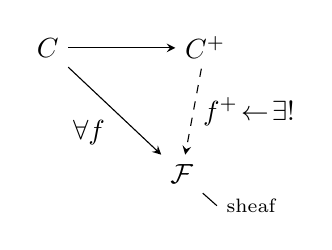
\begin{tikzpicture}[x=1cm,y=1cm,>=stealth]
  \node (c) at (0,1.6) {$C$};
  \node (plus) at (2.0,1.6) {$C^+$};
  \node (f) at (1.7,0) {$\mathcal F$};
  \draw[->] (c) -- (plus);
  \draw[->] (c) -- node[below left] {$\forall f$} (f);
  \draw[->,dashed] (plus) -- node[right] {$f^+\!\leftarrow\!\exists!$} (f);
  \draw (f.south east) -- ++(.18,-.16) node[right] {\scriptsize sheaf};
\end{tikzpicture}}\endgroup}
\end{GelfandAdjacentEvidence}
\begin{GelfandAdjacentEvidence}{GELFAND-P001386}{2}


\(\forall\) map \(f\colon C\longrightarrow\mathcal F\)
[below \(\mathcal F\): sheaf]
\(\exists!\ f^+\colon C^+\longrightarrow\mathcal F\), such that the diagram commutes

\uline{Exercise 1.}
[crossed out: “про…”?]
construct \(C^+\).

\Unclear{GELFAND-P001386}{cancelled-exercise}{“про…”?}
\end{GelfandAdjacentEvidence}
\begin{GelfandAdjacentEvidence}{GELFAND-P001386}{3}



There are maps
\[
\operatorname{Ker}\varphi\overset{\alpha}{\longrightarrow}\mathcal F
\overset{\varphi}{\longrightarrow}G
\overset{\beta}{\longrightarrow}\operatorname{Coker}\varphi
\]

\uline{Exercise 2.}\quad \(\operatorname{Ker}\beta=\operatorname{Coker}\alpha\)

An exact sequence of sheaves is defined in the natural way.

\uline{Exercise 3.}\quad
The sequence \(\mathcal F_1\longrightarrow\mathcal F_2\longrightarrow\mathcal F_3\)
is exact \(\Longleftrightarrow\ \forall x\in X\)
the sequence \(\mathcal F_{1x}\longrightarrow\mathcal F_{2x}\longrightarrow\mathcal F_{3x}\)
is exact.

(Consider the inclusion \(x\overset{i_x}{\longrightarrow}X\), then the stalk
\(\mathcal F_x\) at the point \(x\) has the form \(\mathcal F_x=i_x^*\mathcal F\))

\uline{Definition 2} (\uline{Flabby sheaf}.)

A sheaf \(\mathcal F\) is called flabby if any section over an open set \(V\) extends to a section over all of \(X\),
i.e. \(\forall\) open \(V\subset X\)
\[
\mathcal F(X)\longrightarrow\mathcal F(V)
\]
is an epimorphism.

\SourceFigure{GELFAND-P001386}{path-diagram}{%
\begingroup\color{black}\GelfandFitDiagram{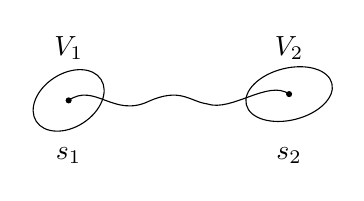
\begin{tikzpicture}[x=1cm,y=1cm]
  \draw[rotate around={33:(0,0)}] (0,0) ellipse (.49 and .34);
  \draw[rotate around={14:(2.8,.08)}] (2.8,.08) ellipse (.56 and .33);
  \draw (0,0) .. controls (.33,.23) and (.57,-.22) .. (1.01,-.015)
    .. controls (1.42,.17) and (1.53,-.01) .. (1.76,-.045)
    .. controls (2.07,-.15) and (2.54,.27) .. (2.8,.08);
  \fill (0,0) circle (1.1pt) (2.8,.08) circle (1.1pt);
  \node at (0,.66) {$V_1$}; \node at (2.8,.66) {$V_2$};
  \node at (0,-.70) {$s_1$}; \node at (2.8,-.70) {$s_2$};
\end{tikzpicture}}\endgroup\par The lower labels read \(s_1\), \(s_2\), possibly \(\xi_1\), \(\xi_2\).}
\end{GelfandAdjacentEvidence}


In locally constant sheaves, sections can be transported [inserted above the line: (along a path)] and therefore such sheaves are \uline{not flabby}.

\uline{Problem 4.}\quad \(\Gamma\) --- a
[inserted above the line: finite] ordered set; introduce the topology
\[
\overline{x}:=\{y:\ y\leq x\}\quad\text{--- closure of the point }x
\]
a) Sheaves on \(\Gamma\) \(=\) representations of \(\Gamma\)

b) Describe the flabby sheaves on \(\Gamma\)


\Needspace{7\baselineskip}
\begin{GelfandAdjacentEvidence}{GELFAND-P001387}{1}
\SourcePage{GELFAND-P001387}{2}

c) Connection with combinatorial sheaves

Suppose \(X\) has a stratification, consider the map
\SourceFigure{GELFAND-P001387}{stratum-map}{%
\begingroup\color{black}\GelfandFitDiagram{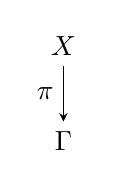
\begin{tikzpicture}[>=stealth]
  \node (space) at (0,1.2) {$X$};
  \node (strata) at (0,0) {$\Gamma$};
  \draw[->] (space) -- node[left] {$\pi$} (strata);
\end{tikzpicture}}\endgroup}
\end{GelfandAdjacentEvidence}
\begin{GelfandAdjacentEvidence}{GELFAND-P001387}{2}

(to the point \(x\) --- its stratum)

\(\Gamma\) --- ordered set of strata.

[below \(\Gamma\):] Give \(\Gamma\) the (Zariski) topology

\uline{Claim.}

\uwave{\(\forall\) combinatorial sheaf on \(X\) is the inverse image of}
[crossed out: “пучков” (of sheaves)?]
\uwave{a sheaf on \(\Gamma\)}
(and conversely)


\Unclear{GELFAND-P001387}{cancelled-pullback}{“пучков” (of sheaves)?}
\end{GelfandAdjacentEvidence}
\begin{GelfandAdjacentEvidence}{GELFAND-P001387}{3}

\[
\pi^*\colon\text{sheaves on }\Gamma\overset{\sim}{\longrightarrow}
\text{combinatorial sheaves on }X.
\]

\uline{Exercise 5.}\quad a) Suppose
\[
0\longrightarrow\mathcal F_1\longrightarrow\mathcal F_2\longrightarrow
\mathcal F_3\longrightarrow0
\]
is a short exact sequence of sheaves. Then the sequence of sections
\[
0\longrightarrow\mathcal F_1(X)\longrightarrow\mathcal F_2(X)
\longrightarrow\mathcal F_3(X)
\]
is exact.

b) If \(\mathcal F_1\) is flabby, the following sequence is exact
\[
0\longrightarrow\mathcal F_1(X)\longrightarrow\mathcal F_2(X)
\longrightarrow\mathcal F_3(X)\longrightarrow0
\]

\uline{Flabby resolution of a sheaf.}

\uline{Exercise 6}\quad Let \(\mathcal F\) be a sheaf. Then 1) It can be embedded in a flabby sheaf
\(\mathcal F\hookrightarrow G\).

2) Now construct from \(\mathcal F\) an exact sequence

\SourceFigure{GELFAND-P001387}{flabby-resolution-diagram}{%
\resizebox{\linewidth}{!}{%
\begingroup\color{black}\GelfandFitDiagram{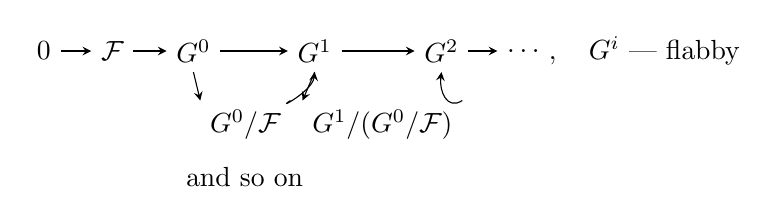
\begin{tikzpicture}[x=1cm,y=1cm,>=stealth]
  \node (zero) at (0,0) {$0$};
  \node (f) at (.87,0) {$\mathcal F$};
  \node (g0) at (1.9,0) {$G^0$};
  \node (g1) at (3.44,0) {$G^1$};
  \node (g2) at (5.05,0) {$G^2$};
  \node (tail) at (6.09,0) {$\ldots$};
  \node (q0) at (2.56,-.94) {$G^0/\mathcal F$};
  \node (q1) at (4.30,-.94) {$G^1/(G^0/\mathcal F)$};
  \node[right] at (6.29,0) {$,\quad G^i$ --- flabby};
  \draw[->] (zero) -- (f);
  \draw[->] (f) -- (g0);
  \draw[->] (g0) -- (g1);
  \draw[->] (g1) -- (g2);
  \draw[->] (g2) -- (tail);
  \draw[->] (g0.south) -- (q0.north west);
  \draw[->] (q0.north east) to[out=213,in=-97,looseness=1.35] (g1.south);
  \draw[->] (g1.south) -- (q1.north west);
  \draw[->] (q1.north east) to[out=213,in=-97,looseness=1.35] (g2.south);
  \node at (2.55,-1.60) {and so on};
\end{tikzpicture}}\endgroup}}
\end{GelfandAdjacentEvidence}


(flabby resolution)

3) \(\forall\) two flabby resolutions can be embedded in a common third one.

\uline{Definition 3.}
\[
H^i(X,\mathcal F)=H^i\bigl(0\longrightarrow G^0(X)\longrightarrow
G^1(X)\longrightarrow\ldots\bigr)
\]
(here \(0\longrightarrow\mathcal F\longrightarrow G^0\longrightarrow
G^1\longrightarrow\ldots\) --- flabby resolution \(\mathcal F\))

On the right is the cohomology of a complex of vector spaces.

\uline{Definition 4.}\quad [crossed out: Dual sheaf.]
\uwave{Cohomology with compact support.}

Suppose \(X\) is locally compact. Then we can consider sections with compact support:
\(\mathcal F_c(X)\) --- sections with compact support on \(X\).


\Needspace{7\baselineskip}
\begin{GelfandAdjacentEvidence}{GELFAND-P001388}{1}
\SourcePage{GELFAND-P001388}{unlabelled}

\[
H_c^i(X,\mathcal F)=H^i\bigl(0\longrightarrow G_c^0(X)\longrightarrow
G_c^1(X)\longrightarrow\ldots\bigr)
\]

\uline{Definition 5.}\quad Dual sheaf.

Presheaf: \(\mathcal F^*(V)=\mathcal F_c(V)^*\)
(analogue: “distribution” or possibly “distributions”\textsuperscript{?})
\Unclear{GELFAND-P001388}{dual-note}{“distribution” or possibly “distributions”}
\end{GelfandAdjacentEvidence}


(dual space in the sense of linear algebra)
\[
V_1\subset V_2\ \Rightarrow\ \mathcal F_c(V_1)\longrightarrow\mathcal F_c(V_2)
\quad\text{(embedding)}
\]
and this gives \(\mathcal F^*(V_2)\longrightarrow\mathcal F^*(V_1)\)

\uline{Exercise 7.}

a) \(\mathcal F^*\) is a sheaf if \(\mathcal F\) is flabby.

b) If \(\mathcal F^*\) is a sheaf, then \(\mathcal F^*\)
is flabby, i.e. \(\forall\underset{\text{open}}{V}\subset X\)
the map \(\mathcal F^*(X)\longrightarrow\mathcal F^*(V)\) is surjective


\Needspace{7\baselineskip}
\begin{GelfandAdjacentEvidence}{GELFAND-P001389}{1}
\SourcePage{GELFAND-P001389}{unlabelled}

\uline{12 October 1987.}\qquad \uline{Gelfand Seminar.}

Vakhtangov told the actors in Princess Turandot to come on stage in fashionable clothes and change at once (put on a turban, etc.). The themes of mathematics are eternal, only the language changes.

\uline{I. M. G.}\quad \uline{On a combinatorial conjecture of Dyson, connected with polynomial coefficients}

\uwave{A paper from the thick green collection on combinatorics}

Consider
\begin{equation*}
F(x,a)=\prod_{i\ne j}\left(1-\frac{x_j}{x_i}\right)^{a_j},
\qquad a_j\in\mathbb N.
\tag{1}
\end{equation*}
Find the constant term

Dyson's conjecture (1962), the answer
\begin{equation*}
\frac{(a_1+a_2\ldots+a_n)!}{a_1!a_2!\ldots a_n!}
\tag{2}
\end{equation*}

In 1962 two proofs were given in J. Math. Phys. (long ones)

In 1970 in J. Math. Phys., a proof by
\EvidenceBlock{GELFAND-P001389}{author-name}{Vuda}{Manuscript notation.}
\end{GelfandAdjacentEvidence}
\begin{GelfandAdjacentEvidence}{GELFAND-P001389}{2}

in two lines.

\uline{Proof}\quad Applying Lagrange's interpolation formula to the function \(f\equiv0\)
\EvidenceBlock{GELFAND-P001389}{interpolation-function}{The manuscript reads \(f\equiv0\).}{Manuscript notation.}
\end{GelfandAdjacentEvidence}

and then setting \(x=0\), we obtain
\begin{equation*}
\sum_j\prod_{i\ne j}\left(1-\frac{x_j}{x_i}\right)^{-1}=1
\tag{3}
\end{equation*}

Multiplying by \(F(x,a)\), we obtain


\Needspace{7\baselineskip}
\begin{GelfandAdjacentEvidence}{GELFAND-P001390}{1}
\SourcePage{GELFAND-P001390}{unlabelled}

\begin{equation*}
\sum_j F(x,a_1,\ldots,a_{j-1},a_j-1,a_{j+1},\ldots,a_n)=F(x,a)
\tag{4}
\end{equation*}

[crossed out: illegible opening mark\textsuperscript{?}]
\Unclear{GELFAND-P001390}{cancelled-let}{illegible opening mark}
\end{GelfandAdjacentEvidence}
\begin{GelfandAdjacentEvidence}{GELFAND-P001390}{2}

Let \(G(a)\) be the constant term. Then from (4)
\begin{equation*}
G(a)=\sum G(a_1,\ldots,a_{j-1},a_j-1,a_{j+1},\ldots,a_n),
\tag{5}
\end{equation*}
which gives a recurrence formula.

When \(a_j=0\) we obtain
\begin{equation*}
\begin{aligned}
G(a_1,\ldots,a_{j-1},0,a_{j+1},\ldots,a_n)
&=G(a_1,\ldots,a_{j-1},a_{j+1},\ldots,a_n)
\end{aligned}
\tag{6}
\end{equation*}
Moreover,
\begin{equation*}
G(0)=1
\tag{7}
\end{equation*}
The relations (5)--(7) are sufficient as recurrence relations. They determine everything and yield (2).

\uuline{A. Veselov}

\uline{On geodesics on an ellipsoid and motion on a sphere}

Following Jacobi and others, 1982. Knörrer's observation: equivalence of two problems.

[Two columns separated by a curved line. Left column.]

1) \((Aq,q)=1\)

geodesics on the ellipsoid

Weierstrass found them in \(\theta\)-functions (1861)

Equation of the geodesics in the natural parameter:
\begin{equation*}
\ddot q=\lambda Aq
\tag{1}
\end{equation*}
(acceleration \(\sim\) the normal)

[At right:] (\(\lambda\) is the Lagrange multiplier, found from the condition \((Aq,q)=1\))

[Right column.]

2) Another problem [crossed out:
\(C.\) the name after the initial is struck through, possibly “Neu…”\textsuperscript{?}]
\Unclear{GELFAND-P001390}{cancelled-neumann}{\(C.\) the name after the initial is struck through, possibly “Neu…”}
\end{GelfandAdjacentEvidence}
\begin{GelfandAdjacentEvidence}{GELFAND-P001390}{3}

C. Neumann (1859)

Motion with potential energy
\[
U(x)=\frac12(Ax,x)
\]
on the sphere \(\lvert x\rvert^2=1\)

Here the equation is
\begin{equation*}
x''=-Ax+ux
\tag{\(1'\)}
\end{equation*}
or in coordinates
\begin{equation*}
x_i''=-a_i x_i+ux_i
\tag{\(1''\)}
\end{equation*}
[a symbol is crossed out at right:
\(q\)? / \(u\)?\textsuperscript{?}]
\Unclear{GELFAND-P001390}{equation-end}{\(q\)? / \(u\)?}
\end{GelfandAdjacentEvidence}
\begin{GelfandAdjacentEvidence}{GELFAND-P001390}{4}


[Below the columns.]

Switch to another parameter
\begin{equation*}
q''=-Aq+vq'
\tag{2}
\end{equation*}
(the changes can be written out explicitly,
\(\underset{\substack{\parallel\\\mathrm{const}}}{\lambda}\rightsquigarrow
\underset{\substack{\parallel\\\mathrm{const}}}{v}\))
\Unclear{GELFAND-P001390}{constants-note}{The manuscript has “const” beneath \(\lambda\) and \(v\), with two short strokes above each inscription. The function of the strokes is unclear.}
\end{GelfandAdjacentEvidence}
\begin{GelfandAdjacentEvidence}{GELFAND-P001390}{5}


and then the substitution
\begin{equation*}
x=\frac{Aq}{\lvert Aq\rvert}\qquad\text{(Gauss substitution)}
\tag{3}
\end{equation*}
takes solutions of problem 1) to solutions of problem 2) (direct computation)
\EvidenceBlock{GELFAND-P001390}{bijection-note}{The manuscript reads “прямая выкладка” (direct computation).}{Manuscript notation.}
\end{GelfandAdjacentEvidence}


(H. Knörrer, 1982)

Equation

[At right:] Introduce the operator:
\begin{equation*}
L=-\frac{d^2}{dt^2}+u,\qquad Lx_i=a_i x_i
\tag{4}
\end{equation*}
(\(x_i\) --- eigenfunction!!)


\Needspace{7\baselineskip}
\SourcePage{GELFAND-P001391}{12}

At left:
\begin{equation*}
\widetilde L=-\frac{d^2}{dt^2}+v\frac{d}{dt}
\tag{5}
\end{equation*}
(conjugate to \(L\) by the Gauss substitution or the Miura substitution)

Knörrer arrived at it through the Moser--Trubowitz isomorphism

\uwave{Consider problem 2)}

There are two symplectic forms.

\uline{Problem} (I. M. G.) There is a symmetric matrix \(A\) and a matrix \(K\) of rank one.
How, from the eigenvalues of \(A+K\) can one recover \(K\)? (\(A\) is fixed)

--- this is exactly Jacobi's formula.

\uline{V.}\quad For \(n=2\) introduce new coordinates
\begin{gather*}
M=[\dot x,x],\qquad\text{(angular momentum --- cross product)}\\
p=x
\end{gather*}

\(1^{\circ}\). Lie--Berezin--Kirillov bracket
\begin{gather*}
\{M_i,M_j\}=\varepsilon_{ijk}M_k\\
\{M_i,p_j\}=\varepsilon_{ijk}p_k\\
\{p_i,p_j\}=0
\end{gather*}

Hamiltonian
\[
2H=M^2+(Ap,p)
\]
Then
\[
\begin{cases}
\dot M_i=\{M_i,H\}\\
\dot p_i=\{p_i,H\}
\end{cases}
\qquad\text{--- the Neumann equations}
\]

\uwave{Second bracket}
\begin{gather*}
\varepsilon_{ijk}a_kM_k=\{M_i,M_j\}\\
\varepsilon_{ijk}a_kp_k=\{M_i,p_j\}\\
\varepsilon_{ijk}M_k=\{p_i,p_j\}
\end{gather*}

Hamiltonian \(F=\frac12p^2\)

\uwave{I. M. G.}\quad This agrees with what Arnold discussed

(see the previous notebook)

The system is Hamiltonian in both.


\Needspace{7\baselineskip}
\begin{GelfandAdjacentEvidence}{GELFAND-P001392}{1}
\SourcePage{GELFAND-P001392}{unlabelled}

\uuline{A. Beilinson.}\quad \uwave{Constructible sheaves} (continued)

Representations of a partially ordered set \(\Longleftrightarrow\)
[crossed out: possibly “constructible”\textsuperscript{?}]
combinatorial sheaves

\Unclear{GELFAND-P001392}{cancelled-equivalence}{possibly “constructible”}
\end{GelfandAdjacentEvidence}
\begin{GelfandAdjacentEvidence}{GELFAND-P001392}{2}



\SourceFigure{GELFAND-P001392}{interval-strata}{%
\begingroup\color{black}\GelfandFitDiagram{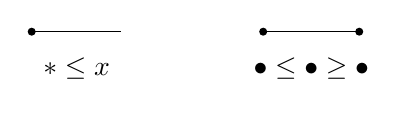
\begin{tikzpicture}[x=1cm,y=1cm]
  \draw (0,0) -- (1.14,0);
  \fill (0,0) circle (1.45pt);
  \draw (2.94,0) -- (4.16,0);
  \fill (2.94,0) circle (1.45pt) (4.16,0) circle (1.45pt);
  \node at (.57,-.47) {$\ast\leq x$};
  \node at (3.55,-.47) {$\bullet\leq\bullet\geq\bullet$};
\end{tikzpicture}}\endgroup}
\end{GelfandAdjacentEvidence}
\begin{GelfandAdjacentEvidence}{GELFAND-P001392}{3}


A combinatorial sheaf is a sheaf constant on each stratum.

\uwave{Homological algebra.}

\(\mathcal A\) --- abelian category (for example, of sheaves over a given space or of modules)

\(C(\mathcal A)\) --- category of complexes over \(\mathcal A\)

one needs to know the \uwave{derived category} (Verdier, 1961)

Objects of [crossed out:
possibly “из” (from) or a membership sign\textsuperscript{?}]
\(C(\mathcal A)\)


\Unclear{GELFAND-P001392}{objects-mark}{possibly “из” (from) or a membership sign}
\end{GelfandAdjacentEvidence}
\begin{GelfandAdjacentEvidence}{GELFAND-P001392}{4}

\begin{gather*}
\ldots\longrightarrow X^i\overset{d}{\longrightarrow}X^{i+1}
\overset{d}{\longrightarrow}X^{i+2}\longrightarrow\ldots\\
d^2=0
\end{gather*}
morphisms are morphisms of complexes (families of morphisms
\SourceFigure{GELFAND-P001392}{component-morphism}{%
\begingroup\color{black}\GelfandFitDiagram{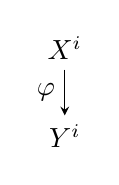
\begin{tikzpicture}[>=stealth]
  \node (x) at (0,1.12) {$X^i$};
  \node (y) at (0,0) {$Y^i$};
  \draw[->] (x) -- node[left] {$\varphi$} (y);
\end{tikzpicture}}\endgroup}
\end{GelfandAdjacentEvidence}
\begin{GelfandAdjacentEvidence}{GELFAND-P001392}{5}

, commuting with \(d\))

\(C(\mathcal A)\) --- also an abelian category

Bounded complexes (only finitely many \(\ne0\)) \(C^b(\mathcal A)\)

bounded on the left or the right \(C^{\pm}(\mathcal A)\)
\begin{gather*}
C^+(\mathcal A)\text{ --- bounded on the left}\\
C^-(\mathcal A)\text{ --- bounded on the right}
\end{gather*}

Homotopy category \(K(\mathcal A)\)

the objects of \(K(\mathcal A)\) are the same as in \(C(\mathcal A)\),
and the morphisms are equivalence classes of morphisms of \(C(\mathcal A)\) with respect to homotopy.
\[
\operatorname{Hom}_{K(\mathcal A)}(X^\bullet,Y^\bullet)
\]

A morphism \(X^\bullet\overset{\varphi}{\longrightarrow}Y^\bullet\)
is a [inserted above the line: such] family
\(\varphi^i\colon X^i\longrightarrow Y^i\), for which the diagram commutes:

\SourceFigure{GELFAND-P001392}{homotopy-diagrams}{%
\resizebox{\linewidth}{!}{%
\begingroup\color{black}\GelfandFitDiagram{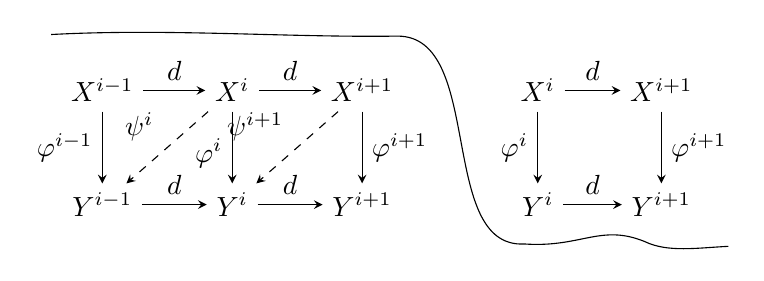
\begin{tikzpicture}[x=1cm,y=1cm,>=stealth]
  \node (xm) at (0,1.45) {$X^{i-1}$};
  \node (x) at (1.65,1.45) {$X^i$};
  \node (xp) at (3.3,1.45) {$X^{i+1}$};
  \node (ym) at (0,0) {$Y^{i-1}$};
  \node (y) at (1.65,0) {$Y^i$};
  \node (yp) at (3.3,0) {$Y^{i+1}$};
  \node (rx) at (5.53,1.45) {$X^i$};
  \node (rxp) at (7.10,1.45) {$X^{i+1}$};
  \node (ry) at (5.53,0) {$Y^i$};
  \node (ryp) at (7.10,0) {$Y^{i+1}$};
  \draw[->] (xm) -- node[above] {$d$} (x);
  \draw[->] (x) -- node[above] {$d$} (xp);
  \draw[->] (ym) -- node[above] {$d$} (y);
  \draw[->] (y) -- node[above] {$d$} (yp);
  \draw[->] (xm) -- node[left] {$\varphi^{i-1}$} (ym);
  \draw[->] (x) -- node[left,pos=.58] {$\varphi^i$} (y);
  \draw[->] (xp) -- node[right] {$\varphi^{i+1}$} (yp);
  \draw[->,dashed] (x) -- node[above left,pos=.55] {$\psi^i$} (ym);
  \draw[->,dashed] (xp) -- node[above left,pos=.55] {$\psi^{i+1}$} (y);
  \draw[->] (rx) -- node[above] {$d$} (rxp);
  \draw[->] (ry) -- node[above] {$d$} (ryp);
  \draw[->] (rx) -- node[left] {$\varphi^i$} (ry);
  \draw[->] (rxp) -- node[right] {$\varphi^{i+1}$} (ryp);
  \draw[thin] (-.65,2.16) .. controls (.84,2.24) and (2.35,2.12) .. (3.75,2.14)
    .. controls (4.86,2.14) and (4.25,-.56) .. (5.36,-.50)
    .. controls (6.08,-.55) and (6.33,-.24) .. (6.89,-.47)
    .. controls (7.18,-.61) and (7.55,-.55) .. (7.95,-.53);
\end{tikzpicture}}\endgroup}}
\end{GelfandAdjacentEvidence}


\(\varphi\) is called \uwave{null-homotopic}, if
\(\exists\) a family of maps \(X^i\overset{\psi^i}{\longrightarrow}Y^{i-1}\),
such that
\begin{equation*}
\varphi^i=d\psi^i+\psi^{i+1}d
\tag{1}
\end{equation*}


\Needspace{7\baselineskip}
\begin{GelfandAdjacentEvidence}{GELFAND-P001393}{1}
\SourcePage{GELFAND-P001393}{13}

\uline{Exercise 1.}\quad Check that for any system of maps \(\psi^i\) the family (1)
gives a morphism of complexes, i.e. \(d\varphi_i=\varphi_{i+1}d\).

\uline{Exercise 2.}\quad Morphisms homotopic to \(0\) form an ideal, i.e. if
\(\varphi\) is homotopic to \(0\) and \(\psi_1\) is any morphism,
\Unclear{GELFAND-P001393}{composition-symbol}{The first symbol is heavily retraced and provisionally reads \(\psi_1\),
and in the composition the symbol is \(\varphi_1\).}
\end{GelfandAdjacentEvidence}
\begin{GelfandAdjacentEvidence}{GELFAND-P001393}{2}

then \(\varphi\circ\varphi_1\) is homotopic to \(0\).

(and the same is true for the composition \(\varphi_2\circ\varphi\) with any morphism \(\varphi_2\))
\[
\begin{aligned}
\operatorname{Hom}_{K(\mathcal A)}(X^\bullet,Y^\bullet)
&=\operatorname{Hom}_{C(\mathcal A)}(X^\bullet,Y^\bullet)\\
&\qquad /\bigl(\text{morphisms homotopic to }0\bigr)
\end{aligned}
\]

There are obvious functors
\[
\mathcal A\longrightarrow C(\mathcal A)\longrightarrow K(\mathcal A)
\]

Cohomology functor
\[
H^i\colon C(\mathcal A)\longrightarrow\mathcal A\qquad
\left(H^i(X^\bullet)=
\frac{\ker(d\colon X^i\longrightarrow X^{i+1})}
{\operatorname{Im}(d\colon X^{i-1}\longrightarrow X^i)}\right)
\]

\uline{Exercise 3.}\quad Prove that \(\exists!\) a functor
\(H^i\colon K(\mathcal A)\longrightarrow\mathcal A\), such that
\SourceFigure{GELFAND-P001393}{cohomology-factorization}{%
\begingroup\color{black}\GelfandFitDiagram{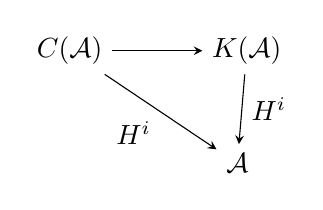
\begin{tikzpicture}[>=stealth]
  \node (c) at (0,1.43) {$C(\mathcal A)$};
  \node (k) at (2.25,1.43) {$K(\mathcal A)$};
  \node (a) at (2.13,0) {$\mathcal A$};
  \draw[->] (c) -- (k);
  \draw[->] (c) -- node[below left] {$H^i$} (a);
  \draw[->] (k) -- node[right] {$H^i$} (a);
\end{tikzpicture}}\endgroup}
\end{GelfandAdjacentEvidence}
\begin{GelfandAdjacentEvidence}{GELFAND-P001393}{3}


On morphisms \(H^i\) is also defined in the obvious way.

\uline{Definition.}
\[
\varphi\colon X^\bullet
\underset{\text{in the category }K(\mathcal A)}{\longrightarrow}Y^\bullet
\]
is called \uwave{a quasi-isomorphism} if it induces an isomorphism
\[
H^i(X^\bullet)\longrightarrow H^i(Y^\bullet).
\]

\uwave{Derived category}

\uwave{Exercise 4.}\quad Suppose there are three complexes
\SourceFigure{GELFAND-P001393}{fraction-span}{%
\begingroup\color{black}\GelfandFitDiagram{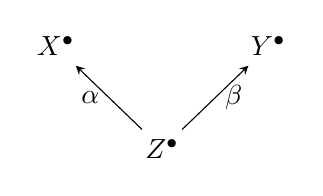
\begin{tikzpicture}[>=stealth]
  \node (x) at (0,1.3) {$X^\bullet$};
  \node (y) at (2.7,1.3) {$Y^\bullet$};
  \node (z) at (1.35,0) {$Z^\bullet$};
  \draw[->] (z) -- node[left] {$\alpha$} (x);
  \draw[->] (z) -- node[right] {$\beta$} (y);
\end{tikzpicture}}\endgroup}
\end{GelfandAdjacentEvidence}
\begin{GelfandAdjacentEvidence}{GELFAND-P001393}{4}

and morphisms, with \(\alpha\) --- a quasi-isomorphism.

Then there is a diagram (commutative)
\SourceFigure{GELFAND-P001393}{fraction-square}{%
\begingroup\color{black}\GelfandFitDiagram{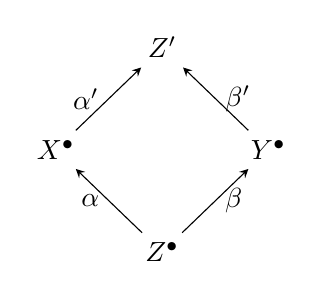
\begin{tikzpicture}[>=stealth]
  \node (x) at (0,1.3) {$X^\bullet$};
  \node (y) at (2.7,1.3) {$Y^\bullet$};
  \node (z) at (1.35,0) {$Z^\bullet$};
  \node (zp) at (1.35,2.6) {$Z'$};
  \draw[->] (z) -- node[left] {$\alpha$} (x);
  \draw[->] (z) -- node[right] {$\beta$} (y);
  \draw[->] (x) -- node[left] {$\alpha'$} (zp);
  \draw[->] (y) -- node[right] {$\beta'$} (zp);
\end{tikzpicture}}\endgroup}
\end{GelfandAdjacentEvidence}
\begin{GelfandAdjacentEvidence}{GELFAND-P001393}{5}

[crossed out to the left of the diagram:
“in which”?\textsuperscript{?}.]
\Unclear{GELFAND-P001393}{cancelled-left}{“in which”?}
\end{GelfandAdjacentEvidence}
\begin{GelfandAdjacentEvidence}{GELFAND-P001393}{6}


in which \(\beta'\) --- a quasi-isomorphism.

The same is true if we start with the diagram
\SourceFigure{GELFAND-P001393}{fraction-cospan}{%
\begingroup\color{black}\GelfandFitDiagram{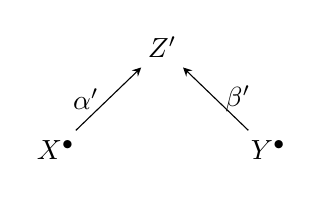
\begin{tikzpicture}[>=stealth]
  \node (x) at (0,0) {$X^\bullet$};
  \node (y) at (2.7,0) {$Y^\bullet$};
  \node (zp) at (1.35,1.3) {$Z'$};
  \draw[->] (x) -- node[left] {$\alpha'$} (zp);
  \draw[->] (y) -- node[right] {$\beta'$} (zp);
\end{tikzpicture}}\endgroup}
\end{GelfandAdjacentEvidence}

with quasi-isomorphism \(\alpha'\).


\Needspace{7\baselineskip}
\begin{GelfandAdjacentEvidence}{GELFAND-P001394}{1}
\SourcePage{GELFAND-P001394}{unlabelled}

\uwave{Derived category} \(D(\mathcal A)\)

Objects \(=\) objects of \(K(\mathcal A)\) (i.e. complexes)

Morphisms [inserted above the line: \(X^\bullet\longrightarrow Y^\bullet\)] ---
equivalence classes of diagrams
\SourceFigure{GELFAND-P001394}{derived-roof}{%
\begingroup\color{black}\GelfandFitDiagram{\begin{tikzpicture}[>=stealth]
  \node (x) at (0,1.3) {$X^\bullet$};
  \node (y) at (2.7,1.3) {$Y^\bullet$};
  \node (z) at (1.35,0) {$Z^\bullet$};
  \node at (4.12,.66) {$\beta\alpha^{-1}$};
  \draw[->] (z) -- node[left] {$\alpha$} (x);
  \draw[->] (z) -- node[right] {$\beta$} (y);
\end{tikzpicture}}\endgroup}
\end{GelfandAdjacentEvidence}
\begin{GelfandAdjacentEvidence}{GELFAND-P001394}{2}


(\(\alpha\) --- a quasi-isomorphism)

under the equivalence relation \uwave{generated} by the elem. relation
\EvidenceBlock{GELFAND-P001394}{elementary-abbrev}{The manuscript abbreviation is “элем.” (elem.).}{Manuscript notation.}
\end{GelfandAdjacentEvidence}
\begin{GelfandAdjacentEvidence}{GELFAND-P001394}{3}


[crossed out: “There is”? / “If”?\textsuperscript{?}.]
\Unclear{GELFAND-P001394}{cancelled-there}{“There is”? / “If”?}
\end{GelfandAdjacentEvidence}
\begin{GelfandAdjacentEvidence}{GELFAND-P001394}{4}


(There is a functor \(K(\mathcal A)\longrightarrow D(\mathcal A)\))

\SourceFigure{GELFAND-P001394}{roof-refinement}{%
\begingroup\color{black}\GelfandFitDiagram{\begin{tikzpicture}[>=stealth]
  \node (x) at (0,2.6) {$X^\bullet$};
  \node (y) at (2.7,2.6) {$Y^\bullet$};
  \node (z) at (1.35,1.28) {$Z^\bullet$};
  \node (t) at (1.35,0) {$T$};
  \draw[->] (z) -- node[left] {$\alpha$} (x);
  \draw[->] (z) -- node[right] {$\beta$} (y);
  \draw[->] (t) -- node[right] {$\gamma$} (z);
\end{tikzpicture}}\endgroup}
\end{GelfandAdjacentEvidence}
\begin{GelfandAdjacentEvidence}{GELFAND-P001394}{5}


\(\beta\alpha^{-1}\sim\beta\gamma(\alpha\gamma)^{-1}\),
where \(\gamma\) --- a quasi-isomorphism.
\Unclear{GELFAND-P001394}{fraction-relation}{The relation sign resembles \(\sim\). Retracing obscures individual strokes in the sign and the following \(\beta\).}
\end{GelfandAdjacentEvidence}
\begin{GelfandAdjacentEvidence}{GELFAND-P001394}{6}


\SourceFigure{GELFAND-P001394}{equivalent-roofs}{%
\resizebox{\linewidth}{!}{%
\begingroup\color{black}\GelfandFitDiagram{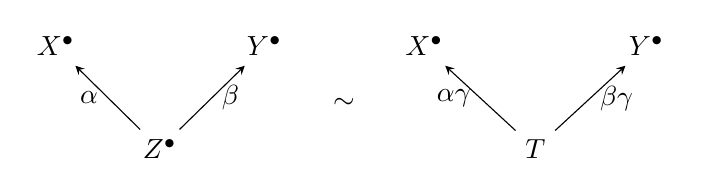
\begin{tikzpicture}[>=stealth]
  \node (x) at (0,1.30) {$X^\bullet$};
  \node (y) at (2.65,1.30) {$Y^\bullet$};
  \node (z) at (1.32,0) {$Z^\bullet$};
  \node at (3.66,.58) {$\sim$};
  \node (rx) at (4.68,1.30) {$X^\bullet$};
  \node (ry) at (7.50,1.30) {$Y^\bullet$};
  \node (t) at (6.09,0) {$T$};
  \draw[->] (z) -- node[left] {$\alpha$} (x);
  \draw[->] (z) -- node[right] {$\beta$} (y);
  \draw[->] (t) -- node[left] {$\alpha\gamma$} (rx);
  \draw[->] (t) -- node[right] {$\beta\gamma$} (ry);
\end{tikzpicture}}\endgroup}}
\end{GelfandAdjacentEvidence}
\begin{GelfandAdjacentEvidence}{GELFAND-P001394}{7}


We can now compose the morphisms.

\SourceFigure{GELFAND-P001394}{roof-composition}{%
\resizebox{\linewidth}{!}{%
\begingroup\color{black}\GelfandFitDiagram{\begin{tikzpicture}[>=stealth]
  \node (x) at (0,2.45) {$X^\bullet$};
  \node (y) at (2.6,2.45) {$Y^\bullet$};
  \node (w) at (5.2,2.45) {$W$};
  \node (z) at (1.30,1.2) {$Z^\bullet$};
  \node (t) at (3.90,1.2) {$T$};
  \node (s) at (2.6,-.12) {$S$};
  \draw[->] (z) -- (x);
  \draw[->] (z) -- (y);
  \draw[->] (t) -- (y);
  \draw[->] (t) -- (w);
  \draw[->] (s) -- (z);
  \draw[->] (s) -- (t);
  \draw[->] (4.84,.34) -- (4.13,.34);
  \node[right,align=left] at (4.93,.34) {complete by \uwave{the lemma}};
\end{tikzpicture}}\endgroup}}
\end{GelfandAdjacentEvidence}


the composition is the outside of the diagram.


\Needspace{7\baselineskip}
\begin{GelfandAdjacentEvidence}{GELFAND-P001395}{1}
\SourcePage{GELFAND-P001395}{unlabelled}

\uline{19.10.87.}\quad \uline{Gelfand Seminar.}

\uwave{I. M. Gelfand}\quad \uuline{Calculation of sums of \(k\)th powers and other sums}

\Unclear{GELFAND-P001395}{speaker-parenthesis}{(following a recent idea?)}
\end{GelfandAdjacentEvidence}
\begin{GelfandAdjacentEvidence}{GELFAND-P001395}{2}


\[
F'(x)=f(x)\qquad f(x)=x^k,\qquad F(x)=\frac{x^{k+1}}{k+1}
\]
\begin{align*}
F(2)-F(1)&=\frac{f(1)}{1!}+\frac{f'(1)}{2!}+\frac{f''(1)}{3!}+\ldots\\
F(3)-F(2)&=\frac{f(2)}{1!}+\frac{f'(2)}{2!}+\frac{f''(2)}{3!}+\ldots\\[8pt]
F(n+1)-F(n)&=f(n)+\frac{f'(n)}{2!}+\frac{f''(n)}{3!}+\ldots
\end{align*}
\rule{9cm}{.3pt}
\[
F(n+1)-F(1)=S_0+\frac{S_1}{2!}+\frac{S_2}{3!}+\ldots
\]
similarly,
\begin{align*}
f(n+1)-f(1)&=S_1+\frac{S_2}{2!}+\ldots\\
f'(n+1)-f'(1)&=S_2+\frac{S_3}{2!}+\ldots\\
\ldots\qquad&\ldots\\
f^{(p)}(n+1)-f^{(p)}(1)&=\ldots\quad S_p+\ldots
\end{align*}
\EvidenceBlock{GELFAND-P001395}{system-last-index}{The last line has \(S_p\).}{Manuscript notation.}
\end{GelfandAdjacentEvidence}
\begin{GelfandAdjacentEvidence}{GELFAND-P001395}{3}


[To the right of the system] Here
\begin{align*}
S_0&=f(1)+f(2)+\ldots+f(n)\\
S_1&=f'(1)+f'(2)+\ldots+f'(n)\\
&\ldots\\
S_k&=f^{(k)}(1)+f^{(k)}(2)+\ldots+f^{(k)}(n)
\end{align*}

Hence
[crossed out to the left of the determinant:
“det”?\textsuperscript{?}]
\Unclear{GELFAND-P001395}{determinant-cancellation}{“det”?}
\end{GelfandAdjacentEvidence}
\begin{GelfandAdjacentEvidence}{GELFAND-P001395}{4}

\SourceFigure{GELFAND-P001395}{determinant-layout}{%
\(\displaystyle S_0=\frac{
\begin{vmatrix}
F(n+1)-F(1)&\frac{1}{2!}&\frac{1}{3!}&\ldots\\
f(n+1)-f(1)&1&\frac{1}{2!}&\\
f'(n+1)-f'(1)&0&1&\\
\ldots&0&0&
\end{vmatrix}}{1}\)}
\end{GelfandAdjacentEvidence}
\begin{GelfandAdjacentEvidence}{GELFAND-P001395}{5}


Expand along the first column
\[
S_0=A_0\bigl(F(n+1)-F(1)\bigr)
+A_1\bigl(f(n+1)-f(1)\bigr)+\ldots
\]
coefficients are universal, it works for \(\forall\) functions!!

Substitute \(f(x)=e^{tx}\)

banded determinants appear!

[crossed out:
possibly \(S_0=A_0\)\textsuperscript{?}]
\Unclear{GELFAND-P001395}{exponential-cancellation}{possibly \(S_0=A_0\)}
\end{GelfandAdjacentEvidence}
\begin{GelfandAdjacentEvidence}{GELFAND-P001395}{6}

\[
\frac{\dfrac{1}{n+1}e^{t(n+1)}-e}{e^t-1}
\]
\EvidenceBlock{GELFAND-P001395}{exponential-fraction}{Numerator
\(\frac{1}{n+1}e^{t(n+1)}-e\).}{Manuscript notation.}
\end{GelfandAdjacentEvidence}
\begin{GelfandAdjacentEvidence}{GELFAND-P001395}{7}

expand [crossed out:
“series”?\textsuperscript{?}]
\Unclear{GELFAND-P001395}{series-cancellation}{“series”?}
\end{GelfandAdjacentEvidence}
\begin{GelfandAdjacentEvidence}{GELFAND-P001395}{8}

in \(t\)\quad \(\Longrightarrow\) \uline{Bernoulli numbers}

\uline{Problem.} The symmetric group \(S_n\) is defined
\EvidenceBlock{GELFAND-P001395}{symmetric-group-predicate}{“Is defined” (определяется).}{Manuscript notation.}
\end{GelfandAdjacentEvidence}
\begin{GelfandAdjacentEvidence}{GELFAND-P001395}{9}

[inserted above the line: (obr[…]\textsuperscript{?} \(s_1,\ldots,s_{n-1}\))]
\Unclear{GELFAND-P001395}{group-generator-abbreviation}{The abbreviation begins “obr”. Its ending is unclear.}
\end{GelfandAdjacentEvidence}

by the relations
\[
s_i^2=1,\qquad s_i s_j=s_j s_i\quad\text{when }\lvert i-j\rvert\ge2,
\qquad (s_i s_{i+1})^3=1
\]
Consider the parabolic subgroup
\[
G=\Sigma_n,\qquad H=\Sigma_k\times\Sigma_{n-k},\qquad G\supset H
\]
\[
\mathcal A=\mathbb C[G]=
\left\{\sum_{g\in G}a_g g,\quad a_g\in\mathbb C\right\}
\]


\Needspace{7\baselineskip}
\begin{GelfandAdjacentEvidence}{GELFAND-P001396}{1}
\SourcePage{GELFAND-P001396}{23}

\[
\mathcal A\supset\underset{\substack{\vert\\\text{subalgebra}}}{\mathcal A'}
=\{x\in A,\ xh=hx=x\text{ for any }h\in H\}
\]

[crossed out: illegible mark\textsuperscript{?}]
\Unclear{GELFAND-P001396}{heading-cancellation}{illegible mark}
\end{GelfandAdjacentEvidence}
\begin{GelfandAdjacentEvidence}{GELFAND-P001396}{2}

\uuline{Beilinson, A.}\quad (continued)

\uline{Derived categories.}

\SourceFigure{GELFAND-P001396}{category-chain}{%
\resizebox{\linewidth}{!}{%
\begingroup\color{black}\GelfandFitDiagram{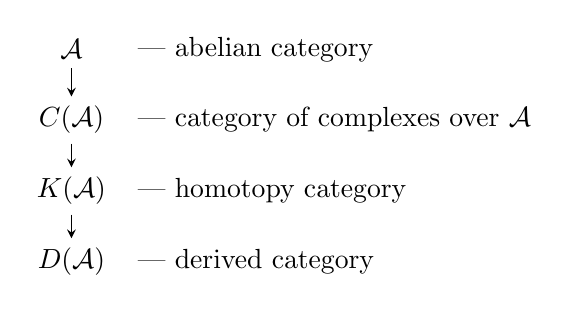
\begin{tikzpicture}[>=stealth]
  \node (a) at (0,2.7) {$\mathcal A$};
  \node (c) at (0,1.8) {$C(\mathcal A)$};
  \node (k) at (0,.9) {$K(\mathcal A)$};
  \node (d) at (0,0) {$D(\mathcal A)$};
  \node[right] at (.72,2.7) {--- abelian category};
  \node[right] at (.72,1.8) {--- category of complexes over \(\mathcal A\)};
  \node[right] at (.72,.9) {--- homotopy category};
  \node[right] at (.72,0) {--- derived category};
  \draw[->] (a) -- (c);
  \draw[->] (c) -- (k);
  \draw[->] (k) -- (d);
\end{tikzpicture}}\endgroup}}
\end{GelfandAdjacentEvidence}
\begin{GelfandAdjacentEvidence}{GELFAND-P001396}{3}


the objects of \(D(\mathcal A)\) are complexes, and the morphisms are equivalence classes of diagrams

\SourceFigure{GELFAND-P001396}{roof-cancellation}{%
\begingroup\color{black}\GelfandFitDiagram{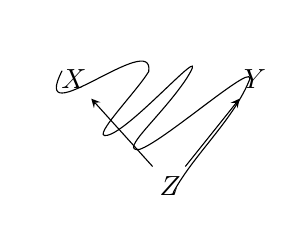
\begin{tikzpicture}[>=stealth]
  \node (x) at (0,1.35) {$X$};
  \node (y) at (2.30,1.35) {$Y$};
  \node (z) at (1.22,0) {$Z$};
  \draw[->] (z) -- (x);
  \draw[->] (z) -- (y);
  \draw (-.15,1.46) .. controls (-.58,.61) and (1.03,2.00) .. (.95,1.45)
    .. controls (.79,1.18) and (.11,.50) .. (.48,.66)
    .. controls (.84,.83) and (1.78,1.92) .. (1.43,1.36)
    .. controls (1.11,.88) and (.56,.43) .. (.83,.46)
    .. controls (1.15,.56) and (2.38,1.66) .. (2.22,1.32)
    .. controls (2.01,.82) and (1.51,.38) .. (1.26,-.09);
\end{tikzpicture}}\endgroup
\par{\small The diagram is crossed out. The right arrow is partly obscured.}}
\end{GelfandAdjacentEvidence}
\begin{GelfandAdjacentEvidence}{GELFAND-P001396}{4}


\SourceFigure{GELFAND-P001396}{shorter-roof-square}{%
\begingroup\color{black}\GelfandFitDiagram{\begin{tikzpicture}[>=stealth]
  \node (x) at (0,1.04) {$X$};
  \node (y) at (2.66,1.53) {$Y$};
  \node (z) at (.68,0) {$Z$};
  \node (zp) at (1.88,2.57) {$Z'$};
  \draw[->] (x) -- (zp);
  \draw[->] (z) -- (y);
  \draw[->,shorten <=4pt,shorten >=3pt] (y) -- (zp);
  \draw[->,shorten <=4pt,shorten >=3pt] (z) -- (x);
\end{tikzpicture}}\endgroup\par (quasi-isomorphisms are shorter).}
\end{GelfandAdjacentEvidence}
\begin{GelfandAdjacentEvidence}{GELFAND-P001396}{5}


\uline{Example 1.}\quad Let \(X\) be a complex with
[crossed out: possibly “со” (with)\textsuperscript{?}]
\(H^i(X)=0\) for \(i\ne0\).
Then \(X\) is canonically quasi-isomorphic to \(H^0(X)\):


\Unclear{GELFAND-P001396}{example-cancellation}{possibly “со” (with)}
\end{GelfandAdjacentEvidence}
\begin{GelfandAdjacentEvidence}{GELFAND-P001396}{6}

\[
X\cong H^0(X)\text{ in }D(\mathcal A)
\]
(In the homotopy category this is not so!)

For a complex \(X\) introduce the subcomplex \(\tau_{\leq0}(X)\in X\):
\begin{equation*}
\tau_{\leq0}(X)^i=
\begin{cases}
X^i,&i<0\\
\ker(d\colon X^0\to X^1),&i=0\\
0,&i>0
\end{cases}
\tag{1}
\end{equation*}

It is easy to see that
\begin{equation*}
H^j(\tau_{\leq0}(X))=
\begin{cases}
H^j(X),&j\leq0\\
0,&j>0
\end{cases}
\tag{2}
\end{equation*}
The diagram
\SourceFigure{GELFAND-P001396}{truncation-diagram}{%
\resizebox{\linewidth}{!}{%
\begingroup\color{black}\GelfandFitDiagram{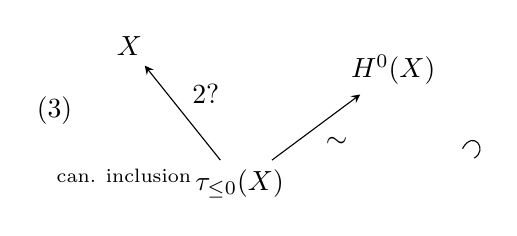
\begin{tikzpicture}[>=stealth]
  \node (x) at (0,1.75) {$X$};
  \node (h) at (3.35,1.45) {$H^0(X)$};
  \node (t) at (1.4,0) {$\tau_{\leq0}(X)$};
  \node at (-.95,.93) {(3)};
  \draw[->] (t) -- node[above right] {$2$?} (x);
  \draw[->] (t) -- node[below right] {$\sim$} (h);
  \node[align=left] at (-.07,.11) {\scriptsize can. inclusion};
  \draw[thin] (4.23,.45) .. controls (4.37,.70) and (4.56,.44) .. (4.38,.33);
\end{tikzpicture}}\endgroup}\par{\small The mark by the left arrow resembles a 2 or a rotated tilde.}}
\end{GelfandAdjacentEvidence}
\begin{GelfandAdjacentEvidence}{GELFAND-P001396}{7}

gives the required isomorphism in \(D(\mathcal A)\).

[crossed out:
This same complex can be projected onto…?\textsuperscript{?}]
\Unclear{GELFAND-P001396}{cancelled-bottom-sentence}{This same complex can be projected onto…?}
\end{GelfandAdjacentEvidence}
\begin{GelfandAdjacentEvidence}{GELFAND-P001396}{8}


\uline{Remark.} a complex \(X\) with several nonzero  cohomology groups \(H^i\) is
\uline{not} quasi-isomorphic (in general) to the sum, and if there
[inserted above the line: (quasi)] is one, the way is non-unique\textsuperscript{?}.
\Unclear{GELFAND-P001396}{ending-reading}{The ending reads “in a non-unique way”. The final letters of the first Russian word are unclear.}
\end{GelfandAdjacentEvidence}



\Needspace{7\baselineskip}
\begin{GelfandAdjacentEvidence}{GELFAND-P001397}{1}
\SourcePage{GELFAND-P001397}{unlabelled}

\uline{Structure of a triangulated category}

\(K(A)\) and \(D(A)\) are not abelian categories.

\uline{Exercise 1.}\quad Check that
\[
K(A)\text{ --- abelian}\quad\Longleftrightarrow\quad
\mathcal A\text{ is semisimple}
\]
(\(\mathcal A\) --- semisimple \(\Longleftrightarrow\
[(\forall\text{ object})=(\text{direct sum of irreducibles})]\)).

\uline{Cone of a morphism.}

Let \(f\colon X\longrightarrow Y\) be a morphism of complexes

\SourceFigure{GELFAND-P001397}{bicomplex-diagram}{%
\begingroup\color{black}\GelfandFitDiagram{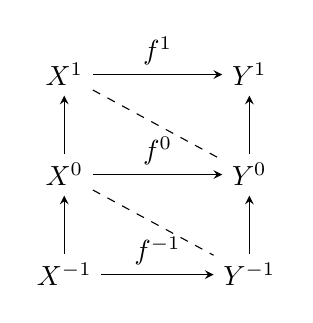
\begin{tikzpicture}[>=stealth]
  \node (x1) at (0,2.54) {$X^1$}; \node (y1) at (2.35,2.54) {$Y^1$};
  \node (x0) at (0,1.27) {$X^0$}; \node (y0) at (2.35,1.27) {$Y^0$};
  \node (xm) at (0,0) {$X^{-1}$}; \node (ym) at (2.35,0) {$Y^{-1}$};
  \draw[->] (x1) -- node[above] {$f^1$} (y1);
  \draw[->] (x0) -- node[above] {$f^0$} (y0);
  \draw[->] (xm) -- node[above] {$f^{-1}$} (ym);
  \draw[->] (xm) -- (x0); \draw[->] (x0) -- (x1);
  \draw[->] (ym) -- (y0); \draw[->] (y0) -- (y1);
  \draw[dashed] (x1) -- (y0); \draw[dashed] (x0) -- (ym);
\end{tikzpicture}}\endgroup}
\end{GelfandAdjacentEvidence}
\begin{GelfandAdjacentEvidence}{GELFAND-P001397}{2}

[At right] consider all this as a bicomplex, i.e. write the complex
\[
C(f)^i=Y^i\oplus X^{i+1}
\]
\EvidenceBlock{GELFAND-P001397}{cone-coordinate-order}{The cone formula has \(Y^i\oplus X^{i+1}\).}{Manuscript notation.}
\end{GelfandAdjacentEvidence}
\begin{GelfandAdjacentEvidence}{GELFAND-P001397}{3}

\[
d(x,y)=(-d(x),d(y)+f(x))
\]

There is a sequence
\begin{equation*}
C(f[-1])\longrightarrow X\overset{f}{\longrightarrow}Y
\underset{\substack{g\\\text{incl.}}}{\longrightarrow}C(f)
\longrightarrow X[1]\longrightarrow
\tag{4}
\end{equation*}
[Crossed out above the arrow \(Y\to C(f)\):
illegible entry\textsuperscript{?}.]
\Unclear{GELFAND-P001397}{sequence-arrow-cancellation}{illegible entry}
\end{GelfandAdjacentEvidence}
\begin{GelfandAdjacentEvidence}{GELFAND-P001397}{4}

[Crossed out before \(C(f)\):
\(X\)? / \(Y\)?\textsuperscript{?}.]
\Unclear{GELFAND-P001397}{sequence-object-cancellation}{\(X\)? / \(Y\)?}
\end{GelfandAdjacentEvidence}
\begin{GelfandAdjacentEvidence}{GELFAND-P001397}{5}

[Below \(X[1]\): the grading is shifted and the sign is changed on \(d\).]
\[
\longrightarrow Y(1)\longrightarrow C(f[1])\longrightarrow X[2]\longrightarrow
\]
\Unclear{GELFAND-P001397}{sequence-shifted-cone}{The closing parenthesis follows the shift: \(C(f[1])\). The crossed-out writing between \(f\) and \([1]\) is illegible.}
\end{GelfandAdjacentEvidence}
\begin{GelfandAdjacentEvidence}{GELFAND-P001397}{6}

[Between \(X\) and \([2]\) crossed out:
a mark resembling a parenthesis\textsuperscript{?}]
\Unclear{GELFAND-P001397}{sequence-shift-cancellation}{a mark resembling a parenthesis}
\end{GelfandAdjacentEvidence}
\begin{GelfandAdjacentEvidence}{GELFAND-P001397}{7}


it goes into itself under a shift of three steps.
In the homotopy category it goes into itself under a shift of one step.

\begin{equation*}
Y\overset{g}{\longrightarrow}C(f)\longrightarrow C(g)
\tag{5}
\end{equation*}

(6) \uline{Assertion.}\quad In \(K(A)\) the complex \(C(g)=X[1]\).

There is a map:
\SourceFigure{GELFAND-P001397}{cone-projection-diagram}{%
\begingroup\color{black}\GelfandFitDiagram{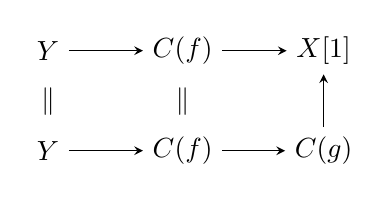
\begin{tikzpicture}[>=stealth]
  \node (y) at (0,1.27) {$Y$}; \node (ry) at (0,0) {$Y$};
  \node (f) at (1.71,1.27) {$C(f)$}; \node (rf) at (1.71,0) {$C(f)$};
  \node (x) at (3.50,1.27) {$X[1]$}; \node (g) at (3.50,0) {$C(g)$};
  \draw[->] (y) -- (f); \draw[->] (f) -- (x);
  \draw[->] (ry) -- (rf); \draw[->] (rf) -- (g);
  \node at (0,.63) {$\parallel$}; \node at (1.71,.63) {$\parallel$};
  \draw[->] (g) -- (x);
\end{tikzpicture}}\endgroup}
\end{GelfandAdjacentEvidence}


Namely,
\[
C(g)^i=C(f)^i\oplus Y^{i+1}=X^{i+1}\oplus Y^i\oplus Y^{i+1}
\]
projects to \(X^{i+1}\).


\Needspace{7\baselineskip}
\begin{GelfandAdjacentEvidence}{GELFAND-P001398}{1}
\SourcePage{GELFAND-P001398}{24}

\uline{Exercise 2.} Check that this is a morphism of complexes and an isomorphism in the homotopy category.

\uline{Exercise 3.} Find in \(K(A)\) the cones
\(C(\underset{\substack{\vert\\\text{identity map}}}{id})\)
and
\(C(\underset{\substack{\vert\\\text{zero map}}}{0})\).

\uline{Definition 1.} A triangle in \(K(A)\) or \(D(A)\) is the diagram

\SourceFigure{GELFAND-P001398}{triangle-sequence}{%
\begingroup\color{black}\GelfandFitDiagram{\(\begin{aligned}
\cdots\longrightarrow Z[-1]\xrightarrow{\gamma[-1]} X
  \xrightarrow{\alpha}Y\xrightarrow{\beta}Z\\
{}\xrightarrow{\gamma}X[1]\xrightarrow{\alpha[1]}Y[1]
  \xrightarrow{\beta[1]}Z[1]\xrightarrow{\gamma[1]}\cdots
\end{aligned}\)}\endgroup}
\end{GelfandAdjacentEvidence}
\begin{GelfandAdjacentEvidence}{GELFAND-P001398}{2}


\SourceFigure{GELFAND-P001398}{cancelled-sketch}{%
\begingroup\color{black}\GelfandFitDiagram{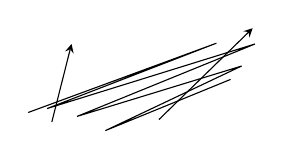
\begin{tikzpicture}[>=stealth,x=1cm,y=1cm]
  \draw[->] (.33,.03) -- (.58,1.02);
  \draw[->] (1.69,.06) -- (2.88,1.22);
  \draw[thin] (.03,.15) -- (2.42,1.03) -- (.27,.20) -- (2.91,1.02)
    -- (.65,.10) -- (2.74,.74) -- (1.01,-.08) -- (2.60,.57);
\end{tikzpicture}}\endgroup
\par{\small Crossed-out sketch. Two arrows are visible; any labels are illegible.}}
\end{GelfandAdjacentEvidence}
\begin{GelfandAdjacentEvidence}{GELFAND-P001398}{3}


\uuline{Def. 2.} An exact triangle in \(K(A)\) or \(D(A)\) is a triangle isomorphic to the triangle

\SourceFigure{GELFAND-P001398}{exact-triangle}{%
\begingroup\color{black}\GelfandFitDiagram{\(\longrightarrow X\xrightarrow{f}Y\xrightarrow{g}C(f)
  \longrightarrow X[1]\longrightarrow Y[1]\longrightarrow\cdots\)}\endgroup}
\end{GelfandAdjacentEvidence}



\Needspace{7\baselineskip}
\begin{GelfandAdjacentEvidence}{GELFAND-P001399}{1}
\SourcePage{GELFAND-P001399}{unlabelled}

\uline{9/XI-87 }\qquad \uuline{Gelfand seminar}

[Crossed out: Lascoux.]\qquad \uline{Lascoux}

\uline{I. M. G. after Lascoux}
(beautiful / regular\textsuperscript{?} series)

\Unclear{GELFAND-P001399}{heading-parenthesis}{beautiful / regular}
\end{GelfandAdjacentEvidence}
\begin{GelfandAdjacentEvidence}{GELFAND-P001399}{2}



Schubert polynomials.

Consider the polynomial
\begin{equation*}
P=\alpha u+\beta u+\gamma w+\cdots \tag{1}
\end{equation*}
\EvidenceBlock{GELFAND-P001399}{equation-1-second-variable}{The second monomial in (1) is \(\beta u\).}{Manuscript notation.}
\end{GelfandAdjacentEvidence}
\begin{GelfandAdjacentEvidence}{GELFAND-P001399}{3}


\(u,v,w\) [Crossed out: possibly \(\alpha,\beta,\gamma\)\textsuperscript{?}] are monomials.

\Unclear{GELFAND-P001399}{cancelled-coefficients}{possibly \(\alpha,\beta,\gamma\)}
\end{GelfandAdjacentEvidence}
\begin{GelfandAdjacentEvidence}{GELFAND-P001399}{4}



In our case we will have \(u,v,w,\)
[Crossed out: illegible mark]
\(\ldots=x_1,x_2,\ldots,x_n\).

\Unclear{GELFAND-P001399}{cancelled-after-w}{illegible mark}
\end{GelfandAdjacentEvidence}
\begin{GelfandAdjacentEvidence}{GELFAND-P001399}{5}



\(\alpha,\beta,\gamma,\ldots\) are numbers.

The polynomials [Crossed out: f-ia / f-i\textsuperscript{?}]
\(S^m(P)\) [Crossed out: possibly Schur\textsuperscript{?}]
are defined by the formula


\Unclear{GELFAND-P001399}{cancelled-before-sm}{“f-ia” / “f-i”?}
\end{GelfandAdjacentEvidence}
\begin{GelfandAdjacentEvidence}{GELFAND-P001399}{6}

\Unclear{GELFAND-P001399}{cancelled-after-sm}{possibly Schur}
\end{GelfandAdjacentEvidence}
\begin{GelfandAdjacentEvidence}{GELFAND-P001399}{7}

\begin{equation*}
\sum_{m\ge 0}^{\infty}z^m S^m(P)
=\frac{1}{(1-zu)^\alpha(1-zv)^\beta\ldots} \tag{2}
\end{equation*}
\EvidenceBlock{GELFAND-P001399}{equation-2-lower-bound}{The lower limit in (2) is \(m\ge 0\).}{Manuscript notation.}
\end{GelfandAdjacentEvidence}
\begin{GelfandAdjacentEvidence}{GELFAND-P001399}{8}


\[
\alpha=\beta=\gamma=\cdots=1\quad\Rightarrow
\]
\begin{equation*}
S^m(x_1+x_2+\cdots+x_n)
=\sum_{i_1\le i_2\le\cdots\le i_m}x_{i_1}x_{i_2}\cdots x_{i_m} \tag{3}
\end{equation*}

For example,
\[
S^2(x_1+x_2)=x_1^2+x_1x_2+x_2^2.
\]

Consider a Hankel matrix (of infinite order)
\begin{equation*}
\begin{pmatrix}
S^0(P)&S^1(P)&S^2(P)&\ldots\\
S^{-1}(P)&S^0(P)&S^{4?}(P)&\ldots\\
&&&
\end{pmatrix},\qquad S^{-i}(P)=0\text{ for }i>0. \tag{4}
\end{equation*}
\Unclear{GELFAND-P001399}{matrix-row-2-col-3}{The exponent in position \((2,3)\) of (4) resembles \(4\). It may be \(1\).}
\end{GelfandAdjacentEvidence}


(see \uline{Akhiezer}'s book on the moment problem)

Multiplication of the series (2) corresponds to multiplication of the matrices (4).


\Needspace{7\baselineskip}
\begin{GelfandAdjacentEvidence}{GELFAND-P001400}{1}
\SourcePage{GELFAND-P001400}{30}

\uline{A topic in operator theory that I. M. G. suggested to}
Birman / Burman\textsuperscript{?}:

\Unclear{GELFAND-P001400}{heading-recipient}{Birman / Burman}
\end{GelfandAdjacentEvidence}
\begin{GelfandAdjacentEvidence}{GELFAND-P001400}{2}



Relate\textsuperscript{?}
\(K\)-functor in operator theory

\Unclear{GELFAND-P001400}{heading-verb}{Probably “Relate” (Связать).}
\end{GelfandAdjacentEvidence}
\begin{GelfandAdjacentEvidence}{GELFAND-P001400}{3}



(Sato did this 15 years later)

and it came into fashion.

\uline{The only theorem from matrix theory}

Consider the matrix \(A\): \(f_{\alpha\beta}=f(\alpha,\beta)\)
and all its minors of order \(k\): this is also a matrix (the associated matrix of order \(k\)) \(\Lambda^k(A)\). Then
\begin{equation*}
\Lambda^k(AB)=\Lambda^k(A)\Lambda^k(B) \tag{5}
\end{equation*}

It is convenient to denote the row indices by \(i_1+1,i_2+2,\ldots,i_p+p\), and the column indices by
\(j_1+1,j_2+2,\ldots,j_p+p\)
\[
\left|\begin{aligned}
i_1&\le i_2\le\cdots\le i_p\\
j_1&\le\cdots\le j_p
\end{aligned}\right.
\]

\begin{equation*}
\begin{gathered}
S_{J\mid I}(P)\\
\text{is the corresponding minor, called the }\text{\uline{skew Schur function}}.
\end{gathered} \tag{6}
\end{equation*}
\[
S_{J\mid 0}(P)\quad\text{is the ordinary Schur function.}
\]

[Crossed out: Then] One can consider the polynomial (Jacobi)
\begin{equation*}
\frac{\begin{vmatrix}
x_1^{j_1}&x_1^{j_2+1}&\ldots&x_1^{j_p+p-1}\\
x_2^{j_1}&x_2^{j_2+1}&\ldots&x_2^{j_p+p-1}\\
\ldots&\ldots&\ldots&\ldots
\end{vmatrix}}{\begin{vmatrix}
1&x_1&\ldots&x_1^{p-1}\\
1&x_2&\ldots&x_2^{p-1}\\
&&&\\
1&x_p&\ldots&x_p^{p-1}
\end{vmatrix}} \tag{7}
\end{equation*}
\Unclear{GELFAND-P001400}{numerator-first-column-cancellations}{In the first two rows of the numerator, probably \(+1\) is crossed out after \(j_1\).}
\end{GelfandAdjacentEvidence}
\begin{GelfandAdjacentEvidence}{GELFAND-P001400}{4}

\Unclear{GELFAND-P001400}{right-of-numerator}{To the right of the numerator: \(1\) or a single oblique stroke.}
\end{GelfandAdjacentEvidence}
\begin{GelfandAdjacentEvidence}{GELFAND-P001400}{5}


(\(8\)\textsuperscript{?})
([Inserted above the line: \uline{Ex.}] check that the denominator divides the numerator!)

\Unclear{GELFAND-P001400}{exercise-number}{Probably \(8\), possibly \(7\).}
\end{GelfandAdjacentEvidence}
\begin{GelfandAdjacentEvidence}{GELFAND-P001400}{6}



[Crossed out: ко / но [but]\textsuperscript{?}.]
This is a symmetric function, but the coefficients are not
[Crossed out: illegible]
[Inserted above the line: \uline{written down explicitly}] and are still being studied.

\Unclear{GELFAND-P001400}{cancelled-before-eto}{“ko” / “no”?}
\end{GelfandAdjacentEvidence}
\begin{GelfandAdjacentEvidence}{GELFAND-P001400}{7}

\Incomplete{GELFAND-P001400}{cancelled-right-word}{word under the inserted «are written down» is illegible}
\end{GelfandAdjacentEvidence}
\begin{GelfandAdjacentEvidence}{GELFAND-P001400}{8}



[In the left margin: (first steps,\textsuperscript{?}
in solving it\textsuperscript{?})]

\Unclear{GELFAND-P001400}{margin-first-line}{first steps,}
\end{GelfandAdjacentEvidence}
\begin{GelfandAdjacentEvidence}{GELFAND-P001400}{9}

\Unclear{GELFAND-P001400}{margin-second-line}{The word “pri” (in) is legible. The following word resembles “reshenii” (solving).}
\end{GelfandAdjacentEvidence}
\begin{GelfandAdjacentEvidence}{GELFAND-P001400}{10}



(see the paper by [crossed-out initials:
I. G. / I. M.\textsuperscript{?};
Inserted above the line: \uline{I. M.}] Gelfand, Zelevinsky, 1986, FA; and the unpublished work by
B. Lidskii / B. Litskii\textsuperscript{?})

\Unclear{GELFAND-P001400}{bibliography-cancelled-initials}{I. G. / I. M.}
\end{GelfandAdjacentEvidence}
\begin{GelfandAdjacentEvidence}{GELFAND-P001400}{11}

\Unclear{GELFAND-P001400}{bibliography-last-name}{B. Lidskii / B. Litskii}
\end{GelfandAdjacentEvidence}
\begin{GelfandAdjacentEvidence}{GELFAND-P001400}{12}



\uline{It is clear} so far / only\textsuperscript{?},
that the coefficients [Crossed out:
will be / all\textsuperscript{?}] are integers.

\Unclear{GELFAND-P001400}{penultimate-word}{so far / only}
\end{GelfandAdjacentEvidence}
\begin{GelfandAdjacentEvidence}{GELFAND-P001400}{13}

\Unclear{GELFAND-P001400}{cancelled-before-integers}{will be / all}
\end{GelfandAdjacentEvidence}
\begin{GelfandAdjacentEvidence}{GELFAND-P001400}{14}



Schur realized that they are important:
he commented on / having commented on\textsuperscript{?} Jacobi, Frobenius and others.

\Unclear{GELFAND-P001400}{last-line-verb}{he commented on / having commented on}
\end{GelfandAdjacentEvidence}



\Needspace{7\baselineskip}
\begin{GelfandAdjacentEvidence}{GELFAND-P001401}{1}
\SourcePage{GELFAND-P001401}{unlabelled}

Frobenius found the characters of the symmetric group. This is a deep work for which H. Weyl's commentaries are no substitute.

(9) \uline{Theorem.} (Jacobi–Trudi)

\begin{equation*}
(7)=S_{J\mid 0}(x_1+\ldots+x_p) \tag{10}
\end{equation*}

(11) \uline{Problem:} a)
osadit’\textsuperscript{?};

\Unclear{GELFAND-P001401}{task-a}{Probably “osadit’” (осадить).}
\end{GelfandAdjacentEvidence}
\begin{GelfandAdjacentEvidence}{GELFAND-P001401}{2}



b) give its classical proof;

c) give an interpretation in representation theory.

(12) \(S_{J\mid I}\) satisfies a system of identities;

these are Plücker coordinates (one of Sato's achievements!)

\begin{equation*}
S^m(P+Q)=\sum_j S^{n-j}(P)S^j(Q); \tag{13}
\end{equation*}
\Unclear{GELFAND-P001401}{formula-13-power}{The exponent on the left of (13) is overwritten and looks like \(m\) or \(n\).}
\end{GelfandAdjacentEvidence}
\begin{GelfandAdjacentEvidence}{GELFAND-P001401}{3}


\begin{equation*}
S^n(PQ)=\sum_{\lvert J\rvert=n}S_J(\underline{P})S_J(Q),\qquad
S'_J=S'_{J\mid 0}; \tag{14}
\end{equation*}

\begin{equation*}
S^n(S^m(P))=\sum (n,m;J)S_J(P)\quad\Vert, \tag{15}
\end{equation*}
\Unclear{GELFAND-P001401}{formula-15-end}{Two strokes resembling \(\Vert\) follow \(S_J(P)\) in (15).}
\end{GelfandAdjacentEvidence}
\begin{GelfandAdjacentEvidence}{GELFAND-P001401}{4}


where \((n,m;J)\) are universal coefficients.

The cohomology of flag manifolds is computed in two ways

a) decomposition into Schubert cells (the dimensions are even!)

b) differential forms;

Which forms correspond to which cells?

Schubert polynomials arise there

(up to symmetric ones)

\uline{Lascoux, Schützenberger:} one should forget topology and compute polynomials.

The polynomials should be
housed\textsuperscript{?}
in the ring of all polynomials, and so on.

\Unclear{GELFAND-P001401}{last-line-word}{housed}
\end{GelfandAdjacentEvidence}



\Needspace{7\baselineskip}
\begin{GelfandAdjacentEvidence}{GELFAND-P001402}{1}
\SourcePage{GELFAND-P001402}{31}

[The following passage is boxed and crossed out.]

(16) \uline{Theorem.} Let us permute the rows
\[
h_1+1,\ h_2+2,\ldots,h_p+p,\qquad h_1\le h_2\le\ldots\le h_p;
\]

Newton introduced the operations
\begin{equation*}
\partial_i f(x_1,\ldots,x_n)=
\frac{f(x_1,\ldots,x_{i+1},x_i,\ldots,x_n)
      -f(x_1,\ldots,x_i,x_{i+1},\ldots,x_n)}
     {x_{i+1}-x_i} \tag{16}
\end{equation*}

Then
\begin{equation*}
\left\{\begin{aligned}
&\partial_i^2=0\\
&\partial_i\partial_j=\partial_j\partial_i,\qquad \lvert i-j\rvert\ge2,\\
&\partial_i\partial_{i+1}\partial_i=\partial_{i+1}\partial_i\partial_{i+1}
\end{aligned}\right. \tag{17}
\end{equation*}

(18) \uline{Remark.}
\[
(\partial_i+1)(\partial_i-q)=0
\quad\Rightarrow\quad \partial_i\text{ is a \(q\)-analogue of the generators of the symmetric group}
\]
\[
q=1\quad\Rightarrow\quad\text{symmetric group}
\]
(instead of \((17)_1\))
\EvidenceBlock{GELFAND-P001402}{remark-18-subscript}{The subscript on (17) is \(1\).}{Manuscript notation.}
\end{GelfandAdjacentEvidence}
\begin{GelfandAdjacentEvidence}{GELFAND-P001402}{2}


\uuline{Lascoux}

\uline{Connection between Schubert polynomials and Schur functions.}

(19) \(\partial_i(fg)=g\partial_i(f)\), if
[crossed out: appears to be \(f\)\textsuperscript{?}]
\(g\) is symmetric in
[crossed out: two / all\textsuperscript{?}]
the variables \(x_i,x_{i+1}\).

\Unclear{GELFAND-P001402}{cancelled-19-symbol}{appears to be \(f\)}
\end{GelfandAdjacentEvidence}
\begin{GelfandAdjacentEvidence}{GELFAND-P001402}{3}

\Unclear{GELFAND-P001402}{cancelled-19-word}{two / all}
\end{GelfandAdjacentEvidence}
\begin{GelfandAdjacentEvidence}{GELFAND-P001402}{4}



Reminder about Schubert polynomials
\[
Y_{730}=x_1^7x_2^3x_3^0
\]

(20) \uline{Def.} If \(\underbrace{i_1\ge i_2\ge i_3\ge\ldots}_{I}\),
then \(x_1^{i_1}x_2^{i_2}\ldots=Y_I\)

(Schubert polynomial
[crossed out: \(I\) / \(=\)\textsuperscript{?}]
[crossed out: illegible]
with index \(I\) is a monomial)

\Unclear{GELFAND-P001402}{note-20-first-sign}{\(I\) / \(=\)}
\end{GelfandAdjacentEvidence}
\begin{GelfandAdjacentEvidence}{GELFAND-P001402}{5}

\Incomplete{GELFAND-P001402}{note-20-cancelled-word}{crossed-out writing is illegible}
\end{GelfandAdjacentEvidence}
\begin{GelfandAdjacentEvidence}{GELFAND-P001402}{6}



All Schubert polynomials \(=\)
are the images of these under the action of an arbitrary operator \(\partial_i\).

\Unclear{GELFAND-P001402}{all-schubert-sign}{appears to be \(=\)}
\end{GelfandAdjacentEvidence}
\begin{GelfandAdjacentEvidence}{GELFAND-P001402}{7}



[Inserted above «images»: «(all nonzero)».]

\uline{Rule for}
ras[…]\textsuperscript{?}
\uline{the indices}

\Unclear{GELFAND-P001402}{rule-abbreviation}{The abbreviation begins “ras”. The last stroke is unclear.}
\end{GelfandAdjacentEvidence}



\begin{equation*}
Y_{\ldots i_p\,i_{p+1}\ldots}
\xrightarrow{\partial_p}
\begin{cases}
Y_{\ldots i_{p+1}\,i_p-1},&i_p>i_{p+1}\\
0,&\text{otherwise}
\end{cases} \tag{21}
\end{equation*}

\uline{Ex.} Prove that these definitions are well defined.

(22) \uline{Example}
\[
Y_{730}=x_1^7x_2^3x_3^0=
\begin{vmatrix}
S^3(x_1+x_2)&S^8(x_1)\\
S^2(x_1+x_2)&S^7(x_1)
\end{vmatrix}
\]


\Needspace{7\baselineskip}
\begin{GelfandAdjacentEvidence}{GELFAND-P001403}{1}
\SourcePage{GELFAND-P001403}{unlabelled}

(23)

\SourceFigure{GELFAND-P001403}{generating-arrow}{%
\begingroup\color{black}\GelfandFitDiagram{\(\begin{aligned}
&\frac{1}{(1-zx_1)(1-zx_2)}=\sum z^j S^j(x_1+x_2)\\[3pt]
&\qquad\Big\downarrow\,{\scriptstyle\partial_2}\\[3pt]
&\frac{z}{(1-zx_1)(1-zx_2)(1-zx_3)}
\end{aligned}\)}\endgroup}
\end{GelfandAdjacentEvidence}
\begin{GelfandAdjacentEvidence}{GELFAND-P001403}{2}


\Incomplete{GELFAND-P001403}{generating-cancelled}{The crossed-out writing after the fraction, before the equals sign, is illegible.}
\end{GelfandAdjacentEvidence}
\begin{GelfandAdjacentEvidence}{GELFAND-P001403}{3}


\begin{equation*}
S^n(x_1+x_2)\xrightarrow{\partial_2}S^{n-1}(x_1+x_2+x_3) \tag{23}
\end{equation*}

From (22) we obtain

(24)

\SourceFigure{GELFAND-P001403}{determinant-derivation}{%
\begingroup\color{black}\GelfandFitDiagram{\(\begin{array}{@{}r@{\,}c@{\,}l@{}}
\partial_2Y_{730}={}&
\left|\begin{smallmatrix}
S^2(x_1+x_2+x_3)&S^8(x_1)\\
S^1(x_1+x_2+x_3)&S^7(x_1)
\end{smallmatrix}\right|&{}=Y_{702}\\[4pt]
&&\quad\Big\downarrow\,{\scriptstyle\partial_1}\\[4pt]
&
\left|\begin{smallmatrix}
S^2(x_1+x_2+x_3)&S^7(x_1+x_2)\\
S^1(x_1+x_2+x_3)&S^6(x_1+x_2)
\end{smallmatrix}\right|&{}=Y_{062}\\[4pt]
&\Big\downarrow\,{\scriptstyle\partial_2}&\\[4pt]
Y_{025}={}&
\left|\begin{smallmatrix}
S^2(x_1+x_2+x_3)&S^6(x_1+x_2+x_3)\\
S^1(x_1+x_2+x_3)&S^5(x_1+x_2+x_3)
\end{smallmatrix}\right|&\\[4pt]
\Vert&&\\[4pt]
\multicolumn{3}{@{}l@{}}{S_{025}(x_1+x_2+x_3)}
\end{array}\)}\endgroup}
\end{GelfandAdjacentEvidence}
\begin{GelfandAdjacentEvidence}{GELFAND-P001403}{4}


(Schur function, defined earlier; \(S_{025\mid 0}(x_1+x_2+x_3)\), sequences of zeros are omitted)

The expression of formula [crossed out:
illegible]
(22) as a determinant was used in elimination theory in the 19th century.

\Incomplete{GELFAND-P001403}{bottom-cancelled-word}{word illegible, possibly «Schur»}
\end{GelfandAdjacentEvidence}



\uline{There are 5 (thick) volumes of the book}

\uline{T. Muir}: History of Determinants, Dover (1960)


\Needspace{7\baselineskip}
\begin{GelfandAdjacentEvidence}{GELFAND-P001404}{1}
\SourcePage{GELFAND-P001404}{32}

There is another book (by the same author)

\SourceFigure{GELFAND-P001404}{muir-title-arrow}{%
\begingroup\color{black}\GelfandFitDiagram{\begin{tabular}{@{}l@{\quad}l@{}}
\multicolumn{2}{@{}l@{}}{Theory of determinants}\\
(only f-ly\textsuperscript{?})&(1 volume)\\
\(\Big\downarrow\)&\uline{500 pages}\\
available at the IPM.&
\end{tabular}}\endgroup}
\end{GelfandAdjacentEvidence}
\begin{GelfandAdjacentEvidence}{GELFAND-P001404}{2}


\Unclear{GELFAND-P001404}{book-parenthesis}{“only f-ly”? / “thousands of f-l”?}
\end{GelfandAdjacentEvidence}
\begin{GelfandAdjacentEvidence}{GELFAND-P001404}{3}


[To the right of the title] everything up to \fbox{1900} \(\vert\)
almost everything up to (1920)

\uline{Analogy}: theory of integrable systems,
construct\textsuperscript{?} a theory to account for these formulas.

\Unclear{GELFAND-P001404}{analogy-verb}{Probably “construct” (соорудить).}
\end{GelfandAdjacentEvidence}
\begin{GelfandAdjacentEvidence}{GELFAND-P001404}{4}



(25) \uline{Theorem.}
\[
S_{I\mid000}(x_1+\dots+x_n)=Y_{i_1\dots i_n0000}
\]
\Unclear{GELFAND-P001404}{theorem25-left-index}{A single upright and three zeros follow \(I\). The upright could be a separator or the digit \(1\).}
\end{GelfandAdjacentEvidence}
\begin{GelfandAdjacentEvidence}{GELFAND-P001404}{5}

\[
0\le i_1\le\dots\le i_n
\]

(26) Finite case:
\(\mathbb{Z}[x_1,x_2,\dots,x_{n+1?}]\) / ideal of symm. pol. in
\((x_1,x_2,\)
[crossed out: an \(x\) is visible, with an illegible subscript]
\(\dots,x_{n+1})\)

\Unclear{GELFAND-P001404}{finite26-cancelled}{an \(x\) is visible, with an illegible subscript}
\end{GelfandAdjacentEvidence}
\begin{GelfandAdjacentEvidence}{GELFAND-P001404}{6}



\Unclear{GELFAND-P001404}{finite26-left}{The subscript before the bracket is probably \(n+1\). Part of it is overwritten.}
\end{GelfandAdjacentEvidence}
\begin{GelfandAdjacentEvidence}{GELFAND-P001404}{7}


(27) \uline{Theorem.} The Schubert polynomials

\begin{equation*}
Y_I,\quad 0\le i_1\le n,\quad 0\le i_2\le n-1,\quad\dots,\quad
0\le i_{n+1}\le 0 \tag{28}
\end{equation*}
form a basis of the ring (26) as a free abelian group.

\uline{Example}

\(\underline{n=2}\qquad\mathfrak{S}(3);\)
\[
Y_{210}\qquad Y_{110}\qquad Y_{200}\qquad
Y_{010}\qquad Y_{100}\qquad Y_{000}
\]
\(\mathbb{Z}\)-basis in \(\mathbb{Z}[x_1,x_2,x_3]/(\qquad)\)

From (27) it is clear that the dimension is \(n!\).
\EvidenceBlock{GELFAND-P001404}{dimension-factorial}{The manuscript has \(n!\).}{Manuscript notation.}
\end{GelfandAdjacentEvidence}
\begin{GelfandAdjacentEvidence}{GELFAND-P001404}{8}


The others lie in the ideal:

\begin{equation*}
Y_I\in\mathrm{ideal}\qquad\text{if}\qquad I\nleq 210 \tag{29}
\end{equation*}
\EvidenceBlock{GELFAND-P001404}{ideal-condition}{The sign in (29) is \(\nleq\).}{Manuscript notation.}
\end{GelfandAdjacentEvidence}
\begin{GelfandAdjacentEvidence}{GELFAND-P001404}{9}


(30) \uline{Question of I. M. G.}: how is the representation of \(\mathfrak{S}(n)\)
[crossed out: possibly «в» (in)\textsuperscript{?}]
written when \(\mathfrak{S}(n)\) acts on the variables \(x_1,\dots,x_n\) in the Schubert polynomials

\Unclear{GELFAND-P001404}{question30-cancelled}{possibly «в» (in)}
\end{GelfandAdjacentEvidence}
\begin{GelfandAdjacentEvidence}{GELFAND-P001404}{10}



In the cohomology ring
[inserted above the line with an insertion mark: of the mn-ziia\textsuperscript{?} of flags]
there is a quadratic form, written as follows:

\Unclear{GELFAND-P001404}{cohomology-insertion}{“mn-ziia”? The abbreviation precedes “of flags”.}
\end{GelfandAdjacentEvidence}



\begin{equation*}
PQ\xrightarrow{\partial_1\partial_2\partial_1}(P,Q) \tag{31}
\end{equation*}
(scalar product)

[To the right:] (a number in the quotient by the ideal)

(32) \uline{Chevalley theorem.}

\(\partial_1\) is self-adjoint with respect to \((\, , \,)\)

\(\partial_2\qquad\text{—\,''\,—}\)

e.g.
\begin{equation*}
(\partial_1(P),Q)=(P,\partial_1(Q)) \tag{33}
\end{equation*}

The proof is straightforward.

Lascoux.

\begin{equation*}
Y_I,\qquad Y_{I'},\qquad I+I'=n\quad n-1\quad\dots\quad1\quad0 \tag{34}
\end{equation*}


\Needspace{7\baselineskip}
\begin{GelfandAdjacentEvidence}{GELFAND-P001405}{1}
\SourcePage{GELFAND-P001405}{unlabelled}

Then
\begin{equation*}
(Y_I,Y_J)=0\quad\text{when }J\ne I'. \tag{35}
\end{equation*}
\Unclear{GELFAND-P001405}{pairing-value}{The glyph after the equals sign in (35) resembles an open \(0\) or \(C\).}
\end{GelfandAdjacentEvidence}
\begin{GelfandAdjacentEvidence}{GELFAND-P001405}{2}

(all in the quotients)

\uline{Theorem.}

(36) \(\mathbb{Z}[x_1,x_2,x_3]\) is a free module
[inserted above the line: \uline{over}]
\(\underline{\operatorname{Sym}}(x_1,x_2,x_3)\)
with the Schubert polynomials as a basis.

Not all Schubert polynomials are determinants, so divided differences are used in their place, \(\partial_i\).

\uline{Problem of I. M. G.} Generalize the theorem on characters: irreducible representations, characters of the
\Unclear{GELFAND-P001405}{characters-line-ending}{«s-kikh» [the joined letters after the hyphen are uncertain]}
\end{GelfandAdjacentEvidence}
\begin{GelfandAdjacentEvidence}{GELFAND-P001405}{3}

— Schubert functions.

\uline{Next time, Takhtajan on quantum groups.}

\uuline{Kapranov (Misha)}

\uline{2-categories.}

This is an algebraic structure with objects of 4 types

a) objects \(\bullet\)

b) horizontal morphisms \(\bullet\longrightarrow\bullet\)

c) vertical morphisms \(\uparrow\)

d) squares

\SourceFigure{GELFAND-P001405}{basic-square}{%
\begingroup\color{black}\GelfandFitDiagram{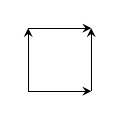
\begin{tikzpicture}[>=stealth,x=8mm,y=8mm]
\draw[->] (0,0) -- (1,0);
\draw[->] (0,1) -- (1,1);
\draw[->] (0,0) -- (0,1);
\draw[->] (1,0) -- (1,1);
\end{tikzpicture}}\endgroup}
\end{GelfandAdjacentEvidence}
\begin{GelfandAdjacentEvidence}{GELFAND-P001405}{4}


[In the right margin:]
\SourceFigure{GELFAND-P001405}{margin-arrows}{%
Here
\(\begin{matrix}\longrightarrow\\\longrightarrow\end{matrix}\)
horizontal morphisms,\par
\(\uparrow\,\uparrow\) vertical morphisms\par
(their sources and targets are 1-morphisms)}
\end{GelfandAdjacentEvidence}
\begin{GelfandAdjacentEvidence}{GELFAND-P001405}{5}


One can compose:

\SourceFigure{GELFAND-P001405}{composable-arrow-pairs}{%
\begin{tabular}{@{}r@{\enspace}l@{\quad}l@{}}
1)&\(\longrightarrow\;\longrightarrow\)&2 horizontal morphisms\\
2)&\(\begin{matrix}\uparrow\\\uparrow\end{matrix}\)&2 vertical morphisms
\end{tabular}}
\end{GelfandAdjacentEvidence}
\begin{GelfandAdjacentEvidence}{GELFAND-P001405}{6}


3) squares are multiplied in two ways

\SourceFigure{GELFAND-P001405}{square-composition}{%
\begingroup\color{black}\GelfandFitDiagram{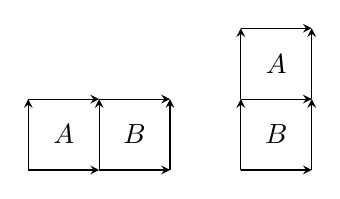
\begin{tikzpicture}[>=stealth,x=9mm,y=9mm]
\draw[->] (0,0) -- (1,0);
\draw[->] (1,0) -- (2,0);
\draw[->] (0,1) -- (1,1);
\draw[->] (1,1) -- (2,1);
\draw[->] (0,0) -- (0,1);
\draw[->] (1,0) -- (1,1);
\draw[->] (2,0) -- (2,1);
\node at (.5,.5) {\(A\)};
\node at (1.5,.5) {\(B\)};
\draw[->] (3,0) -- (4,0);
\draw[->] (3,1) -- (4,1);
\draw[->] (3,2) -- (4,2);
\draw[->] (3,0) -- (3,1);
\draw[->] (3,1) -- (3,2);
\draw[->] (4,0) -- (4,1);
\draw[->] (4,1) -- (4,2);
\node at (3.5,1.5) {\(A\)};
\node at (3.5,.5) {\(B\)};
\end{tikzpicture}}\endgroup}
\end{GelfandAdjacentEvidence}


(see Gabriel's book)


\Needspace{7\baselineskip}
\begin{GelfandAdjacentEvidence}{GELFAND-P001406}{1}
\SourcePage{GELFAND-P001406}{33}

\uline{Main nontrivial axiom}: 2-dimensional associativity

(1)
\SourceFigure{GELFAND-P001406}{interchange-diagram}{%
\begingroup\color{black}\GelfandFitDiagram{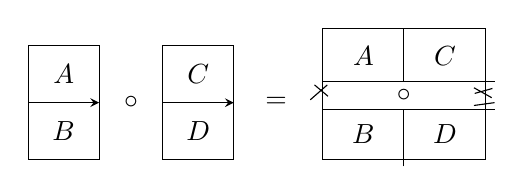
\begin{tikzpicture}[>=stealth,x=9mm,y=9mm]
  \draw (0,0) rectangle (1,1.6);
  \draw[->] (0,.8) -- (1,.8);
  \node at (.5,1.2) {\(A\)};
  \node at (.5,.4) {\(B\)};
  \node at (1.45,.8) {\(\circ\)};
  \draw (1.9,0) rectangle (2.9,1.6);
  \draw[->] (1.9,.8) -- (2.9,.8);
  \node at (2.4,1.2) {\(C\)};
  \node at (2.4,.4) {\(D\)};
  \node at (3.5,.8) {\(=\)};
  \draw (4.15,0) rectangle (6.45,1.85);
  \draw (4.15,.7) -- (6.58,.7);
  \draw (4.15,1.1) -- (6.58,1.1);
  \draw (5.3,-.1) -- (5.3,.7) (5.3,1.1) -- (5.3,1.85);
  \node at (4.73,1.46) {\(A\)};
  \node at (5.88,1.46) {\(C\)};
  \node at (4.73,.35) {\(B\)};
  \node at (5.88,.35) {\(D\)};
  \node at (5.3,.9) {\(\circ\)};
  \draw (3.98,.84) -- (4.22,1.05) (4.04,1.05) -- (4.23,.89);
  \draw (6.29,1.01) -- (6.54,.87) (6.3,.93) -- (6.55,1);
  \draw (6.29,.76) -- (6.58,.8);
\end{tikzpicture}}\endgroup
\par{\small The reading \(D\) is tentative. The strokes at the ends of the band on the right leave the arrows uncertain.}}
\end{GelfandAdjacentEvidence}
\begin{GelfandAdjacentEvidence}{GELFAND-P001406}{2}


\uline{Example where}
[crossed out: illegible]
\uline{ax. fails}
[crossed out: possibly an earlier «(1)»\textsuperscript{?}]
\uline{(1)}

\Incomplete{GELFAND-P001406}{example-cancel-left}{illegible}
\end{GelfandAdjacentEvidence}
\begin{GelfandAdjacentEvidence}{GELFAND-P001406}{3}

\Unclear{GELFAND-P001406}{example-cancel-right}{possibly an earlier «(1)»}
\end{GelfandAdjacentEvidence}
\begin{GelfandAdjacentEvidence}{GELFAND-P001406}{4}



\uline{Tensors:}

\SourceFigure{GELFAND-P001406}{tensor-horizontal}{%
\begingroup\color{black}\GelfandFitDiagram{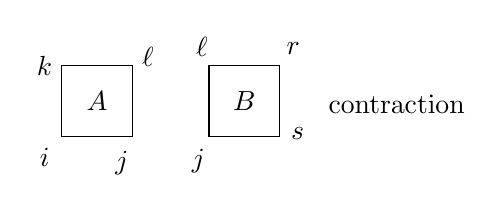
\begin{tikzpicture}[x=9mm,y=9mm]
  \draw (0,0) rectangle (1,1);
  \node at (.5,.5) {\(A\)};
  \node at (-.24,1) {\(k\)};
  \node at (1.22,1.13) {\(\ell\)};
  \node at (-.24,-.3) {\(i\)};
  \node at (.85,-.37) {\(j\)};
  \draw (2.08,0) rectangle (3.08,1);
  \node at (2.58,.5) {\(B\)};
  \node at (1.98,1.27) {\(\ell\)};
  \node at (3.27,1.24) {\(r\)};
  \node at (1.93,-.34) {\(j\)};
  \node at (3.33,.04) {\(s\)};
  \node[anchor=west] at (3.63,.45) {contraction};
\end{tikzpicture}}\endgroup}
\end{GelfandAdjacentEvidence}
\begin{GelfandAdjacentEvidence}{GELFAND-P001406}{5}


\[
(AB)_{ik}^{rs}=\sum A_{ij}^{k\ell} B_{js}^{\ell r}
\]
\EvidenceBlock{GELFAND-P001406}{tensor-indices}{On the left, \(i,k\) are subscripts and \(r,s\) are superscripts. The indices on the right follow the corner labels in the drawings of \(A\) and \(B\).}{Manuscript notation.}
\end{GelfandAdjacentEvidence}
\begin{GelfandAdjacentEvidence}{GELFAND-P001406}{6}


\SourceFigure{GELFAND-P001406}{tensor-vertical}{%
\begingroup\color{black}\GelfandFitDiagram{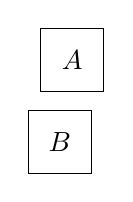
\begin{tikzpicture}[x=8mm,y=8mm]
  \draw (0,1.3) rectangle (1,2.3);
  \node at (.5,1.8) {\(A\)};
  \draw (-.2,0) rectangle (.8,1);
  \node at (.3,.5) {\(B\)};
\end{tikzpicture}}\endgroup}
\end{GelfandAdjacentEvidence}
\begin{GelfandAdjacentEvidence}{GELFAND-P001406}{7}


Axiom (1) will fail.

\uline{Another def.} (\uline{M. Kontsevich}) (competing)

\SourceFigure{GELFAND-P001406}{parallel-morphisms}{%
\begingroup\color{black}\GelfandFitDiagram{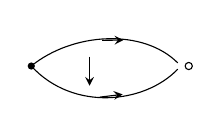
\begin{tikzpicture}[>=stealth,x=10mm,y=10mm]
  \fill (0,0) circle (1.3pt);
  \draw (2,0) circle (1.3pt);
  \draw (0,0) .. controls (.53,.43) and (1.42,.48) .. (1.86,.04);
  \draw[->] (.9,.326) -- (1.17,.33);
  \draw (0,0) .. controls (.53,-.58) and (1.44,-.48) .. (1.86,-.04);
  \draw[->] (.87,-.395) -- (1.16,-.36);
  \draw[->] (.74,.12) -- (.74,-.25);
\end{tikzpicture}}\endgroup
\par morphisms between morphisms with the same endpoints.}
\end{GelfandAdjacentEvidence}
\begin{GelfandAdjacentEvidence}{GELFAND-P001406}{8}


\uline{Example:} \(Cat\) (the category of categories. There is a morphism of functors)

This is a special case of the preceding one (contract the vertical arrows).

\uline{I. M. G.}

\SourceFigure{GELFAND-P001406}{boundary-diagram}{%
\begingroup\color{black}\GelfandFitDiagram{\begin{tikzpicture}[>=stealth,x=11mm,y=11mm]
  \draw[thick] (0,0) rectangle (1.55,1.24);
  \draw[->] (.05,.94) -- (1.43,1.03);
  \draw[->] (.08,.16) -- (1.48,.29);
  \draw[->] (.18,.03) -- (.29,1.15);
  \draw[->] (.33,.03) -- (.47,1.16);
  \node at (1,.59) {\(\Delta u=0\)};
  \node[anchor=east] at (-.1,.22) {\(u\) and \(\dfrac{\partial u}{\partial n}\)};
  \node[anchor=east] at (-.55,.86) {sv.\textsuperscript{?}};
\end{tikzpicture}}\endgroup
\par boundary conditions
\par{\small The open stroke and tall loop above \(u\) tentatively read «sv.».}}
\end{GelfandAdjacentEvidence}


Request to Keldysh, Chentsov, and Gelfand

\uuline{K.} Higher fundamental groups.
\(X_0\subset X_1\subset X\) is a topological space

objects are points \(x\in X_0\)

morph.
\(\bigl(\underset{\text{interval}}{I},\partial I\bigr)
\longrightarrow(X_1,X_0)\)
\qquad homotopic \((\bmod\,\partial I)\) are regarded as equivalent.

bimorphisms
\((I^2,\partial I^2)\longrightarrow(X,X_1)\)
\qquad \((\bmod\,\text{\uline{homotopy}})\)


\Needspace{7\baselineskip}
\begin{GelfandAdjacentEvidence}{GELFAND-P001407}{1}
\SourcePage{GELFAND-P001407}{44}

\uuline{23/XI-87}\qquad \uline{Gelfand seminar.}

\uline{Beilinson} (continued)

\uline{Derived categories.}

(1) \uline{Lemma:}
\SourceFigure{GELFAND-P001407}{lemma-roofs}{%
\begingroup\color{black}\GelfandFitDiagram{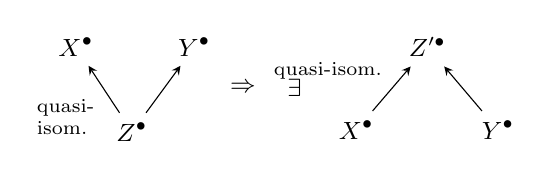
\begin{tikzpicture}[>=stealth,x=8mm,y=8mm,font=\small]
  \node (x) at (0,1.35) {\(X^\bullet\)};
  \node (y) at (1.88,1.35) {\(Y^\bullet\)};
  \node (z) at (.89,0) {\(Z^\bullet\)};
  \draw[->] (z) -- (x) node[midway,below left,align=left,font=\scriptsize] {quasi-\\isom.};
  \draw[->] (z) -- (y);
  \node at (2.65,.7) {\(\Rightarrow\)};
  \node at (3.47,.7) {\(\exists\)};
  \node (xx) at (4.45,.03) {\(X^\bullet\)};
  \node (yy) at (6.7,.03) {\(Y^\bullet\)};
  \node (zz) at (5.58,1.35) {\(Z'^\bullet\)};
  \draw[->] (xx) -- (zz) node[midway,above left,font=\scriptsize] {quasi-isom.};
  \draw[->] (yy) -- (zz);
\end{tikzpicture}}\endgroup}
\end{GelfandAdjacentEvidence}
\begin{GelfandAdjacentEvidence}{GELFAND-P001407}{2}


The lemma is proved using the mapping cone construction.

\uline{Reminder:}

\(\mathcal A\) is an ab. category
\SourceFigure{GELFAND-P001407}{category-sequence}{%
\(\begin{array}{@{}ccccc@{}}
C(\mathcal A)&\longrightarrow&K(\mathcal A)&\longrightarrow&D(\mathcal A)\\
\text{\scriptsize complexes}&&
\substack{\text{homotopy}\\\text{category}\\\text{of complexes}}&&
\substack{\text{derived}\\\text{category}}
\end{array}\)}
\end{GelfandAdjacentEvidence}
\begin{GelfandAdjacentEvidence}{GELFAND-P001407}{3}

[At right:] (the objects are complexes throughout)

\(f:X^\bullet\to Y^\bullet\) is homotopic to \(0\) if
\(\exists g^i:X^i\to Y^{i-1}\),
\[
f^i=dg^i+g^{i+1}d.
\]

\(D(\mathcal A)\) is \(K(\mathcal A)\) with the following inverted
\uline{quasi-isomorphisms}
(morphisms inducing an isomorphism of cohomology)

A morphism from \(X^\bullet\) to \(Y^\bullet\) is a diagram in \(K(\mathcal A)\)

(2)
\SourceFigure{GELFAND-P001407}{morphism-roof}{%
\begingroup\color{black}\GelfandFitDiagram{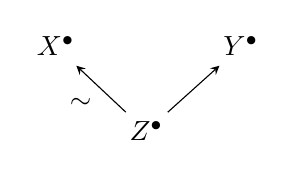
\begin{tikzpicture}[>=stealth,x=10mm,y=9mm]
  \node (x) at (0,1.2) {\(X^\bullet\)};
  \node (y) at (2.35,1.2) {\(Y^\bullet\)};
  \node (z) at (1.15,0) {\(Z^\bullet\)};
  \draw[->] (z) -- (x) node[midway,below left] {\(\sim\)};
  \draw[->] (z) -- (y);
\end{tikzpicture}}\endgroup}
\end{GelfandAdjacentEvidence}
\begin{GelfandAdjacentEvidence}{GELFAND-P001407}{4}

(the left arrow is a quasi-isomorphism)

more precisely, an equivalence class of such diagrams. Diagram (2) is equivalent to the diagram obtained using any quasi-isomorphism
\(\chi:Z'^\bullet\to Z^\bullet\)

(3)
\SourceFigure{GELFAND-P001407}{refinement-roofs}{%
\begingroup\color{black}\GelfandFitDiagram{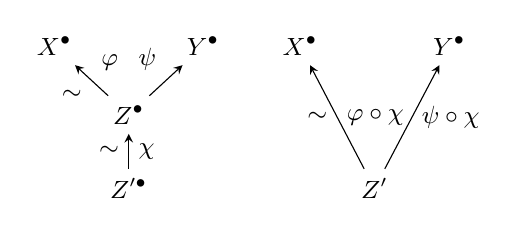
\begin{tikzpicture}[>=stealth,x=8mm,y=8mm,font=\small]
  \node (x) at (0,1.93) {\(X^\bullet\)};
  \node (y) at (2.36,1.93) {\(Y^\bullet\)};
  \node (z) at (1.18,.84) {\(Z^\bullet\)};
  \node (zp) at (1.18,-.33) {\(Z'^\bullet\)};
  \draw[->] (z) -- (x) node[midway,above right] {\(\varphi\)}
    node[midway,below left] {\(\sim\)};
  \draw[->] (z) -- (y) node[midway,above left] {\(\psi\)};
  \draw[->] (zp) -- (z) node[midway,right] {\(\chi\)}
    node[midway,left] {\(\sim\)};
  \node (xx) at (3.9,1.93) {\(X^\bullet\)};
  \node (yy) at (6.27,1.93) {\(Y^\bullet\)};
  \node (zz) at (5.08,-.33) {\(Z'\)};
  \draw[->] (zz) -- (xx) node[midway,right] {\(\varphi\circ\chi\)}
    node[midway,left] {\(\sim\)};
  \draw[->] (zz) -- (yy) node[midway,right] {\(\psi\circ\chi\)};
\end{tikzpicture}}\endgroup}
\end{GelfandAdjacentEvidence}
\begin{GelfandAdjacentEvidence}{GELFAND-P001407}{5}


(this relation extends to the smallest equivalence relation containing it)

The cone of a morphism and exact triangles were defined [crossed out: illegible] already.
\Unclear{GELFAND-P001407}{last-line-cancellation}{The short crossed-out passage before «already» is illegible.}
\end{GelfandAdjacentEvidence}



\Needspace{7\baselineskip}
\begin{GelfandAdjacentEvidence}{GELFAND-P001408}{1}
\SourcePage{GELFAND-P001408}{unlabelled}

\uuline{I. Zakharevich}
[crossed out: illegible]
\uline{Improvisation on chaos.}

\Incomplete{GELFAND-P001408}{cancelled-title}{illegible}
\end{GelfandAdjacentEvidence}
\begin{GelfandAdjacentEvidence}{GELFAND-P001408}{2}



\Unclear{GELFAND-P001408}{title-preposition}{The preposition in the title probably reads «o» (on). The open stroke also resembles «s».}
\end{GelfandAdjacentEvidence}
\begin{GelfandAdjacentEvidence}{GELFAND-P001408}{3}


\uline{Examples}

\(1^\circ\). Apparently there is a morphism from one example to the other.
\[
M=(\mathbb{Z}/2\mathbb{Z})^{\mathbb{Z}}
\qquad\text{(sequences infinite in both directions)}
\]
\(T:M\to M\). \(M\) has the standard topology (a Cantor set).
\[
a_i\to a_{i-1}\qquad\text{(shift transformation, Bernoulli transformation)}
\]
Consider the iterates \(T^N\).

There is a measure on \(M\). The baker’s transformation coincides with this
[inserted above the line: (up to a set of measure \(0\))]
[crossed out: continuation on two lines].
\Unclear{GELFAND-P001408}{baker-cancellations}{The upper line appears to read «if one takes», the lower «not \(\mathbb{Z}\), instead of \(\mathbb{Z}\)».}
\end{GelfandAdjacentEvidence}
\begin{GelfandAdjacentEvidence}{GELFAND-P001408}{4}


\SourceFigure{GELFAND-P001408}{baker-axes}{%
\begingroup\color{black}\GelfandFitDiagram{\begin{tikzpicture}[>=stealth,x=24mm,y=24mm,font=\small]
  \draw[->] (0,0) -- (2.13,0);
  \draw[->] (0,0) -- (0,1.32);
  \draw (0,1) -- (1,1) -- (1,0);
  \draw (2.02,0) -- (2.02,.51);
  \draw[dashed] (.03,.49) -- (2.07,.54);
  \foreach \x in {.08,.3,.68,1.1,1.42,1.72} {
    \draw[thin] (\x,.12) -- ++(.14,.22);
  }
  \draw[->] (1.39,.34) .. controls (1.52,.81) and (1.24,.88) .. (.58,.78);
  \node[below left] at (0,0) {\(0\)};
  \node[left] at (0,1) {\(1\)};
  \node[below] at (1,0) {\(1\)};
\end{tikzpicture}}\endgroup}
\end{GelfandAdjacentEvidence}
\begin{GelfandAdjacentEvidence}{GELFAND-P001408}{5}


\SourceFigure{GELFAND-P001408}{baker-sequence}{%
\begingroup\color{black}\GelfandFitDiagram{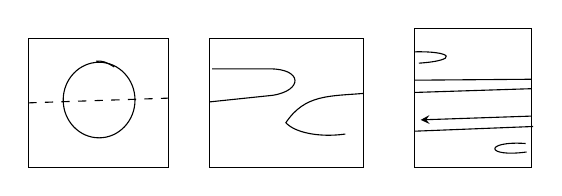
\begin{tikzpicture}[>=stealth,x=12mm,y=12mm]
  \draw (0,0) rectangle (1.48,1.36);
  \draw (.75,.71) ellipse (.38 and .4);
  \draw[dashed] (0,.68) -- (1.48,.73);
  \draw (.72,1.12) .. controls (.78,1.13) and (.83,1.11) .. (.91,1.06);
  \begin{scope}[xshift=23mm]
    \draw (0,0) rectangle (1.63,1.36);
    \draw (.03,1.04) -- (.64,1.04)
      .. controls (.99,1.04) and (.99,.81) .. (.67,.76)
      -- (0,.69);
    \draw (1.63,.78) .. controls (1.27,.75) and (1.01,.77) .. (.81,.47)
      .. controls (.9,.37) and (1.15,.31) .. (1.44,.35);
  \end{scope}
  \begin{scope}[xshift=49mm]
    \draw (0,0) rectangle (1.24,1.47);
    \draw (0,1.22) .. controls (.41,1.23) and (.48,1.13) .. (.05,1.1);
    \draw (0,.92) -- (1.24,.93) (0,.79) -- (1.24,.83);
    \draw[<-] (.07,.5) -- (1.24,.54);
    \draw (0,.38) -- (1.26,.43);
    \draw (1.18,.25) .. controls (.74,.28) and (.75,.1) .. (1.19,.16);
  \end{scope}
\end{tikzpicture}}\endgroup
\par and so on.
\par{\small The small strokes on the curves in the first and third drawings leave their direction uncertain.}}
\end{GelfandAdjacentEvidence}
\begin{GelfandAdjacentEvidence}{GELFAND-P001408}{6}


\uline{Correspondence}: write the coordinates of a point of the square in binary and take one digit to the left, the other to the right.

In what sense is this chaos

Consider \(T^k x,\ k\le 0\) — suppose this is known (to within \(1\) mm).
\[
T^k x,\qquad k>0
\]
In a finite time all this information will be lost.

\(2^\circ\). \uline{Hyperbolic transformation}: geodesic flows on manifolds of negative curvature.
\EvidenceBlock{GELFAND-P001408}{manifold-abbreviation}{The manuscript abbreviation is «mn-ziiakh» (manifolds).}{Manuscript notation.}
\end{GelfandAdjacentEvidence}
\begin{GelfandAdjacentEvidence}{GELFAND-P001408}{7}


\SourceFigure{GELFAND-P001408}{hyperbolic-surface}{%
\begingroup\color{black}\GelfandFitDiagram{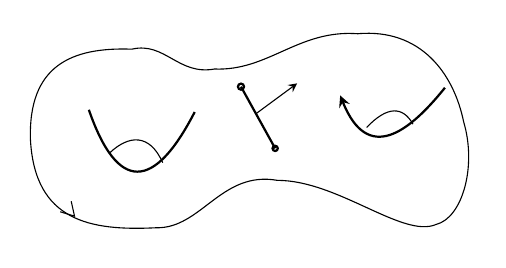
\begin{tikzpicture}[>=stealth,x=14mm,y=14mm]
  \draw (0,.8) .. controls (-.02,1.47) and (.37,1.64) .. (.92,1.62)
    .. controls (1.22,1.69) and (1.34,1.38) .. (1.67,1.44)
    .. controls (2.16,1.42) and (2.43,1.8) .. (2.97,1.76)
    .. controls (3.54,1.81) and (3.84,1.4) .. (3.93,.96)
    .. controls (4.05,.56) and (3.92,.09) .. (3.68,.03)
    .. controls (3.38,-.1) and (2.79,.43) .. (2.24,.43)
    .. controls (1.73,.52) and (1.55,-.01) .. (1.14,0)
    .. controls (.54,-.03) and (.04,.06) .. (0,.8);
  \draw[thick] (.53,1.07) .. controls (.79,.32) and (1.12,.33) .. (1.49,1.05);
  \draw (.72,.68) .. controls (.89,.84) and (1.08,.86) .. (1.2,.59);
  \draw (.37,.24) -- (.4,.105) -- (.27,.145);
  \draw[thick] (1.91,1.28) -- (2.22,.72);
  \draw[->] (2.04,1.03) -- (2.42,1.31);
  \draw[thick] (1.91,1.28) circle (1.1pt) (2.22,.72) circle (.95pt);
  \draw[thick,<-] (2.81,1.2) .. controls (3.06,.58) and (3.43,.86) .. (3.76,1.27);
  \draw (3.05,.91) .. controls (3.24,1.11) and (3.38,1.1) .. (3.47,.94);
\end{tikzpicture}}\endgroup
\par{\small The middle branch points up and right. The stroke near the left edge of the outline and the small marks on the middle segment are uncertain.}}
\end{GelfandAdjacentEvidence}



\Needspace{7\baselineskip}
\begin{GelfandAdjacentEvidence}{GELFAND-P001409}{1}
\SourcePage{GELFAND-P001409}{45}

\uuline{G. Margulis.}\qquad \uline{Iterations of maps of the complex plane.}

Consider the transformation \(z\to P(z)\), \(P\) is a polynomial

(more generally, a rational function)

\(\deg P=1\) [crossed out: illegible] uninteresting case
\Incomplete{GELFAND-P001409}{degree-one-cancellation}{The short passage after \(\deg P=1\) is illegible.}
\end{GelfandAdjacentEvidence}
\begin{GelfandAdjacentEvidence}{GELFAND-P001409}{2}


\begin{equation*}
z\mapsto az+b \tag{1}
\end{equation*}

\uline{Iterations}:
\[
z_{i+1}=P(z_i)
\]
\(\lvert a\rvert>1\Rightarrow\) one fixed point.

\(\lvert a\rvert=1\Rightarrow\) everything splits into invariant circles on which the map is a rotation.
\EvidenceBlock{GELFAND-P001409}{unit-modulus-claim}{The manuscript reads \(\lvert a\rvert=1\).}{Manuscript notation.}
\end{GelfandAdjacentEvidence}
\begin{GelfandAdjacentEvidence}{GELFAND-P001409}{3}


\SourceFigure{GELFAND-P001409}{invariant-circles}{%
\begingroup\color{black}\GelfandFitDiagram{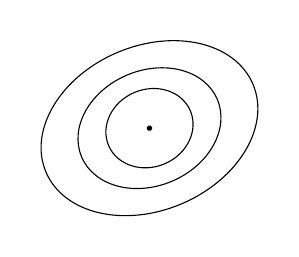
\begin{tikzpicture}[x=12mm,y=12mm,rotate=23]
  \draw (0,0) ellipse (1.19 and .87);
  \draw (0,0) ellipse (.78 and .61);
  \draw (0,0) ellipse (.47 and .41);
  \fill (0,0) circle (1pt);
\end{tikzpicture}}\endgroup}
\end{GelfandAdjacentEvidence}
\begin{GelfandAdjacentEvidence}{GELFAND-P001409}{4}


\uuline{I. M. G.}: 1) the question of when a transformation of the circle is diffeomorphically conjugate to a rotation is nontrivial. Denjoy, Arnold, Herman.

2) What is a representation of an infinite discrete group?

There is no satisfactory answer.

Von Neumann’s theorem is unaesthetic.

Chaos arises on the circle.

\uline{Conjecture}: if one works with sets of intermediate Hausdorff dimension, some of the classical theory will be recovered!!

\uline{Question for school students}: cover the \(n\)th rational number with an interval of length \(\varepsilon/2^n\). Give an example of a number that will remain uncovered.

\uline{Problem}: find the Hausdorff dimension of the perfect Cantor set.

\tikz[baseline=(emphasis.base)]\node[draw,circle,inner sep=2pt] (emphasis) {!};
\uuline{Problem}. \uwave{Construct a theory of representations of discrete groups on functions on sets of intermediate Hausdorff dimension.}

To begin, look at physics, string theory and so on.

\uuline{G. M.}:
\(z\to z^2\)
\qquad \(\lvert z\rvert=1\) maps to itself

\SourceFigure{GELFAND-P001409}{squaring-dynamics}{%
\begingroup\color{black}\GelfandFitDiagram{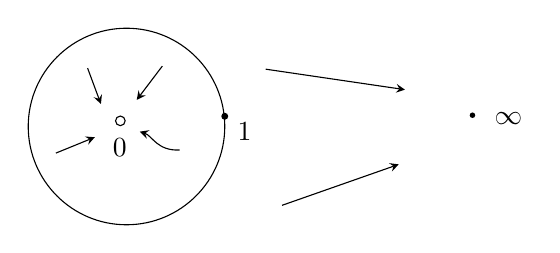
\begin{tikzpicture}[>=stealth,x=13mm,y=13mm]
  \draw (0,0) circle (.96);
  \draw (-.06,.055) circle (.047);
  \node[below] at (-.065,-.025) {\(0\)};
  \fill (.96,.1) circle (1.25pt);
  \node[right] at (.99,-.045) {\(1\)};
  \draw[->] (-.38,.57) -- (-.25,.22);
  \draw[->] (.35,.59) -- (.1,.26);
  \draw[->] (.52,-.23) .. controls (.3,-.24) and (.25,-.09) .. (.13,-.05);
  \draw[->] (-.69,-.26) -- (-.31,-.105);
  \draw[->] (1.36,.56) -- (2.72,.36);
  \draw[->] (1.52,-.77) -- (2.66,-.37);
  \fill (3.38,.11) circle (1pt);
  \node[right] at (3.5,.08) {\(\infty\)};
\end{tikzpicture}}\endgroup}
\end{GelfandAdjacentEvidence}


on the circle, an analogue of the (one-sided) baker’s transformation


\Needspace{7\baselineskip}
\begin{GelfandAdjacentEvidence}{GELFAND-P001410}{1}
\SourcePage{GELFAND-P001410}{unlabelled}

\[
f_n=\underbrace{f\circ f\circ\cdots\circ f}_{n\ \text{times}}
\]

\uline{Def.}

\(U\) is a
[crossed out: set; inserted above the line: \uline{nbhd.}]
of normality if \(\left.f_n\right|_U\) is a compact set

(normal family of analytic functions)
\EvidenceBlock{GELFAND-P001410}{definition-cancellation}{«set» is crossed out and «nbhd.» is inserted above it.}{Manuscript notation.}
\end{GelfandAdjacentEvidence}
\begin{GelfandAdjacentEvidence}{GELFAND-P001410}{2}


[Crossed out on a short line by itself:]
\Incomplete{GELFAND-P001410}{isolated-cancellation}{illegible}
\end{GelfandAdjacentEvidence}
\begin{GelfandAdjacentEvidence}{GELFAND-P001410}{3}


\uline{Set of normality} [inserted above the line: \(X\)] consists of points \(x\),
for which \(\exists\) nbhd. \(U\) ---
[crossed out: illegible] a nbhd. of normality
\Incomplete{GELFAND-P001410}{normality-cancellation}{The crossed-out writing before «nbhd. of normality» is illegible.}
\end{GelfandAdjacentEvidence}
\begin{GelfandAdjacentEvidence}{GELFAND-P001410}{4}


[Under \uline{Set of normality}: (it is open)]

The complement of the set of normality is the \uwave{Julia set}.

(it is closed)

The set of normality can be empty

\[
X=X_1\cup\cdots\cup X_n\cup\cdots
\]
(connected components) of the set of normality

[crossed out below this caption: illegible]
\Incomplete{GELFAND-P001410}{components-cancellation}{Individual letters are visible below the caption, but the passage cannot be read as a whole.}
\end{GelfandAdjacentEvidence}
\begin{GelfandAdjacentEvidence}{GELFAND-P001410}{5}


\[
\begin{aligned}
f:(\text{connected comp.})&\to(\text{connected components})\\
X_i&\mapsto X_{j(i)}
\end{aligned}
\]

\uwave{Sullivan} proved that for the resulting [crossed out: illegible]
map of a discrete set (countable or finite)
\Incomplete{GELFAND-P001410}{sullivan-cancellation}{The crossed-out writing before «map» is illegible.}
\end{GelfandAdjacentEvidence}
\begin{GelfandAdjacentEvidence}{GELFAND-P001410}{6}


a) each orbit stabilizes,

b) the set of fixed points is finite.

\uline{Idea of the proof.} Suppose there is an infinite orbit

\SourceFigure{GELFAND-P001410}{orbit-diagram}{%
\begingroup\color{black}\GelfandFitDiagram{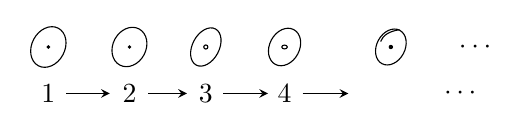
\begin{tikzpicture}[>=stealth,x=10mm,y=10mm]
  \foreach \x/\radiusX/\radiusY in {0/.21/.27,1.03/.21/.26,2/.17/.26,3/.19/.25,4.35/.18/.24} {
    \begin{scope}[shift={(\x,0)},rotate=-28]
      \draw (0,0) ellipse[x radius={\radiusX},y radius={\radiusY}];
    \end{scope}
  }
  \fill (0,0) circle (.7pt) (1.03,0) circle (.7pt) (4.35,0) circle (.8pt);
  \draw (2,0) circle (.75pt) (3,0) ellipse (1.0pt and .7pt);
  \draw (4.22,.07) .. controls (4.25,.15) and (4.33,.2) .. (4.46,.22);
  \node at (5.42,0) {\(\cdots\)};
  \foreach \x/\digit in {0/1,1.03/2,2/3,3/4} {
    \node at (\x,-.59) {\(\digit\)};
  }
  \foreach \from/\to in {.23/.78,1.27/1.76,2.22/2.79,3.23/3.81} {
    \draw[->] (\from,-.59) -- (\to,-.59);
  }
  \node at (5.23,-.59) {\(\cdots\)};
\end{tikzpicture}}\endgroup}
\end{GelfandAdjacentEvidence}
\begin{GelfandAdjacentEvidence}{GELFAND-P001410}{7}


Let us change the conformal [crossed out: possibly «transf.»] structure so that the transformation remains conformal.
\Unclear{GELFAND-P001410}{structure-cancellation}{The crossed-out abbreviation tentatively reads «preobr.» (transf.).}
\end{GelfandAdjacentEvidence}
\begin{GelfandAdjacentEvidence}{GELFAND-P001410}{8}


\uline{Problem:}

\SourceFigure{GELFAND-P001410}{circle-packing}{%
\begingroup\color{black}\GelfandFitDiagram{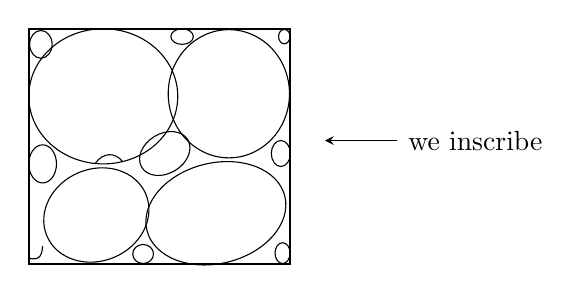
\begin{tikzpicture}[>=stealth,x=11mm,y=11mm]
  \draw[thick] (0,0) rectangle (3.02,2.72);
  \draw (.86,1.94) ellipse (.86 and .78);
  \draw (2.31,1.97) ellipse (.7 and .74);
  \draw[rotate around={23:(.78,.57)}] (.78,.57) ellipse (.62 and .53);
  \draw[rotate around={14:(2.16,.59)}] (2.16,.59) ellipse (.82 and .58);
  \draw[rotate around={31:(1.57,1.28)}] (1.57,1.28) ellipse (.31 and .23);
  \draw (.16,1.16) ellipse (.16 and .22);
  \draw (2.91,1.28) ellipse (.11 and .15);
  \draw (.14,2.54) ellipse (.13 and .16);
  \draw (1.77,2.63) ellipse (.13 and .09);
  \draw (2.95,2.63) ellipse (.066 and .083);
  \draw (1.32,.12) ellipse (.12 and .11);
  \draw (2.93,.13) ellipse (.087 and .12);
  \draw (0,.07) .. controls (.14,.04) and (.15,.12) .. (.16,.21) (.77,1.17) .. controls (.86,1.29) and (.99,1.30) .. (1.08,1.19);
  \draw[<-] (3.42,1.43) -- (4.25,1.43);
  \node[right] at (4.27,1.43) {we inscribe};
\end{tikzpicture}}\endgroup
\par{\small The contacts and some small arcs at the boundary are shown approximately.}}
\end{GelfandAdjacentEvidence}


1) Prove that the remainder has measure \(0\)

2) Prove that the remainder has Hausdorff dimension \(<2\).


\Needspace{7\baselineskip}
\begin{GelfandAdjacentEvidence}{GELFAND-P001411}{1}
\SourcePage{GELFAND-P001411}{46}

\uuline{I. M. Gelfand}. \uline{Matroids.}

In a \(K\)-dimensional space, consider \(n\) vectors.
Number them and list which are linearly dependent and which are not.

Giving this list defines a \uwave{matroid}.

What conditions apply to this list?

\uline{Example}:
[Crossed out: illegible]
\Incomplete{GELFAND-P001411}{example-cancelled}{The writing after «Example» is illegible.}
\end{GelfandAdjacentEvidence}
\begin{GelfandAdjacentEvidence}{GELFAND-P001411}{2}


\SourceFigure{GELFAND-P001411}{fano-diagram}{%
\begingroup\color{black}\GelfandFitDiagram{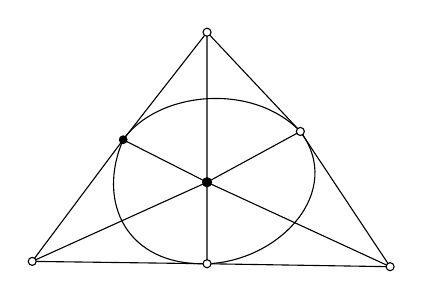
\begin{tikzpicture}[x=15mm,y=15mm]
  \coordinate (a) at (0,1.96);
  \coordinate (b) at (-1.48,.02);
  \coordinate (c) at (1.55,-.025);
  \coordinate (d) at (-.71,1.05);
  \coordinate (e) at (.79,1.12);
  \coordinate (f) at (0,0);
  \coordinate (g) at (0,.69);
  \draw (a)--(d)--(b)--(f)--(c)--(e)--cycle;
  \draw (a)--(g)--(f) (b)--(g)--(e) (d)--(g)--(c);
  \draw (d) .. controls (-.43,1.45) and (.37,1.55) .. (e)
    .. controls (1.17,.61) and (.61,.02) .. (f)
    .. controls (-.68,-.02) and (-.94,.52) .. (d);
  \foreach \point in {a,b,c,e,f} {
    \draw[fill=white] (\point) circle (1.45pt);
  }
  \fill (d) circle (1.6pt) (g) circle (1.85pt);
\end{tikzpicture}}\endgroup}
\end{GelfandAdjacentEvidence}
\begin{GelfandAdjacentEvidence}{GELFAND-P001411}{3}


If 3 points lie on one line, the vectors are linearly dependent.

The whole space is 3-dimensional (no 4 linearly independent vectors)

(1) \uline{Problem}: 1) prove that over \(\mathbb R\) and \(\mathbb C\)
there are no such vectors!

2) over \(\mathbb Z/2\mathbb Z\) there are such vectors.

(all the nonzero vectors of \((\mathbb Z/2\mathbb Z)^3\)!)

\uline{General} (\uline{unsolved problem}): which matroids are realizable
a) over \(\mathbb R\)
b) over \(\mathbb C\).?

\uwave{Solved problem}: which matroids are realizable over \(\forall\) fields?

\uline{In Rota’s book} e\textsuperscript{?}\ldots
[At right: see book\textsuperscript{?} by \uwave{Aigner} (?)]
there are 15 different equivalent definitions of a matroid.

\Unclear{GELFAND-P001411}{book-after-rota}{After «Rota» there is a curve resembling «e» (Cyrillic «э»), followed by dots. The curve joins the underlining.}
\end{GelfandAdjacentEvidence}
\begin{GelfandAdjacentEvidence}{GELFAND-P001411}{4}

\Unclear{GELFAND-P001411}{book-overwritten-noun}{The word after «see» has been overwritten and tentatively reads «книге» or «книжке» (book).}
\end{GelfandAdjacentEvidence}
\begin{GelfandAdjacentEvidence}{GELFAND-P001411}{5}


(2) \uline{Axioms.}

Certain subsets are singled out, \uwave{called bases}

\(B_1,B_2\) are 2 bases

\[
y\in B_2,\ y\notin B_1\Rightarrow\exists x\in B_1;\qquad
(B_1\setminus x)\cup y,\quad (B_2\setminus y)\cup x
\]
are bases [Crossed out: writing between the two expressions]
\Incomplete{GELFAND-P001411}{basis-exchange-cancelled}{The writing after \((B_1\setminus x)\cup y\) is crossed out and illegible.}
\end{GelfandAdjacentEvidence}
\begin{GelfandAdjacentEvidence}{GELFAND-P001411}{6}


\uwave{Exercise in linear algebra}: verify this for a set of vectors in a linear space.

(3) \uwave{Bimatroid}: consider a matrix. It defines 2 matroids, one by columns and one by rows

\(S\) and \(T\)

Another notion: list all the minors \(\ne0\)

Bimatroid: a collection of subsets with the same number of elements.

(4) [Crossed out: illegible] \uline{Problem}: give axioms for a bimatroid.
\Incomplete{GELFAND-P001411}{problem-four-cancelled}{The short passage before «Problem» is illegible.}
\end{GelfandAdjacentEvidence}



\Needspace{7\baselineskip}
\begin{GelfandAdjacentEvidence}{GELFAND-P001412}{1}
\SourcePage{GELFAND-P001412}{unlabelled}

(5) \uline{Problem}: how is the notion of a bimatroid from
[Crossed out: illegible] Gelfand–Serganova (UMN)
related to «Kuntom»\textsuperscript{?}
\Incomplete{GELFAND-P001412}{top-cancelled}{The crossed-out writing after “from” is illegible.}
\end{GelfandAdjacentEvidence}
\begin{GelfandAdjacentEvidence}{GELFAND-P001412}{2}

\Unclear{GELFAND-P001412}{knuth-name}{The surname tentatively reads «Kuntom». The rounded stroke before «t» is unclear. The name may refer to Knuth.}
\end{GelfandAdjacentEvidence}
\begin{GelfandAdjacentEvidence}{GELFAND-P001412}{3}


\uline{Problem}: prove that

\[
\begin{aligned}
\text{(6)}\quad [x_1,\ldots,x_d][y_1,\ldots,y_d]
 &= \sum(-1)^{d-i}[y_1,x_2,\ldots,x_d]\\
 &\qquad [y_1,\ldots,y_{i-1},x_i,y_{i+1},\ldots,y_d]
\end{aligned}
\]
\EvidenceBlock{GELFAND-P001412}{determinant-formula-source}{The sign \( (-1)^{d-i} \) and the indices \(y_1\), \(x_i\) follow the manuscript.}{Manuscript notation.}
\end{GelfandAdjacentEvidence}
\begin{GelfandAdjacentEvidence}{GELFAND-P001412}{4}


\([x_1,\ldots,x_d]\) is the determinant formed from the vectors.

(7) \uline{Remark}: if \([x_1,\ldots,x_d]\), \([y_1,\ldots,y_d]\)
are bases, then the right-hand side has a nonzero term, which gives the exchange axiom (3)
\EvidenceBlock{GELFAND-P001412}{basis-axiom-reference}{The reference (3) follows the manuscript.}{Manuscript notation.}
\end{GelfandAdjacentEvidence}
\begin{GelfandAdjacentEvidence}{GELFAND-P001412}{5}


(8) \uline{Problem} (tedious). Hilbert’s chain of syzygies:
\[
(\text{ring})\longmapsto
\underset{\text{— determinants}}{(\text{generators})}
\longmapsto (\text{relations among the generators})
\]
\Unclear{GELFAND-P001412}{overwritten-eight}{The visible numeral reads 8. The overwritten numeral is illegible.}
\end{GelfandAdjacentEvidence}
\begin{GelfandAdjacentEvidence}{GELFAND-P001412}{6}


(9) (\uline{Claim}: (6) gives all the relations among the generators)

(10) a) Write down the whole chain!

b) Discretize the entire chain (write down the combinatorial relations).

(11) \uline{Problem}. A bimatroid is a list of minors \(\longrightarrow\)
[Crossed out: illegible] 2 matroids (rows and columns)
\Incomplete{GELFAND-P001412}{problem-eleven-cancelled}{The crossed-out writing before “2 matroids” is illegible.}
\end{GelfandAdjacentEvidence}
\begin{GelfandAdjacentEvidence}{GELFAND-P001412}{7}


A bimatroid is constructed from 2 matroids

\SourceFigure{GELFAND-P001412}{basis-grid}{%
\begingroup\color{black}\GelfandFitDiagram{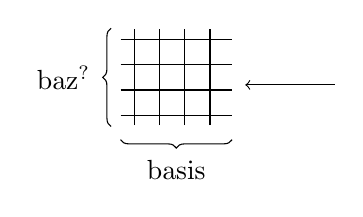
\begin{tikzpicture}[x=8mm,y=8mm]
  \foreach \x in {0,.4,.8,1.2} {
    \draw (\x,-.16) -- (\x,1.36);
  }
  \foreach \y in {0,.4,.8,1.2} {
    \draw (-.22,\y) -- (1.55,\y);
  }
  \draw[decorate,decoration={brace,amplitude=3pt}]
    (-.37,-.18) -- (-.37,1.38) node[midway,left=4pt]{baz\textsuperscript{?}};
  \draw[decorate,decoration={brace,amplitude=3pt}]
    (1.55,-.39) -- (-.22,-.39) node[midway,below=4pt]{basis};
  \draw[<-] (1.76,.48) -- (3.18,.48);
\end{tikzpicture}}\endgroup\par{\small The lower label reads «baza» (basis). The end of the label on the left is unclear.}}
\end{GelfandAdjacentEvidence}
\begin{GelfandAdjacentEvidence}{GELFAND-P001412}{8}


by def. \uwave{basis}.
\EvidenceBlock{GELFAND-P001412}{basis-construction-word}{The word after “by def.” is underlined and reads “basis.”}{Manuscript notation.}
\end{GelfandAdjacentEvidence}


But this is not necessary.

There is more information in a bimatroid.

What additional information is there in a bimatroid?

This is an important cohomological concept.

\uline{Remark}. Algebraic topology is a small island in the usual combinatorial technique.


\Needspace{7\baselineskip}
\SourcePage{GELFAND-P001413}{unlabelled}

\uuline{30/XI-87}\qquad \uline{Gelfand Seminar.}

\uline{I. M. Gelfand.} Problem: find the characters of the symmetric group.

(following Frobenius).

\uline{On the paper by} \uwave{Kerov}: «\uline{Realization of representations of the Hecke algebra} etc.»

Hint: these are characters of the symmetric group.

The Hecke algebra is the algebra with generators \(\{e_k\}\) [above the line: \(k=1,\ldots,N-1\)] and relations
\[
\text{(1)}\quad
\left\{\begin{aligned}
e_k e_{k+1}e_k-\tau e_k&=e_{k+1}e_ke_{k+1}-\tau e_{k+1}\\
e_{k+j}e_k&=e_ke_{k+j},\quad j\geqslant 2,\\
e_k^2&=e_k
\end{aligned}\right.
\]
Other generators
\[
\text{(2)}\quad \sigma_k=(q+1)e_k-1,\qquad \tau=\frac{q}{(q+1)^2}
\]
This algebra is denoted by \(H_N(q)\).

\uline{Exercise}: write down the relations for \(\sigma_k\).

(3) For \(q=1\) (or \(\tau=\frac14\)) we obtain the group algebra of the symmetric group.

(4) \uline{Problem}: \(\dim H_N(q)=N!\)

\begin{GelfandAdjacentEvidence}{GELFAND-P001413}{1}
[In the left margin: \textcircled{!}]
In the paper by Tipper and James

Proc. London Math. Soc.\qquad 1986, v. 52, p. 20--52

recommended!!

\EvidenceBlock{GELFAND-P001413}{citation-name}{The manuscript reads «Типпера» (Tipper). The cited publication gives R. Dipper.}{Manuscript notation.}
\end{GelfandAdjacentEvidence}
\begin{GelfandAdjacentEvidence}{GELFAND-P001413}{2}


it is proved that the representation theory of \(H_N(q)\) is analogous to the modular representation theory of the symmetric group.

This works even in the complex case (see the paper by Bernsh. — Gelf. — Gelf. on Verma modules).

Here it is assumed that \(q\ne\sqrt[m]{1}\)

\uwave{Construction of representations.}

Young diagram\quad \(\lambda=(\lambda_1,\lambda_2,\ldots,\lambda_k)\)

\SourceFigure{GELFAND-P001413}{young-diagram}{%
(5)\quad
\begingroup\color{black}\GelfandFitDiagram{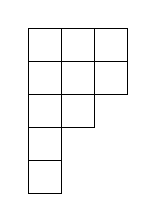
\begin{tikzpicture}[x=4.2mm,y=4.2mm,baseline=(current bounding box.center)]
  \draw (0,0)--(3,0)--(3,-2)--(2,-2)--(2,-3)--(1,-3)--(1,-5)--(0,-5)--cycle;
  \draw (1,0)--(1,-5) (2,0)--(2,-3);
  \draw (0,-1)--(3,-1) (0,-2)--(2,-2) (0,-3)--(1,-3) (0,-4)--(1,-4);
\end{tikzpicture}}\endgroup
\quad \(\begin{gathered}\sum\lambda_j=|\lambda|\\[4pt]\lambda_{i+1}\leqslant\lambda_i\end{gathered}\)}
\end{GelfandAdjacentEvidence}


(\(\lambda_i\) is the number of boxes in the \(i\)th column)

This corresponds to a conjugacy class of elements.


\Needspace{7\baselineskip}
\begin{GelfandAdjacentEvidence}{GELFAND-P001414}{1}
\SourcePage{GELFAND-P001414}{52}

Young tableau:
\[
\begin{aligned}
\text{(6)}\quad t=\{\lambda^{(k)}\}_{k=1}^{N}
&\quad\text{is a collection of diagrams in which}\\
|\lambda^{(k)}|&=k.
\end{aligned}
\]

The usual definition (a different one): the tableau is filled with the numbers \(1,2,\ldots,|\lambda|\), with
\[
\begin{matrix}\rightarrow\\\downarrow\end{matrix}
\quad\text{entries increasing in these directions}
\]

\SourceFigure{GELFAND-P001414}{tableau-large}{%
\begingroup\color{black}\GelfandFitDiagram{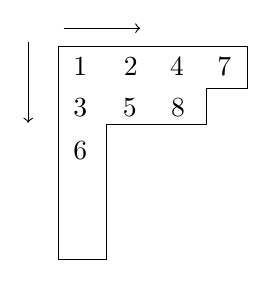
\begin{tikzpicture}[x=6mm,y=6mm]
  \draw (0,0)--(4,0)--(4,-.9)--(3.13,-.9)--(3.13,-1.66)
    --(1,-1.66)--(1,-4.52)--(0,-4.52)--cycle;
  \node at (.45,-.44) {\(1\)};
  \node at (1.52,-.44) {\(2\)};
  \node at (2.50,-.44) {\(4\)};
  \node at (3.50,-.44) {\(7\)};
  \node at (.45,-1.29) {\(3\)};
  \node at (1.50,-1.29) {\(5\)};
  \node at (2.52,-1.29) {\(8\)};
  \node at (.45,-2.22) {\(6\)};
  \draw[->] (.1,.38)--(1.72,.38);
  \draw[->] (-.65,.08)--(-.65,-1.62);
\end{tikzpicture}}\endgroup}
\end{GelfandAdjacentEvidence}
\begin{GelfandAdjacentEvidence}{GELFAND-P001414}{2}


In (6) they must increase

\SourceFigure{GELFAND-P001414}{tableau-growth}{%
\begingroup\color{black}\GelfandFitDiagram{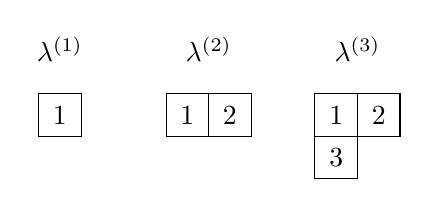
\begin{tikzpicture}[x=5.4mm,y=5.4mm]
  \node at (.5,1.05) {\(\lambda^{(1)}\)};
  \draw (0,0) rectangle (1,-1);
  \node at (.5,-.5) {\(1\)};
  \node at (4,1.05) {\(\lambda^{(2)}\)};
  \draw (3,0) rectangle (5,-1);
  \draw (4,0)--(4,-1);
  \node at (3.5,-.5) {\(1\)};
  \node at (4.5,-.5) {\(2\)};
  \node at (7.5,1.05) {\(\lambda^{(3)}\)};
  \draw (6.5,0)--(8.5,0)--(8.5,-1)--(7.5,-1)--(7.5,-2)--(6.5,-2)--cycle;
  \draw (7.5,0)--(7.5,-1) (6.5,-1)--(7.5,-1);
  \node at (7,-.5) {\(1\)};
  \node at (8,-.5) {\(2\)};
  \node at (7,-1.5) {\(3\)};
\end{tikzpicture}}\endgroup}
\end{GelfandAdjacentEvidence}
\begin{GelfandAdjacentEvidence}{GELFAND-P001414}{3}


\[
\text{(7)}\quad r_k(t)=(i_{k+1}-j_{k+1})-(i_k-j_k)
\]
point \(k\) has coordinates \((i_k,j_k)\)

For the diagram:
\[
\text{(8)}\quad h(\lambda)=r_\lambda+1
\]
\[
\text{(9)}\quad r_\lambda=\max_{t\in T(\lambda)}\max_{1\leq k\leq N}|r_k(t)|,
\]
where \(T(\lambda)\) is the set of tableaux constructed from the diagram \(\lambda\), i.e., of shape \(\lambda\).
\EvidenceBlock{GELFAND-P001414}{eq9-limit}{The manuscript writes \(1\leq k\leq N\).}{Manuscript notation.}
\end{GelfandAdjacentEvidence}
\begin{GelfandAdjacentEvidence}{GELFAND-P001414}{4}


Let \(s=(\mu^{(k)})_{k=1}^{N}\), \quad \(t=(\lambda^{(k)})_{k=1}^{N}\).

(10) \uline{Def.}\quad \(s\underset{n}{\approx}t\), if
\(\lambda^{(k)}=\mu^{(k)}\), \(k\ne n\)

\uline{Claim.}

(11) [Crossed out: if?] [Inserted above the line: Let] \(r_n(t)=\pm1\).
Then \(s\underset{n}{\approx}t\Rightarrow s=t\).
\Unclear{GELFAND-P001414}{eq11-cancelled-word}{The crossed-out word tentatively reads “if.” The insertion above the line reads “Let.”}
\end{GelfandAdjacentEvidence}
\begin{GelfandAdjacentEvidence}{GELFAND-P001414}{5}


(12) Let \(|r_n(t)|>1\). Then
\(\exists!\ s:\ s\underset{n}{\approx}t,\ s\ne t\).

\[
\text{(13)}\quad S_\lambda^{(k)}=\Vert S_{s,t}^{(k)}(\tau)\Vert_{s,t\in T(\lambda)}
\quad\text{is a matrix.}
\]
\Unclear{GELFAND-P001414}{eq13-terminal-mark}{Below and to the right of the matrix index is an unclear two-stroke mark with a curved tail, possibly \(q\) or a corrected comma.}
\end{GelfandAdjacentEvidence}
\begin{GelfandAdjacentEvidence}{GELFAND-P001414}{6}


\[
\text{(14)}\quad
S_{s,t}^{(k)}(\tau)=\bigl(W_{r_k(s)}(\tau)\ W_{r_k(t)}(\tau)\bigr)^{1/2}
\quad\text{if }s\underset{k}{\approx}t
\]
\Incomplete{GELFAND-P001414}{eq14-blotted-mark}{There is a blotted mark after the first factor.}
\end{GelfandAdjacentEvidence}
\begin{GelfandAdjacentEvidence}{GELFAND-P001414}{7}


[Crossed out: if \(s\underset{k}{\approx}t\)\textsuperscript{?}]
and \(S_{s,t}^{(k)}(\tau)=0\) otherwise.
\Unclear{GELFAND-P001414}{eq14-cancelled-condition}{The crossed-out condition tentatively reads “if \(s\underset{k}{\approx}t\).”}
\end{GelfandAdjacentEvidence}



\Needspace{7\baselineskip}
\begin{GelfandAdjacentEvidence}{GELFAND-P001415}{1}
\SourcePage{GELFAND-P001415}{unlabelled}

(15) \uline{Theorem}. Let \(\lambda\) be a diagram with \(N\) elements and
\(q\ne\sqrt[m]{1}\). Then \(S_{\lambda}^{(k)}\) give a representation of the Hecke algebra
(in the generators \(e_k\)).
\Unclear{GELFAND-P001415}{theorem-lambda}{The retraced subscript of \(S^{(k)}\) reads \(\lambda\). A crossing stroke merges with the retracing.}
\end{GelfandAdjacentEvidence}
\begin{GelfandAdjacentEvidence}{GELFAND-P001415}{2}


Let us construct the functions \(W\).

\(W_{-r}(\tau)\) for \(r=1,2,\ldots\) is determined from the relations
\[
\text{(16)}\quad W_{-(r+1)}(\tau)=1-\frac{\tau}{W_{-r}(\tau)},
\qquad r\geqslant0,
\]
[Crossed out: and for \(r\geqslant0\)\textsuperscript{?}]
\Unclear{GELFAND-P001415}{eq16-cancelled}{The two lower slanting strokes resemble those of \(\geqslant\) in (16). The cancellation crosses the upper stroke.}
\end{GelfandAdjacentEvidence}
\begin{GelfandAdjacentEvidence}{GELFAND-P001415}{3}

\[
\text{(17)}\quad W_r(\tau)=1-W_{-r}(\tau),\qquad r\geqslant0;
\]

Or:

\(W_{-r}(\tau)\) is determined [Crossed out: illegible] from its continued fraction expansion:
\Incomplete{GELFAND-P001415}{continued-fraction-cancelled-word}{The crossed-out word after “is determined” is illegible.}
\end{GelfandAdjacentEvidence}
\begin{GelfandAdjacentEvidence}{GELFAND-P001415}{4}


\[
\text{(18)}\quad \text{[Crossed out: }W_{-r}(\tau)=\text{]}\quad
1-\frac{\tau}{1-\dfrac{\tau}{1-\ldots}}
\]
\EvidenceBlock{GELFAND-P001415}{eq18-cancelled-expression}{The manuscript crosses out \(W_{-r}(\tau)=\) before the fraction.}{Manuscript notation.}
\end{GelfandAdjacentEvidence}
\begin{GelfandAdjacentEvidence}{GELFAND-P001415}{5}


There is an equation:
\[
\text{(19)}\quad W_r(\tau)W_{1-r}(\tau)=1.
\]
\EvidenceBlock{GELFAND-P001415}{eq19-right-hand-side}{The right-hand side of (19) reads \(1\).}{Manuscript notation.}
\end{GelfandAdjacentEvidence}
\begin{GelfandAdjacentEvidence}{GELFAND-P001415}{6}


General formula:
\[
\text{(20)}\quad W_r(\tau)=\frac{q(q^{r-1}-1)}{(q+1)(q^r-1)},\qquad r=1,2,\ldots
\]
\[
\text{(21)}\quad W_{-r}(\tau)=\frac{q^{r+1}-1}{(q+1)(q^r-1)}.
\]
\EvidenceBlock{GELFAND-P001415}{w-index}{The index of \(W\) and the corresponding letter in the exponents of \(q\) in (20) and (21) read \(r\).}{Manuscript notation.}
\end{GelfandAdjacentEvidence}
\begin{GelfandAdjacentEvidence}{GELFAND-P001415}{7}


(22) \uline{Problem}: find the characters of the Hecke algebra.

Consider
\[
\text{(23)}\quad
\frac{
 \begin{vmatrix}
 x_1^{i_1}&x_1^{i_2+1}&\ldots&x_1^{i_n+n-1}\\
 x_2^{i_1}&x_2^{i_2+1}&\ldots&x_2^{i_n+n-1}\\
 \ldots&\ldots&\ldots&\ldots\\
 x_n^{i_1}&\multicolumn{2}{c}{\ldots}&x_n^{i_n+n-1}
 \end{vmatrix}
}{
 \begin{vmatrix}
 1&x_1&x_1^2&\ldots&x_1^{n-1}\\
 1&x_2&x_2^2&&\\
 &&&&\\
 1&x_n&x_n^2&&x_n^{n-1}
 \end{vmatrix}
}
=\sum a(i,j)P_{j_1}P_{j_2}\ldots P_{j_n}
\]
\Unclear{GELFAND-P001415}{eq23-overwritten-exponents}{The first two rows of the final column visibly end in \(+n-1\). The subscripts on \(i\) are overwritten and may read \(n\) or \(4\). The last row clearly has \(n\).}
\end{GelfandAdjacentEvidence}



\Needspace{7\baselineskip}
\begin{GelfandAdjacentEvidence}{GELFAND-P001416}{1}
\SourcePage{GELFAND-P001416}{53}

\(j=(j_1,\ldots,j_n)\), \(P_j\) is a power sum.

Then

(24) \(a(i,j)\) is the character value [inserted above the line: of the symmetric group]
on an element with cycle lengths \(j_1,\ldots,j_n\)

(up to a simple constant)

For the symmetric group, see Macdonald’s book “Symmetric Functions and Hall Polynomials.”

\begin{center}
\rule{16mm}{.35pt}\enspace\(\cdot\)\enspace\rule{13mm}{.35pt}
\end{center}

\uline{Location of the poles of Ruelle’s zeta function.}

(Lindon Mayer (?))
\EvidenceBlock{GELFAND-P001416}{mayer-name}{The manuscript reads “Lindon Mayer (?)”, including the question mark. The cited article is by Dieter H. Mayer, \href{https://doi.org/10.1007/BF00420300}{\emph{On the location of poles of Ruelle’s zeta function}}, Lett. Math. Phys. 14 (1987), 105--115.}{Manuscript notation.}
\end{GelfandAdjacentEvidence}
\begin{GelfandAdjacentEvidence}{GELFAND-P001416}{2}


Letters in Math. Physics, \(14:2\), 1987.

\(I\) is an interval, \(T:I\to I\) is piecewise linear
\[
 I=\bigcup_j I_j,\qquad T(I_j)=I.
\]

\SourceFigure{GELFAND-P001416}{interval-graph}{%
\begingroup\color{black}\GelfandFitDiagram{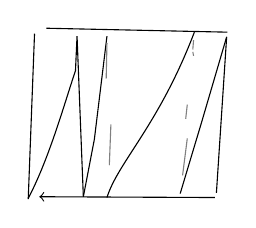
\begin{tikzpicture}[x=10mm,y=10mm]
  \draw (.10,0)--(.18,2.10) (.33,2.17)--(2.63,2.12)
    (2.62,2.06)--(2.49,.08);
  \draw[->] (2.47,.02)--(.24,.03);
  \draw (.10,.01) .. controls (.37,.52) and (.57,1.25) .. (.70,1.63)
    --(.72,2.07)--(.80,.03);
  \draw (.80,.03)--(.94,.76)--(1.10,2.07);
  \draw (1.10,.02) .. controls (1.24,.47) and (1.76,.94) .. (2.21,2.12);
  \draw (2.03,.07)--(2.30,.97)--(2.62,2.06);
  \draw[gray,thin] (1.10,1.98)--(1.09,1.53) (1.15,.95)--(1.13,.43)
    (2.20,2.02)--(2.19,1.90) (2.19,1.87)--(2.20,1.82) (2.12,1.20)--(2.10,1.02) (2.12,.77)--(2.06,.30);
\end{tikzpicture}}\endgroup
\par The attachment of the faint strokes to the branches and the exact locations of the breaks are unclear.}
\end{GelfandAdjacentEvidence}
\begin{GelfandAdjacentEvidence}{GELFAND-P001416}{3}


\[
\text{(1)}\quad \zeta_T(z,\varphi)=\frac{\det(1-zL_1)}{\det(1-zL_2)},
\]
where
\[
L_1f(z)=\varphi(z)\sum\frac{1}{\rho_j}f(\psi_j(z)),
\]
\[
L_2f(z)=\varphi(z)\sum f(\psi_j(z)),
\]
\(\psi_j\) are the local inverses of \(T\) on the interval \(I_j\), and \(\rho_j^{-1}\) is the slope.
\Unclear{GELFAND-P001416}{slope-letter}{The slope letter can be read as \(\rho_j\) or \(p_j\).}
\end{GelfandAdjacentEvidence}
\begin{GelfandAdjacentEvidence}{GELFAND-P001416}{4}


In the general case:
\[
\text{(2)}\quad
\zeta_T(z,\varphi)=\exp\left(
\sum_{n=1}^{\infty}\frac{z^n}{n}
\sum_{\xi\in\mathrm{Fix}\,T^n}
\prod_{k=0}^{n-1}\varphi(T^k x)\right)
\]
\EvidenceBlock{GELFAND-P001416}{eq2-variable}{The second sum is indexed by \(\xi\in\mathrm{Fix}\,T^n\). The product uses \(x\).}{Manuscript notation.}
\end{GelfandAdjacentEvidence}


\begin{center}
\rule{16mm}{.35pt}\enspace\(\cdot\)\enspace\rule{16mm}{.35pt}
\end{center}


\Needspace{7\baselineskip}
\begin{GelfandAdjacentEvidence}{GELFAND-P001417}{1}
\SourcePage{GELFAND-P001417}{unlabelled}

\uline{7/XII-87}\qquad \uline{Gelfand Seminar.}\qquad Some remarks on the paper by

\uline{D. Mayer}\qquad \uwave{Lett. in Math. Phys. 1987, 14:2}

\uline{On Ruelle’s \(\zeta\) function}

\(F\) is the set of spin values (finite).

We study spin configurations on a lattice
\[
(\xi_i),\qquad -\infty<i<\infty,\qquad \xi_i\in F.
\]

\(M\subseteq F\times F\) is the admissible set. We require
\[
\text{(1)}\quad (\xi_i,\xi_{i+1})\in M
\]

The simplest example of a Ruelle \(\zeta\) function is the Artin–Mazur \(\zeta\) function.

Consider the set of periodic configurations and their number:
\[
\text{(2)}\quad N_n=\#\{(\xi_i)\mid\mathcal T^n(\xi_i)=(\xi_i)\}
=\mathrm{Fix}\,\mathcal T^n,
\]
\EvidenceBlock{GELFAND-P001417}{eq2-fix}{The last term of (2) is written as \(\mathrm{Fix}\,\mathcal T^n\) without a cardinality sign.}{Manuscript notation.}
\end{GelfandAdjacentEvidence}
\begin{GelfandAdjacentEvidence}{GELFAND-P001417}{2}

where \(\mathcal T\) is the transformation on the space of sequences
\[
\mathcal T(\xi_i)=\xi_{i+1}
\]
(shift)

Ruelle’s \(\zeta\) function:
\[
\text{(3)}\quad
\zeta_{\mathcal T}(s)=\exp\left(\sum_{n=1}^{\infty}\frac{N_n}{n}s^n\right)
\]
the series converges for \(|s|<\dfrac{1}{|F|}\).

Does an analytic continuation exist? Consider the matrix
\Unclear{GELFAND-P001417}{continuation-question-overwriting}{The end of the first word and the initial letter of “analytic” are retraced in the manuscript.}
\end{GelfandAdjacentEvidence}

\[
\text{(4)}\quad T=(T_{\alpha\beta})=
\begin{cases}
1,&(\alpha,\beta)\in M,\\
0,&(\alpha,\beta)\notin M.
\end{cases}
\]

Then
\[
\text{(5)}\quad\zeta_{\mathcal T}(s)=\frac{1}{\det(1-sT)}
\]

This shows that \(\zeta_{\mathcal T}(s)\) is meromorphic.

The radius of convergence may exceed \(1/|F|\).

For the proof, observe that
\[
\text{(6)}\quad N_n=\mathrm{Tr}\,T^n.
\]


\Needspace{7\baselineskip}
\begin{GelfandAdjacentEvidence}{GELFAND-P001418}{1}
\SourcePage{GELFAND-P001418}{62}

\uwave{Remark by I. M. G.}: this resembles the work of Dynkin and Dmitriev:

consider a stochastic matrix \((p_{ik})\)
[inserted above the line: (a student’s)] (in the problem about basins this is the
[crossed-out sign: illegible] fraction of the water that flows from basin \(i\)to basin \(k\)).
\EvidenceBlock{GELFAND-P001418}{stochastic-insertion}{The manuscript inserts “(a student’s)” above the line.}{Manuscript notation.}
\end{GelfandAdjacentEvidence}
\begin{GelfandAdjacentEvidence}{GELFAND-P001418}{2}

\Incomplete{GELFAND-P001418}{basin-cancelled-sign}{The sign before “fraction” is crossed out and illegible.}
\end{GelfandAdjacentEvidence}
\begin{GelfandAdjacentEvidence}{GELFAND-P001418}{3}


\[
\underline{P}=(p_{ik}),\qquad \sum_k p_{ik}=1.
\]

This depends on the eigenvalues of \(P\).

a) The eigenvalues lie in the disk \(|\lambda|\leq1\),

b) \(1\) is an eigenvalue.

What region do the eigenvalues fill?

It is the interior of some algebraic curve.

They went about it the wrong way.

There is a whole set of eigenvalues!!

and one should plot the set of eigenvalues in \(\mathbb C^n\) — it ought to be a beautiful region (\uline{Problem}!!)

The projection onto a single axis can be complicated!

[Double line in the left margin.]
\uwave{In Ruelle’s problem it is \uline{interesting} to look at all the eigenvalues of the matrix}\quad \(T\).

\smallskip\hrule\smallskip

\uwave{Speaker.} Generalization of example (3)
\[
\text{(7)}\quad \zeta_{\mathcal T}(s,\varphi)=
 \exp\left(
 \sum_{n=1}^{\infty}\frac{s^n}{n}
 \sum_{\xi\in\mathrm{Fix}(\mathcal T^n)}
 \prod_{\ell=0}^{n}\varphi(\mathcal T^\ell\xi)
 \right)
\]
\EvidenceBlock{GELFAND-P001418}{eq7-upper-product-bound}{The upper limit of the product in (7) is written as \(n\).}{Manuscript notation.}
\end{GelfandAdjacentEvidence}
\begin{GelfandAdjacentEvidence}{GELFAND-P001418}{4}


Here
\[
 \underset{\substack{|\\\text{function}}}{\varphi}
 =\varphi(\xi_1,\ldots,\xi_k),\qquad \xi_j\in F
\]
(\(\varphi\) depends only on the first \(k\) values).

((3) is obtained for \(\varphi=1\))

(8) \uline{Claim.} \(\exists\) [Crossed out: operator?]
[inserted above the line: matrix] \(L\) (finite-dimensional), such that:
\Unclear{GELFAND-P001418}{matrix-insertion}{The crossed-out word tentatively reads “operator.” The insertion above it reads “matrix.”}
\end{GelfandAdjacentEvidence}
\begin{GelfandAdjacentEvidence}{GELFAND-P001418}{5}

\[
\text{(9)}\quad \zeta_{\mathcal T}(s,\varphi)=\frac{1}{\det(1-sL)}
\]

Specifically, consider
\[
F'=F^k;
\]
[Crossed out: \(F\times F\)\textsuperscript{?}]
\Incomplete{GELFAND-P001418}{before-m-prime-cancelled}{The crossed-out writing tentatively reads \(F\times F\). The crossing strokes obscure any superscripts or primes.}
\end{GelfandAdjacentEvidence}
\begin{GelfandAdjacentEvidence}{GELFAND-P001418}{6}

\[
M'\subset F'\times F'
\]
\[
\text{(10)}\quad
M'=\{(\xi_1,\ldots,\xi_k);(\xi_2,\ldots,\xi_{k+1})
 \mid(\xi_i,\xi_{i+1})\in M\}
\]
\Unclear{GELFAND-P001418}{eq10-overwritten-indices}{The corrected second tuple reads \(2\) and \(k+1\), and the condition reads \(i+1\). The earlier strokes beneath the retracing are illegible.}
\end{GelfandAdjacentEvidence}


Then take
\[
 \ell_{\alpha\beta}=
 \begin{cases}
 \varphi(\alpha),&(\alpha,\beta)\in M',\\
 0,&(\alpha,\beta)\notin M',
 \end{cases}
 \qquad L=(\ell_{\alpha\beta}).
\]


\Needspace{7\baselineskip}
\begin{GelfandAdjacentEvidence}{GELFAND-P001419}{1}
\SourcePage{GELFAND-P001419}{unlabelled}

\uwave{I. M. G.}

\uline{NB}: one needs to know the \(p\)-adic numbers

(be able to add, multiply, and divide them, [crossed out: illegible] and extract roots)
\Incomplete{GELFAND-P001419}{nb-cancelled-letter}{The mark after “divide” is crossed out and illegible.}
\end{GelfandAdjacentEvidence}
\begin{GelfandAdjacentEvidence}{GELFAND-P001419}{2}


\uuline{Beilinson A.}\qquad \uline{\(p\)-adic numbers and physics.}

\uline{On some of Manin’s \(p\)-adic ideas in physics}!
\Unclear{GELFAND-P001419}{heading-last-sign}{The last mark resembles “!” and may read “?”.}
\end{GelfandAdjacentEvidence}
\begin{GelfandAdjacentEvidence}{GELFAND-P001419}{3}


\(1^{\circ}\). Witten listened to the talk by Faltings with great interest and then bought all the books on number theory.
The only thing he understood from the talk was the formula
\EvidenceBlock{GELFAND-P001419}{faltings-name}{The manuscript spells the surname “Фалтингса” (Faltings).}{Manuscript notation.}
\end{GelfandAdjacentEvidence}
\begin{GelfandAdjacentEvidence}{GELFAND-P001419}{4}

\[
\text{(1)}\quad |a|_\infty\cdot|a|_2|a|_3\ldots=1,\qquad a\in\mathbb Q.
\]

For \(\dfrac12\) we have here:
\[
\frac12\cdot 2\cdot 1\ldots=1.
\]

There are 3 papers:

1) \uwave{Volovich}\qquad (in Russian)

2) \uwave{Yu. I. Manin}\qquad (in English)

3) \uwave{Witten} and someone else
\Unclear{GELFAND-P001419}{witten-list-final-sign}{An isolated illegible mark stands to the right of the third entry.}
\end{GelfandAdjacentEvidence}
\begin{GelfandAdjacentEvidence}{GELFAND-P001419}{5}


All 3 papers appeared in September.

\uwave{Witten’s text.}

Consider the functional equation for the Riemann \(\zeta\) function
\[
\begin{aligned}
\text{(2)}\quad\pi^{-s/2}\Gamma(s/2)\prod(1-p^{-s})^{-1}
&=\pi^{-(1-s)/2}\Gamma\left(\frac{1-s}{2}\right)
\prod(1-p^{-(1-s)})^{-1}.
\end{aligned}
\]
(analytic continuation is understood)

or (formally):
\[
\text{(3)}\quad
\frac{\pi^{-s+1}\Gamma(s/2)}{\Gamma\left(\dfrac{1-s}{2}\right)}
=\prod_p\frac{1-p^{-s}}{1-p^{s-1}}.
\]
\EvidenceBlock{GELFAND-P001419}{eq3-pi-exponent}{The exponent of \(\pi\) is written as \(-s+1\).}{Manuscript notation.}
\end{GelfandAdjacentEvidence}


On the left \(\approx\) the Veneziano–Witten amplitude for an open string [inserted above the line: (with momentum \(s\))].
On the right is a divergent expression, but what matters is that it is written as a product over the primes!


\Needspace{7\baselineskip}
\begin{GelfandAdjacentEvidence}{GELFAND-P001420}{1}
\SourcePage{GELFAND-P001420}{63}

\uwave{\(2^{\circ}\). On Manin’s work}

(1) \uline{Claim}: The Tamagawa measure \(=1\).

In more detail:
\[
\mathrm{SL}(n,\mathbb R)\supset\mathrm{SL}(n,\mathbb Z).
\]

On \(\mathrm{SL}(n,\mathbb R)\) there is an invariant
[inserted above “invariant”: «left»] measure (the standard one).
\Incomplete{GELFAND-P001420}{measure-tail}{A crossed-out mark is visible below the end of “measure.”}
\end{GelfandAdjacentEvidence}
\begin{GelfandAdjacentEvidence}{GELFAND-P001420}{2}


Normalize [crossed out: illegible] using the integer matrices.
\Incomplete{GELFAND-P001420}{normalization-cancelled}{The writing after “Normalize” is crossed out and illegible.}
\end{GelfandAdjacentEvidence}
\begin{GelfandAdjacentEvidence}{GELFAND-P001420}{3}

\[
\operatorname{vol}\bigl(\mathrm{SL}(n,\mathbb R)/\mathrm{SL}(n,\mathbb Z)\bigr)-?
\]

[In the right margin:]
(it is constructed from the standard basis in the Lie algebra \(\mathfrak{sl}(n,\mathbb R)\) or in \(\mathfrak{gl}(n,\mathbb R)\)
[crossed out: illegible] standard basis.
\Incomplete{GELFAND-P001420}{margin-cancelled}{The mark after \(\mathfrak{gl}(n,\mathbb R)\) is crossed out and illegible.}
\end{GelfandAdjacentEvidence}
\begin{GelfandAdjacentEvidence}{GELFAND-P001420}{4}

\[
\boxed{\operatorname{vol}_{sl}=\frac{\operatorname{vol}_{gl}}{d\,\operatorname{tr}}}
\]
\EvidenceBlock{GELFAND-P001420}{margin-volume-formula}{The box reads \(\operatorname{vol}_{sl}=\frac{\operatorname{vol}_{gl}}{d\,\operatorname{tr}}\).}{Manuscript notation.}
\end{GelfandAdjacentEvidence}
\begin{GelfandAdjacentEvidence}{GELFAND-P001420}{5}


\(\mathrm{SL}(2,\mathbb R)\) consists of conformal transformations of the unit disk, acting transitively on
\(S^*H^2\).

The invariant volume on \(S^*H^2\) is [crossed out: illegible]
\(\operatorname{vol}_{H^2}\otimes d\varphi\).
\Incomplete{GELFAND-P001420}{invariant-volume-cancelled}{The mark before \(\operatorname{vol}_{H^2}\) is crossed out and illegible.}
\end{GelfandAdjacentEvidence}
\begin{GelfandAdjacentEvidence}{GELFAND-P001420}{6}

\EvidenceBlock{GELFAND-P001420}{invariant-volume-letter}{The letter after \(d\) reads as \(\varphi\).}{Manuscript notation.}
\end{GelfandAdjacentEvidence}
\begin{GelfandAdjacentEvidence}{GELFAND-P001420}{7}


\SourceFigure{GELFAND-P001420}{cotangent-disk}{%
\begingroup\color{black}\GelfandFitDiagram{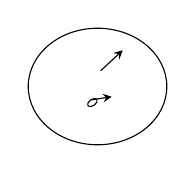
\begin{tikzpicture}[>=stealth,x=10mm,y=10mm]
  \draw (0,0) ellipse[x radius=.88,y radius=.74];
  \draw[rotate=35] (-.17,-.13) ellipse[x radius=.07,y radius=.04];
  \draw[->] (-.08,-.17) -- (.18,-.13);
  \draw[->] (.04,.20) -- (.32,.46);
\end{tikzpicture}}\endgroup}
\end{GelfandAdjacentEvidence}
\begin{GelfandAdjacentEvidence}{GELFAND-P001420}{8}


Or take the quotient by the maximal compact subgroup

\SourceFigure{GELFAND-P001420}{fundamental-domain}{%
\begingroup\color{black}\GelfandFitDiagram{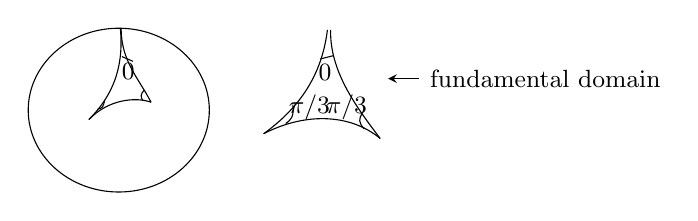
\begin{tikzpicture}[>=stealth,x=10mm,y=10mm,font=\small]
  \draw (0,0) ellipse[x radius=1.15,y radius=1.04];
  \draw (.02,1.04) .. controls (.06,.61) and (-.03,.23) .. (-.38,-.12);
  \draw (.03,1.04) .. controls (.03,.62) and (.25,.41) .. (.41,.10);
  \draw (-.38,-.12) .. controls (-.13,.14) and (.22,.17) .. (.41,.10);
  \draw (.04,.68)--(.18,.62)
    (-.27,.01) .. controls (-.20,.03) and (-.20,.04) .. (-.18,.12)
    (.31,.12) .. controls (.27,.16) and (.28,.21) .. (.32,.25);
  \node at (.12,.49) {\(0\)};
  \draw (2.65,1.02) .. controls (2.59,.54) and (2.38,.09) .. (1.84,-.30);
  \draw (2.69,1.02) .. controls (2.68,.50) and (3.00,.06) .. (3.32,-.36);
  \draw (1.84,-.30) .. controls (2.34,-.04) and (2.92,-.03) .. (3.32,-.36);
  \draw (2.56,.65)--(2.72,.69)
    (2.12,-.17) .. controls (2.23,-.10) and (2.22,-.01) .. (2.21,.07)
    (3.12,-.24) .. controls (3.04,-.16) and (3.05,-.11) .. (3.09,-.04);
  \node at (2.62,.48) {\(0\)};
  \node at (2.42,.03) {\(\pi/3\)};
  \node at (2.89,.03) {\(\pi/3\)};
  \draw[<-] (3.42,.40)--(3.81,.40);
  \node[anchor=west] at (3.83,.40) {\uwave{fundamental domain}};
\end{tikzpicture}}\endgroup}
\end{GelfandAdjacentEvidence}


\uwave{Answer.}
\[
\text{(2)}\quad
\operatorname{vol}\mathrm{SL}(n,\mathbb R)/\mathrm{SL}(n,\mathbb Z)
=\zeta(2)\zeta(3)\ldots\zeta(n)
\]

\(\mathbb A\) denotes the adeles.
\[
\begin{aligned}
\text{(3)}\quad\mathrm{SL}(n,\mathbb A)&\sim
\mathrm{SL}(n,\mathbb R)\times\mathrm{SL}(n,\mathbb Q_2)\times\ldots\\[-2pt]
 &\hspace{3.6em}\begin{gathered}\cup\\\mathrm{SL}(n,\mathbb Q)\end{gathered}
\end{aligned}
\]
\[
\text{(4)}\quad
\operatorname{vol}\mathrm{SL}(n,\mathbb A)/\mathrm{SL}(n,\mathbb Q)=1.
\]
\[
\begin{aligned}
\operatorname{vol}\mathrm{SL}(n,\mathbb A)/\mathrm{SL}(n,\mathbb Q)
 &\sim
 \operatorname{vol}\mathrm{SL}(n,\mathbb R)/\mathrm{SL}(n,\mathbb Z)\\
 &\qquad \prod\operatorname{vol}\mathrm{SL}(n,\mathbb Z_p).
\end{aligned}
\]
\[
\text{(5)}\quad
\operatorname{vol}\mathrm{SL}(n,\mathbb Z_p)
\sim\#\mathrm{SL}_n(\mathbb F_p)/p^{n^2-1}.
\]

\uline{Exercise}: compute \(\#\mathrm{SL}_n(\mathbb F_p)\).


\Needspace{7\baselineskip}
\begin{GelfandAdjacentEvidence}{GELFAND-P001421}{1}
\SourcePage{GELFAND-P001421}{unlabelled}

(6) Number of elements of \(\mathrm{GL}(n,\mathbb F_p)\)
\[
\begin{aligned}
 (p^n-1)(p^n-p)(p^n-p^2)\ldots
 &=
 p^{n^2}(1-p^{-n})(1-p^{-n+1})\ldots(1-p^{-1}).
\end{aligned}
\]

(7) For \(\mathrm{SL}(n,\mathbb F_p)\) divide by \(p-1\):
\[
 p^{n^2-1}(1-p^{-n})(1-p^{-n+1})\ldots(1-p^{-2}).
\]
This is a product of Euler factors.

(8) \uwave{Yu. I. Manin’s conjecture}: an analogue of formula (2) can be written for the moduli spaces of curves arising in string theory.

\uwave{I. M. G.}

\uwave{Mathematical question}: the volume of Teichmüller space has a \(p\)-adic analogue.

Or: what is adelic Teichmüller space

\uwave{An example of [moshchi?] of Witten’s work:}
\Unclear{GELFAND-P001421}{witten-heading-faint-word}{The faint word may read moshchi. The initial strokes are fragmentary and sily remains possible.}
\end{GelfandAdjacentEvidence}
\begin{GelfandAdjacentEvidence}{GELFAND-P001421}{2}


\uwave{Laumon} did work in number theory based on Witten’s ideas from Morse theory.

Idea: consider a function \(u\in\mathcal E'(\mathbb R)\),
\(\widetilde u(\xi)\in C^\infty\) and all the singularities will go into the asymptotics at infinity.

\uline{Advice from I. M. G.}: read Kharkevich’s book «Spectra,
[crossed out: illegible] [inserted above the line: Signals] and Noise»,
to understand the \uline{Fourier transform}.
\Incomplete{GELFAND-P001421}{book-title-cancelled}{The writing in the book title is crossed out. “Signals” is inserted above it.}
\end{GelfandAdjacentEvidence}
\begin{GelfandAdjacentEvidence}{GELFAND-P001421}{3}


On the work of \uwave{Laumon}.

\SourceFigure{GELFAND-P001421}{surface-figure}{%
\begingroup\color{black}\GelfandFitDiagram{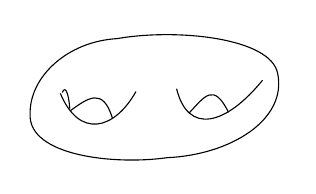
\begin{tikzpicture}[x=12mm,y=12mm]
  \draw (-1.3,-.18) .. controls (-1.31,.21) and (-.91,.59) .. (-.38,.62)
    .. controls (.25,.73) and (1.25,.63) .. (1.32,.25)
    .. controls (1.42,-.24) and (.82,-.61) .. (.15,-.64)
    .. controls (-.41,-.72) and (-1.32,-.62) .. cycle;
  \draw (-.98,.04) .. controls (-.78,-.44) and (-.41,-.35) .. (-.18,.06);
  \draw (-.87,-.14) .. controls (-.69,-.01) and (-.53,.11) .. (-.43,-.22);
  \draw (-.96,.05) .. controls (-.92,.14) and (-.89,.01) .. (-.88,-.12);
  \draw (.25,.09) .. controls (.37,-.40) and (.77,-.30) .. (1.16,.18);
  \draw (.38,-.17) .. controls (.55,.01) and (.64,.16) .. (.80,-.16);
\end{tikzpicture}}\endgroup
\par The short stroke at the left of the first loop follows the visible outline. Its purpose is unclear.}
\end{GelfandAdjacentEvidence}
\begin{GelfandAdjacentEvidence}{GELFAND-P001421}{4}


Consider a surface \(\mathcal F\)
\[
 H^i(X,\mathcal F),\qquad i=0,1,2.
\]
\EvidenceBlock{GELFAND-P001421}{surface-symbol}{After “surface” the manuscript writes \(\mathcal F\), and then \(H^i(X,\mathcal F)\).}{Manuscript notation.}
\end{GelfandAdjacentEvidence}
\begin{GelfandAdjacentEvidence}{GELFAND-P001421}{5}


\[
\text{(1)}\quad
\det H^\bullet(X,\mathcal F)=
\frac{\det H^0(X,\mathcal F)\det H^2(X,\mathcal F)}
{\det H^1(X,\mathcal F)\quad\text{[crossed out: }\det H^2(X,\mathcal F)\text{]}}
\]
\Unclear{GELFAND-P001421}{eq1-denominator}{The first superscript in the denominator is retraced and reads \(1\). The crossed-out factor tentatively reads \(\det H^2(X,\mathcal F)\).}
\end{GelfandAdjacentEvidence}
\begin{GelfandAdjacentEvidence}{GELFAND-P001421}{6}


([crossed out: finite?] vector spaces.
\(\det\) is the top exterior power)
\Unclear{GELFAND-P001421}{before-vector-spaces-cancelled}{The crossed-out word before “vector spaces” tentatively reads “finite.”}
\end{GelfandAdjacentEvidence}


Automorphisms?

Consider a triangulation. \(\det H^\bullet\) is identified with the product of the \(\det\)
of the terms of the complex (an Euler-type formula): canonically


\Needspace{7\baselineskip}
\begin{GelfandAdjacentEvidence}{GELFAND-P001422}{1}
\SourcePage{GELFAND-P001422}{64}

\[
\text{(2)}\quad\det(C^\bullet)=\det(H^\bullet(C))
\]
\(2-2g\) is the Euler characteristic.

On the other hand
\[
2g-2=\deg\underset{\substack{|\\\text{canonical class}}}{K}
\]

Let

\(D\) be a divisor.
\[
\text{(3)}\quad
\det\mathcal F_D=\bigotimes(\det\mathcal F_{x_i})^{\otimes a_i},
\qquad D=\sum a_i x_i
\]
[crossed out: \(D\longrightarrow D+K\)\textsuperscript{?}]
\Unclear{GELFAND-P001422}{cancelled-divisor-map}{The crossed-out writing shows \(D\), an arrow and a probable \(D+K\). Crossing strokes intersect the tail of the arrow.}
\end{GelfandAdjacentEvidence}
\begin{GelfandAdjacentEvidence}{GELFAND-P001422}{2}


\uwave{Deligne’s formula:}
\[
\text{(4)}\quad\det H^\bullet=\det\mathcal F_K
\]
\EvidenceBlock{GELFAND-P001422}{eq4-determinant-convention}{The right-hand side of (4) reads \(\det\mathcal F_K\) without the exponent \(-1\).}{Manuscript notation.}
\end{GelfandAdjacentEvidence}
\begin{GelfandAdjacentEvidence}{GELFAND-P001422}{3}

[At right: crossed out: illegible]
\Incomplete{GELFAND-P001422}{eq4-cancelled-sign}{The separate crossed-out mark to the right of the formula is illegible.}
\end{GelfandAdjacentEvidence}
\begin{GelfandAdjacentEvidence}{GELFAND-P001422}{4}


(fix the complex structure and the choice of a point in the canonical class)

For an arbitrary constructible sheaf one also computes \(\underline{\det}\) and there is an analogue of Deligne’s formula!

Here on \(\mathbb A^1\) functions with singularities arise

\uuline{Klyachko.}\qquad \uuline{Toric bundles.}

A toric variety is a variety \(X\) on which an algebraic torus \(T\),
acts, with an orbit isomorphic to \(T\).
\[
X=\bigcup_\sigma O_\sigma,\quad\text{is the decomposition into orbits}
\]

\(\mathcal E\) is a bundle over \(X\) with a toric structure
(and the action lifts! The diagram commutes)

\SourceFigure{GELFAND-P001422}{toric-bundle-square}{%
\begingroup\color{black}\GelfandFitDiagram{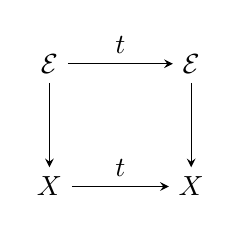
\begin{tikzpicture}[>=stealth,x=12mm,y=12mm]
  \node (source) at (0,1.3) {\(\mathcal E\)};
  \node (target) at (1.5,1.3) {\(\mathcal E\)};
  \node (baseleft) at (0,0) {\(X\)};
  \node (baseright) at (1.5,0) {\(X\)};
  \draw[->] (source) -- node[above]{\(t\)} (target);
  \draw[->] (baseleft) -- node[above]{\(t\)} (baseright);
  \draw[->] (source) -- (baseleft);
  \draw[->] (target) -- (baseright);
\end{tikzpicture}}\endgroup}
\end{GelfandAdjacentEvidence}


One can describe the moduli of [inserted above the line: «such»] bundles in the language of linear algebra.


\Needspace{7\baselineskip}
\begin{GelfandAdjacentEvidence}{GELFAND-P001423}{1}
\SourcePage{GELFAND-P001423}{unlabelled}

The structure of \(X\) is described by a fan \(\Sigma\) in the Lie algebra of the torus.

\SourceFigure{GELFAND-P001423}{fan-figure}{%
\begingroup\color{black}\GelfandFitDiagram{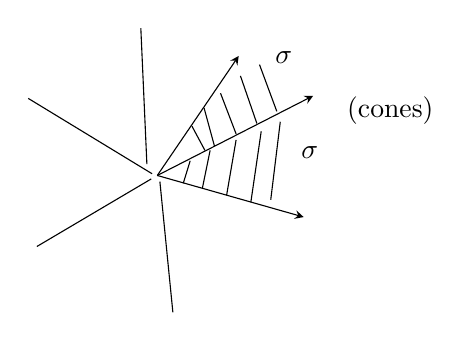
\begin{tikzpicture}[>=stealth,x=11mm,y=11mm]
  \draw (-1.49,.89)--(-.06,.02) (-1.39,-.82)--(-.07,-.04);
  \draw (-.19,1.70)--(-.12,.13) (.03,-.07)--(.18,-1.58);
  \draw[->] (0,0)--(.94,1.38);
  \draw[->] (0,0)--(1.80,.92);
  \draw[->] (0,0)--(1.69,-.48);
  \draw (.55,.29)--(.40,.57) (.66,.34)--(.54,.78)
    (.91,.48)--(.73,.95) (1.15,.60)--(.96,1.15) (1.38,.74)--(1.18,1.28);
  \draw (.30,-.09)--(.38,.17) (.52,-.15)--(.61,.29)
    (.80,-.23)--(.91,.41) (1.08,-.31)--(1.20,.51) (1.31,-.28)--(1.42,.62);
  \node at (1.46,1.36) {\(\sigma\)};
  \node at (1.76,.26) {\(\sigma\)};
  \node[anchor=west] at (2.08,.75) {(cones)};
\end{tikzpicture}}\endgroup}
\end{GelfandAdjacentEvidence}
\begin{GelfandAdjacentEvidence}{GELFAND-P001423}{2}


\(|\Sigma|\) is the set of \(1\)-dimensional cones in the fan \(\Sigma\).

\uline{Theorem.}
(category of toric bundles) \(\Longleftrightarrow\)
(category of vector spaces [crossed-out sign: illegible] \(E\)
with a collection of [inserted above the line: «decreasing \(\mathbb Z\)-indexed»]
filtrations \(E^\alpha(i)\), \(\alpha\in|\Sigma|\), satisfying the condition
\Incomplete{GELFAND-P001423}{theorem-cancelled-sign}{The crossed-out mark before \(E\) is illegible.}
\end{GelfandAdjacentEvidence}
\begin{GelfandAdjacentEvidence}{GELFAND-P001423}{3}


A) The filtrations \(E^\alpha\), \(\alpha\in\sigma\in\Sigma\), are distributive.

\uline{Problems.}
1) Describe the geometry of the bundle (cohomology, characteristic classes, and so on) in terms of the filtrations

2) classification — ?

Let \(\Sigma\) be a simplicial complex. Assign a filtration to a vertex

A representation of it is a collection of filtrations in a vector space [inserted above the line: «\(E\):»] \(E^\alpha(i)\),
\(\alpha\in\) [crossed-out sign: illegible] \(\Sigma\),
\Incomplete{GELFAND-P001423}{representation-cancelled-sign}{The mark between \(\in\) and \(\Sigma\) is crossed out and illegible.}
\end{GelfandAdjacentEvidence}
\begin{GelfandAdjacentEvidence}{GELFAND-P001423}{4}

\[
E\ldots\supset E^\alpha(i)\supset E^\alpha(i+1)\supset\ldots 0
\]
\[
\alpha\in(\text{vertices of the complex})=\Sigma.
\]

The spaces \(E^\alpha(i)\), \(\alpha\in\underset{\substack{|\\\text{simplex}}}{\sigma}\),
are distributive for fixed \(\sigma\) (for all \(i\))

[Outlined insertion: (i.e., they generate a distributive lattice)]

For example, if

\(\alpha_1,\alpha_2,\alpha_3\) are the vertices of a triangle, then

\(E^{\alpha_1}\quad E^{\alpha_2}\quad E^{\alpha_3}\) are distributive, i.e.,
\[
(E^{\alpha_1}+E^{\alpha_2})\cap E^{\alpha_3}
=E^{\alpha_1}\cap E^{\alpha_3}+E^{\alpha_2}\cap E^{\alpha_3}
\]

\uwave{Classify}: a good problem

For a triangle, the solution is trivial

For the surface of a tetrahedron \(\Sigma=\partial\Delta\), \(\Delta\) is a simplex, and the answer is as follows. In
[crossed out: \(\mathbb R^3\)-pr-ve?] \(E\), \(\dim E=3\), consider \(4\) \(2\)-dimensional subspaces in general position.
\Unclear{GELFAND-P001423}{tetrahedron-cancelled-space}{The crossed-out writing may read \(\mathbb R^3\)-pr-ve. Crossing strokes intersect the abbreviation.}
\end{GelfandAdjacentEvidence}
\begin{GelfandAdjacentEvidence}{GELFAND-P001423}{5}

\[
\mathcal E=(E;\ E^\alpha,E^\beta,E^\gamma,E^\delta)
\]
\Unclear{GELFAND-P001423}{tetrahedron-last-index}{The last superscript reads \(\delta\), as in the next expression. The lower loop is retraced.}
\end{GelfandAdjacentEvidence}



\Needspace{7\baselineskip}
\begin{GelfandAdjacentEvidence}{GELFAND-P001424}{1}
\SourcePage{GELFAND-P001424}{65}
we still need to take [above the line: ikh?] exterior powers
\[
\Lambda^i\mathcal E=
(\Lambda^i E,\Lambda^i E^\alpha,\Lambda^i E^\beta,
 \Lambda^i E^\gamma,\Lambda^i E^\delta)
\]
\Unclear{GELFAND-P001424}{exterior-insertion}{The insertion may read ikh. Its strokes overlap the insertion mark.}
\end{GelfandAdjacentEvidence}
\begin{GelfandAdjacentEvidence}{GELFAND-P001424}{2}

A general representation decomposes into a direct sum of \(1\)-dimensional ones and ones of this kind.

\uwave{I. M. G.}
The right problem: isolate in \(\forall\) problem the solvable pieces. (Gelfand–Ponomarev philosophy)

V. [crossed-out initial: illegible] \uwave{Kac} describes all this in the language of graphs and
Kac–Moody algebras:
vertex dimensions \(=\) root coordinates, etc.
\Unclear{GELFAND-P001424}{kac-initial}{The crossed-out initial between “V.” and “Kac” is illegible.}
\end{GelfandAdjacentEvidence}
\begin{GelfandAdjacentEvidence}{GELFAND-P001424}{3}


The number of parameters is determined.

Lect. Notes, \uwave{996}; an earlier work — \uwave{Inventiones}.
(conference talk)

[Crossed out: Seminar? \ldots]
\Unclear{GELFAND-P001424}{cancelled-seminar-line}{The first word of the crossed-out line tentatively reads “Seminar.”}
\end{GelfandAdjacentEvidence}
\begin{GelfandAdjacentEvidence}{GELFAND-P001424}{4}

\Incomplete{GELFAND-P001424}{cancelled-seminar-content}{The rest of the crossed-out line is illegible.}
\end{GelfandAdjacentEvidence}


\uwave{Next time:}\quad \uwave{8 February}.



\clearpage\pdfbookmark[0]{Chapter 32}{gelfand-archive-chapter-32}
\section*{Chapter 32}


\Needspace{7\baselineskip}
\begin{GelfandAdjacentEvidence}{GELFAND-P001425}{1}
\SourcePage{GELFAND-P001425}{1}
\uline{8/II--88 } \quad \uline{Gelfand Seminar.}

I. M. G. \uline{Problems.} 1. Evaluate
\begin{equation*}
\tag{1}\det\left\Vert\frac{1}{x_i-y_k}\right\Vert_{i,k=1}^{n}.
\end{equation*}
2. Prove that the Legendre polynomial
\[
\bigl((x^2-1)^n\bigr)^{(n)}
\]
has only real zeros.

3. Can a function that is the limit of continuous functions at every point of a closed interval

a) have discontinuities?

b) have an everywhere dense set of points of discontinuity?

c) be discontinuous everywhere (i.e., at every point)?

4. \textbf{Map conformally onto the disc}

a) (disc with a radius removed!)
\SourceFigure{GELFAND-P001425}{slit-disc}{%
\begingroup\color{black}\GelfandFitDiagram{\begin{tikzpicture}[x=11mm,y=11mm]
  \draw (0,0) circle (.58);
  \draw (0,0)--(.58,0);
  \fill (0,0) circle (.024);
\end{tikzpicture}}\endgroup}
\end{GelfandAdjacentEvidence}
\begin{GelfandAdjacentEvidence}{GELFAND-P001425}{2}


b)
\SourceFigure{GELFAND-P001425}{joined-discs}{%
\begingroup\color{black}\GelfandFitDiagram{\begin{tikzpicture}[>=stealth,x=10mm,y=10mm]
  \draw (.68,.10) arc[start angle=8,end angle=352,radius=.687]
    --(4.82,-.10) arc[start angle=188,end angle=532,radius=.687] --cycle;
  \draw[->] (0,0)--(.19,.65);
  \node[left] at (.10,.35) {\(1\)};
  \draw[->] (5.50,0)--(6.12,.26);
  \node[above] at (5.66,.17) {\(1\)};
  \draw[->] (1.8,.58)--(1.8,.10);
  \draw[->] (1.8,-.62)--(1.8,-.10);
  \node[above right] at (1.8,.26) {\(10^{-6}\)};
  \fill (2.62,0) circle (.022);
  \node[right] at (2.64,-.30) {\(A\)};
  \draw[->] (2.61,-.09)--(2.47,-1.43);
  \draw (2.47,-2.27) circle (.58);
  \draw[->] (2.47,-2.27)--(2.47,-1.69);
  \node[left] at (2.47,-2.04) {\(1\)};
  \node[right] at (2.47,-2.27) {\(0\)};
  \node[anchor=west] at (3.37,-1.36) {\(A\mapsto\) centre of the disc};
\end{tikzpicture}}\endgroup}
\end{GelfandAdjacentEvidence}
\begin{GelfandAdjacentEvidence}{GELFAND-P001425}{3}


\uuline{\textbf{A. Beilinson.}}\qquad \uline{What does one need to know about string theory?}

\uline{Conformal field theory.} \quad (2-dimensional)

Operator expansion.

Connection with representations of natural infinite-dimensional Lie algebras.

\(W\)-algebras, parafermions.

[Crossed out: Ve\ldots{} / Ver\ldots{}?] Algebra of \uwave{vertex} operators.
\Unclear{GELFAND-P001425}{vertex-cancellation}{“Ve\ldots{}” is discernible under the crossing-out. The descending stroke may belong to an \(r\).}
\end{GelfandAdjacentEvidence}
\begin{GelfandAdjacentEvidence}{GELFAND-P001425}{4}

\Unclear{GELFAND-P001425}{vertex-retracing}{The word reads “vertex.” The earlier strokes at its beginning cannot be distinguished.}
\end{GelfandAdjacentEvidence}


Various reductions of representations of \(\widehat{SL}_2\) to the Virasoro algebra.

Connection with moduli spaces of algebro-geometric structures.

Explicit formulas for partition functions and [Crossed out: correlation functions; inserted above the line: correlators].

Branching property of characters.


\Needspace{7\baselineskip}
\begin{GelfandAdjacentEvidence}{GELFAND-P001426}{1}
\SourcePage{GELFAND-P001426}{unlabelled}
\uuline{D. Alekseevsky.}\qquad \uuline{\(G\)-structures}

\uwave{Scalar field quantity}.

[crossed out: Field] — a function of the point \(x\in\mathbb R^3\) with vector values

(e.g., with values in \(\mathbb R\))

\uwave{Field quantity}: depends on the coordinate system

\uuline{\(G\)-structure}.

\uuline{Def. 1}\quad \(G\subset GL(V)\), \(V=\mathbb R^n\).

[Under \(G\): linear group.]

\(G\)-structure [above the line: on \(M^n\)] — a principal subbundle of the manifold of all
[crossed out: ko?]frames.

[On the right, under «frames»: (coframes) — is better to say.]
\Unclear{GELFAND-P001426}{frame-prefix}{The crossed-out letters before “frames” tentatively read “ko.” The separate note below reads “(coframes).”}
\end{GelfandAdjacentEvidence}
\begin{GelfandAdjacentEvidence}{GELFAND-P001426}{2}


\SourceFigure{GELFAND-P001426}{frame-bundle}{%
\begingroup\color{black}\GelfandFitDiagram{\begin{tikzpicture}[>=stealth,x=12mm,y=9mm]
  \node (frames) at (0,0) {\(M^{(1)}\)};
  \node (base) at (2.6,0) {\(M\)};
  \draw[->] (frames) -- node[above] {\(GL(V)\)} (base);
  \node[align=left,anchor=north west] at (-.65,-.26)
    {frame bundle \\ (principal bundle)};
\end{tikzpicture}}\endgroup}
\end{GelfandAdjacentEvidence}
\begin{GelfandAdjacentEvidence}{GELFAND-P001426}{3}


\SourceFigure{GELFAND-P001426}{frame-diagram}{%
\begingroup\color{black}\GelfandFitDiagram{\begin{tikzpicture}[>=stealth,x=11mm,y=9mm]
  \node (frames) at (0,0) {\(M^{(1)}\)};
  \node (base) at (2.7,-.10) {\(M\)};
  \node (reduction) at (0,-1.8) {\(P\)};
  \draw[->] (frames) -- node[above] {\(GL(V)\)} (base);
  \node at (0,-.90) {\(\cup\)};
  \draw[->] (reduction) -- node[below right] {\(G\)} (base);
\end{tikzpicture}}\endgroup}
\end{GelfandAdjacentEvidence}
\begin{GelfandAdjacentEvidence}{GELFAND-P001426}{4}


\(G\) must act on \(P\) transitively.
\EvidenceBlock{GELFAND-P001426}{transitivity}{The manuscript says “on \(P\) transitively.”}{Manuscript notation.}
\end{GelfandAdjacentEvidence}
\begin{GelfandAdjacentEvidence}{GELFAND-P001426}{5}


Then this is precisely a \(G\)-structure.

\uline{Examples}: 1) a Riemannian metric is an \(O(V)\)-structure

2) Let \(S\) be a tensor field. When does it define a \(G\)-structure?

If they are all of the same canonical form

(at \(\forall\) point \(\exists\) a coframe
[crossed out: \(\theta\) / \(\varphi\)?], bringing \(S\) to a fixed form)
\Unclear{GELFAND-P001426}{tensor-cancellation}{The crossed-out sign after “coframe” resembles \(\theta\) or \(\varphi\).}
\end{GelfandAdjacentEvidence}


Then if \(G\) — the group of automorphisms of the canonical form, then \(S\) defines a \(G\)-structure.

3) An affinor defines a \(G\)-structure, if at \(\forall\) point the Jordan form is the same

4) Almost complex structure \(J\): \(G=GL\bigl(\frac{n}{2},\mathbb C\bigr)\)

5) Almost symplectic structure: \(2\)-form \(\sigma\) of maximal rank,

(\uwave{symplectic structure}: \(d\sigma=0\))

\uline{Def. 2}\quad \(G\)-structure — a principal \(G\)-bundle
\(\pi\colon P\overset{G}{\longrightarrow}M\)

\(G\subset GL(V)\)

equipped with a vector-valued \(1\)-form \(\theta\colon TP\to V\),

satisfying the following conditions:


\Needspace{7\baselineskip}
\begin{GelfandAdjacentEvidence}{GELFAND-P001427}{1}
\SourcePage{GELFAND-P001427}{2}
a) \(G\)-equivariance

b) \(\operatorname{Ker}\theta=T^vP\) (vertical space), i.e.,
\(\theta\) is strictly horizontal.

\uwave{Equivalence of definitions 1 and 2.}

\(p\in P\), \(x=\pi p\);
\[
\theta_p\colon
\underset{\substack{\downarrow\\ (T_pM/T_p^vM)}}{\underbrace{T_xM}}
\overset{\simeq}{\longrightarrow}V.
\]
[On the right:] this is precisely the coframe with which we identify the point \(p\).
\EvidenceBlock{GELFAND-P001427}{quotient-notation}{Below \(T_xM\) is \(T_pM/T_p^vM\), with \(M\) written in both terms.}{Manuscript notation.}
\end{GelfandAdjacentEvidence}
\begin{GelfandAdjacentEvidence}{GELFAND-P001427}{2}


[Crossed out: \(\theta_p\) on vertik\ldots{}? \(\,0\).]
\Unclear{GELFAND-P001427}{zero-cancellation}{The crossed-out line shows \(\theta_p\), “on,” and \(0\). The intervening word tentatively reads “vertik\ldots{}”.}
\end{GelfandAdjacentEvidence}
\begin{GelfandAdjacentEvidence}{GELFAND-P001427}{3}


Coframe \(\simeq\) an isomorphism
\(\theta_p\colon T_xM\overset{\simeq}{\longrightarrow}V\)

\(\theta\) is called \uwave{the solder form}

\begin{center}
\(\rule{1.2cm}{.3pt}\ \cdot\ \rule{1.2cm}{.3pt}\)
\end{center}

Suppose there is a \(G\)-structure
\[
(\pi\colon P\overset{G}{\longrightarrow}M;\theta)
\]
Consider the bundle of 1-jets of the bundle \(\pi\)
\[
\pi'\colon P'\to P
\]
\(x\to p_x\) is a section
\[
p'\colon T_xM\to T_{p_x}P
\]

\uline{Def.} A 1-jet is a map \(p'\) — inverse to the projection, \(p'=j_x^1(p)\)

\SourceFigure{GELFAND-P001427}{jet-diagram}{%
\begingroup\color{black}\GelfandFitDiagram{\begin{tikzpicture}[>=stealth,x=10mm,y=8mm]
  \node (label) at (0,0) {\(p'=j_x^1(p)\colon\)};
  \node (base) at (2.16,0) {\(T_xM\)};
  \node (total) at (4.43,0) {\(T_{p_x}P\)};
  \draw[->] (base) -- (total);
  \draw[->] (total.south west) to[bend left=32] (base.south east);
\end{tikzpicture}}\endgroup}
\end{GelfandAdjacentEvidence}
\begin{GelfandAdjacentEvidence}{GELFAND-P001427}{4}

i.e., \(\pi_*\circ p'=\mathrm{id}\)

\uline{Def.} A horizontal subspace \(H\subset T_pP\),
[Crossed out: illegible] — is a subspace such that
\Incomplete{GELFAND-P001427}{horizontal-cancellation}{The crossed-out mark after \(T_pP\) is illegible.}
\end{GelfandAdjacentEvidence}
\begin{GelfandAdjacentEvidence}{GELFAND-P001427}{5}

\[
T_pP=T_p^v\oplus H
\]

\uline{Second definition of a 1-jet}

\[
\underbrace{\text{Elements of }P'}_{\text{(\(=\) 1-jets)}}
=\text{\uwave{horizontal subspaces}}
\]
\[
p'\in P'\quad\Longleftrightarrow\quad H(p')\text{ — a horizontal subspace}
\]
\uwave{Relation}:
\[
p'\colon T_xM\to H(p')\subset T_pP
\]
\uline{Def.} [Crossed out: \(P'\)?]
\(\pi'\) is called \uwave{the bundle of connections}.
\Unclear{GELFAND-P001427}{connection-cancellation}{The crossed-out mark before \(\pi'\) may read \(P'\).}
\end{GelfandAdjacentEvidence}



\Needspace{7\baselineskip}
\begin{GelfandAdjacentEvidence}{GELFAND-P001428}{1}
\SourcePage{GELFAND-P001428}{unlabelled}
\uwave{Space of connections}:\quad \(\Gamma(\pi')^G\)

(i.e., a connection is a \(G\)-equivariant section of the bundle \(\pi'\colon P'\to P\))

\uwave{Connection}:
\[
\begin{aligned}
h\colon P&\to P'\\
p&\mapsto H(p)
\end{aligned}
\]
(\(G\)-invariant field of horizontal subspaces)

This gives parallel transport (restrict to a curve)

\uline{Torsion function}\qquad (analogue of the structure constants of a Lie group)

There is a vertical parallelism:
\[
\begin{aligned}
i_p\colon\mathfrak g&\underset{\simeq}{\longrightarrow}T_p^vP\\
X&\mapsto X_p:=\left.\frac{d}{dt}(\exp tX)p\right|_{t=0}
\end{aligned}
\]
\EvidenceBlock{GELFAND-P001428}{vertical-generator}{The \(p\) following \((\exp tX)\) is retraced. It is written to the right of the exponential.}{Manuscript notation.}
\end{GelfandAdjacentEvidence}
\begin{GelfandAdjacentEvidence}{GELFAND-P001428}{2}


\SourceFigure{GELFAND-P001428}{decomposition-diagram}{%
\begingroup\color{black}\GelfandFitDiagram{\begin{tikzpicture}[>=stealth,x=10mm,y=8mm]
  \node at (0,0) {\(p'\in P'\Longrightarrow T_pP=\)};
  \node (vertical) at (3.10,0) {\(T_p^v\)};
  \node at (4.43,0) {\(\oplus H(p')\)};
  \node at (-.62,-.89) {\(\pi'(p')=p\)};
  \node (algebra) at (3.10,-2.12) {\(\mathfrak g\)};
  \draw[->] (vertical) -- node[right] {\(i_p^{-1}\)} (algebra);
\end{tikzpicture}}\endgroup}
\end{GelfandAdjacentEvidence}
\begin{GelfandAdjacentEvidence}{GELFAND-P001428}{3}

[After the \(=\) sign, crossed out: illegible]
\Incomplete{GELFAND-P001428}{decomposition-cancellation}{The mark between \(=\) and \(T_p^v\) is crossed out and illegible.}
\end{GelfandAdjacentEvidence}
\begin{GelfandAdjacentEvidence}{GELFAND-P001428}{4}


Take the form \(\theta_p\colon T_pP\to V\)
\Unclear{GELFAND-P001428}{theta-domain}{Both subscripts \(p\) and the letter \(P\) are retraced or overwritten.}
\end{GelfandAdjacentEvidence}
\begin{GelfandAdjacentEvidence}{GELFAND-P001428}{5}


and set
\[
\theta_{H(p')}=\theta|_{H(p')}\colon H(p')\overset{\simeq}{\longrightarrow}V
\]
\uline{Def.}\quad \uwave{The torsion function} — is the map
\[
t\colon P'\longrightarrow\operatorname{Hom}(V\wedge V,V)
\]
(tensors of type \(1,2\))
\[
p'\mapsto t_{p'},\qquad
t_{p'}(\xi,\eta)=d\theta\bigl(\theta_{H(p')}^{-1}\xi,\theta_{H(p')}^{-1}\eta\bigr)
\]
\EvidenceBlock{GELFAND-P001428}{torsion-last-argument}{The last symbol has a differently shaped initial stroke and reads as \(\eta\).}{Manuscript notation.}
\end{GelfandAdjacentEvidence}


\uwave{Properties of the torsion function}.

1) \(G\)-equivariance and \(G'=\operatorname{Hom}(V,\mathfrak g)\)-equivariance


\Needspace{7\baselineskip}
\begin{GelfandAdjacentEvidence}{GELFAND-P001429}{1}
\SourcePage{GELFAND-P001429}{3}
\uline{15/II--88 }\qquad \uuline{Gelfand Seminar}
(from the notes of A. K. Zvonkin)

In I. M. G.'s lectures on quasilinear equations
(\href{https://www.mathnet.ru/eng/rm7290}{UMN, 1959, vol. 14, no. 2})
three pages present \uline{all of thermodynamics}.

\uwave{A concrete problem in geometry}: what is the angle between two \(2\)-dimensional subspaces in \(4\)-dimensional space?

The angle is an invariant of relative motion (for lines).

There are \(2\) versions, for oriented lines and for unoriented lines.

For planes, how many such invariants are there and what are they?

\uuline{Question}: find all the invariants of two subspaces of a Hilbert space.

[Crossed out: Zam\ldots{}?]
\Unclear{GELFAND-P001429}{speaker-cancellation}{The crossed-out writing above the name tentatively begins “Zam…”.}
\end{GelfandAdjacentEvidence}
\begin{GelfandAdjacentEvidence}{GELFAND-P001429}{2}


\uuline{Zamolodchikov, Sasha.}\qquad
\uline{Conformal (2-dimensional) field theory.}

\begin{equation*}
\tag{1}
\langle A_1(x_1)A_2(x_2)\ldots A_N(x_N)\rangle,\qquad x_i\in\mathbb R^2,
\end{equation*}
— «correlation functions»

\(\mathcal A\ni A\) — fields (in general infinite-dimensional)

(1) — \(N\)-linear function on the space of fields \(\mathcal A\)
(also a function of \((x_1,\ldots,x_N)\))

Let us specify the meaning of the average in (1):
\begin{equation*}
\tag{2}
(1)=Z^{-1}\int\mathcal D\varphi\, e^{-S[\varphi]}A_1(x_1)\ldots A_N(x_N),
\end{equation*}
where \(\varphi=\varphi(x)\),
\begin{equation*}
\tag{3}
S=\int\sigma\bigl(\varphi(x),\partial\varphi(x)\bigr)\,dx,
\end{equation*}
\begin{equation*}
\tag{4}
Z=\int\mathcal D\varphi\,e^{-S[\varphi]}.
\end{equation*}
\Unclear{GELFAND-P001429}{equation-number}{The number (4) is written over a digit resembling 3.}
\end{GelfandAdjacentEvidence}
\begin{GelfandAdjacentEvidence}{GELFAND-P001429}{3}


\uwave{Properties of the correlation functions}.

1) «Algebra of fields»

Let the fields form an associative algebra; [Crossed out: illegible]
with [inserted above the line: (with a continuum)] generators [Russian ending uncertain] \(A_i(x)\).
\Incomplete{GELFAND-P001429}{algebra-cancellation}{The writing immediately after the semicolon is crossed out and illegible.}
\end{GelfandAdjacentEvidence}
\begin{GelfandAdjacentEvidence}{GELFAND-P001429}{4}

\Unclear{GELFAND-P001429}{algebra-ending}{The overwritten Russian ending allows the readings “obrazuiushchimi” and “obrazuiushchikh” for “generators.” The strokes in \(A_i(x)\) are also retraced.}
\end{GelfandAdjacentEvidence}


Let \(\{A_i\}\) — be a basis in \(\mathcal A\). Then
\[
A_i(x)A_j(y)=\sum_k
\underset{\substack{\uparrow\\ \text{numerical functions of }x,y}}
  {\underbrace{c_{ij}^k(x,y)}}\,A_k(y)
\]

Set
\[
\langle A_k(x)\rangle=a_k(x)
\]


\Needspace{7\baselineskip}
\begin{GelfandAdjacentEvidence}{GELFAND-P001430}{1}
\SourcePage{GELFAND-P001430}{unlabelled}
(Knowing the functions \(c_{ij}^k\) and \(a_k\) is sufficient to compute the correlation functions:
we replace the pair \(A_1A_2\) by \(\sum c^kA_k\) and so on)

2) «\uwave{Invariance}»

Consider a field \(T\) of the form
\[
T^{\mu\nu},\quad\mu,\nu=1,2;\quad T^{\mu\nu}\in\mathcal A.
\]
Incidentally
\begin{equation*}
\tag{5}
\frac{\partial}{\partial x^\mu}A_i(x)A_j(y)
=\sum\frac{\partial}{\partial x^\mu}c_{ij}^k(x,y)A_k.
\end{equation*}
\begin{equation*}
\tag{6}
\frac{\partial T^{\mu\nu}}{\partial x^\mu}=0
\end{equation*}

Consider [crossed out: operator?] the integral
\begin{equation*}
\tag{7}
\oint T^{\mu\nu}(x)A(y)\,\varepsilon_{\mu\lambda}\,dx^\lambda
\end{equation*}
\Unclear{GELFAND-P001430}{integral-cancellation}{The crossed-out word tentatively reads “operator.”}
\end{GelfandAdjacentEvidence}
\begin{GelfandAdjacentEvidence}{GELFAND-P001430}{2}

\Unclear{GELFAND-P001430}{epsilon-first-index}{The second index of \(\varepsilon\) is overwritten. It reads \(\lambda\), possibly over \(\nu\).}
\end{GelfandAdjacentEvidence}
\begin{GelfandAdjacentEvidence}{GELFAND-P001430}{3}

[To the right of the integral]
\SourceFigure{GELFAND-P001430}{contour-diagram}{%
\begingroup\color{black}\GelfandFitDiagram{\begin{tikzpicture}[>=stealth]
  \draw (0,0) circle (.56);
  \draw[->] (160:.56) arc[start angle=160,end angle=119,radius=.56];
  \fill (-.05,-.015) circle (.021);
  \node at (.14,-.10) {\(y\)};
\end{tikzpicture}}\endgroup}
\end{GelfandAdjacentEvidence}
\begin{GelfandAdjacentEvidence}{GELFAND-P001430}{4}


[Callout to \(\varepsilon\) in (7):]
\[
\varepsilon_{\mu\lambda}=-\varepsilon_{\lambda\mu},\qquad\varepsilon_{12}=1
\]
It defines a linear operator in \(\mathcal A\).

\uline{Required}: \(\exists\) a field \(T\) such that this operator equals \(\dfrac{\partial}{\partial y}\).

\(T^{\mu\nu}:=\) «energy–momentum tensor»
\[
\oint T^{\mu\nu}(x)A_i(y)\,\varepsilon_{\mu\nu}\,dx^\lambda
=\frac{\partial}{\partial y^\nu}A_i(y)
\]
\EvidenceBlock{GELFAND-P001430}{epsilon-repeat}{In the repeated formula the second index of \(\varepsilon\) reads \(\nu\), alongside \(dx^\lambda\).}{Manuscript notation.}
\end{GelfandAdjacentEvidence}


\(1')\)\quad \(c_{ij}^k(x,y)=c_{ij}^k(x-y)\) — functions of one variable in \(\mathbb R^2\).

3) «\uwave{Positivity condition}»

\(A\mapsto A^+\in\mathcal A\) — involution
\begin{equation*}
\tag{8}
A_i^+(x)A_j^+(y)=\sum\overline c_{ij}^k(\widetilde x-\widetilde y)A_k^+(y)
\end{equation*}
\[
x=(x^1,x^2)\quad\Rightarrow\quad\widetilde x=(-x^1,x^2)
\]
\uline{Requirement}: the matrix \(\langle A_i^+(\widetilde x)A_j(x)\rangle\)
is positive definite for all \(x\).

\uline{The problem} is to construct substantive examples of all this.


\Needspace{7\baselineskip}
\begin{GelfandAdjacentEvidence}{GELFAND-P001431}{1}
\SourcePage{GELFAND-P001431}{4}
Let us introduce in \(\mathbb R^2\) complex coordinates
\[
z=x^1+ix^2\qquad ds^2=dz\,d\bar z
\]
\begin{equation*}
\tag{9}
T^{\nu\mu}=T^{\mu\nu}
\end{equation*}
\begin{equation*}
\tag{10}
\left.\begin{aligned}
T&=T^{zz},\quad \bar T=T^{\bar z\bar z}\\
\Theta&=T^{z\bar z}=0
\end{aligned}\right\}\quad
\begin{gathered}
\text{under these additional conditions}\\
\text{the theory is called}\\
\text{«conformal field theory»}
\end{gathered}
\end{equation*}
[Arrow from below to \(\Theta=0\):] Important special case: massless theory
\EvidenceBlock{GELFAND-P001431}{tensor-components}{In (10) both upper indices in the definition of \(\bar T\) have a bar: \(\bar T=T^{\bar z\bar z}\).}{Manuscript notation.}
\end{GelfandAdjacentEvidence}
\begin{GelfandAdjacentEvidence}{GELFAND-P001431}{2}


\uline{Check question}: write \(T^{zz}\), \(T^{z\bar z}\), \(T^{\bar z\bar z}\)
in terms of \(T^{\mu\nu}\)

(this is a linear algebra problem)
\begin{equation*}
\tag{11}
\frac{\partial T}{\partial\bar z}=0,\quad
\frac{\partial\bar T}{\partial z}=0
\qquad\text{— Cauchy–Riemann equations}
\end{equation*}
\[
\Updownarrow
\]
\(T\) — an analytic function of \(z\), \(T=T(z)\), \(\bar T=\bar T(\bar z)\).
\begin{equation*}
\tag{12}
T(z)A_i(z_1,\bar z_1)=\sum f_{ij}(z-z_1)A_j(z_1,\bar z_1)
\end{equation*}

\uline{In electrodynamics}.

\(\psi\) — electron

\(A\) — photon
\[
\{A_i\}=\{\psi,\psi^2,\psi\partial\psi,\ldots,A,A^2,A\psi,\ldots\}
\]
\(\psi^4\) still exists, but \(\psi^5=\psi^6=0\) (since the spinor has only 4 components)

for \(A\) all powers exist

But, in general, \(A^2\) does not exist.

Do not take the fields at the same point. Take them at different points.
\begin{equation*}
\tag{13}
\oint\frac{dz}{2\pi i}\,z^{n+1}T(z)A_i(z_1,\bar z_1)
=L_nA_i(z_1,\bar z_1)
\end{equation*}
[To the right of (13):]
\SourceFigure{GELFAND-P001431}{mode-contour}{%
\begingroup\color{black}\GelfandFitDiagram{\begin{tikzpicture}
  \draw (0,0) circle (.53);
  \fill (-.08,.035) circle (.021);
  \node at (.14,-.04) {\(z_1\)};
  \node at (0,-.84) {\(n=0,\pm1,\pm2,\ldots\)};
\end{tikzpicture}}\endgroup}
\end{GelfandAdjacentEvidence}

\[
L_{-1}=\frac{\partial}{\partial z_1}
\]
\begin{equation*}
\tag{14}
\bar T(\bar z)\to\bar L_n;\quad
\bar L_{-1}=\frac{\partial}{\partial\bar z_1}
\end{equation*}
\(T(z_1)T(z_2)\) — is a function of \(z_1\), analytic everywhere except at \(z_2\);
let us expand it in a Laurent series.


\Needspace{7\baselineskip}
\begin{GelfandAdjacentEvidence}{GELFAND-P001432}{1}
\SourcePage{GELFAND-P001432}{unlabelled}
\begin{equation*}
\tag{15}
T(z_1)T(z_2)=\sum_{m=-\infty}^{\infty}(z_1-z_2)^mT_m(z_2),\qquad
T_m\in\mathcal A
\end{equation*}
Let us make an assumption:
\begin{equation*}
\tag{16}
(15)=(z_1-z_2)^{-4}T_{-4}+(z-z_2)^{-3}T_{-3}+\ldots
\end{equation*}
(i.e., the series terminates at its lower end at term \(-4\))
\EvidenceBlock{GELFAND-P001432}{laurent-factor}{The second power in (16) is written \((z-z_2)^{-3}\), without a subscript on its first \(z\).}{Manuscript notation.}
\end{GelfandAdjacentEvidence}
\begin{GelfandAdjacentEvidence}{GELFAND-P001432}{2}

\begin{equation*}
\tag{17}
T_{-1}=\frac{dT}{dz_2}(z_2)
\end{equation*}
\begin{equation*}
\tag{18}
\begin{aligned}
T_{-2}=2T(z_2)&\quad\leftarrow\quad\text{follows from the fact that}\\
&\hphantom{\quad\leftarrow\quad}\text{\(T\) is a rank-2 tensor}
\end{aligned}
\end{equation*}
The most important thing is to determine the most singular terms \(T_{-3}\) and \(T_{-4}\).

It follows from the positivity condition that
\begin{equation*}
\tag{19}
T_{-4}\sim\text{identity operator}:\quad T_{-4}=\frac c2,\qquad T_{-3}=0
\end{equation*}
\begin{equation*}
\tag{20}
T(z)T(z')=\frac{c}{2(z-z')^4}+\frac{2T(z')}{(z-z')^2}
+\frac{1}{z-z'}T'(z')+\ldots
\end{equation*}
[Arrow to the ellipsis in (20):] the further terms are of no interest

From this expansion we obtain
\begin{equation*}
\tag{21}
\boxed{[L_n,L_m]=(n-m)L_{n+m}+\frac{c}{12}(n^3-n)\delta_{n+m,0}}
\end{equation*}
These are the relations of the \uwave{Virasoro algebra} (central extension of the algebra of vector fields on the circle)

(In ordinary quantum mechanics, the Lie algebra of the group of translations on the line: \(\frac{d}{dx}\) — small translation — momentum)

In general the energy–momentum tensor comes from coordinate transformations

In this sense Sophus Lie invented quantum mechanics. He was the first to replace coordinate transformations with infinitesimal transformations.

(The group for the Virasoro algebra is the group of diffeomorphisms of the circle.)

\end{GelfandAdjacentEvidence}
\begin{GelfandAdjacentEvidence}{GELFAND-P001432}{3}
Lengths smaller than \(10^{-31}\) cm have no meaning. This statement is already independent [crossed out: от / не?]
of any theory — from the relations between universal constants.
\EvidenceBlock{GELFAND-P001432}{length-exponent}{The manuscript exponent reads as \(-31\).}{Manuscript notation.}
\Unclear{GELFAND-P001432}{lower-cancellation}{The word crossed out after “independent” tentatively reads «от» (“of”), possibly «не» (“not”).}
\end{GelfandAdjacentEvidence}



\Needspace{7\baselineskip}
\begin{GelfandAdjacentEvidence}{GELFAND-P001433}{1}
\SourcePage{GELFAND-P001433}{5}
\(p\)-adic theory has computational advantages. Some determinants are best computed adelically

But there is another point. Physics can say nothing about distant points, or about nearby ones.

[Two vertical lines in the left margin]
Everything is known about two-dimensional polyhedra, but as little is known about three- and four-dimensional ones as 2000 years ago.

This is new combinatorics.
\EvidenceBlock{GELFAND-P001433}{two-dimensional-term}{The manuscript reads “polyhedra.” The two rules at the left also cover the line “This is new combinatorics.”}{Manuscript notation.}
\end{GelfandAdjacentEvidence}



How are we to think of space if small distances are ruled out? We lack imagination. (Thickness, discreteness, curvatures, \ldots)

\begin{center}
\rule{1.5cm}{.35pt}
\end{center}

Conformal invariance. The theory is unchanged under the substitution
\begin{equation*}
\tag{22}
\begin{cases}
z\mapsto z+\varepsilon(z)\\
\bar z\mapsto\bar z+\bar\varepsilon(\bar z)
\end{cases}
\end{equation*}
Taking \(\varepsilon(z)\sim z^{n+1}\), we obtain the Virasoro algebra

Let us see how the average changes
\begin{equation*}
\tag{23}
\langle A_1(x_1)\ldots A_N(x_N)\rangle
=Z^{-1}\int A_1(x_1)\ldots A_N(x_N)e^{-S[\varphi]}\,\mathcal D\varphi
\end{equation*}
under the substitutions
\begin{equation*}
\tag{24}
x^\mu\to x^\mu+\varepsilon^\mu(x)
\end{equation*}
Variation
\begin{equation*}
\tag{25}
\begin{aligned}
\delta\langle A_1(x_1)\ldots A_N(x_N)\rangle
&=\sum_{k=1}^{N}\langle A_1\ldots\delta_\varepsilon A_k\ldots A_N\rangle\\
&\quad+\int\partial_\mu\varepsilon_\nu
\langle T^{\mu\nu}(x)A_1\ldots A_N\rangle\,d^2x=0
\end{aligned}
\end{equation*}
transfer (by parts) \(\partial_\mu\) onto \(T^{\mu\nu}\) and use
\(\partial_\mu T^{\mu\nu}=0\);

integrating along small contours around \(x_1,\ldots,x_N\), we obtain
\[
\delta_\varepsilon A_k(y)=\oint_{c_y}
\varepsilon_\nu(x)T^{\lambda\nu}(x)\varepsilon_{\lambda\mu}\,dx^\mu A_k(y),
\]
\begin{GelfandAdjacentEvidence}{GELFAND-P001433}{2}
but
\[
\partial_\mu\varepsilon_\nu+\partial_\nu\varepsilon_\mu=\delta_{\mu\nu}g(x);
\]
\Unclear{GELFAND-P001433}{conformal-factor}{The factor after \(\delta_{\mu\nu}\) tentatively reads \(g(x)\), possibly \(\rho(x)\).}
\end{GelfandAdjacentEvidence}
\begin{GelfandAdjacentEvidence}{GELFAND-P001433}{3}


\(T^{z\bar z}=T^\mu_\mu\) — the trace; \(=0\).
\EvidenceBlock{GELFAND-P001433}{trace-equality}{The manuscript has an equals sign between \(T^{z\bar z}\) and \(T^\mu_\mu\).}{Manuscript notation.}
\end{GelfandAdjacentEvidence}
\begin{GelfandAdjacentEvidence}{GELFAND-P001433}{4}


[At the lower right]
\SourceFigure{GELFAND-P001433}{question-figure}{%
\begingroup\color{black}\GelfandFitDiagram{\begin{tikzpicture}[x=10mm,y=10mm]
  \node[align=left,anchor=west] at (0,0) {What did\\we get};
  \draw (2.90,0) ellipse[x radius=.40,y radius=.48];
  \node at (2.90,0) {?};
\end{tikzpicture}}\endgroup}
\end{GelfandAdjacentEvidence}



\Needspace{7\baselineskip}
\begin{GelfandAdjacentEvidence}{GELFAND-P001434}{1}
\SourcePage{GELFAND-P001434}{unlabelled}
Fields are classified by representations of the Virasoro algebra.
\begin{equation*}
\tag{26}
\left\{
\begin{aligned}
L_n\phi_\alpha&=0,\quad n>0;&\qquad \bar L_n\phi_\alpha&=0;\\
L_0\phi_\alpha&=\Delta_\alpha\phi_\alpha;&\qquad
\bar L_0\phi_\alpha&=\bar\Delta_\alpha\phi_\alpha;
\end{aligned}
\right.
\end{equation*}
\[
L_{n_N}\ldots L_{n_1}\phi_\alpha=[\phi_\alpha]
\]
\EvidenceBlock{GELFAND-P001434}{descendant-bracket}{The descendant line has \([\phi_\alpha]\) to the right of the equals sign, with a lowercase \(\phi\).}{Manuscript notation.}
\end{GelfandAdjacentEvidence}
\begin{GelfandAdjacentEvidence}{GELFAND-P001434}{2}

\[
n_i<0;\quad\Delta_\alpha,\bar\Delta_\alpha\text{ — two numbers }\geq0
\]
\[
\mathcal A=\bigoplus_\alpha[\Phi_\alpha]
\]
\[
\mathrm I\in\mathcal A;\qquad\mathrm I\cdot A_i(x)=A_i(x),\qquad
\text{for it }\Delta,\bar\Delta=0
\]
\[
\begin{gathered}
z\to\lambda z\\
\bar z\to\bar\lambda z
\end{gathered}
\qquad \phi_\alpha\to\lambda^{\Delta_\alpha}\bar\lambda^{\bar\Delta_\alpha}\phi_\alpha,
\]
\EvidenceBlock{GELFAND-P001434}{barred-coordinate}{The right-hand side of the second line is \(\bar\lambda z\), without a bar over \(z\).}{Manuscript notation.}
\end{GelfandAdjacentEvidence}

\[
\Delta_\alpha-\bar\Delta_\alpha=S_\alpha\text{ — the spin of }\phi_\alpha.
\]


\Needspace{7\baselineskip}
\begin{GelfandAdjacentEvidence}{GELFAND-P001435}{1}
\SourcePage{GELFAND-P001435}{10}
22.2.8\textsuperscript{?}\quad \uline{Angles between subspaces}.
\Unclear{GELFAND-P001435}{heading-date}{The final digit of the date is overwritten. Possible readings are 22.2.88 and 22.2.82. The MCCME catalogue dates Gelfand’s talk to 22 February 1988.}
\end{GelfandAdjacentEvidence}


\begin{center}
\uline{A series of problems on angles between subspaces}

(\uwave{I. M. Gelfand}; from the notes of A. K. Zvonkin)
\end{center}

Some are accessible to an eighth-grader (problems in (\(\mathbb R^2\) and \(\mathbb R^3\)),
others are for a doctor of science (problems in Hilbert space).

What is the «\uwave{angle}» between two lines in the plane?
It is an orthogonal invariant of this pair of lines, i.e., a numerical characteristic that is unchanged by every orthogonal transformation of the plane.

Moreover, the angle is a \uwave{complete system of invariants}, i.e., an orthogonal transformation takes one pair of lines to another if and only if the two pairs have the same angle.

Hereafter “angle” means a complete system of invariants of some object under the action of some group. Sometimes this is a number, sometimes a finite or countable set of numbers, and sometimes even a continuum of numbers.

(In cases where we are speaking, say, of four subspaces \(\Rightarrow\) of a linear space,
we will avoid the expression «\dashuline{angle between}\ldots»,
since it is unclear, between what?, and will say «\dashuline{angle for}\ldots».)

In every problem two things are of interest, \dashuline{what the angle is}, and also \dashuline{what values it can take}.

\par\noindent I.\quad\uline{Problems for school pupils}.

1. What is the angle between a line and a plane in three-dimensional space.

(Two versions, with the line oriented and unoriented).

2. What is the angle between two planes in three-dimensional space?

\par\noindent II.\quad\uline{Problems for university students}.

3. Given a 4-dimensional linear space with an inner product. (distinct from \(\mathbb R^4\), since no axes are singled out).
What is the angle between two of its two-dimensional subspaces?

4. Given \(\{L,(\cdot,\cdot)\}\), \(\dim L=n\), \(v\in L\),
\(V\subset L\), \(\dim V=k\).

Determine the angle between \(v\) and \(V\).


\Needspace{7\baselineskip}
\begin{GelfandAdjacentEvidence}{GELFAND-P001436}{1}
\SourcePage{GELFAND-P001436}{unlabelled}
5. Given \(\{L,(\cdot,\cdot)\}\), \(\dim L=n\), \(V,W\subset L\),
\(\dim V=k\), \(\dim W=m\). Determine the angle between \(V\) and \(W\).
\EvidenceBlock{GELFAND-P001436}{first-v-mark}{The \(V\) at the end of problem 5 has two separate short strokes, one at each upper tip.}{Manuscript notation.}
\end{GelfandAdjacentEvidence}


6. Let \(L\) — just a linear space (without an inner product). Determine the angle for

(a) a subspace of \(L\)

(b) a pair of subspaces

(c) a triple of subspaces.

(Here the group is understood to be \(GL(n)\))

7. Given the Minkowski plane, i.e., \(L\), \(\dim L=2\)
with the indefinite scalar product \(-x_1^2+x_2^2\).
Determine the angle between two lines (i.e., an invariant under the group of transformations preserving this scalar product).

8. Further variations:
\begin{itemize}
\item[—] for a Minkowski space of higher dimension and two of its subspaces
\item[—] for other spaces with an indefinite metric (i.e., when the scalar product has more than one minus sign)
\item[—] for spaces with a degenerate form (\(\mathbb R^3\) with scalar product \(x_1^2+x_2^2\))
\end{itemize}

For all the listed problems consider the cases of the groups \(O(n)\) and \(SO(n)\).

\par\noindent III.\quad\uline{Problems for graduate students}.

9. Given a linear space \(L\) and four of its subspaces.
Find the angle of this quadruple (this is the subject of the work of Gelfand and Ponomarev)

10. (A. A. Kirillov Jr.) Given \(\{L,(\cdot,\cdot)\}\);
then the tensor powers of \(L\) also carry a scalar product. Let \(a,b\in L\otimes L\).
Find the angle between the subspaces \(a\otimes L\) and \(L\otimes b\),
embedded in \(L\otimes L\otimes L\).

(This is needed for Hecke algebras and the Yang–Baxter equation)


\Needspace{7\baselineskip}
\SourcePage{GELFAND-P001437}{11}
\noindent IV.\quad\uline{Problems for Candidates and Doctors of Science}.

11. Determine the angle for two subspaces of a Hilbert space.

Give examples in which the value of the angle is a countable set of numbers and examples in which it is a continuum of numbers.

12. The same problem for a Hilbert space with an indefinite metric.

\uline{Comments}.

1. The second part of these problems is particularly difficult. For example, given a subspace and an angle, construct another subspace that makes the given angle with the given subspace.

2. A linear operator can be specified by four subspaces.


\Needspace{7\baselineskip}
\begin{GelfandAdjacentEvidence}{GELFAND-P001438}{1}
\SourcePage{GELFAND-P001438}{unlabelled}
\uline{21/III-88} \qquad \uline{Gelfand Seminar}

\uuline{Radul, A.}

\paragraph*{\uline{Quantum Gelfand–Dickey brackets}}
(following S. Lukyanov) \qquad Consider on \(S^1\) the operator
\begin{equation*}
L=\partial_z^N+\sum_{i=0}^{N-1}u_{N-1}(z)\partial_z^i . \tag{1}
\end{equation*}
\EvidenceBlock{GELFAND-P001438}{operator-coefficient}{The coefficient subscript in (1) reads \(N-1\).}{Manuscript notation.}
\end{GelfandAdjacentEvidence}
\begin{GelfandAdjacentEvidence}{GELFAND-P001438}{2}


and the space of functionals of the form
\begin{equation*}
f[u]=\oint P\bigl[z,u_i^{(k)}(z)\bigr]dz \tag{2}
\end{equation*}
and their finite products. \(P\) is a polynomial in the \(u_i^{(k)}\).

Two Gelfand–Dickey brackets are defined on such functionals.
\begin{equation*}
\frac{\delta f}{\delta u_i}\qquad
\begin{gathered}\text{defined by}\\\text{the relation:}\end{gathered}
\qquad\left.\frac{d}{d\varepsilon}f[u+\varepsilon\delta u]\right|_{\varepsilon=0}
=\oint dz\,\frac{\delta f}{\delta u_i}\delta u_i . \tag{3}
\end{equation*}
\Unclear{GELFAND-P001438}{variation-definition-mark}{The abbreviation «опр.» (“defined”) is written over earlier strokes.}
\end{GelfandAdjacentEvidence}
\begin{GelfandAdjacentEvidence}{GELFAND-P001438}{3}


\uwave{I. M. Gelfand}
\paragraph*{\uline{A digression on functional analysis}}
All the intuition of functional analysis proceeded from the idea that functionals are also functions, but on an infinite-dimensional space.

I. M. G. changed his point of view, and two consequences follow.

1) There are different types of functionals, and they must be classified.

2) Functionals are not functions \(\Rightarrow\) this affects geometry.

1) In the calculus of variations there are functionals
\begin{equation*}
\int_0^L f\bigl(x,u(x),u'(x)\bigr)\,dx \tag{*}
\end{equation*}
\EvidenceBlock{GELFAND-P001438}{local-functional-argument}{The argument of the middle \(u\) reads \(x\).}{Manuscript notation.}
\end{GelfandAdjacentEvidence}
\begin{GelfandAdjacentEvidence}{GELFAND-P001438}{4}


This is a functional of \(u\), but it has the following property:

\SourceFigure{GELFAND-P001438}{locality-diagram}{\begingroup\color{black}\GelfandFitDiagram{\begin{tikzpicture}[x=0.8cm,y=0.8cm,baseline=-0.2ex]
\draw (0,0) .. controls (0.36,0.06) and (0.53,0.17) .. (0.76,0.19);
\draw (0.76,0.19) .. controls (0.90,0.21) and (0.83,0.43) .. (0.78,0.55); \draw (0.87,0.24)--(0.96,0.25); \draw (0.99,0.25)--(1.06,0.25);
\draw (0.86,0.68) .. controls (1.00,0.60) and (1.03,0.25) .. (1.16,0.27)
  .. controls (1.67,0.34) and (2.19,0.50) .. (2.65,0.59);
\draw (2.65,0.59) .. controls (2.78,0.61) and (2.75,0.82) .. (2.77,0.96);
\draw (2.83,1.01) .. controls (2.95,1.07) and (3.05,0.84) .. (3.02,0.65)
  .. controls (3.40,0.70) and (3.83,0.87) .. (4.25,0.92); \draw (4.11,0.97) .. controls (4.18,0.97) and (4.23,0.95) .. (4.25,0.92);
\end{tikzpicture}}\endgroup\par A slanting line with two raised bumps. The strokes break at the top of each rise. Short strokes lie at the foot of the first rise. A small hook marks the right end of the line.}
\end{GelfandAdjacentEvidence}
\begin{GelfandAdjacentEvidence}{GELFAND-P001438}{5}


if there are increments [inserted above the line with an insertion mark: of \(u\)] at two places, the increment of the functional (*) will be the sum of [crossed out: illegible] the increments
\Unclear{GELFAND-P001438}{locality-cancelled}{The writing after “sum” is crossed out. The strokes may conceal a 2 or the beginning of «двух» (“two”).}
\end{GelfandAdjacentEvidence}
\begin{GelfandAdjacentEvidence}{GELFAND-P001438}{6}


(locality!)

\uwave{5th [vozm.?] obobshch. f-i:}
\Unclear{GELFAND-P001438}{general-functional-phrase}{The ordinal reads 5th. The group obobshch. is legible. The intervening abbreviation tentatively reads vozm.}
\end{GelfandAdjacentEvidence}
\begin{GelfandAdjacentEvidence}{GELFAND-P001438}{7}

it follows from this (and from continuity) that the functional then [crossed out: «от» / «он»?] has this form
\Unclear{GELFAND-P001438}{general-functional-cancelled}{The crossed-out writing after “then” tentatively reads «от» or «он».}
\end{GelfandAdjacentEvidence}
\begin{GelfandAdjacentEvidence}{GELFAND-P001438}{8}


[Crossed-out mark: illegible.] This is type 0.
\Unclear{GELFAND-P001438}{type-zero-cancelled}{The crossed-out mark before “This” resembles 1 or the Cyrillic letter И.}
\end{GelfandAdjacentEvidence}



\Needspace{7\baselineskip}
\SourcePage{GELFAND-P001439}{27}
\uwave{Type 1:} if
\[
\frac{\delta}{\delta u}F(u)\quad\text{\uwave{is local}.}
\]
Such are the functionals that occur in Atiyah–Singer theory

\begin{GelfandAdjacentEvidence}{GELFAND-P001439}{1}
The trouble with functional analysis is that it [took shape?] when everyone [crossed out: «это» (“this”)?] was trying to rationalize.
\Unclear{GELFAND-P001439}{analysis-verb}{The beginning form… and ending …valsia are visible. The preferred reading is formirovalsia (“took shape”).}

\Unclear{GELFAND-P001439}{rationalize-cancelled}{The crossed-out word after “everyone” may read «это» (“this”).}

\EvidenceBlock{GELFAND-P001439}{rationalize-verb}{The verb before “to rationalize” reads «пытались» (“were trying”).}{Manuscript notation.}
\end{GelfandAdjacentEvidence}
\begin{GelfandAdjacentEvidence}{GELFAND-P001439}{4}


And [crossed out: spectrum?] in the theory of functions even continuity belongs to the domain of death.
\Unclear{GELFAND-P001439}{continuity-cancelled}{The crossed-out passage after “And” tentatively reads «спектр» (“spectrum”).}
\end{GelfandAdjacentEvidence}
\begin{GelfandAdjacentEvidence}{GELFAND-P001439}{5}


\paragraph*{\uline{Functionals:}}
a) length of a curve

b) area of a surface \qquad (local)

\paragraph*{\uwave{Transcendental functionals:}}
(as in analysis — integrals that cannot be evaluated — elliptic functions)

passing from the coefficients to the eigenvalues!!

\(\lambda_1\) — is such a functional

\uwave{Functional of transcendence degree 1} — if the variational derivative is a local functional.

and so on.

\uwave{Functional [crossed out: «ст.» / «от»?] of type 2:} if \(\dfrac{\delta F}{\delta u}\) is of type 1.
\Unclear{GELFAND-P001439}{type-two-cancelled}{The crossed-out abbreviation before “type 2” resembles «ст.», possibly «от».}
\end{GelfandAdjacentEvidence}
\begin{GelfandAdjacentEvidence}{GELFAND-P001439}{6}


Gelfand, Gabrielov and Lo[shi?]k thought it through in their work, but it got stuck because it is difficult.
\Unclear{GELFAND-P001439}{coauthor-surname}{The surname begins Lo and ends in k. The joined middle strokes tentatively read shi. The \href{https://www.mathnet.ru/eng/faa2146}{paper on Atiyah–Patodi–Singer functionals} lists M. V. Losik as the third author.}
\end{GelfandAdjacentEvidence}
\begin{GelfandAdjacentEvidence}{GELFAND-P001439}{7}


Functionals of all types will appear in the theory of [inserted above the line: characteristic] classes.

Functionals must be considered on infinite-dimensional sets. But one must do more than simply replace an \(n\)-dimensional space with an infinite-dimensional one!

[Crossed out: Rod / Tut?] Osn., that locality plays an exceptional role!
\Unclear{GELFAND-P001439}{locality-cancelled}{The crossed-out writing before Osn. ends in a descending loop. Rod and Tut are tentative readings.}
\end{GelfandAdjacentEvidence}


Then one must proceed differently.

Functions form an algebra.

Local functionals do not form an algebra!!

\uline{Problem:} a calculus of variations is needed for sums and products of such functionals.


\Needspace{7\baselineskip}
\begin{GelfandAdjacentEvidence}{GELFAND-P001440}{1}
\SourcePage{GELFAND-P001440}{unlabelled}
\[
\int f\bigl(x,y;u_i(x),u_i'(x),v_i(y),v_i'(y)\bigr)\,dx\,dy
\]
So one can no longer construct differential geometry.

Adding products formally is a bad idea!

\uwave{A way out;} structures introduced by \uwave{G. and Dorfman} and
then change \uline{the connection}, \uline{de Rham cohomology}, Yang–Baxter brackets\ldots
\EvidenceBlock{GELFAND-P001440}{structures-word}{The underlined word reads «Выход» (“a way out”).}{Manuscript notation.}
\end{GelfandAdjacentEvidence}


\(\underset{\text{(continued)}}{\text{\uuline{Radul}}}\)
\qquad Paper: IPM preprint. Translation in vol. 1 of the collected works.

\paragraph*{Digression: \uwave{symbols of pseudodifferential operators}}
\begin{equation*}
A=\sum a_i(z)\partial_z^i,\qquad B=\sum b_j(z)\partial_z^j . \tag{4}
\end{equation*}
\[
\partial_z\longrightarrow\xi
\]
\begin{equation*}
AB=\left.A(z,\xi)\circ B(z,\xi)\right|_{\xi=\partial_z}, \tag{5}
\end{equation*}
where
\[
A(z,\xi)\circ B(z,\xi):=
\sum_{n\geq0}\partial_\xi^n A(z,\xi)\,\partial_z^n B(z,\xi)/n! .
\]

\begin{GelfandAdjacentEvidence}{GELFAND-P001440}{2}
Let us switch to formal Laurent series:
\begin{equation*}
C(z)[[\xi]]=\left\{\sum_{j=-\infty}^{N}c_i(z)\xi^i\right\}. \tag{6}
\end{equation*}
\EvidenceBlock{GELFAND-P001440}{laurent-indices}{The lower summation limit reads \(j=-\infty\), while \(i\) is written twice in the summand \(c_i(z)\xi^i\).}{Manuscript notation.}
\end{GelfandAdjacentEvidence}
\begin{GelfandAdjacentEvidence}{GELFAND-P001440}{3}

\Unclear{GELFAND-P001440}{laurent-argument}{The argument of \(c_i\) shows \(z\) written over earlier strokes.}
\end{GelfandAdjacentEvidence}
\begin{GelfandAdjacentEvidence}{GELFAND-P001440}{4}


\(\xi^{-1}=\partial_z^{-1}\) has [inserted above the line: all the formal] properties of the integration operator
\EvidenceBlock{GELFAND-P001440}{formal-insertion}{«всеми форм.» (“all the formal”) is written above the line with an insertion mark.}{Manuscript notation.}
\end{GelfandAdjacentEvidence}


Operations on symbols
\begin{equation*}
\left(\sum_{-\infty}^{N}a_i\xi^i\right)_+=\sum_0^N a_i\xi^i \tag{7}
\end{equation*}
\begin{equation*}
\operatorname{res}\left(\sum_{-\infty}^{N}a_i\xi^i\right)=a_{-1} \tag{8}
\end{equation*}

\uline{Gradient of \(f\).}
\begin{equation*}
\nabla f:=\sum_{j=0}^{N-1}\xi^{-j-1}\circ\frac{\delta f}{\delta u_j}. \tag{9}
\end{equation*}


\Needspace{7\baselineskip}
\begin{GelfandAdjacentEvidence}{GELFAND-P001441}{1}
\SourcePage{GELFAND-P001441}{28}
Then
\begin{equation*}
\delta f=\oint\operatorname{res}\delta L\circ\nabla f \tag{10}
\end{equation*}
here \(L\) is operator (1)

1st bracket (Hamiltonian structure)
\begin{equation*}
1\text{ HS:}\quad \{f,g\}_1:=\oint\operatorname{res}[L,\nabla f]\nabla g \tag{11}
\end{equation*}
2nd bracket:
\begin{equation*}
2\text{ HS:}\quad \{f,g\}_2=
\oint\operatorname{res}\bigl(L(\nabla f L)_+-(L\nabla f)_+L\bigr)\nabla g \tag{12}
\end{equation*}

(13) \uline{Claim.} \(\{\,\}_i\) [crossed out: illegible] gives the space of functionals a Lie algebra structure.
\Incomplete{GELFAND-P001441}{statement-cancelled}{The writing between \(\{\,\}_i\) and “gives” is crossed out and illegible.}
\end{GelfandAdjacentEvidence}
\begin{GelfandAdjacentEvidence}{GELFAND-P001441}{2}

\Unclear{GELFAND-P001441}{statement-verb}{The beginning zada… is visible. The ending is overwritten, and the verb tentatively reads zadaët (“gives”).}
\end{GelfandAdjacentEvidence}
\begin{GelfandAdjacentEvidence}{GELFAND-P001441}{3}


(14) \uline{Example.} \(N=2\), \(u_1=0\), \(\partial_z^2+u_2\).

Let
\begin{equation*}
u_2(n)=\frac12\,\frac{1}{2\pi i}\oint u_2(z)z^{n+1}\,dz \tag{15}
\end{equation*}
Then
\begin{equation*}
\{u_2(n),u_2(m)\}_2=\frac{n^3-n}{12}\delta_{n+m,0}+(n-m)u_2(n+m) \tag{16}
\end{equation*}
(this gives the commutation relations of the Virasoro algebra!)

(17) \uline{Example.} \(N=3\), \(u_1=0\), \(\partial_z^3+u_2\partial_z+u_3\).
\Unclear{GELFAND-P001441}{example-number}{The second digit of (17) is overwritten and reads as 7.}
\end{GelfandAdjacentEvidence}
\begin{GelfandAdjacentEvidence}{GELFAND-P001441}{4}

\begin{equation*}
\{u_2(n),u_2(m)\}_2=\frac{n^3-n}{6}\delta_{n+m,0}+(n-m)u_2(n+m)
\tag*{$(18)_{\text{а}}$}
\end{equation*}
\begin{equation*}
\{u_2(n),u_3(m)\}_2=3(n+1)u_3(m+n)-(m+n+3)u_3(m+n)
\tag*{$(18)_{\text{б}}$}
\end{equation*}
\Unclear{GELFAND-P001441}{mixed-bracket-letter}{In (18)б the \(u\) of the first \(u_2(n)\) is retraced, and the subscript reads 2.}
\end{GelfandAdjacentEvidence}
\begin{GelfandAdjacentEvidence}{GELFAND-P001441}{5}

\begin{equation*}
\{u_3(n),u_3(m)\}_2=\ldots+
\sum_{k=-\infty}^{\infty}(m+n-k)u_2(m+n-k)u_2(k)
\tag*{$(18)_{\text{в}}$}
\end{equation*}
(square of the energy–momentum tensor)

Henceforth \(\{\,\}\) always denotes \(\{\,\}_2\).

Together this is the classical limit of some quantum alg. of currents.
\EvidenceBlock{GELFAND-P001441}{final-abbreviation}{The abbreviation before “currents” reads alg.}{Manuscript notation.}
\end{GelfandAdjacentEvidence}



\Needspace{7\baselineskip}
\begin{GelfandAdjacentEvidence}{GELFAND-P001442}{1}
\SourcePage{GELFAND-P001442}{unlabelled}
\uwave{Moral.} one obtains an algebra with quadratic relations in place of a classical Lie algebra.

(Khovanova, T.)

Dynkin also introduced quadratic relations.

S. Lukyanov was working on the quantization of these brackets.

[On the left below the name: (Seryozha)]
(S. Lukyanov is a graduate student of V. Fateev)

\paragraph*{\uline{Digression}}
\uwave{The Miura transformation.} Let
\begin{equation*}
L(z)=\partial_z^N+\sum u_{N-i}\partial_z^i
=(\partial_z+v_1)\ldots(\partial_z+v_N) \tag{19}
\end{equation*}
\EvidenceBlock{GELFAND-P001442}{miura-index}{In (19) the subscript on \(u\) reads \(N-i\), with a dot over \(i\).}{Manuscript notation.}
\end{GelfandAdjacentEvidence}
\begin{GelfandAdjacentEvidence}{GELFAND-P001442}{2}

\begin{center}— \(\cdot\) —\end{center}
\(\underset{\text{\uline{I. M. G.}}}{\text{\uline{remark}}}\)\qquad
If \((\partial_z+v_1)(\partial_z+v_2)u=f\), then \(u\) is obtained by quadratures.

Algebraic equation in radicals — Galois theory

For differential equations the corresponding theory is Picard–Vessiot theory.

Kolchin [crossed out before the name: Kol…?] is working on this now.
\Unclear{GELFAND-P001442}{kolchin-cancelled}{The crossed-out writing before «Колчин» (Kolchin) tentatively begins «Кол…».}
\end{GelfandAdjacentEvidence}
\begin{GelfandAdjacentEvidence}{GELFAND-P001442}{3}


\begin{center}— \(\cdot\) —\end{center}
\uuline{R.}

\uwave{Factorization} (19): Miura\\
\hspace*{3em}Kupershmidt — Wilson\\
\hspace*{3em}Drinfeld — Sokolov

(20) \uline{Theorem.} Let us give \(v_j\) the commutation relations
\begin{equation*}
\{v_i(n),v_j(m)\}=h\delta_{ij}\,n\delta_{m+n,0} . \tag{21}
\end{equation*}
[On the right: (Lie algebra — [crossed mark] Heisenberg algebra)]
\EvidenceBlock{GELFAND-P001442}{heisenberg-factor}{The factor before \(\delta_{ij}\) reads \(h\).}{Manuscript notation.}
\end{GelfandAdjacentEvidence}
\begin{GelfandAdjacentEvidence}{GELFAND-P001442}{4}

\Unclear{GELFAND-P001442}{heisenberg-sign}{Before «Гейзенберга» (“Heisenberg”) is a crossed mark resembling \(H\) or \#.}
\end{GelfandAdjacentEvidence}
\begin{GelfandAdjacentEvidence}{GELFAND-P001442}{5}


Then \(u_i\) satisfy the algebraic G.–D. relations (Gelfand–Dickey)

(2nd G.–D. structure, here and below)

It turned out that the Lie algebra is isomorphic to a quadratic algebra [crossed out before “quadratic”: «квад…»?] which is not a Lie algebra.
\Unclear{GELFAND-P001442}{quadratic-cancelled}{The crossed-out writing before «квадр.» (“quadratic”) tentatively begins «ква…» or «квад…».}
\end{GelfandAdjacentEvidence}


Now let
\begin{equation*}
L(z)={:}(\partial_z+v_1)\ldots(\partial_z+v_N){:} \tag{22}
\end{equation*}
What are the relations?

Introduce


\Needspace{7\baselineskip}
\begin{GelfandAdjacentEvidence}{GELFAND-P001443}{1}
\SourcePage{GELFAND-P001443}{29}
\[
M_0=\operatorname{Hol}\bigl((\mathbb C\backslash0)_z\times
(\mathbb C\backslash0)_w\longrightarrow\mathbb C\bigr)
\]
[Below \(\operatorname{Hol}\): holomorphic maps.]
\[
M=\operatorname{Hol}\bigl(((\mathbb C\backslash0)_z\times
(\mathbb C\backslash0)_w\backslash\Delta)\longrightarrow U(v_1,\ldots,v_N)\bigr)
\]
[A line connects \(U\) to the explanation: universal enveloping algebra of the Heisenberg algebra.]

An element of \(M\) is an operator-valued function.

Consider also the operator
\[
\tau=\frac{\nu}{2}\ln(z-w)^2\,\sigma,\qquad \sigma f(z,w)=f(w,z).
\]
on functions of two variables
\Unclear{GELFAND-P001443}{operator-letter}{The sign with a top bar tentatively reads \(\tau\), possibly \(r\). It recurs in (23).}
\end{GelfandAdjacentEvidence}
\begin{GelfandAdjacentEvidence}{GELFAND-P001443}{2}


Then, if \(\nu(\nu-1)=h\),
\begin{equation*}
\exp(-\tau)L(z)L(w)\exp\tau\,[f]=\underline{\underline{O}}(1)
\quad\text{as }z\longrightarrow w \tag{23}
\end{equation*}
\[
\forall f\in M_0
\]
\Unclear{GELFAND-P001443}{boundedness-symbol}{The sign before \((1)\) is retraced and double-underlined. It tentatively reads \(O\), possibly \(0\).}
\end{GelfandAdjacentEvidence}
\begin{GelfandAdjacentEvidence}{GELFAND-P001443}{3}


This is a set of relations on the \(u_i\) (on the coefficients)

Result:
\begin{equation*}
[u_i(z),u_j(w)]=
\left[\sum_{k\geq2}(z-w)^{-k}
\sum_{p+q=i+j-k}c_{ij}^{pq}(k)[u_p(z),u_q(w)]\right] \tag{24}
\end{equation*}
[Below the outer right bracket is an arrow \(\uparrow\) from the label “\(+\) or \(-\)”.]
\Unclear{GELFAND-P001443}{sum-lower-limit}{The lower limit of the first sum tentatively reads \(k\geq2\). The sign between \(k\) and 2 is indistinct and may read \(=\).}

\EvidenceBlock{GELFAND-P001443}{bracket-arrow}{The arrow from the label “\(+\) or \(-\)” points to the outer right bracket of (24).}{Manuscript notation.}
\end{GelfandAdjacentEvidence}
\begin{GelfandAdjacentEvidence}{GELFAND-P001443}{5}


\(c_{ij}^{pq}(k)\) are expressed in terms of hypergeometric functions, but it is complicated

The form [below the word: sk[…].] of (23) resembles a relation in the quantum inverse problem method.
\Unclear{GELFAND-P001443}{formula-subline}{The opening of the abbreviation tentatively reads sk…. The descender from the word above crosses the faint middle strokes. A dot is visible at the end.}
\end{GelfandAdjacentEvidence}

\begin{equation*}
L(z)L(w)=R^{-1}L(w)L(z)R. \tag{25}
\end{equation*}


\Needspace{7\baselineskip}
\begin{GelfandAdjacentEvidence}{GELFAND-P001444}{1}
\SourcePage{GELFAND-P001444}{unlabelled}
\paragraph*{\uuline{M. Kapranov.}}
\uline{Quiver representations and the derived category.}

(\uline{On Parthasarathy’s work on quiver representations.})
\EvidenceBlock{GELFAND-P001444}{reference-name}{The name reads «Партасарати» (Parthasarathy). See \href{https://repository.ias.ac.in/82619/1/1-Pub.pdf}{R. Parthasarathy’s paper on \(t\)-structures in the derived category of quiver representations}.}{Manuscript notation.}
\end{GelfandAdjacentEvidence}
\begin{GelfandAdjacentEvidence}{GELFAND-P001444}{2}


\uwave{A quiver} — a directed graph without cycles
\SourceFigure{GELFAND-P001444}{definition-quiver}{\begingroup\color{black}\GelfandFitDiagram{\begin{tikzpicture}[x=0.65cm,y=0.65cm,>=stealth]
\coordinate (left) at (0,0);
\coordinate (top) at (1.4,0.9);
\coordinate (right) at (2.1,-0.03);
\coordinate (bottom) at (0.9,-1.0);
\draw[->] (left) -- (top);
\draw[->] (top) -- ([yshift=2pt]right);
\draw[->] (left) -- (right);
\draw[->] (left) -- (bottom);
\draw[->] (bottom) -- ([yshift=-2pt]right);
\end{tikzpicture}}\endgroup}
\end{GelfandAdjacentEvidence}
\begin{GelfandAdjacentEvidence}{GELFAND-P001444}{3}


\(\Lambda\) — graph

\(\Omega\) — orientation

\(M(\Lambda,\Omega)\) — [crossed out: «пр…»?] category of representations of the quiver
\Unclear{GELFAND-P001444}{category-cancelled}{The crossed-out writing before “category” tentatively begins «пр…», possibly «кат…».}
\end{GelfandAdjacentEvidence}
\begin{GelfandAdjacentEvidence}{GELFAND-P001444}{4}


\(\mathcal D(\Lambda,\Omega)\) — derived category of this category.

(1) \uline{Lemma.}

Then \(\mathcal D(\Lambda,\Omega)\) does not depend on \(\Omega\)

(\(\mathcal D(\Lambda,\Omega_1)\) and \(\mathcal D(\Lambda,\Omega_2)\) are equivalent)

for different \(\Omega_1\) and \(\Omega_2\)

\uline{Proof:} application of symmetry.

\uline{Problem:} find such
[crossed out: \(\mathcal D^{\ell}(\mathcal A)\)?] subcategories \(\mathcal A\subset\mathcal D(\Lambda,\Omega)\), that
\[
\mathcal D^{\ell}(\mathcal A)=\mathcal D(\Lambda,\Omega)
\]
\Unclear{GELFAND-P001444}{derived-cancelled}{The crossed-out formula tentatively reads \(\mathcal D^{\ell}(\mathcal A)\). The superscript also resembles \(e\).}
\end{GelfandAdjacentEvidence}
\begin{GelfandAdjacentEvidence}{GELFAND-P001444}{5}

\Unclear{GELFAND-P001444}{subcategory-sign}{The sign \(\subset\) is retraced. An angular stroke is visible inside it.}
\end{GelfandAdjacentEvidence}
\begin{GelfandAdjacentEvidence}{GELFAND-P001444}{6}

\Unclear{GELFAND-P001444}{derived-exponent}{The sign above \(\mathcal D\) in the manuscript resembles \(\ell\) or \(e\). Parthasarathy’s paper uses \(\mathcal D^b\) for the bounded derived category.}
\end{GelfandAdjacentEvidence}
\begin{GelfandAdjacentEvidence}{GELFAND-P001444}{7}


All of them have been found and are characterized by Dynkin graphs.

Reflections and gluings are used (and the philosophy of perverse sheaves)

\uline{Remark by I. M. G.} The classification of vector bundles on \(CP^n\) can only be done in the language of derived categories.

\uline{Grothendieck:} through hard work he obtained the concepts leading to the derived category (like Michelangelo).

\uuline{M. K.}

\SourceFigure{GELFAND-P001444}{reflection-quiver}{\begingroup\color{black}\GelfandFitDiagram{\begin{tikzpicture}[x=0.70cm,y=0.70cm,>=stealth]
\coordinate (left) at (0,0);
\coordinate (top) at (2.1,1.25);
\coordinate (right) at (4.4,0.15);
\coordinate (bottom) at (1.15,-1.55);
\node[left] at (left) {\(V_\alpha\)};
\node[above right] at (top) {\(V_\beta\)};
\node[right] at (right) {\(V_\gamma\)};
\draw[->] (left) -- node[above left] {\(f\)} (top);
\draw[->] (top) -- ([yshift=2pt]right);
\draw[->] (left) -- node[above] {\(\scriptstyle[?]\)} (right);
\draw[->] (left) -- (bottom);
\draw[->] (bottom) -- ([yshift=-2pt]right);
\end{tikzpicture}}\endgroup\par Above the middle arrow is a crossed-out mark, possibly \(g\) or \(\varphi\). The lower vertex has no label.}
\end{GelfandAdjacentEvidence}
\begin{GelfandAdjacentEvidence}{GELFAND-P001444}{8}


\uwave{Reflection} a) \(s_\alpha\Omega\) — reverse the arrows starting at \(\alpha\).

b)
\[
(s_\alpha V)_{\beta\ne\alpha}=V_\beta
\]
\[
(s_\alpha V)_\alpha=\bigoplus_{\alpha\to\beta}V_\beta/(\text{the image of }V_\alpha)
\]
with the natural maps

There may be vectors in \(V_\alpha\) that are mapped to \(0\) everywhere

\SourceFigure{GELFAND-P001444}{zero-kernel-quiver}{\begingroup\color{black}\GelfandFitDiagram{\begin{tikzpicture}[x=0.72cm,y=0.62cm]
\coordinate (left) at (0,0);
\node[above left] at (left) {\(V_0\)};
\draw (left) -- (2.0,0.9) node[right] {\(V_1\)};
\draw (left) -- (1.5,-0.7) node[right] {\(V_2\)};
\draw (left) -- (0.9,-1.85) node[right] {\(V_3\)};
\end{tikzpicture}}\endgroup}
\end{GelfandAdjacentEvidence}


\[
V_0\longrightarrow V_1\oplus V_2\oplus V_3
\]


\Needspace{7\baselineskip}
\begin{GelfandAdjacentEvidence}{GELFAND-P001445}{1}
\SourcePage{GELFAND-P001445}{30}
Let us construct a complex from these data

\SourceFigure{GELFAND-P001445}{derived-object-diagram}{\begingroup\color{black}\GelfandFitDiagram{\begin{tikzpicture}[x=0.65cm,y=0.72cm,>=stealth]
\node (complex) at (0.0,0) {\(\{V_0\longrightarrow V_1\oplus V_2\oplus V_3\}\)};
\node (v1) at (0.15,-1) {\(V_1\)};
\node (v2) at (0.08,-2) {\(V_2\)};
\node (v3) at (0,-3) {\(V_3\)};
\node at (3.25,0) {\(0\)};
\node at (3.25,-1) {\(1\)};
\node at (3.25,-2) {\(2\)};
\node at (3.25,-3) {\(3\)};
\draw[->] (v1.north west) to[out=145,in=250] (0.10,-0.24);
\draw[->] (v2.west) to[out=160,in=245] (-0.18,-0.24);
\draw[->] (v3.west) to[out=170,in=241] (-0.46,-0.24);
\end{tikzpicture}}\endgroup}
\end{GelfandAdjacentEvidence}
\begin{GelfandAdjacentEvidence}{GELFAND-P001445}{2}


This is an object of the derived category (of quiver representations)

\SourceFigure{GELFAND-P001445}{reflected-star-diagram}{\begingroup\color{black}\GelfandFitDiagram{\begin{tikzpicture}[x=0.67cm,y=0.67cm,>=stealth]
\node (zero) at (0,0) {\(0\)};
\node (one) at (2.25,0.93) {\(1\)};
\node (two) at (2.3,-0.30) {\(2\)};
\node (three) at (1.4,-1.95) {\(3\)};
\draw[->] (one) -- (zero.15);
\draw[->] (two) to[out=182,in=-20] (zero.-20);
\draw[->] (three) to[out=115,in=-52] (zero.-52);
\end{tikzpicture}}\endgroup}
\end{GelfandAdjacentEvidence}
\begin{GelfandAdjacentEvidence}{GELFAND-P001445}{3}


To factorization in the ordinary category one must associate the map itself (the complex)

Partisarati poses and solves the question of when the derived category coincides with this one (for 3, but not for 4).
\EvidenceBlock{GELFAND-P001445}{bottom-name}{This frame gives the spelling «Партисарати» (Partisarati).}{Manuscript notation.}
\end{GelfandAdjacentEvidence}



\Needspace{7\baselineskip}
\begin{GelfandAdjacentEvidence}{GELFAND-P001446}{1}
\SourcePage{GELFAND-P001446}{unlabelled}
\uline{23. III. 88}\qquad\uline{Gelfand Seminar.}

\uuline{Zelevinsky, A.}\qquad\uline{Matroids and Hall’s theorem}

\uline{I. M. G.}

Matroid. [Above the next word, crossed out: illegible.] \uline{Example:} linearly independent systems of vectors.
\Incomplete{GELFAND-P001446}{intro-deletion}{The writing above “Example” is crossed out and illegible.}
\end{GelfandAdjacentEvidence}
\begin{GelfandAdjacentEvidence}{GELFAND-P001446}{2}

\[
M_1,M_2\text{ — sets},\qquad \varphi\subset M_1\times M_2
\]
\hfill (relation)\par

Suppose \(M_1\) has the structure of a \uwave{matroid}.

How do we introduce a matroid structure on \(M_2\)?
\[
A\subset M_2,\qquad
\pi_1\bigl(\pi_2^{-1}(A)\cap\varphi\bigr)\text{ — a set}.
\]
\Incomplete{GELFAND-P001446}{image-set-deletion}{The writing under the dash before “a set” is crossed out and illegible.}
\end{GelfandAdjacentEvidence}
\begin{GelfandAdjacentEvidence}{GELFAND-P001446}{3}


The rank of the set \(A\) is determined

\(1^\circ\). \uline{Rado’s theorem}
\[
r_{M_2}(A)=\min_{B\subset A}
\bigl(r_{M_1}(\varphi(B))+|A-B|\bigr),\qquad A\subset M_2.
\]
\EvidenceBlock{GELFAND-P001446}{rank-retrace}{The \(\varphi\) in \(\varphi(B)\) is retraced in the rank formula.}{Manuscript notation.}
\end{GelfandAdjacentEvidence}
\begin{GelfandAdjacentEvidence}{GELFAND-P001446}{4}


\(2^\circ\). \uline{Hall’s theorem} \(\equiv\) [Inserted above the surname: F.?]
\Unclear{GELFAND-P001446}{hall-insertion}{The mark inserted before “Hall” has a vertical stem and a broken loop. It may be Cyrillic «Ф.» (F.). Its function is uncertain.}
\end{GelfandAdjacentEvidence}
\begin{GelfandAdjacentEvidence}{GELFAND-P001446}{5}


[Crossed out at the left: illegible.] \uline{Problem of choosing brides.}
\Incomplete{GELFAND-P001446}{hall-left-deletion}{The writing to the left of “Problem” is crossed out and illegible.}
\end{GelfandAdjacentEvidence}
\begin{GelfandAdjacentEvidence}{GELFAND-P001446}{6}


If there is [inserted above \(N\): a set] \(N\) of brides and [crossed out: \(M\geq N\) grooms] [inserted above: a set \(M\) of grooms, \(\operatorname{Card}M\geq\operatorname{Card}N\)], each groom \(m\in M\) likes the brides \(A(m)\subset N\);
\EvidenceBlock{GELFAND-P001446}{grooms-insertion}{The insertion above the crossed-out “\(M\geq N\) grooms” uses \(\operatorname{Card}M\geq\operatorname{Card}N\).}{Manuscript notation.}
\end{GelfandAdjacentEvidence}
\begin{GelfandAdjacentEvidence}{GELFAND-P001446}{7}


and [crossed out: \(\forall A\subset N\)] for every subset \(K\subset N\),
\[
\operatorname{Card}\left(\bigcup_{n\in K}B(n)\right)
\geq \operatorname{Card}K.
\]
\Incomplete{GELFAND-P001446}{card-deletion}{The mark above \(\operatorname{Card}\) is crossed out and illegible.}
\end{GelfandAdjacentEvidence}
\begin{GelfandAdjacentEvidence}{GELFAND-P001446}{8}

\EvidenceBlock{GELFAND-P001446}{bride-neighbour}{The \(B\) in \(B(n)\) is retraced in the last formula.}{Manuscript notation.}
\end{GelfandAdjacentEvidence}



\Needspace{7\baselineskip}
\begin{GelfandAdjacentEvidence}{GELFAND-P001447}{1}
\SourcePage{GELFAND-P001447}{37}
(Here \(B(n)\subset M\);
[Below \(B(n)\), joined by an equals sign:] the set of grooms who like \(n\), i.e.
\[
B(n)=\{m:\ n\in A(m)\}
\]
[After \(=\), crossed out: illegible.])
\Incomplete{GELFAND-P001447}{top-b-deletion}{The mark between \(=\) and the opening brace is crossed out and illegible.}
\end{GelfandAdjacentEvidence}
\begin{GelfandAdjacentEvidence}{GELFAND-P001447}{2}


Then \(\exists\) a one-to-one choice [crossed out: illegible]: a map
\[
f\colon N\longrightarrow M,
\]
for which
\[
f(n)\subset B(n)\qquad \forall n.
\]
\Incomplete{GELFAND-P001447}{choice-deletion}{The writing after “choice” is crossed out and illegible.}
\end{GelfandAdjacentEvidence}
\begin{GelfandAdjacentEvidence}{GELFAND-P001447}{3}

\EvidenceBlock{GELFAND-P001447}{hall-membership}{The manuscript uses \(\subset\) between \(f(n)\) and \(B(n)\).}{Manuscript notation.}
\end{GelfandAdjacentEvidence}
\begin{GelfandAdjacentEvidence}{GELFAND-P001447}{4}


[Crossed-out line: Hall’s theorem \(\quad\varphi\) is a relation.]

[Crossed out: Theorem.] There exists a proof containing an algorithm.

\uline{Reduction to Rado’s theorem:} in \(N\) one must declare all sets independent.
\EvidenceBlock{GELFAND-P001447}{rado-letter}{The letter after “in” is retraced heavily and reads \(N\).}{Manuscript notation.}
\end{GelfandAdjacentEvidence}
\begin{GelfandAdjacentEvidence}{GELFAND-P001447}{5}


\(2^\circ\Rightarrow3^\circ\). \uline{Birkhoff’s theorem.}

It follows from Hall’s theorem that if there is a subgroup \(H\subset G\)
[Below \(G\): finite group], then \(\exists\) \uwave{a set of common representatives} of left and right cosets.

\uline{I. M. G.} There are \uwave{several famous problems whose pointlessness is obvious to everyone.}

\uline{Example.} 1) \uline{Parallel axiom}

(why this particular one?)

[Below the line:] [many?] worked on it
\Unclear{GELFAND-P001447}{parallelism-note}{The first word below the question is «занимались» (“worked on it”). The following word tentatively reads «многие» (“many”).}
\end{GelfandAdjacentEvidence}
\begin{GelfandAdjacentEvidence}{GELFAND-P001447}{6}


[To the right of the first two lines, beyond a vertical rule:] \(\Rightarrow\) non-Euclidean geometry

2) Trisection of the angle and squaring the circle.
\SourceFigure{GELFAND-P001447}{trisection-arrow}{\begingroup\color{black}\GelfandFitDiagram{\begin{tikzpicture}[x=1cm,y=0.52cm]
\node (top) at (0,0) {\uline{Trisection of the angle}};
\node at (0,-1) {\(\Downarrow\)};
\node at (0,-2) {Galois theory};
\end{tikzpicture}}\endgroup}
\end{GelfandAdjacentEvidence}
\begin{GelfandAdjacentEvidence}{GELFAND-P001447}{7}


3) Fermat’s theorem
\SourceFigure{GELFAND-P001447}{fermat-arrow}{\begingroup\color{black}\GelfandFitDiagram{\begin{tikzpicture}[x=1cm,y=0.48cm]
\node at (0,0) {\uline{Fermat’s theorem}};
\node at (0,-1) {\(\Downarrow\)};
\node[align=center] at (0,-2.3) {theory of [crossed out: illegible] ideals (Kummer)\\and algebraic geometry.};
\end{tikzpicture}}\endgroup}
\end{GelfandAdjacentEvidence}
\begin{GelfandAdjacentEvidence}{GELFAND-P001447}{8}

\Incomplete{GELFAND-P001447}{ideals-deletion}{An illegible crossed-out mark stands before “ideals.”}
\end{GelfandAdjacentEvidence}
\begin{GelfandAdjacentEvidence}{GELFAND-P001447}{9}

[On the right, beyond a vertical rule:] work of Faltings.

4) The four-colour problem
\SourceFigure{GELFAND-P001447}{four-colour-arrow}{\begingroup\color{black}\GelfandFitDiagram{\begin{tikzpicture}[x=1cm,y=0.50cm]
\node at (0,0) {\uwave{The four-colour problem}};
\node at (0,-1) {\(\Downarrow\)};
\node at (0,-2) {?};
\end{tikzpicture}}\endgroup}
\end{GelfandAdjacentEvidence}


These works are worth going through.

5) \uline{Riemann hypothesis}


\Needspace{7\baselineskip}
\begin{GelfandAdjacentEvidence}{GELFAND-P001448}{1}
\SourcePage{GELFAND-P001448}{unlabelled}
\uline{A. Rudakov.}\quad
\uline{Vector bundles, braid groups and Diophantine equations.}

\(1^{\circ}\). On \(\mathbb{P}^{2}\ (= \mathbb{C}\mathbb{P}^{2})\)

consider vector bundles (or coherent sheaves)
\EvidenceBlock{GELFAND-P001448}{sheaf-retrace}{The final letters of «пучки» (“sheaves”) are heavily retraced.}{Manuscript notation.}
\end{GelfandAdjacentEvidence}
\begin{GelfandAdjacentEvidence}{GELFAND-P001448}{2}

\begin{equation*}
E_1,\ E_2,\ E_3 \tag{1}
\end{equation*}
\Incomplete{GELFAND-P001448}{triple-deletion}{Illegible marks are crossed out after \(E_1\).}
\end{GelfandAdjacentEvidence}
\begin{GelfandAdjacentEvidence}{GELFAND-P001448}{3}

\begin{equation*}
\begin{gathered}
\operatorname{Ext}^{k}(E_j,E_i)=0,\quad j>i,\quad k=0,1,2,\\
\operatorname{Ext}^{k}(E_i,E_i)=
\begin{cases}
0,& k>0,\\
\mathbb{C},& k=0.
\end{cases}
\end{gathered}
\tag{2}
\end{equation*}
\Incomplete{GELFAND-P001448}{ext-deletion}{An illegible mark is crossed out before \(k=0,1,2\).}
\end{GelfandAdjacentEvidence}
\begin{GelfandAdjacentEvidence}{GELFAND-P001448}{4}


Such bundles exist, and if \(\dim E_j=x_j\), then
\begin{equation*}
x_1^2+x_2^2+x_3^2=3x_1x_2x_3
\qquad\text{(Markov equation)} \tag{3}
\end{equation*}
(and all [inserted above: integer] solutions are realized this way!)

The \uline{braid group} acts on the collections [inserted above: (1) (there are countably many of them)], and all the collections (1) form 1 orbit!

\(2^{\circ}\).
\begin{equation*}
Q=\mathbb{P}^{1}\times\mathbb{P}^{1}.
\end{equation*}
\Incomplete{GELFAND-P001448}{quadric-deletion}{An illegible mark is crossed out after \(Q=\).}
\end{GelfandAdjacentEvidence}
\begin{GelfandAdjacentEvidence}{GELFAND-P001448}{5}


Then take 4 bundles \(E_1,E_2,E_3,E_4\) with the same conditions (2). The braid group acts here too.

In place of (3) we get a system of Diophantine equations
(but the correspondence goes one way. It has not been proved that all solutions are obtained).
It is something like a root system, with a braid group in place of the Weyl group.

\(3^{\circ}\). On \(\mathbb{P}^{n}\) one can consider bundles
\begin{equation*}
E_1,E_2,\ldots,E_{n+1}\qquad\text{with conditions (2)}
\end{equation*}
and again an action of the braid group arises.

\uline{M. Kapranov}: on the action of the braid group.

\uline{I. M. G.}

Solvable and unsolvable classification problems.

No parameters \(\Rightarrow\) can be classified (tame)

1 parameter \(\Rightarrow\)
[crossed out: «[ручные?]» (“[tame?]”) and illegible writing in parentheses\textsuperscript{?}; inserted above the line: semi-tame] (tame)
\Unclear{GELFAND-P001448}{classification-correction}{The insertion reads “semi-tame,” with “(tame)” rewritten at the right. The first cancelled word resembles «ручные» (“tame”). The crossed-out parenthetical entry is illegible.}
\end{GelfandAdjacentEvidence}
\begin{GelfandAdjacentEvidence}{GELFAND-P001448}{6}


\(\geq 2\) parameters \(\Rightarrow\) unsolvable (e.g., pairs of matrices)

and classification up to
\Incomplete{GELFAND-P001448}{bottom-deletion}{Illegible writing is crossed out before the map.}
\end{GelfandAdjacentEvidence}

\begin{equation*}
(A,B)\mapsto(C^{-1}AC,C^{-1}BC).
\end{equation*}


\Needspace{7\baselineskip}
\begin{GelfandAdjacentEvidence}{GELFAND-P001449}{1}
\SourcePage{GELFAND-P001449}{38}
In unsolvable problems there is always a solvable part
(an open orbit!)

\Unclear{GELFAND-P001449}{top-deletion}{The mark above the initials is crossed out. It resembles «Еф» (Ef), with the start of \(\operatorname{Ext}\) also possible.}
\end{GelfandAdjacentEvidence}
\begin{GelfandAdjacentEvidence}{GELFAND-P001449}{2}

\uline{M. K.}
\[
\operatorname{Ext}^{1}(E,E)=0\ \Rightarrow\ \text{rigidity}
\]
(and such bundles have no parameters)

\Unclear{GELFAND-P001449}{sequence-deletion}{A short word is crossed out above the beginning of the sequence. It may read «Пару» (Paru).}
\end{GelfandAdjacentEvidence}
\begin{GelfandAdjacentEvidence}{GELFAND-P001449}{3}

\[
0\longrightarrow R\longrightarrow E\otimes\operatorname{Hom}(E,F)
\longrightarrow F
\]

Call a pair \((E,F)\) exceptional if \(\operatorname{Ext}^{j}(F,E)=0\).

Then the pair \((F,R)\) is also exceptional.
\EvidenceBlock{GELFAND-P001449}{pair-order}{The manuscript gives the order \((F,R)\).}{Manuscript notation.}
\end{GelfandAdjacentEvidence}
\begin{GelfandAdjacentEvidence}{GELFAND-P001449}{4}


We obtain an action of \(\mathbb{Z}\) on such pairs. The relations giving braids hold.

I. M. G. \uline{Work} of Bernstein–Gelfand–Ponomarev:

in representations of graphs the Coxeter group acts.

\uwave{What is needed from one’s general education to work on, e.g., spectral theory.}

1) Representations of graphs (a quadruple of subspaces, etc.)

2) Derived category.

\uuline{Beilinson, A.}\qquad \uline{Perverse sheaves.}

I. M. G.

(on MacPherson)
\SourceFigure{GELFAND-P001449}{circle-diagram}{\begingroup\color{black}\GelfandFitDiagram{\begin{tikzpicture}[x=.021cm,y=-.021cm,line cap=round,line join=round]
\coordinate (A) at (107,21);
\coordinate (T) at (177,12);
\coordinate (U) at (238,43);
\coordinate (B) at (252,145);
\coordinate (V) at (251,158);
\coordinate (D) at (181,205);
\coordinate (C) at (66,193);
\coordinate (L) at (27,97);
\draw (A) .. controls (149,3) and (203,6) .. (U)
  .. controls (269,65) and (276,110) .. (B)
  .. controls (241,172) and (214,192) .. (D)
  .. controls (147,217) and (103,217) .. (C)
  .. controls (19,174) and (5,140) .. (13,96)
  .. controls (23,52) and (57,27) .. (A);
\draw (A) .. controls (138,74) and (182,119) .. (250,145)
  -- (258,151);
\draw (A) .. controls (140,66) and (124,124) .. (C)
  .. controls (112,156) and (205,144) .. (V) -- (258,161);
\draw (A) .. controls (103,72) and (69,88) .. (L)
  .. controls (68,113) and (85,147) .. (C);
\draw (19,97) -- (L);
\draw (A) .. controls (142,57) and (153,46) .. (T)
  .. controls (196,41) and (208,52) .. (U);
\draw[thin] (A) .. controls (142,65) and (207,66) .. (U);
\draw (U) .. controls (213,74) and (230,121) .. (B);
\draw (228,67) .. controls (239,82) and (251,81) .. (260,83)
  .. controls (241,89) and (243,111) .. (255,124);
\draw (C) .. controls (106,172) and (153,166) .. (D)
  .. controls (201,173) and (222,164) .. (V);
\end{tikzpicture}}\endgroup\par{\footnotesize The strokes overlap at the lower-right junction. Their exact connections are unclear.}}
\end{GelfandAdjacentEvidence}
\begin{GelfandAdjacentEvidence}{GELFAND-P001449}{5}


How are these regions to be parametrized?
\SourceFigure{GELFAND-P001449}{projective-line-rows}{\begingroup\color{black}\GelfandFitDiagram{\begin{tikzpicture}[x=.78cm,y=.74cm,line cap=round]
\draw (0,0) -- (2.7,.13);
\foreach \x/\y in {.65/.03,1.24/.015,1.84/.04,2.46/.11}
  \draw (\x,\y) circle[radius=1.35pt];
\draw (0,-.9) -- (2.65,-.78);
\foreach \x/\y in {.65/-.88,1.24/-.85,1.84/-.82}
  \draw (\x,\y) circle[radius=1.35pt];
\draw[thin] (3.06,.07) -- (3.06,-.3);
\node[anchor=west,align=left,text width=3.7cm,font=\footnotesize] at (3.2,.11) {4 points on a projective line};
\node[anchor=west,font=\footnotesize] at (3.2,-.83) {erase};
\end{tikzpicture}}\endgroup}
\end{GelfandAdjacentEvidence}
\begin{GelfandAdjacentEvidence}{GELFAND-P001449}{6}

Siegel domains \(\Rightarrow\) configurations of lines in \(\mathbb{R}\mathbb{P}^{2}\).

\uuline{B.}

On the work of \uwave{MacPherson} (on his work with \uline{Gelfand} and Villonen(?))
\Unclear{GELFAND-P001449}{vilonen-reading}{The surname tentatively reads «Виллоненом» (Villonen), with two l’s. The parenthesized question mark is in the manuscript.}
\end{GelfandAdjacentEvidence}


Perverse sheaves?

A perverse sheaf corresponds to problems in linear algebra that describe it completely, but it is unclear how to single out the perverse sheaves.


\Needspace{7\baselineskip}
\begin{GelfandAdjacentEvidence}{GELFAND-P001450}{1}
\SourcePage{GELFAND-P001450}{unlabelled}
\(X\) is a complex manifold (smooth)

Constructible sheaf.

A stratification is given \(\{X_i\}\) [above \(X_i\), with a leader: open],
a sheaf \(\mathcal F\) on \(X\) is called constructible
[inserted below: with respect to it],
if \(\mathcal{F}|_{X_i}\) is a locally constant sheaf of finite-dimensional vector spaces.

(locally with respect to the usual topology)

Constructible complexes of sheaves
\begin{equation*}
\ldots\longrightarrow\mathcal{F}^{-1}
\longrightarrow\mathcal{F}^{0}
\longrightarrow\mathcal{F}^{1}
\longrightarrow\mathcal{F}^{2}\longrightarrow\ldots \tag{1}
\end{equation*}
a complex of sheaves is called constructible if all the sheaves \(H^{i}(\mathcal{F}^{\bullet})\) are constructible.

(there are no conditions on \(\mathcal{F}^{i}\)!)

\uwave{Singular support} of a sheaf or complex.

\(\mathcal{F}^{\bullet}\) is a constructible complex.
\begin{equation*}
SS(\mathcal F)\subset T^*X \tag{2}
\end{equation*}
[Below \(SS(\mathcal F)\): subset]

is defined as follows.

Let \(\nu\in T_x^{*}X,\ \nu\ne0\).
\Unclear{GELFAND-P001450}{covector-letter}{The covector letter reads as \(\nu\) or Latin \(v\).}
\end{GelfandAdjacentEvidence}
\begin{GelfandAdjacentEvidence}{GELFAND-P001450}{2}


(3) \uline{Def.}
\[
\nu\notin SS(\mathcal{F})\ \Longleftrightarrow
\]
[Inserted above: if] one chooses a small neighbourhood \(U\ni x\), a holomorphic function \(f\) on \(U\),
with \(df_x=\nu\), \(f(x)=0\), then \(\forall\) points \(\varepsilon\in\mathbb C\) near \(0\)
\begin{equation*}
H^{*}\bigl(U,\underset{\cap\,U}{f^{-1}(\varepsilon)};\mathcal{F}\bigr)=0. \tag{4}
\end{equation*}
(relative cohomology groups mod the fibre)

(more precisely, one must pass to the inductive limit)

([crossed out: [poiavl.?]] \(\ne0\ \Longleftrightarrow\) appearance of vanishing cycles)
\Unclear{GELFAND-P001450}{cycles-deletion}{The crossed-out writing tentatively reads «появл.» (poiavl.).}
\end{GelfandAdjacentEvidence}


(4) is independent of the choice of \(f\)

Zero section?

Add the zero section if \(\mathcal F^{\bullet}\) is a nonzero complex.

\(\mathcal F^{\bullet}\) is zero
\(\Rightarrow SS(\mathcal F^{\bullet})\overset{\mathrm{def}}{=}\varnothing\).


\Needspace{7\baselineskip}
\begin{GelfandAdjacentEvidence}{GELFAND-P001451}{1}
\SourcePage{GELFAND-P001451}{39}
(5) \uline{Theorem.}
\(SS(\mathcal{F})\) is a conic Lagrangian subset

(an analytic subset whose nonsingular points are Lagrangian in the usual sense [mark crossed out]; an equivalent condition is involutivity of the ideal)
\Unclear{GELFAND-P001451}{sense-correction}{The crossed-out mark before the semicolon resembles a closing parenthesis.}
\end{GelfandAdjacentEvidence}
\begin{GelfandAdjacentEvidence}{GELFAND-P001451}{2}


Structure: a union of irreducible components (finitely many)

(6) \uline{Lemma.}
If \(Y\subset T^{*}X\) is an irreducible Lagrangian conic subset, then
\begin{equation*}
Y=N^{*}Z\qquad
\text{for some irreducible } Z\subset X. \tag{7}
\end{equation*}
(conormal bundle)

(then \(Z=\pi(Y)\), \(\pi\colon T^{*}X\longrightarrow X\))

Here \(N^{*}Z\) is understood [crossed out: illegible]
as the Zariski closure of \(N^{*}(\text{smooth part of }Z)\).
\Incomplete{GELFAND-P001451}{closure-deletion}{The writing crossed out between “understood” and “as” is illegible.}
\end{GelfandAdjacentEvidence}
\begin{GelfandAdjacentEvidence}{GELFAND-P001451}{3}

\Incomplete{GELFAND-P001451}{smooth-deletion}{An illegible mark is crossed out between the opening parenthesis and “smooth part.”}
\end{GelfandAdjacentEvidence}
\begin{GelfandAdjacentEvidence}{GELFAND-P001451}{4}


\Unclear{GELFAND-P001451}{definition-deletion}{The crossed-out writing appears to begin «Извр…» (Izvr…). The following letters are illegible.}
\end{GelfandAdjacentEvidence}
\begin{GelfandAdjacentEvidence}{GELFAND-P001451}{5}

(8) \uline{Definition.}
Let a conic Lagrangian subset be given \(Y\subset T^{*}X\),

\(f\) is a holomorphic function on \(X\).

\(f\) is called \uwave{Morse with respect to} \(Y\), if it has the following property:

\(df(X)\) (a Lagrangian subset (nonconic)) is transverse to \(Y\),
\Unclear{GELFAND-P001451}{morse-bracket}{A short horizontal stroke crosses the opening parenthesis after \(df(X)\). The function of the stroke is uncertain.}
\end{GelfandAdjacentEvidence}
\begin{GelfandAdjacentEvidence}{GELFAND-P001451}{6}


that is, \(df(X)\) intersects \(Y\) only at smooth points, and intersects transversely.

\uline{Examples.}

1. \(Y=X\) is the zero section.

then the Morse property of \(f\) with respect to \(Y\) \(=\) the Morse property in the usual sense.

2. \(Y=\) the conormal to \(Z\), \(Y=N^{*}Z\), \(Z\) is a smooth manifold.

Then the Morse property means satisfaction of [crossed out: two] [the condition?].
\Unclear{GELFAND-P001451}{condition-ending}{The notation “2-х” is crossed out. The last letter of «услови…» is overwritten. The word probably reads «условие» (“condition”), possibly «условий» (“of conditions”).}
\end{GelfandAdjacentEvidence}


[The label “a)” is crossed out.]
\(g=f|_Z\) is a Morse function (in the usual sense)

[The following two lines are boxed and crossed out with two diagonals.]
\[
\text{b)}\quad dg(z)=0\ \Rightarrow\ df(z)\ne0.\qquad (?)
\]
(If \(Y\) contains the zero section, then this holds)


\Needspace{7\baselineskip}
\begin{GelfandAdjacentEvidence}{GELFAND-P001452}{1}
\SourcePage{GELFAND-P001452}{unlabelled}
(9) \uline{Definition.}
Let \(\mathcal{F}^{\bullet}\) be a constructible complex, and consider
\(SS(\mathcal{F}^{\bullet})\), let \(f\) be Morse with respect to
\(SS(\mathcal{F}^{\bullet})\) and let \(x\)
be a critical point with respect to \(SS(\mathcal{F}^{\bullet})\)
\(\bigl(\overset{\mathrm{def}}{\Longleftrightarrow}
df(x)\in SS(\mathcal{F}^{\bullet})\bigr)\).
\Unclear{GELFAND-P001452}{definition-arrow}{The two-headed arrow has “def” above it. The shape of the heavily retraced strokes in the middle of the arrow is unclear.}
\end{GelfandAdjacentEvidence}
\begin{GelfandAdjacentEvidence}{GELFAND-P001452}{2}

Then
\[
H^{*}\bigl(U,f^{-1}(\varepsilon);\mathcal{F}\bigr)\ne0.
\]
The complex \(\mathcal{F}\) is called a \uwave{perverse sheaf},
if all such groups occur in only one degree
(e.g., \(0\)) [crossed out: [if?]], that is, if
\begin{equation*}
H^{j}\bigl(U,f^{-1}(\varepsilon),\mathcal{F}\bigr)=0
\quad\text{for }j\ne0. \tag{10}
\end{equation*}
\Unclear{GELFAND-P001452}{definition-deletion}{The word crossed out after “e.g., 0” tentatively reads “if.”}
\end{GelfandAdjacentEvidence}
\begin{GelfandAdjacentEvidence}{GELFAND-P001452}{3}

(vanishing cycles occur only in the 1st degree)
\EvidenceBlock{GELFAND-P001452}{vanishing-degree}{The note reads “in the 1st degree.” The condition in (10) is written for \(j\ne0\).}{Manuscript notation.}
\end{GelfandAdjacentEvidence}
\begin{GelfandAdjacentEvidence}{GELFAND-P001452}{4}


\uline{Examples.}
a. \(\mathbb C_{x_0}\) is a perverse sheaf.
[Under the symbol: concentrated at a point.]
(stalk \(\mathbb C\) over \(x_0\), \(0\) on the complement)

b. \(\mathbb C_X[n]\) is the constant sheaf over \(X\)
(shifted in grading) is a perverse sheaf.
\[
n=\dim_{\mathbb C}X.
\]

c. \(Z\subset X\) [with a leader: smooth subset]
\[
\mathbb C_Z[\dim Z]
\]
[Under the symbol:] the constant sheaf on \(Z\), extended by zero outside \(Z\).

(or a shift of the Goresky–MacPherson complex)

\uline{Remark.} [Under the heading: (approximate).]
The strata with respect to which the sheaf \(\mathcal F\) is constructible are the projections to the base of the irreducible components of its \(SS(\mathcal F)\).

\uline{Construction 1.}
Let \(\mathcal F\) is a perverse sheaf.
We construct a local system [inserted below: \(\Phi(\mathcal F)\)]
at the smooth points of its \(SS(\mathcal F)\).

Let [crossed out: illegible]
\(z\) be a smooth point of \(SS(\mathcal F)\).
\Incomplete{GELFAND-P001452}{point-deletion}{Illegible writing is crossed out before \(z\).}
\end{GelfandAdjacentEvidence}
\begin{GelfandAdjacentEvidence}{GELFAND-P001452}{5}

Then
\begin{equation*}
\Phi(\mathcal{F})=
H^{0}\bigl(U,f^{-1}(\varepsilon),\mathcal{F}\bigr),
\qquad df(\pi(z))=z. \tag{11}
\end{equation*}
\EvidenceBlock{GELFAND-P001452}{morse-functor-symbol}{The \(\Phi\) in (11) is heavily retraced. The insertion above shows it clearly.}{Manuscript notation.}
\end{GelfandAdjacentEvidence}

(the choice of \(f\) makes no difference)

\uline{Next time in 2 weeks.}


\Needspace{7\baselineskip}
\begin{GelfandAdjacentEvidence}{GELFAND-P001453}{1}
\SourcePage{GELFAND-P001453}{48}

\uline{11/IV--88}\quad \uline{Gelfand Seminar}

\uuline{D. B. Fuchs}\quad \uuline{The four-colour problem.}\quad
(Appel, Haken)
\EvidenceBlock{GELFAND-P001453}{page-label}{The number reads “48.” The lower loop of the second digit is thinner than the upper loop.}{Manuscript notation.}
\end{GelfandAdjacentEvidence}
\begin{GelfandAdjacentEvidence}{GELFAND-P001453}{2}


\uline{Def.} A configuration is a triangulation of a disc.

[Crossed out on the right: a subdivision of a sphere ([disc?]) (triangulation).]
\Unclear{GELFAND-P001453}{top-cancelled-definition}{The crossed-out word in the first parentheses tentatively reads “disc.”}
\end{GelfandAdjacentEvidence}
\begin{GelfandAdjacentEvidence}{GELFAND-P001453}{3}

\SourceFigure{GELFAND-P001453}{diagram-disk}{\begingroup\color{black}\GelfandFitDiagram{\begin{tikzpicture}[x=.020cm,y=-.020cm,line join=round,line cap=round]
\draw (28,53) -- (116,13) -- (243,55);
\draw (29,62) -- (10,176);
\draw (21,175) -- (105,241) -- (210,204);
\draw (225,200) -- (246,77);
\draw (40,54) -- (80,113) -- (10,176);
\draw (119,16) -- (88,89);
\draw (242,57) -- (91,105) -- (162,125) -- (19,177);
\draw (242,58) -- (169,127);
\draw (150,139) -- (97,255);
\end{tikzpicture}}\endgroup\par{\footnotesize The redraw preserves the visible gaps in the outline and interior strokes.}}
\end{GelfandAdjacentEvidence}
\begin{GelfandAdjacentEvidence}{GELFAND-P001453}{4}


(1) We must prove that the \uline{vertices} \uwave{can be coloured with 4 colours}
[crossed out: illegible],
\uwave{so that adjacent vertices have different colours.}
\Incomplete{GELFAND-P001453}{line-one-cancellation}{Illegible writing is crossed out after “4 colours.”}
\end{GelfandAdjacentEvidence}
\begin{GelfandAdjacentEvidence}{GELFAND-P001453}{5}


[Small annotation] (this is the dual problem to face colouring, so the other only
\EvidenceBlock{GELFAND-P001453}{parenthetical-tail}{The annotation ends “the other only” («другая только»). No closing parenthesis is visible.}{Manuscript notation.}
\end{GelfandAdjacentEvidence}
\begin{GelfandAdjacentEvidence}{GELFAND-P001453}{6}


(2) A set of configurations is called \uwave{unavoidable}, if one of them occurs in every triangulation.

(3) A configuration is called \uwave{reducible}, if it cannot occur in a triangulation of the sphere that cannot be coloured with 4 colours and has the fewest vertices among such triangulations.

\uwave{Reducible triangulation \(K\):}
[crossed out: [if?]; inserted above: suppose] there is a triangulation \(T\supset K\) and it is known that
\(\forall\) configuration [crossed out: illegible]
with fewer vertices (than \(T\)) can be coloured with 4 colours. Then \(T\) can also be coloured.
\Unclear{GELFAND-P001453}{reducibility-cancelled-if}{The word crossed out before “there is” tentatively reads “if.”}
\end{GelfandAdjacentEvidence}
\begin{GelfandAdjacentEvidence}{GELFAND-P001453}{7}

\Incomplete{GELFAND-P001453}{reducibility-cancelled-word}{The writing after “configuration” is crossed out and illegible.}
\end{GelfandAdjacentEvidence}
\begin{GelfandAdjacentEvidence}{GELFAND-P001453}{8}

\EvidenceBlock{GELFAND-P001453}{reducibility-terminal}{The symbol before “also” is heavily retraced and reads \(T\).}{Manuscript notation.}
\end{GelfandAdjacentEvidence}
\begin{GelfandAdjacentEvidence}{GELFAND-P001453}{9}


Induction on the number of vertices \(N\).

\uwave{Suppose it has already been proved for} \(N-1\) \uwave{vertices.}

configuration [crossed out: [eto?]] \(K\) is called \uwave{reducible}, if [“from” inserted above] its occurrence in \(T\)
with \(|T|=N\) implies that \(T\) can be coloured.
\Unclear{GELFAND-P001453}{induction-cancelled-word}{The word before \(K\) is crossed out. It may read «это» (eto).}
\end{GelfandAdjacentEvidence}
\begin{GelfandAdjacentEvidence}{GELFAND-P001453}{10}


[Crossed out: “Example.”]

The main idea is to combine definitions (2) and (3).

[Crossed out: “We need”; inserted above: “It suffices”] to construct an unavoidable set of reducible configurations.

(4) \uline{Example.}

\SourceFigure{GELFAND-P001453}{reducible-example}{\begingroup\color{black}\GelfandFitDiagram{\begin{tikzpicture}[x=.9cm,y=.9cm,line join=round]
\draw (0,0)--(.8,1.3)--(1.8,.1)--cycle;
\draw (.8,.55)--(0,0) (.8,.55)--(.8,1.3) (.8,.55)--(1.8,.1);
\foreach \x/\y in {0/0,.8/1.3,1.8/.1,.8/.55}
  \fill (\x,\y) circle[radius=1.5pt];
\end{tikzpicture}}\endgroup\par{\footnotesize — a reducible configuration.}}
\end{GelfandAdjacentEvidence}
\begin{GelfandAdjacentEvidence}{GELFAND-P001453}{11}


\SourceFigure{GELFAND-P001453}{vertex-removal}{\begingroup\color{black}\GelfandFitDiagram{\begin{tikzpicture}[x=.057cm,y=-.057cm,line cap=round,line join=round]
\draw (8,19)--(15,7)--(24,18)--cycle;
\draw (15,13.2)--(8,19) (15,13.2)--(15,7) (15,13.2)--(24,18);
\draw (2,9)--(6.5,14) (11,3)--(14,7) (28,3.5)--(23.5,8)
      (33,10)--(27,17) (5,25.5)--(6,23.9)
      (16,25.6)--(17.5,21.6) (22,26.6)--(22,22.5)
      (29.4,24.8) .. controls (29,23.2) and (28.9,21.2) .. (27.5,20.9);
\draw[->] (45,13.4)--(66.5,13.8);
\draw (83,17.8)--(89.5,8.6) (90.1,8.3)--(94.8,18.1) (82.5,19)--(94,18.5);
\draw (71,26)--(74,22.2) (77.5,28.7)--(81,22.7)
      (88.5,27)--(90.3,22.4) (75.7,7)--(81,13.6)
      (82.6,2.8)--(87.6,9.1) (98.5,1.2)--(96.5,8.1)
      (105,7.5)--(100,13.6) (106.6,15.8)--(101,19.8);
\node[font=\footnotesize,align=center,anchor=north] at (88,29.3) {also a\\triangulation};
\end{tikzpicture}}\endgroup}
\end{GelfandAdjacentEvidence}



\Needspace{7\baselineskip}
\begin{GelfandAdjacentEvidence}{GELFAND-P001454}{1}
\SourcePage{GELFAND-P001454}{unlabelled}
\uline{I. M. G.} One should invent everything using the simplest examples.
(I. Bernstein learned this from I. M. G.)

I. M. G. devised the whole theory of spherical functions using the formula
\[
\cos(\alpha+\beta)+\cos(\alpha-\beta)=2\cos\alpha\cdot\cos\beta.
\]
On \(\mathbb R\) one should consider the group generated by translations and reflections.

\Unclear{GELFAND-P001454}{cancelled-theorem-heading}{The crossed-out writing above the heading may begin «Ут…» (Ut…). The remaining strokes are illegible.}
\end{GelfandAdjacentEvidence}
\begin{GelfandAdjacentEvidence}{GELFAND-P001454}{2}

(5) \uline{Theorem}
\SourceFigure{GELFAND-P001454}{four-neighbours}{\begingroup\color{black}\GelfandFitDiagram{\begin{tikzpicture}[x=1cm,y=1cm,line join=round]
\coordinate (a) at (0,0);
\coordinate (b) at (.25,1.28);
\coordinate (c) at (1.75,1.36);
\coordinate (d) at (1.55,.14);
\coordinate (v) at (.85,.70);
\draw (a)--(b)--(c)--(d)--cycle;
\draw (a)--(v)--(c) (b)--(v)--(d);
\foreach \vertex in {a,b,c,d,v} \fill (\vertex) circle[radius=1.8pt];
\end{tikzpicture}}\endgroup\par{\footnotesize reducible}}
\end{GelfandAdjacentEvidence}
\begin{GelfandAdjacentEvidence}{GELFAND-P001454}{3}


(Kempe, \(\sim 100\) years ago)

Replace it with

(6)
\SourceFigure{GELFAND-P001454}{replacement-diagonal}{\begingroup\color{black}\GelfandFitDiagram{\begin{tikzpicture}[x=1cm,y=1cm,line join=round]
\draw (0,0)--(.25,1.4)--(1.75,1.4)--(1.48,0)--cycle;
\draw (.25,1.4)--(1.48,0);
\foreach \x/\y in {0/0,.25/1.4,1.75/1.4,1.48/0}
  \fill (\x,\y) circle[radius=1.8pt];
\end{tikzpicture}}\endgroup}
\end{GelfandAdjacentEvidence}
\begin{GelfandAdjacentEvidence}{GELFAND-P001454}{4}

and colour the resulting triangulation.

(*) If any of the 4 have the same colour, colour the centre with the unused one.
\SourceFigure{GELFAND-P001454}{empty-quadrilateral}{\begingroup\color{black}\GelfandFitDiagram{\begin{tikzpicture}[x=1cm,y=1cm,line cap=round]
\draw (0,.04)--(0,1.12) (-.02,1.12)--(-.07,1.23);
\draw (.08,1.28)--(1.62,1.32)--(1.54,0)--(.09,0);
\end{tikzpicture}}\endgroup}
\end{GelfandAdjacentEvidence}
\begin{GelfandAdjacentEvidence}{GELFAND-P001454}{5}


it remains to consider the case

(7)
\SourceFigure{GELFAND-P001454}{four-colour-labels}{\begingroup\color{black}\GelfandFitDiagram{\begin{tikzpicture}[x=1cm,y=1cm,line cap=round,line join=round]
\draw (0,0)--(.06,1.53)--(1.69,1.53)--(1.52,0)--cycle;
\draw (.06,1.53)--(1.52,0);
\node[below left] at (0,0) {$1$};
\node[above left] at (.06,1.53) {$2$};
\node[above right] at (1.69,1.53) {$3$};
\node[below right] at (1.52,0) {$4$};
\end{tikzpicture}}\endgroup}
\end{GelfandAdjacentEvidence}
\begin{GelfandAdjacentEvidence}{GELFAND-P001454}{6}


Consider the subset \(K\), consisting of vertices coloured 1 and 3
and edges
\SourceFigure{GELFAND-P001454}{one-three-edge}{\begingroup\color{black}\GelfandFitDiagram{\begin{tikzpicture}[x=1cm,y=1cm]
\draw (0,0)--(2.1,-.04);
\fill (0,0) circle[radius=1.3pt];
\fill (2.1,-.04) circle[radius=1.3pt];
\node[above] at (0,0) {$1$};
\node[above] at (2.1,-.04) {$3$};
\end{tikzpicture}}\endgroup}
\end{GelfandAdjacentEvidence}
\begin{GelfandAdjacentEvidence}{GELFAND-P001454}{7}


(8) 1 may a) be connected to 3 in \(K\)

or b) be disconnected from it.

Case b). In the connected component of vertex 1 interchange 1 and 3 and reduce to the previous case (*).

(9)
\SourceFigure{GELFAND-P001454}{diagram-path}{\begingroup\color{black}\GelfandFitDiagram{\begin{tikzpicture}[x=.012cm,y=-.012cm,line cap=round,line join=round]
\draw (104,175)--(111,43) (111,46) .. controls (117,50) and (117,63) .. (118,71) (118,36)--(126,41) (129,40)--(284,52)--(280,191);
\draw (271,191)--(104,191);
\draw (118,51)--(261,177);
\node at (54,39) {$2$};
\node at (330,35) {$3$};
\node at (303,199) {$4$};
\node at (50,204) {$1$};
\draw (96,203)--(69,300)--(131,355);
\draw (145,358) .. controls (176,365) and (229,345) .. (277,352);
\draw (307,334)--(321,328) (394,311)--(401,305)
      (450,293)--(452,289) (488,268)--(495,254)
      (485,198)--(480,180) (441,130)--(431,122)
      (389,85)--(381,83) (317,60)--(302,65);
\node at (23,320) {$3$};
\node at (115,398) {$1$};
\node at (294,382) {$[3?]$};
\end{tikzpicture}}\endgroup\par{\footnotesize The lower-right digit is overwritten and may be 3 or 8. The continuation on the right is drawn as separate strokes.}}
\end{GelfandAdjacentEvidence}
\begin{GelfandAdjacentEvidence}{GELFAND-P001454}{8}


[To the right of the figure] Suppose we are in case 8a).

Then there is no path from 2 to 4 with [crossed out: \(2\) [?]] 2 and 4.
\Incomplete{GELFAND-P001454}{cancelled-before-two}{The writing crossed out after “with” begins with \(2\). The remaining marks are illegible.}
\end{GelfandAdjacentEvidence}
\begin{GelfandAdjacentEvidence}{GELFAND-P001454}{9}


\SourceFigure{GELFAND-P001454}{diagram-excluded-edge}{\begingroup\color{black}\GelfandFitDiagram{\begin{tikzpicture}[x=1cm,y=1cm,line cap=round,line join=round]
\draw (0,0)--(.11,1.12)--(1.17,1.12)--(1.12,0);
\draw (.20,.10) .. controls (.54,.17) and (.88,.19) .. (1.08,.09);
\draw (.11,1.12)--(1.08,.09) (2.12,1.04)--(2.80,.06);
\foreach \x/\y in {.59/.61,2.46/.55}{
  \begin{scope}[shift={(\x,\y)}]
  \draw (-.18,.05) .. controls (.09,.32) and (.24,.08) .. (0,0)
    .. controls (-.23,-.19) and (.16,-.31) .. (.19,-.08);
  \end{scope}
}
\end{tikzpicture}}\endgroup\par{\footnotesize — do not count this edge.}}
\end{GelfandAdjacentEvidence}


(since it cannot cross the path of 1s and 3s)

and then reduce again to 8b).


\Needspace{7\baselineskip}
\begin{GelfandAdjacentEvidence}{GELFAND-P001455}{1}
\SourcePage{GELFAND-P001455}{49}
\SourceFigure{GELFAND-P001455}{boundary-configuration}{\begingroup\color{black}\GelfandFitDiagram{\begin{tikzpicture}[x=.012cm,y=-.012cm,line cap=round,line join=round]
\node at (145,151) {(10)};
\draw (255,213)--(258,150) (266,144)--(318,82);
\draw (347,78)--(424,72)--(512,107)--(553,152);
\draw (554,158)--(549,215)--(523,275);
\draw (523,283)--(504,302);
\draw (505,307)--(430,317)--(408,319);
\draw (382,312)--(302,273);
\draw (291,271) .. controls (273,260) and (265,244) .. (255,224);
\draw (362,153) .. controls (378,161) and (388,186) .. (409,200);
\draw (402,251) .. controls (426,232) and (450,218) .. (473,210);
\draw (552,219) .. controls (575,212) and (586,216) .. (598,237)
  .. controls (645,290) and (588,424) .. (538,416)
  .. controls (482,420) and (470,374) .. (402,328);
\draw (549,215) circle[radius=5];
\draw (406,321) circle[radius=5];
\node at (609,184) {$1$};
\node at (390,384) {$3$};
\end{tikzpicture}}\endgroup}
\end{GelfandAdjacentEvidence}
\begin{GelfandAdjacentEvidence}{GELFAND-P001455}{2}


Consider a more complicated configuration and all possible colourings of its boundary. (With 4 colours)

Some extend to the interior and some do not.

One can try recolouring as in (9) (using chains).
The computer uses this method to look for reducible configurations.

\SourceFigure{GELFAND-P001455}{configuration-graph}{\begingroup\color{black}\GelfandFitDiagram{\begin{tikzpicture}[x=.009cm,y=-.009cm,line cap=round,line join=round]
\node at (203,786) {(11)};
\coordinate (a) at (598,698);
\coordinate (b) at (759,790);
\coordinate (c) at (751,925);
\coordinate (d) at (554,1047);
\coordinate (e) at (407,961);
\coordinate (f) at (403,806);
\coordinate (g) at (595,796);
\coordinate (h) at (487,874);
\coordinate (i) at (653,864);
\coordinate (j) at (562,947);
\draw (a)--(b)--(c)--(d)--(e)--(f)--cycle;
\draw (a)--(g)--(b);
\draw (f)--(g)--(h)--cycle;
\draw (h)--(e);
\draw (g)--(i)--(b);
\draw (h)--(i)--(c);
\draw (h)--(j)--(i);
\draw (e)--(j)--(c);
\draw (j)--(d);
\foreach \vertex in {a,b,c,d,e,f,g,h,i,j} \fill (\vertex) circle[radius=4.5];
\end{tikzpicture}}\endgroup}
\end{GelfandAdjacentEvidence}
\begin{GelfandAdjacentEvidence}{GELFAND-P001455}{3}


A reducible configuration
(but Fuchs [crossed out: illegible mark] could not prove it)
\Unclear{GELFAND-P001455}{configuration-cancel}{The crossed-out mark after “Fuchs” resembles «у» or «д».}
\end{GelfandAdjacentEvidence}
\begin{GelfandAdjacentEvidence}{GELFAND-P001455}{4}


I. M. G. \uline{Problem} \(6\).
\Unclear{GELFAND-P001455}{task-number}{The mark after “Problem” is heavily retraced. It may be the digit 6 or the letter «в».}
\end{GelfandAdjacentEvidence}
\begin{GelfandAdjacentEvidence}{GELFAND-P001455}{5}

Write a program for determining reducibility on a parallel computer.

One of Appel and Haken’s configurations (out of \(\sim1700\)) was checked by hand (Allaire), since the computer could not handle it.

\uline{Unavoidable set.}

Their construction is based on Euler’s theorem
\begin{equation*}
\textup{В}-\textup{Р}+\textup{Г}=2. \tag{12}
\end{equation*}
\uwave{Kempe:} let \(\nu_i\) be the number of vertices joined to exactly \(i\) other vertices (with \(i\) edges issuing from each)
\Unclear{GELFAND-P001455}{vertex-count-symbol}{The handwritten symbol can be read as \(\nu_i\) or \(v_i\).}
\end{GelfandAdjacentEvidence}
\begin{GelfandAdjacentEvidence}{GELFAND-P001455}{6}

\begin{equation*}
\textup{В}=\nu_3+\nu_4+\nu_5+\ldots \tag{13}
\end{equation*}
\begin{equation*}
\textup{Р}=\frac{1}{2}(3\nu_3+4\nu_4+5\nu_5+\ldots) \tag{14}
\end{equation*}
\SourceFigure{GELFAND-P001455}{incidence-sketch}{\begingroup\color{black}\GelfandFitDiagram{\begin{tikzpicture}[x=.01cm,y=-.01cm,line cap=round]
\draw (298,2590) circle[radius=5];
\draw (310,2581)--(430,2520);
\end{tikzpicture}}\endgroup}
\end{GelfandAdjacentEvidence}
\begin{GelfandAdjacentEvidence}{GELFAND-P001455}{7}

\[
2\textup{Р}=\text{the number of such pairs}=3\nu_3+4\nu_4+\ldots
\]
(a vertex and an edge issuing from it)
\begin{equation*}
3\textup{Г}=2\textup{Р}\qquad\text{(since it is a triangulation)} \tag{15}
\end{equation*}
hence
\begin{equation*}
\textup{Г}=\frac{3\nu_3+4\nu_4+5\nu_5+\ldots}{3} \tag{15'}
\end{equation*}
From (12) we find:
\begin{equation*}
3\nu_3+2\nu_4+\nu_5-\nu_7-2\nu_8-3\nu_9-\ldots=12, \tag{16}
\end{equation*}
that is,
\Unclear{GELFAND-P001455}{cancelled-equation-number}{A number resembling (17) or (16) is crossed out before (16′).}
\end{GelfandAdjacentEvidence}

\begin{equation*}
\sum_{i=3}^{\infty}(6-i)\nu_i=12. \tag{16'}
\end{equation*}


\Needspace{7\baselineskip}
\begin{GelfandAdjacentEvidence}{GELFAND-P001456}{1}
\SourcePage{GELFAND-P001456}{unlabelled}
(17) Hence one of the numbers \(\nu_3,\nu_4,\nu_5\) is different from \(0\).
\Unclear{GELFAND-P001456}{vertex-count-symbol}{The letter in the three labels can be read as \(\nu\) or \(v\).}
\end{GelfandAdjacentEvidence}
\begin{GelfandAdjacentEvidence}{GELFAND-P001456}{2}


We obtain an unavoidable set

\SourceFigure{GELFAND-P001456}{diagram-18-left}{\begingroup\color{black}\GelfandFitDiagram{\begin{tikzpicture}[x=.010cm,y=-.010cm,line join=round,line cap=round]
\node at (297,382) {(18)};
\draw (375,432)--(432,327)--(485,421)--cycle;
\draw (375,432)--(429,390)--(485,421);
\draw[line width=.8pt] (432,327)--(429,390);
\fill (429,390) circle[radius=3];
\draw (393,483)--(393,530);
\node at (425,567) {reducible};
\draw (606,372)--(664,323)--(761,355)--(664,426);
\draw (606,380)--(651,425);
\draw (603,371)--(761,355);
\draw (666,324)--(653,428)--(662,440);
\draw (700,475)--(700,530);
\node at (702,568) {reducible};
\end{tikzpicture}}\endgroup}
\end{GelfandAdjacentEvidence}
\begin{GelfandAdjacentEvidence}{GELFAND-P001456}{3}

\SourceFigure{GELFAND-P001456}{diagram-18-right}{\begingroup\color{black}\GelfandFitDiagram{\begin{tikzpicture}[x=.018cm,y=-.018cm,line join=round,line cap=round]
\draw (11,80)--(72,13)--(166,73)--(125,151)--(50,151)--cycle;
\draw (87,90)--(11,80) (87,90)--(72,13) (87,90)--(166,73)
      (87,90)--(125,151) (87,90)--(50,151);
\draw[line width=1.5pt] (74,15) .. controls (94,33) and (145,50) .. (150,62);
\draw (166,73)--(174,60);
\draw (144,194)--(155,258);
\node[anchor=north west,align=left,font=\footnotesize] at (128,263) {reducibility cannot\\be proved at once};
\end{tikzpicture}}\endgroup\par{\footnotesize The upper-right side is heavily retraced. A short stroke of unclear purpose extends from its end.}}
\end{GelfandAdjacentEvidence}
\begin{GelfandAdjacentEvidence}{GELFAND-P001456}{4}


Now one need only consider triangulations with
\begin{equation*}
\nu_3=\nu_4=0 \tag{19}
\end{equation*}
\uwave{Discharging} [Russian gloss: «разрядка»]

(20) Initial charge: to a vertex from which \(i\) edges issue, assign a charge [crossed out: \(60-i\)] \(60(6-i)\).
\EvidenceBlock{GELFAND-P001456}{initial-charge-cancel}{\(60-i\) is crossed out before \(60(6-i)\).}{Manuscript notation.}
\end{GelfandAdjacentEvidence}
\begin{GelfandAdjacentEvidence}{GELFAND-P001456}{5}


\uwave{Redistribution procedure:} construct another function on the vertices.
\[
(16')\Longleftrightarrow\text{sum of all charges}=720.
\]
(21) We want [inserted above: to make it so] that all charges are \(\leq0\).

(which is impossible [crossed out: illegible] in view of equation (16))
\Incomplete{GELFAND-P001456}{impossible-cancel}{Illegible writing is crossed out after “impossible.”}
\end{GelfandAdjacentEvidence}
\begin{GelfandAdjacentEvidence}{GELFAND-P001456}{6}

\EvidenceBlock{GELFAND-P001456}{charge-reference}{The equation number after “equation” is written without a prime.}{Manuscript notation.}
\end{GelfandAdjacentEvidence}
\begin{GelfandAdjacentEvidence}{GELFAND-P001456}{7}


\uline{Procedure 1.}
\SourceFigure{GELFAND-P001456}{diagram-22}{\begingroup\color{black}\GelfandFitDiagram{\begin{tikzpicture}[line cap=round]
\node at (-1.05,0) {(22)};
\draw (.07,0)--(3,-.07);
\draw (0,0) circle[radius=.07cm];
\fill (3,-.07) circle[radius=.07cm];
\draw (0,.64) ellipse (.58 and .32);
\node at (0,.64) {$-30$};
\draw (3,.64) ellipse (.62 and .34);
\node at (3,.64) {$+30$};
\node at (-.35,-.53) {$i=5$};
\node at (3,-.58) {$i\geqslant7$};
\end{tikzpicture}}\endgroup}
\end{GelfandAdjacentEvidence}
\begin{GelfandAdjacentEvidence}{GELFAND-P001456}{8}

(decrease by 30 at the 1st vertex, increase by 30 at the 2nd)

\uline{Some situations in which a positive charge remains somewhere.}

(23) \(1^\circ\).
\SourceFigure{GELFAND-P001456}{situation-one-marker}{\begingroup\color{black}\GelfandFitDiagram{\begin{tikzpicture}
\draw (0,0) circle[radius=.05cm];
\node[anchor=west,font=\footnotesize] at (-.15,.4) {5 edges};
\end{tikzpicture}}\endgroup}
\end{GelfandAdjacentEvidence}
\begin{GelfandAdjacentEvidence}{GELFAND-P001456}{9}

is joined to \(0\) or \(1\) [crossed out: edg…] vertices with number of edges \(\geqslant7\).
\Unclear{GELFAND-P001456}{situation-one-cancel}{The crossed-out word resembles «рёбр» or «рёбер» (“edges”).}
\end{GelfandAdjacentEvidence}
\begin{GelfandAdjacentEvidence}{GELFAND-P001456}{10}


(\(\Rightarrow\) a vertex with positive charge remains

\Unclear{GELFAND-P001456}{cancelled-enumeration}{A separate mark, possibly 2, is crossed out before (24).}
\end{GelfandAdjacentEvidence}
\begin{GelfandAdjacentEvidence}{GELFAND-P001456}{11}


(24) \(2^\circ\).
\SourceFigure{GELFAND-P001456}{situation-two-marker}{\begingroup\color{black}\GelfandFitDiagram{\begin{tikzpicture}
\fill (0,0) circle[radius=.045cm];
\node[font=\footnotesize] at (-.13,-.42) {deg. 7};
\end{tikzpicture}}\endgroup}
\end{GelfandAdjacentEvidence}
\begin{GelfandAdjacentEvidence}{GELFAND-P001456}{12}

is joined [crossed out: edge with] to \(\leqslant2\) vertices of degree 5
\Unclear{GELFAND-P001456}{situation-two-cancel}{The crossed-out writing tentatively reads «ребро с» (“edge with”), possibly «ребра с» (“edges with”).}
\end{GelfandAdjacentEvidence}
\begin{GelfandAdjacentEvidence}{GELFAND-P001456}{13}

\EvidenceBlock{GELFAND-P001456}{situation-two-comparison}{The manuscript has \(\leqslant\) before \(2\).}{Manuscript notation.}
\end{GelfandAdjacentEvidence}


We end up with a finite set of configurations, which is unavoidable, since in the absence of all of them we can make every charge \(\leq0\).


\Needspace{7\baselineskip}
\begin{GelfandAdjacentEvidence}{GELFAND-P001457}{1}
\SourcePage{GELFAND-P001457}{50}
Now they must be checked for reducibility.

In 1977 the authors (Appel and Haken) thank the administration for \uwave{12\,000} hours of computer time.
[Written below the number: (1200?).]
\EvidenceBlock{GELFAND-P001457}{computer-hours}{The line gives “12000,” with “(1200?)” written below.}{Manuscript notation.}
\end{GelfandAdjacentEvidence}
\begin{GelfandAdjacentEvidence}{GELFAND-P001457}{2}


Then the configurations are reworked into more complicated ones, and the transfer rules are reworked too.

\uuline{A. Beilinson} (continued)

(on work by K. Vilonen, S. Gelfand and R. D. MacPherson)

[Below “D.”, with a leader: “Duncan.”]

\(X\) is a smooth [inserted above: complex] algebraic variety.

\(\mathcal F\) is a finite-dimensional constructible [crossed out: sheaf; inserted above: complex of sheaves] on \(X\).

From these data one constructs

\(SS(\mathcal F)\) a Lagrangian conic set in [crossed out: \(T^*X\)] \(\Omega X=T^*X\).
\Unclear{GELFAND-P001457}{cotangent-cancel}{The crossed-out notation before \(\Omega X\) tentatively reads \(T^*X\).}
\end{GelfandAdjacentEvidence}
\begin{GelfandAdjacentEvidence}{GELFAND-P001457}{3}


\[
SS(\mathcal F)=\text{zero section}
\Longleftrightarrow H^i(\mathcal F)\ \text{is smooth, i.e. locally constant}.
\]

\uline{Def.} \(SS\mathcal F\)

\begin{equation*}
H^\bullet(\mathcal F)=0\quad\Rightarrow\quad SS(\mathcal F)=\varnothing \tag{1}
\end{equation*}
\[
H^\bullet(\mathcal F)\ne0\quad\Rightarrow\quad
SS(\mathcal F)\supset\text{zero section},\quad\text{and}
\]
\(SS(\mathcal F)\setminus(\text{zero section})\) is described as follows
\[
\nu\in\Omega_x^1,\qquad\text{choose }f\colon\quad df_x=\nu,\quad f(x)=0
\]
[Below \(\nu\), with a leader: “vector.”]

Let \(U\) be a small neighbourhood of the point \(x\)
\begin{equation*}
H^\bullet\bigl(U,U\cap f^{-1}(\varepsilon);\mathcal F\bigr)
=\Phi_f^\bullet(\mathcal F)_x \tag{2}
\end{equation*}
\Unclear{GELFAND-P001457}{relative-formula-cancel}{Before the semicolon in (2), a symbol resembling \(\mathcal F\) is crossed out.}
\end{GelfandAdjacentEvidence}
\begin{GelfandAdjacentEvidence}{GELFAND-P001457}{4}

(space of vanishing [crossed out: cocycles…] cycles)
\Unclear{GELFAND-P001457}{vanishing-cycles-cancel}{The crossed-out word may read «коциклов» (“cocycles”) or «когомол.» (“cohomology”).}
\end{GelfandAdjacentEvidence}
\begin{GelfandAdjacentEvidence}{GELFAND-P001457}{5}


\(\varepsilon\ne0\) is small

(hyperhomology)
\EvidenceBlock{GELFAND-P001457}{hypercohomology-word}{The word in parentheses reads “hyperhomology.”}{Manuscript notation.}
\end{GelfandAdjacentEvidence}
\begin{GelfandAdjacentEvidence}{GELFAND-P001457}{6}


(relative cohomology is defined via the cone) of the map, i.e. write down the bicomplex and totalize it

\SourceFigure{GELFAND-P001457}{cochain-square}{\begingroup\color{black}\GelfandFitDiagram{\begin{tikzpicture}[x=1cm,y=1cm,>=stealth]
\node (a) at (0,1.2) {$\mathcal F^1(U)$};
\node (b) at (3.55,1.2) {$\mathcal F^1(U\cap f^{-1}(\varepsilon))$};
\node (c) at (0,0) {$\mathcal F^0(U)$};
\node (d) at (3.55,0) {$\mathcal F^0(U\cap f^{-1}(\varepsilon))$};
\draw[->] (a.east)--(b.west);
\draw[->] (c.east)--(d.west);
\draw[->] (c.north)--(a.south);
\draw[->] (d.north)--(b.south);
\end{tikzpicture}}\endgroup}
\end{GelfandAdjacentEvidence}


(if \(\mathcal F\) is sufficiently acyclic)


\Needspace{7\baselineskip}
\begin{GelfandAdjacentEvidence}{GELFAND-P001458}{1}
\SourcePage{GELFAND-P001458}{unlabelled}
an explanation of [crossed out: why; inserted above: what role] vanishing cycles play here.
\Unclear{GELFAND-P001458}{top-cancellation}{The crossed-out word tentatively reads «почему» (“why”), possibly «зачем» (“what for”).}
\end{GelfandAdjacentEvidence}
\begin{GelfandAdjacentEvidence}{GELFAND-P001458}{2}


\SourceFigure{GELFAND-P001458}{vanishing-cycle-sketch}{\begingroup\color{black}\GelfandFitDiagram{\begin{tikzpicture}[x=.019cm,y=-.019cm,line cap=round,line join=round,>=stealth]
\draw (113,10) .. controls (101,38) and (93,72) .. (76,95)
  .. controls (68,103) and (57,109) .. (47,114);
\draw (62,82) .. controls (85,92) and (94,123) .. (100,165);
\draw (77,96) .. controls (123,84) and (165,70) .. (197,59);
\draw (86,106) .. controls (123,110) and (149,121) .. (170,117)
  .. controls (179,118) and (186,121) .. (191,124);
\draw (208,12) .. controls (216,35) and (211,49) .. (204,67);
\draw (205,66) .. controls (218,74) and (214,107) .. (202,126)
  .. controls (193,144) and (183,126) .. (185,114)
  .. controls (190,95) and (194,75) .. (205,66);
\draw (198,78)--(209,70) (190,96)--(211,77)
      (187,113)--(212,90) (189,124)--(209,105) (194,131)--(205,119);
\draw (182,112) .. controls (175,134) and (193,141) .. (202,156)
  .. controls (209,166) and (211,173) .. (211,187);
\draw (38,258) .. controls (50,232) and (100,204) .. (138,205)
  .. controls (183,204) and (215,221) .. (227,236)
  .. controls (253,262) and (194,280) .. (145,279)
  .. controls (96,278) and (37,277) .. (38,258);
\draw (202,207)--(206,204) (202,219)--(203,230);
\draw (201,233)--(202,243);
\draw (202,244) circle[radius=3];
\draw (138,244) circle[radius=3];
\draw[->] (198,246)--(143,246); \draw[line width=.7pt] (143,236)--(144,241) (154,239)--(163,234);
\end{tikzpicture}}\endgroup\par{\footnotesize The lower arrow points left. Two short detached strokes are visible above its head. Some strokes merge near the point.}}
\end{GelfandAdjacentEvidence}
\begin{GelfandAdjacentEvidence}{GELFAND-P001458}{3}


[On the right] the cycle stia[n?]. to a point
\Unclear{GELFAND-P001458}{cycle-caption}{The last letter of the abbreviation “stia…” may be n or g. Both readings concern contraction to a point.}
\end{GelfandAdjacentEvidence}
\begin{GelfandAdjacentEvidence}{GELFAND-P001458}{4}


\uline{Df.} \(\nu\notin SS(\mathcal F)\Longleftrightarrow\)
vanishing cycles at \(\nu\) are \(0\), i.e. \(\Phi_f^\bullet(\mathcal F)_x=0\).
\Unclear{GELFAND-P001458}{vanishing-cycles-degree}{The superscript on \(\Phi_f\) resembles a heavy dot. It could also be \(i\) or \(*\).}
\end{GelfandAdjacentEvidence}
\begin{GelfandAdjacentEvidence}{GELFAND-P001458}{5}


Consider the direct image of \(\mathcal F|_U\) under the map \(U\overset{f}{\longrightarrow}\text{disc}\).

Vanishing cycles measure how much the fibre at 0 differs from the neighbouring fibres.

\(f\) is called a \uwave{Morse} function on \(X\), if
[inserted above: \(f\) is holomorphic on \(X\) and] the graph \(df(X)\subset\) [crossed out: illegible] \(\Omega^1\)
intersects transversely \(SS(\mathcal F)\).
\Incomplete{GELFAND-P001458}{cotangent-cancellation}{An illegible mark is crossed out before \(\Omega^1\).}
\end{GelfandAdjacentEvidence}
\begin{GelfandAdjacentEvidence}{GELFAND-P001458}{6}


A complex is called a \uwave{perverse sheaf}, if \(\forall\) Morse with respect to \(\mathcal F\) functions have vanishing cycles only in dimension 0.

(only \(\Phi_f^0(\mathcal F)\ne0\))

\(\mathcal F\) is a perverse sheaf.

It gives a \uwave{local system on the regular points of the singular support}.

Its stalk over the point \(\nu\):
\[
\Phi(\mathcal F)_\nu=\Phi_f^0(\mathcal F)_x
\]
for a Morse function \(f\) with \(df(x)=\nu\), \(f(0)=0\).
\EvidenceBlock{GELFAND-P001458}{normalization-argument}{The manuscript gives \(f(0)=0\).}{Manuscript notation.}
\end{GelfandAdjacentEvidence}
\begin{GelfandAdjacentEvidence}{GELFAND-P001458}{7}


What happens at singular points?

\uline{Problem.} Describe perverse sheaves microlocally, i.e. in terms of vanishing cycles.

The work solves half of this problem.

\uwave{Point.} Where do perverse sheaves come from?

\(1^\circ\). \(\mathcal M\) is an overdetermined system

[Under “system”: (holonomic)]

[On the right] \(\sum f_i\partial^i\)

[Under \(f_i\), with a vertical leader: holomorphic.]

\[
\mathcal F^{0,0}\overset{\bar\partial}{\longrightarrow}\mathcal F^{0,1}\longrightarrow\cdots
\]

\Unclear{GELFAND-P001458}{lower-detached-mark}{Above the start of the line is a detached mark resembling 4 or an insertion sign.}
\end{GelfandAdjacentEvidence}

if \(u\in\mathcal F^{0,0}\) is a solution of \(\mathcal M\), then \(\bar\partial u\) is too

The system is overdetermined, \(\Rightarrow\) the solution complex is a perverse sheaf.


\Needspace{7\baselineskip}
\begin{GelfandAdjacentEvidence}{GELFAND-P001459}{1}
\SourcePage{GELFAND-P001459}{51}
\(2^\circ\). Combinatorial method

(Goresky–MacPherson)

There is a [inserted above: general] method for extending sheaves to singular points \(\Rightarrow\) this gives [word crossed out] perverse sheaves.
\Unclear{GELFAND-P001459}{upper-cancellation}{The cancellation obscures the word.}
\end{GelfandAdjacentEvidence}
\begin{GelfandAdjacentEvidence}{GELFAND-P001459}{2}


The paper is devoted to the third method.

\underline{Next time} \(18/\mathrm{IV}\) a talk by \underline{Reshetikhin} on quantum groups.

\noindent\rule{.48\linewidth}{.35pt}
\Unclear{GELFAND-P001459}{bottom-cutoff}{Clipped strokes are visible below the line. The shape at left may be «М» and is too incomplete to read with confidence.}
\end{GelfandAdjacentEvidence}



\Needspace{7\baselineskip}
\begin{GelfandAdjacentEvidence}{GELFAND-P001460}{1}
\SourcePage{GELFAND-P001460}{unlabelled}
\underline{18.4.1988}\qquad \uuline{Gelfand Seminar.}

\uwave{Titles of Bourbaki Seminar talks} (\(87\text{--}88\))

\dashuline{Lerner.}\quad “Uncertainty principle and microlocalization” (after Fefferman and Phong)

“Geometry of polynomials and Newton’s method” (after Smale and Shub)

“Nonlinear mixed problems”

“Noncommutative stochastic calculus”

“Metaplectic representations and the Howe conjecture”

“Schottky problem and Novikov conjecture”

\dashuline{Douady.}\quad “Siegel disks and Herman ring”

“Deformations of plane curves”

“Large deviations”

“Classification of unitary representations of real groups”

“Classification theory”

“Stable sheaves and [crossed-out fragment]
\Unclear{GELFAND-P001460}{stable-cancellation}{The crossed-out fragment is illegible. No closing quotation mark can be made out.}
\end{GelfandAdjacentEvidence}
\begin{GelfandAdjacentEvidence}{GELFAND-P001460}{2}


“Moonshine”

\dashuline{Verdier.}\quad “Quantum groups [crossed-out superscript mark] (after Drinfeld)”
\Unclear{GELFAND-P001460}{quantum-title-mark}{The mark after “groups” may be crossed-out closing quotation marks or an asterisk.}
\end{GelfandAdjacentEvidence}


\dashuline{Malgrange.}\quad “Geometric Fourier transform”

“A new invariant of homology spheres of dimension \(3\)”

“Elliptic cohomology”

“Recent advances in Fermat’s theorem”.


\Needspace{7\baselineskip}
\begin{GelfandAdjacentEvidence}{GELFAND-P001461}{1}
\SourcePage{GELFAND-P001461}{63}
\underline{Beilinson} \uwave{on work by Atiyah} and somebody else.

\underline{Semi-infinite Morse theory.}

In the infinite-dimensional case there are 2 versions of Morse theory (for computing homology).

1) The geodesic problem with the energy functional resembles the finite-dimensional one.
The negative index of inertia is finite and equals the number of conjugate points along the geodesic.

2) Infinite-dimensional manifold, a functional of energy type
with isolated critical points but infinitely many \(+\) and infinitely many \(-\).
But it turns out that at two distinct critical points the number of \(-\) differs by a finite number.
Homology is constructed by counting from \(\infty/2\)
(the topological version of Feigin and Tsygan)

\uwave{Sensation}: these invariants are related to Donaldson’s invariants of 4-manifolds.

\SourceFigure{GELFAND-P001461}{circle-map}{\begingroup\color{black}\GelfandFitDiagram{\begin{tikzpicture}[x=1cm,y=1cm,>=stealth]
\draw[rotate around={-16:(0,0)}] (0,0) ellipse (.30 and .43);
\draw (-.31,.44) .. controls (-.19,.48) and (-.07,.43) .. (.01,.44);
\draw (.02,.49) .. controls (.39,.65) and (.66,.30) .. (.48,-.04);
\draw (-.73,.17) .. controls (-.87,.12) and (-.83,-.02) .. (-.82,-.12);
\draw (-.82,-.33) .. controls (-.73,-.39) and (-.61,-.44) .. (-.55,-.45);
\draw (-.34,-.51) .. controls (-.22,-.49) and (-.13,-.58) .. (-.04,-.53);
\draw (.19,-.46) -- (.39,-.35);
\draw[->] (.98,.02) -- (2.38,.02);
\node at (2.84,.02) {\(M\)};
\node at (.40,-.91) {\(S^1\subset\mathbb C P^1\)};
\node at (2.93,-.91) {(e.g. \(\mathbb C\))};
\end{tikzpicture}}\endgroup}
\end{GelfandAdjacentEvidence}
\begin{GelfandAdjacentEvidence}{GELFAND-P001461}{2}


For \(S^1\to\mathbb C\), distinguish 2 halves (extension inward and outward). They intersect in a finite-dimensional manifold.

\SourceFigure{GELFAND-P001461}{surface-sketch}{\begingroup\color{black}\GelfandFitDiagram{\begin{tikzpicture}[x=.015cm,y=-.015cm,line cap=round]
\draw[semithick] (155,22) .. controls (190,12) and (230,43) .. (231,81)
  .. controls (244,143) and (211,197) .. (170,214)
  .. controls (119,239) and (102,213) .. (99,183)
  .. controls (84,134) and (106,51) .. (155,22);
\draw (134,23) .. controls (146,18) and (157,23) .. (162,27);
\draw (144,49) .. controls (149,36) and (158,28) .. (174,23);
\draw (175,30) .. controls (189,25) and (199,34) .. (206,38);
\draw (162,44) .. controls (152,48) and (147,74) .. (153,91)
  .. controls (160,103) and (166,91) .. (164,71)
  .. controls (165,59) and (158,55) .. (155,57);
\draw (153,91) .. controls (155,100) and (159,106) .. (164,109);
\draw (157,134) .. controls (148,132) and (141,152) .. (142,181)
  .. controls (141,197) and (145,203) .. (150,201);
\draw (143,186) .. controls (157,181) and (163,151) .. (147,153);
\draw (230,30) .. controls (260,30) and (296,45) .. (302,73)
  .. controls (311,100) and (302,115) .. (298,130);
\draw (244,210) -- (279,184) (152,230) -- (193,220)
      (106,241) -- (138,233);
\draw (16,220) .. controls (25,234) and (47,240) .. (61,236);
\draw[gray] (26,63) .. controls (40,51) and (58,49) .. (67,46);
\end{tikzpicture}}\endgroup\par The exact junction of the upper inner stroke and the outline is unclear. The notes do not specify the meaning of the inner loops.}
\end{GelfandAdjacentEvidence}
\begin{GelfandAdjacentEvidence}{GELFAND-P001461}{3}


[Below the figure] Riemann surface \(\subset\) sphere

[To the right of the figure] gauge fields; Y.–M. functional.
critical points are flat connections.

\underline{I.M.G.} The decomposition of \(C^\infty(S^1)\) was used by many (\(\sim200\) years)
\EvidenceBlock{GELFAND-P001461}{duration}{The duration in parentheses is \(\sim200\) years.}{Manuscript notation.}
\end{GelfandAdjacentEvidence}

(including \(\tau\)-functions of Hirota–Sato, \(\frac12\)-cohomology)

Remarkably, \(S^1\) can be replaced by other manifolds.
This will be for next time.

\Needspace{10\baselineskip}
\uuline{Reshetikhin} \underline{Kolya}.

\uline{\sout{Quantum groups.}}

\(\underline{U_q(SU(2))}\) \uline{and link invariants and representations of the braid group.}

\[
 A=\underset{\text{assoc. alg.}}{U_q(SU(2))};\qquad
 1,H,X^\pm\quad\text{--- generators}
\]
\begin{equation*}
 [X^\pm,H]=\mp2X^\pm;\tag{1}
\end{equation*}
\[
 [X^+,X^-]=\frac{\operatorname{sh}\left(\frac h2 H\right)}{\operatorname{sh}(h/2)};
 \qquad q=e^h
\]


\Needspace{7\baselineskip}
\begin{GelfandAdjacentEvidence}{GELFAND-P001462}{1}
\SourcePage{GELFAND-P001462}{unlabelled}
\begin{equation*}
\text{\uwave{\(\left(q^{H/4}\right)^\ell H^n(X^+)^m(X^-)^k\)}}
\quad\text{--- basis as a vector space}\tag{2}
\end{equation*}
\[
\Delta:A\to A\otimes A
\]
\begin{equation*}
\Delta(H)=H\otimes1+1\otimes H\tag{3}
\end{equation*}
\[
\Delta(X^\pm)=X^\pm\otimes q^{H/4}+q^{-H/4}\otimes X^\pm
\]

1. \(\Delta\) --- an algebra homomorphism. \(\Delta(ab)=\Delta(a)\Delta(b)\).

2. \(\Delta\) --- coassociative, i.e.

\SourceFigure{GELFAND-P001462}{coassociativity}{\begingroup\color{black}\GelfandFitDiagram{\begin{tikzpicture}[x=.90cm,y=.78cm,>=stealth,every node/.style={font=\scriptsize}]
\node (a) at (0,0) {\(A\)};
\node (b) at (1.9,.8) {\(A\otimes A\)};
\node (c) at (1.9,-.8) {\(A\otimes A\)};
\node (d) at (4.65,0) {\(A\otimes A\otimes A\)};
\draw[->] (a) -- node[above] {\(\Delta\)} (b);
\draw[->] (a) -- node[below] {\(\Delta\)} (c);
\draw[->] (b) -- node[above] {\(\mathrm{id}\otimes\Delta\)} (d);
\draw[->] (c) -- node[below] {\(\Delta\otimes\mathrm{id}\)} (d);
\end{tikzpicture}}\endgroup}
\end{GelfandAdjacentEvidence}
\begin{GelfandAdjacentEvidence}{GELFAND-P001462}{2}


[At right] (Hopf alg.)

3. [crossed-out sign] \(S:A\to A\) an antihomomorphism (analogous to passage to the inverse element in the algebra of functions on a group)
\Unclear{GELFAND-P001462}{antipode-cancelled-sign}{The cancellation obscures the sign. Possibly \(\Delta\) or «и».}
\end{GelfandAdjacentEvidence}
\begin{GelfandAdjacentEvidence}{GELFAND-P001462}{3}


\begin{equation*}
S(X^\pm)=q^{H/2}X^\pm q^{-H/2}\tag{4}
\end{equation*}
\EvidenceBlock{GELFAND-P001462}{antipode-formula}{In (4), \(q^{H/2}\) immediately follows the equals sign. The formula follows the manuscript.}{Manuscript notation.}
\end{GelfandAdjacentEvidence}
\begin{GelfandAdjacentEvidence}{GELFAND-P001462}{4}


\[
S(H)=-H
\]
\[
\epsilon(H)=\epsilon(X^\pm)=0
\]

\SourceFigure{GELFAND-P001462}{antipode-diagram}{\begingroup\color{black}\GelfandFitDiagram{\begin{tikzpicture}[x=.86cm,y=.81cm,>=stealth,every node/.style={font=\scriptsize}]
\node (a) at (0,0) {\(A\)};
\node (b) at (1.53,.76) {\(A\otimes A\)};
\node (c) at (3.85,.76) {\(A\otimes A\)};
\node (d) at (5.4,-.38) {\(A\)};
\node (k) at (2.20,-1.03) {\(\mathbb C\)};
\draw[->] (a) -- node[above left,inner sep=.5pt] {\(\Delta\)} (b);
\draw[->] ([yshift=2pt]b.east) -- node[above] {\(S\otimes\mathrm{id}\)} ([yshift=2pt]c.west);
\draw[->] ([yshift=-2pt]b.east) -- node[below] {\(\mathrm{id}\otimes S\)} ([yshift=-2pt]c.west);
\draw[->] (c) -- node[above right,inner sep=1pt] {\(m\)} (d);
\draw[->] (a) -- node[below left,inner sep=1pt] {\(\epsilon\)} (k);
\draw[->] (k) -- node[below,inner sep=1pt] {\(e\)} (d);
\end{tikzpicture}}\endgroup}
\end{GelfandAdjacentEvidence}
\begin{GelfandAdjacentEvidence}{GELFAND-P001462}{5}


[At right] (either arrow may be taken)

Turns into a quadratic algebra in [inserted above: other] generators [crossed-out fragment]
\Unclear{GELFAND-P001462}{cancelled-generators}{Possibly \(K\), then \(X^+\) or \(X^\pm\). The following strokes are illegible.}
\end{GelfandAdjacentEvidence}
\begin{GelfandAdjacentEvidence}{GELFAND-P001462}{6}


Consider.
\[
K=q^{H/2},\qquad K,X^\pm
\]

[Crossed out at left: \(K,X^\pm\).]
\[
KX^\pm=q^{\pm1}X^\pm K
\]
\[
X^+X^- -X^-X^+=\frac{K-K^{-1}}{q-q^{-1}}
\]
\EvidenceBlock{GELFAND-P001462}{commutator-normalization}{The denominator \(q-q^{-1}\) follows the manuscript.}{Manuscript notation.}
\end{GelfandAdjacentEvidence}



\Needspace{7\baselineskip}
\begin{GelfandAdjacentEvidence}{GELFAND-P001463}{1}
\SourcePage{GELFAND-P001463}{64}

(5) involution
\[
(X^+)^*=X^-,\qquad H^*=H
\]

finite-dimensional representations
\begin{equation*}
\begin{aligned}
\pi_j(X^\pm)e_m^j
&=\sqrt{\frac{\operatorname{sh}\bigl(\frac h2(j\mp m)\bigr)
\operatorname{sh}\bigl(\frac h2(j\pm m+1)\bigr)}
{\operatorname{sh}^2\bigl(\frac h2\bigr)}}\,e_{m\pm1},\\
&\hspace{2em}j\in\mathbb Z/2,\qquad -j\le m\le j.
\end{aligned}\tag{6}
\end{equation*}
\[
\dim V^j=2j+1\quad\text{(as for \(\mathrm{SL}_2\))}
\]

Sklyanin wrote in quadratic algebras.

\underline{Exercise} \underline{(I. M. G.)} \(q=1\ \Rightarrow\) formulas from the book by Gelfand–Minlos–Shapiro

[At right, marked off by a bracket] \uwave{specific problem}: how to expand vector fields on a sphere in spherical gar-[ia?]m
\Unclear{GELFAND-P001463}{exercise-harmonics}{In “gar-…m,” a small loop between the hyphen and m may be ia. The abbreviation refers to harmonics.}
\end{GelfandAdjacentEvidence}
\begin{GelfandAdjacentEvidence}{GELFAND-P001463}{2}


start with \(\mathrm{SU}(2)\)

(7) \underline{Thm.} Set
\begin{equation*}
R=\exp\left(\frac h4 H\otimes H\right)
  \sum_{n\ge0}\frac{q^n}{[n]_q!}\,e^n\otimes f^n
\tag{8}
\end{equation*}
\EvidenceBlock{GELFAND-P001463}{r-coefficient}{The numerator of the coefficient in (8) is \(q^n\).}{Manuscript notation.}
\end{GelfandAdjacentEvidence}
\begin{GelfandAdjacentEvidence}{GELFAND-P001463}{3}


\[
R\in U_q(\mathrm{SU}(2))^{\otimes2},
\]
where
\begin{equation*}
e=q^{H/4}X^+,\qquad f=q^{-H/4}X^-,
\tag{9}
\end{equation*}
\begin{equation*}
1.\quad(\Delta\otimes\mathrm{id})R=R_{23}R_{13};\qquad
  \bigl(\in U_q(\mathrm{SU}(2))^{\otimes3}\bigr)
\tag{10}
\end{equation*}
\Unclear{GELFAND-P001463}{cancelled-before-membership}{An illegible fragment is crossed out before the parentheses in the first line of (10).}
\end{GelfandAdjacentEvidence}

\[
(\mathrm{id}\otimes\Delta)R=R_{12}R_{13};
\]
\[
2.\quad \sigma\circ\Delta(a)=R\,\Delta(a)R^{-1};\qquad
 \text{(see (12))}
\]
\[
3.\quad R_{12}R_{13}R_{23}=R_{23}R_{13}R_{12}.
\]
[At right] (Yang–Baxter equation with values in the tensor product of 3 copies of \(A\))

In formula (8)
\begin{equation*}
[n]_q!=[n]_q\ldots[1]_q\qquad\text{(\(q\)-factorial)}
\tag{11}
\end{equation*}

\underline{I. M. G.} Quantum mechanics is the right way to introduce \(q\).

\uuline{Ex.} what is \(\Gamma_q\)?

\begin{equation*}
\sigma\colon A^{\otimes2}\longrightarrow A^{\otimes2},\qquad
\sigma(f\otimes g)=g\otimes f
\tag{12}
\end{equation*}
In particular, it follows from \((10)_2\) that \(\sigma\circ\Delta\) is also a comultiplication.


\Needspace{7\baselineskip}
\begin{GelfandAdjacentEvidence}{GELFAND-P001464}{1}
\SourcePage{GELFAND-P001464}{unlabelled}

Define
\[
R^{j_1j_2}\colon V^{j_1}\otimes V^{j_2}\longrightarrow V^{j_2}\otimes V^{j_1}
\]
\Unclear{GELFAND-P001464}{definition-separator}{The sign after \(R^{j_1j_2}\) reads as a colon over earlier strokes. The underlying sign is unclear.}
\end{GelfandAdjacentEvidence}
\begin{GelfandAdjacentEvidence}{GELFAND-P001464}{2}


\(V^j\) --- space of a finite-dimensional representation.

\begin{equation*}
R^{j_1j_2}=P^{j_1j_2}\,\pi^{j_1}\otimes\pi^{j_2}(R)
\tag{13}
\end{equation*}
[Beneath \(P^{j_1j_2}\), joined by a line] operator permuting the spaces

\begin{equation*}
\begin{aligned}
&(1\otimes R^{j_1j_2})(R^{j_1j_3}\otimes1)(1\otimes R^{j_2j_3})=\\
&\qquad=(R^{j_2j_3}\otimes1)(1\otimes R^{j_1j_3})(R^{j_1j_2}\otimes1)
\end{aligned}
\tag{14}
\end{equation*}

\(q\)-analogues of the [crossed-out fragment] Clebsch–Gordan coefficients.
\Unclear{GELFAND-P001464}{cancelled-coefficient}{The crossed-out strokes before “coefficients” are illegible.}
\end{GelfandAdjacentEvidence}
\begin{GelfandAdjacentEvidence}{GELFAND-P001464}{3}


all finite-dimensional representations are completely reducible.

\begin{equation*}
V^{j_1}\otimes V^{j_2}=\sum_{|j_1-j_2|\le j_3\le j_1+j_2}^{\oplus}V^{j_3}
\tag{15}
\end{equation*}
\Unclear{GELFAND-P001464}{sum-mark}{The small sign above the sum reads \(\oplus\), possibly over \(\otimes\).}
\end{GelfandAdjacentEvidence}
\begin{GelfandAdjacentEvidence}{GELFAND-P001464}{4}


\(V_j\) were found by Kulish and Reshetikhin (1981)

In the basis:
\begin{equation*}
e_{m_1}^{j_1}\otimes e_{m_2}^{j_2}=
\sum_{|j_1-j_2|\le j_3\le j_1+j_2}
\begin{bmatrix}j_1&j_2&j_3\\m_1&m_2&m_3\end{bmatrix}e_{m_3}^{j_3}
\tag{16}
\end{equation*}
[A line joins the square bracket to the label] Clebsch–Gordan coefficients

where
\[
m_3=m_1+m_2
\]

Graphical notation:
\[
A\colon V^{j_1}\otimes\ldots\otimes V^{j_N}
\longrightarrow V^{j'_1}\otimes\ldots\otimes V^{j'_L}
\]

\SourceFigure{GELFAND-P001464}{diagram-01}{\begingroup\color{black}\GelfandFitDiagram{\begin{tikzpicture}[x=.86cm,y=.75cm,every node/.style={font=\scriptsize}]
\node at (-.50,.72) {\((17)\)};
\draw (0,.06)--(0,1.4)--(3.32,1.4)--(3.32,0)--(0,0);
\node at (1.66,.70) {\(A\)};
\draw (.35,1.4)--(.35,2.22) (1.28,1.4)--(1.28,2.22) (3.12,1.4)--(3.12,2.22);
\node[left] at (.32,1.87) {\(j'_1\)};
\node[left] at (1.25,1.87) {\(j'_2\)};
\node at (2.16,1.71) {\(\ldots\)};
\node[right] at (3.14,1.85) {\(j'_L\)};
\draw (.38,0)--(.38,-.84) (1.33,0)--(1.33,-.84) (3.00,0)--(3.00,-.76);
\node[below] at (.18,-.83) {\(j_1\)};
\node[below] at (1.22,-.83) {\(j_2\)};
\node at (2.17,-.79) {\(\ldots\)};
\node[below] at (3.15,-.80) {\(j_N\)};
\end{tikzpicture}}\endgroup}
\end{GelfandAdjacentEvidence}
\begin{GelfandAdjacentEvidence}{GELFAND-P001464}{5}


\[
A^{m'_1\ldots m'_N}_{m_1\ldots m_L}
\]
\EvidenceBlock{GELFAND-P001464}{coefficient-range}{In the manuscript coefficient the upper indices end at \(m'_N\), the lower at \(m_L\).}{Manuscript notation.}
\end{GelfandAdjacentEvidence}
\begin{GelfandAdjacentEvidence}{GELFAND-P001464}{6}


\[
-j_i\le m_i\le j_i;
\]

[At lower right]
\SourceFigure{GELFAND-P001464}{diagram-02}{\begingroup\color{black}\GelfandFitDiagram{\begin{tikzpicture}[x=.92cm,y=.85cm,every node/.style={font=\scriptsize}]
\draw (0,1.40)--(3.42,1.36)--(3.16,.02)
 (3.23,-.08)--(-.14,0) (-.25,.05)--(-.06,1.33);
\node at (1.47,.68) {\(A\)};
\draw (.32,1.33)--(.43,2.34) (1.14,1.33)--(1.29,2.42) (3.10,1.28)--(3.28,2.36);
\node[left] at (.37,1.93) {\(j'_1\)};
\node[left] at (1.19,1.93) {\(j'_2\)};
\node[right] at (3.21,1.84) {\(j'_L\)};
\node[above] at (.40,2.37) {\(m'_1\)};
\node[above] at (1.29,2.40) {\(m'_2\)};
\node at (2.21,2.51) {\(\ldots\)};
\node[above] at (3.28,2.39) {\(m'_{[L?]}\)};
\draw (.16,0)--(.04,-1.21) (.89,-.03)--(.83,-1.22) (2.90,-.06)--(2.71,-1.21);
\node[left] at (.09,-.58) {\(j_1\)};
\node[left] at (.86,-.59) {\(j_2\)};
\node[left] at (2.83,-.61) {\(j_N\)};
\node[below] at (.04,-1.24) {\(m_1\)};
\node[below] at (.84,-1.23) {\(m_2\)};
\node[below] at (2.72,-1.20) {\(m_N\)};
\end{tikzpicture}}\endgroup\par The upper-right \(m'\) subscript is overwritten. Its visible final stroke resembles \(L\). The underlying form remains uncertain.}
\end{GelfandAdjacentEvidence}



\Needspace{7\baselineskip}
\begin{GelfandAdjacentEvidence}{GELFAND-P001465}{1}
\SourcePage{GELFAND-P001465}{65}
The product \(BA\) is shown by joining:

(18)
\SourceFigure{GELFAND-P001465}{eq18-composition}{\begingroup\color{black}\GelfandFitDiagram{\begin{tikzpicture}[x=.54cm,y=.70cm,every node/.style={font=\tiny,inner sep=1pt}]
\draw (0,0) rectangle (2.24,1.17);
\node at (1.12,.60) {\(BA\)};
\foreach \x/\i in {.28/1,1.02/2,1.88/M}{
  \draw (\x,1.17)--(\x,1.89);
  \node[above] at (\x,1.89) {\(m'_{\i}\)};
  \node[left] at (\x,1.52) {\(j'_{\i}\)};
}
\foreach \x/\i in {.28/1,1.02/2,1.88/L}{
  \draw (\x,0)--(\x,-.66);
  \node[left] at (\x,-.33) {\(j_{\i}\)};
  \node[below] at (\x,-.66) {\(m_{\i}\)};
}
\node at (2.70,.78) {\(=\)};
\draw (3.06,1.18) rectangle (5.39,2.11) (3.06,-.76) rectangle (5.39,.15);
\node at (4.21,1.64) {\(B\)};
\node at (4.21,-.32) {\(A\)};
\foreach \x/\i in {3.40/1,4.18/2,5.03/L}{
  \draw (\x,.15)--(\x,1.18);
  \node[left] at (\x,.64) {\(j'_{\i}\)};
  \draw (\x,-.76)--(\x,-1.44);
  \node[below] at (\x,-1.44) {\(m_{\i}\)};
}
\node[left] at (3.40,-1.09) {\(j_1\)};
\node[left] at (4.18,-1.09) {\(j_2\)};
\node[left] at (5.03,-1.09) {\(j_{[M?]}\)};
\foreach \x in {3.43,4.20,5.02}{\draw (\x,2.11)--(\x,2.75);}
\node[left] at (3.43,2.43) {\(j''_1\)};
\node[left] at (4.20,2.43) {\(j''_2\)};
\node[left] at (5.02,2.43) {\(j_M\)};
\node[above] at (3.43,2.75) {\([m''_1?]\)}; \node[above] at (5.02,2.75) {\(m_M^{\prime[\prime?]}\)};
\node at (5.83,.78) {\(=\)};
\node at (6.83,.69) {\(\displaystyle\sum_{m'_1\ldots m'_L}\)};
\draw (7.88,1.11) rectangle (9.84,1.90) (7.88,-.86) rectangle (9.84,-.04);
\foreach \x/\i in {8.12/1,8.75/2,9.53/L}{
  \draw (\x,1.90)--(\x,2.60) (\x,1.11)--(\x,.70)
        (\x,.39)--(\x,-.04) (\x,-.86)--(\x,-1.46);
  \node at (\x,.55) {\(m'_{\i}\)};
}
\end{tikzpicture}}\endgroup\par The first two upper \(j\) labels in the middle diagram each have two primes. The right upper strand reads \(j_M\) with no separately visible prime. The upper \(m''_1\) and \(m''_M\) readings are close to the heading and their prime marks are uncertain. The last lower subscript at \(A\) resembles \(M\), while the separate label below it is \(m_L\).}
\end{GelfandAdjacentEvidence}
\begin{GelfandAdjacentEvidence}{GELFAND-P001465}{2}


\begin{equation*}
 V^j\overset{\mathrm{id}}{\longrightarrow}V^j
 \quad\text{is shown by a strand}
\tag{19}
\end{equation*}
\SourceFigure{GELFAND-P001465}{eq19-identity-strand}{\begingroup\color{black}\GelfandFitDiagram{\begin{tikzpicture}[x=1cm,y=.9cm]
\draw (0,0)--(.14,1);
\node[left] at (0,.45) {\(j\)};
\end{tikzpicture}}\endgroup}
\end{GelfandAdjacentEvidence}
\begin{GelfandAdjacentEvidence}{GELFAND-P001465}{3}


(20)
\SourceFigure{GELFAND-P001465}{eq20-crossing}{\begingroup\color{black}\GelfandFitDiagram{\begin{tikzpicture}[x=.90cm,y=.80cm]
\draw (-.43,.82)--(.50,-.83);
\draw (-.82,-.83) .. controls (-.55,-.66) and (-.31,-.51) .. (-.05,-.25);
\draw (.22,-.02) .. controls (.48,.11) and (.69,.35) .. (.80,.53);
\draw (.50,-.83)--(.44,-.64);
\node[left] at (-.42,.52) {\(j_2\)};
\node[right] at (.79,.53) {\(j_1\)};
\node[left] at (-.75,-.61) {\(j_1\)};
\node[right] at (.49,-.58) {\(j_2\)};
\end{tikzpicture}}\endgroup\par A short side stroke touches the lower-right tip. A complete arrowhead cannot be made out.}
\end{GelfandAdjacentEvidence}
\begin{GelfandAdjacentEvidence}{GELFAND-P001465}{4}

\[
R^{j_1j_2}:V^{j_1}\otimes V^{j_1}\longrightarrow V^{j_1}\otimes V^{j_1}
\]
\EvidenceBlock{GELFAND-P001465}{eq20-v-indices}{The indices of \(R\) are \(j_1,j_2\). All four \(V\) factors have \(j_1\).}{Manuscript notation.}
\end{GelfandAdjacentEvidence}
\begin{GelfandAdjacentEvidence}{GELFAND-P001465}{5}


(20') \((R^{j_2j_1})^{-1}\) in the same space.
\SourceFigure{GELFAND-P001465}{eq20-inverse}{\begingroup\color{black}\GelfandFitDiagram{\begin{tikzpicture}[x=.9cm,y=.8cm]
\draw (-.8,-.7)--(.8,.7);
\draw (-.65,.8)--(-.24,.30) (.18,-.23)--(.8,-.9);
\node[left] at (-.65,.7) {\(j_1\)};
\node[right] at (.8,.7) {\(j_2\)};
\node[left] at (-.8,-.7) {\(j_2\)};
\node[right] at (.8,-.9) {\(j_1\)};
\end{tikzpicture}}\endgroup}
\end{GelfandAdjacentEvidence}
\begin{GelfandAdjacentEvidence}{GELFAND-P001465}{6}


\[
RR^{-1}=I
\]
\SourceFigure{GELFAND-P001465}{inverse-cancellation}{\begingroup\color{black}\GelfandFitDiagram{\begin{tikzpicture}[x=.86cm,y=.8cm,every node/.style={font=\scriptsize}]
\draw (-.55,1.15) .. controls (.8,.8) and (1,-.45) .. (-.8,-.75);
\draw (.75,1.3)--(.23,1.02);
\draw (-.15,.72) .. controls (-.75,.4) and (-.65,.05) .. (-.38,-.25);
\draw (-.15,-.69)--(.30,-1.12);
\node[above] at (-.55,1.15) {\(j_2\)};
\node[above] at (.75,1.3) {\(j_1\)};
\node[left] at (-.50,.24) {\(j_1\)};
\node[right] at (.69,.16) {\(j_2\)};
\node[below] at (-.8,-.75) {\(j_2\)};
\node[right] at (.30,-1.12) {\(j_1\)};
\node at (1.65,0) {\(=\)};
\draw (2.2,-.71)--(2.38,.70) (3.2,-.71)--(3.33,.70);
\node[right] at (2.28,0) {\(j_2\)};
\node[right] at (3.28,0) {\(j_1\)};
\end{tikzpicture}}\endgroup}
\end{GelfandAdjacentEvidence}
\begin{GelfandAdjacentEvidence}{GELFAND-P001465}{7}


\(j_1,j_2\) --- colours of the strands

\uwave{Yang–Baxter relation}

(21)
\SourceFigure{GELFAND-P001465}{eq21-yang-baxter}{\begingroup\color{black}\GelfandFitDiagram{\begin{tikzpicture}[x=.0052cm,y=-.0052cm,every node/.style={font=\scriptsize,inner sep=1pt}]
\draw (70,10) .. controls (62,65) and (45,106) .. (78,132)--(365,390)--(365,420);
\draw (200,0) .. controls (243,28) and (286,78) .. (308,106)
 .. controls (319,130) and (314,195) .. (304,242)--(283,262);
\draw (243,305) .. controls (160,350) and (170,365) .. (166,420);
\draw (1,420) .. controls (16,385) and (12,330) .. (34,291)
 .. controls (64,257) and (86,234) .. (119,208);
\draw (164,171)--(251,104);
\draw (296,67) .. controls (333,46) and (350,20) .. (365,0);
\node[left] at (5,389) {\(j_3\)};
\node[right] at (170,396) {\(j_2\)};
\node[right] at (365,414) {\(j_1\)};
\node at (489,212) {\(=\)};
\begin{scope}[xshift=2.782cm]
\draw (90,20) .. controls (164,86) and (212,141) .. (250,203)
 .. controls (292,280) and (292,360) .. (278,440);
\draw (191,0)--(144,38);
\draw (102,75) .. controls (28,112) and (45,161) .. (32,230)
 .. controls (12,294) and (96,331) .. (181,432);
\draw (14,419)--(68,378) (104,339)--(226,247);
\draw (280,189) .. controls (352,139) and (365,73) .. (402,29);
\node[left] at (25,200) {\(j_2\)};
\node at (121,268) {\(j_3\)};
\node[right] at (291,364) {\(j_1\)};
\end{scope}
\end{tikzpicture}}\endgroup}
\end{GelfandAdjacentEvidence}
\begin{GelfandAdjacentEvidence}{GELFAND-P001465}{8}


Additional vertices

(22)
\SourceFigure{GELFAND-P001465}{eq22-vertices}{\begingroup\color{black}\GelfandFitDiagram{\begin{tikzpicture}[x=.59cm,y=.72cm,>=stealth,every node/.style={font=\scriptsize,inner sep=1pt}]
\draw (-.8,1.05)--(0,0)--(.92,1.05) (0,0)--(0,-1.13);
\draw[->] (-.65,.85)--(-.33,.44);
\draw[->] (.73,.84)--(.33,.38);
\draw[->] (0,-.19)--(0,-.64);
\node[above] at (-.8,1.08) {\(m_1\)};
\node[above] at (.92,1.08) {\(m_2\)};
\node[left] at (-.44,.44) {\(j_1\)};
\node[right] at (.47,.40) {\(j_2\)};
\node[right] at (0,-.62) {\(j_3\)};
\node[below] at (0,-1.13) {\(m_3\)};
\draw[->] (1.19,.05)--node[above]{represents} (2.45,.05);
\node at (3.59,.05) {\(\bigl[\begin{smallmatrix}j_1&j_2&j_3\\m_1&m_2&m_3\end{smallmatrix}\bigr]_q\)};
\draw[<-] (4.75,.05)--node[above]{or} (5.86,.05);
\draw (7.02,1.17)--(7.02,0);
\draw[->] (7.02,.98)--(7.02,.46);
\draw[->] (7.02,0)--(6.14,-1.10);
\draw[->] (7.02,0)--(7.96,-1.10);
\node[above] at (7.02,1.17) {\(m_3\)};
\node[right] at (7.02,.55) {\(j_3\)};
\node[left] at (6.64,-.49) {\(j_1\)};
\node[right] at (7.48,-.49) {\(j_2\)};
\node[below] at (6.14,-1.10) {\(m_1\)};
\node[below] at (7.96,-1.10) {\(m_2\)};
\end{tikzpicture}}\endgroup}
\end{GelfandAdjacentEvidence}



\Needspace{7\baselineskip}
\begin{GelfandAdjacentEvidence}{GELFAND-P001466}{1}
\SourcePage{GELFAND-P001466}{unlabelled}

(23)
\SourceFigure{GELFAND-P001466}{eq23-vertex-sliding}{\begingroup\color{black}\GelfandFitDiagram{\begin{tikzpicture}[x=.80cm,y=.75cm,>=stealth,every node/.style={font=\scriptsize,inner sep=1pt}]
\draw (.35,1.82)--(1.98,-1.18);
\draw[->] (.42,1.70)--(.69,1.23);
\draw (1.16,2.05)--(.87,1.43) (.65,.91)--(.21,-.55)--(-.24,-1.64);
\draw[->] (.06,-.91)--(-.15,-1.44);
\draw (2.72,1.26)--(1.40,.32) (.99,.12)--(.21,-.55);
\draw[->] (2.27,.94)--(1.81,.61);
\draw (.21,-.55) ellipse (.05 and .11);
\node[left] at (.34,1.68) {\(j_1\)};
\node[right] at (1.00,1.74) {\(j_2\)};
\node[right] at (2.48,.81) {\(j_3\)};
\node[below] at (-.15,-1.65) {\(j_4\)};
\node at (3.38,.03) {\(=\)};
\begin{scope}[xshift=3.36cm]
\draw (.14,1.10)--(1.79,-1.16);
\draw[->] (.27,.92)--(.62,.44);
\draw (1.83,1.85)--(1.69,.94)--(1.19,.27) (.89,-.12)--(-.08,-1.52);
\draw[->] (1.80,1.67)--(1.73,1.25);
\draw[->] (.50,-.70)--(.18,-1.13);
\draw (3.04,1.41)--(1.69,.94);
\draw[->] (2.59,1.25)--(2.14,1.10);
\node[right] at (.50,.98) {\(j_1\)};
\node[right] at (1.83,1.86) {\(j_2\)};
\node[below] at (2.78,1.26) {\(j_3\)};
\node[right] at (.25,-1.27) {\(j_4\)};
\end{scope}
\end{tikzpicture}}\endgroup}
\end{GelfandAdjacentEvidence}
\begin{GelfandAdjacentEvidence}{GELFAND-P001466}{2}


(24)
\SourceFigure{GELFAND-P001466}{eq24-evaluation-curve}{\begingroup\color{black}\GelfandFitDiagram{\begin{tikzpicture}[x=1cm,y=.88cm,every node/.style={font=\small}]
\draw (-1.18,.78) .. controls (-1.19,-.26) and (-.98,-.71) .. (-.20,-.69)
 .. controls (.60,-.71) and (1.04,.02) .. (1.55,.78);
\node[left] at (-1.17,.05) {\(m_1\)};
\node[right] at (1.22,.16) {\(m_2\)};
\node at (-.10,-.22) {\(j\)};
\end{tikzpicture}}\endgroup}
\end{GelfandAdjacentEvidence}
\begin{GelfandAdjacentEvidence}{GELFAND-P001466}{3}

\[
\longrightarrow (-1)^{m_1}q^{m_1}\delta_{m_1,-m_2}
\]
\(-j\le m_i\le j,\quad i=1,2.\)

(25)
\SourceFigure{GELFAND-P001466}{eq25-coevaluation-curve}{\begingroup\color{black}\GelfandFitDiagram{\begin{tikzpicture}[x=1cm,y=.88cm,>=stealth,every node/.style={font=\small}]
\draw[->] (.88,-.08) .. controls (.74,1.10) and (.03,.75) .. (-.85,-.13);
\node[below] at (-.85,-.13) {\(m_1\)};
\node[below] at (.88,-.08) {\(m_2\)};
\end{tikzpicture}}\endgroup}
\end{GelfandAdjacentEvidence}
\begin{GelfandAdjacentEvidence}{GELFAND-P001466}{4}

\[
\longrightarrow (-1)^{m[\text{crossed out}]}\,q^{-m_1/2}\delta_{m_1,-m_2}
\]
\Unclear{GELFAND-P001466}{eq25-cancelled-exponent}{A heavy cancellation follows \(m\) in the exponent of \((-1)\). The exponent of \(q\) reads \(-m_1/2\).}
\end{GelfandAdjacentEvidence}
\begin{GelfandAdjacentEvidence}{GELFAND-P001466}{5}


The following equalities hold:

(26)
\SourceFigure{GELFAND-P001466}{eq26-vertex-arrow}{\begingroup\color{black}\GelfandFitDiagram{\begin{tikzpicture}[x=.78cm,y=.83cm,>=stealth,every node/.style={font=\scriptsize,inner sep=1pt}]
\draw (-.68,.87)--(0,0)--(-.31,-1.35);
\draw[->] (-.51,.66)--(-.23,.28);
\draw[->] (-.13,-.60)--(-.26,-1.11);
\draw (1.98,-1.16) .. controls (2.17,.82) and (1.77,1.33) .. (.87,.93)
 .. controls (.50,.78) and (.20,.26) .. (0,0);
\draw[->] (2.03,-.46)--(2.03,.07);
\draw[->] (1.03,1.01)--(.66,.83);
\node[above] at (-.29,.65) {\(j_1\)};
\node[right] at (2.00,-.70) {\(j_2\)};
\node[left] at (-.20,-.83) {\(j_3\)};
\node at (3.13,-.10) {\(=\)};
\begin{scope}[xshift=4.01cm]
\draw (0,1.06)--(0,0)--(-.98,-1.19) (0,0)--(.77,-1.23);
\draw[->] (0,.93)--(0,.40);
\draw[->] (-.32,-.39)--(-.76,-.91);
\draw[densely dashed,->] (.55,-.89)--(.27,-.44);
\node[right] at (0,.80) {\(j_1\)};
\node[right] at (.53,-.70) {\(j_2\)};
\node[right] at (-.76,-.96) {\(j_3\)};
\end{scope}
\end{tikzpicture}}\endgroup\par The arrow on the right \(j_2\) branch is overwritten. The dotted arrow shows the possible direction towards the vertex.}
\end{GelfandAdjacentEvidence}
\begin{GelfandAdjacentEvidence}{GELFAND-P001466}{6}


(27)
\SourceFigure{GELFAND-P001466}{eq27-twist}{\begingroup\color{black}\GelfandFitDiagram{\begin{tikzpicture}[x=.77cm,y=.78cm,>=stealth,every node/.style={font=\scriptsize,inner sep=1pt}]
\draw (-.47,1.50) .. controls (-.01,.70) and (.32,-.62) .. (1.03,-.71)
 .. controls (2.59,-.89) and (2.42,2.12) .. (1.03,1.11)--(.40,.68);
\draw[->] (-.39,1.38)--(-.15,.94);
\draw[->] (.68,-.59)--(1.16,-.73);
\draw[->] (1.22,1.26)--(.87,1.00);
\draw (.02,.31) .. controls (-.48,-.03) and (-.83,-.53) .. (-1.37,-.90);
\draw[->] (-.43,-.07)--(-.85,-.52);
\node[left] at (-.62,.19) {\(j\)};
\node at (3.69,.35) {\(=(-1)^j q^{\frac{j(j+1)}{2}}\)};
\draw (5.37,1.26) .. controls (5.53,.64) and (5.35,-.08) .. (5.10,-.66);
\draw[->] (5.42,.63)--(5.29,.11);
\node[right] at (5.40,.28) {\(j\)};
\end{tikzpicture}}\endgroup}
\end{GelfandAdjacentEvidence}
\begin{GelfandAdjacentEvidence}{GELFAND-P001466}{7}


(28)
\SourceFigure{GELFAND-P001466}{eq28-crossing-vertex}{\begingroup\color{black}\GelfandFitDiagram{\begin{tikzpicture}[x=.72cm,y=.69cm,>=stealth,every node/.style={font=\scriptsize,inner sep=1pt}]
\draw (-.56,1.86) .. controls (-.06,1.30) and (.43,.47) .. (.11,-.11)
 --(-.38,-.80)--(-.43,-1.86);
\draw[->] (-.44,1.68)--(-.14,1.31);
\draw[->] (.23,.40)--(.14,-.04);
\draw[->] (-.40,-1.09)--(-.42,-1.56);
\draw (.92,1.61)--(.27,1.16);
\draw[->] (.81,1.54)--(.44,1.29);
\draw (-.16,.92) .. controls (-.95,.42) and (-.81,-.29) .. (-.38,-.80);
\draw[->] (-.40,.73)--(-.66,.32);
\node[left] at (-.48,1.39) {\(j_1\)};
\node[above] at (.86,1.62) {\(j_2\)};
\node[right] at (-.43,-1.44) {\(j_3\)};
\node at (2.92,.15) {\(=(-1)^{j_1+j_2-j}q^{\frac{j(j+1)-j_1(j_1+1)-j_2(j_2+1)}{4}}\)};
\begin{scope}[xshift=4.06cm]
\draw (-.46,.98)--(0,0)--(-.10,-1.24) (1.07,.98)--(0,0);
\draw[->] (-.39,.83)--(-.16,.33);
\draw[->] (.87,.80)--(.36,.33);
\draw[->] (-.03,-.33)--(-.08,-.92);
\node[left] at (-.30,.46) {\(j_1\)};
\node[right] at (.75,.64) {\(j_2\)};
\node[right] at (-.06,-.83) {\(j_3\)};
\end{scope}
\end{tikzpicture}}\endgroup}
\end{GelfandAdjacentEvidence}
\begin{GelfandAdjacentEvidence}{GELFAND-P001466}{8}

\EvidenceBlock{GELFAND-P001466}{eq28-coefficient-j}{The coefficient uses \(j\) without a subscript. Both lower strands are labelled \(j_3\).}{Manuscript notation.}
\end{GelfandAdjacentEvidence}


This makes it possible to construct invariants of links, braids and knotted ribbons.


\Needspace{7\baselineskip}
\begin{GelfandAdjacentEvidence}{GELFAND-P001467}{1}
\SourcePage{GELFAND-P001467}{66}
\underline{Link invariants.}

Fix an orientation and a direction \(t\).

(29)
\SourceFigure{GELFAND-P001467}{x58-y247-x646-y638}{\begingroup\color{black}\GelfandFitDiagram{\begin{tikzpicture}[x=.013cm,y=-.013cm,>=stealth,every node/.style={font=\small,inner sep=1pt}]
\draw[->] (91,354)--(114,70);
\node at (67,46) {\(t\)};
\draw[semithick] (247,214) .. controls (268,181) and (282,147) .. (314,125)
 .. controls (343,99) and (395,79) .. (431,105)
 .. controls (455,123) and (475,137) .. (470,157);
\draw[->] (333,109) .. controls (320,120) and (309,133) .. (297,148);
\draw (470,140) .. controls (515,169) and (502,232) .. (478,257);
\draw (469,187) .. controls (444,220) and (462,276) .. (485,301);
\draw[semithick] (439,285)--(402,307) .. controls (378,327) and (377,350) .. (338,355)
 .. controls (303,353) and (277,371) .. (242,335)
 .. controls (209,307) and (183,279) .. (201,228)
 .. controls (208,205) and (210,195) .. (234,185)
 .. controls (271,164) and (301,165) .. (351,163)
 .. controls (378,160) and (392,179) .. (405,197);
\draw[->] (429,292)--(402,308);
\draw (346,168) .. controls (358,171) and (370,179) .. (377,189);
\draw[semithick,rotate around={-36:(274,178)}] (274,178) ellipse (34 and 46);
\draw[rotate around={-31:(356,170)}] (356,170) ellipse (36 and 23);
\draw[semithick,rotate around={-22:(396,98)}] (396,98) ellipse (40 and 30);
\draw[rotate around={-18:(326,361)}] (326,361) ellipse (44 and 31);
\node at (315,89) {\(m_i\)};
\node at (551,195) {\(j\)};
\end{tikzpicture}}\endgroup\par The paths and individual arrow directions among the overlapping strokes are uncertain. The gaps at right are preserved.}
\end{GelfandAdjacentEvidence}
\begin{GelfandAdjacentEvidence}{GELFAND-P001467}{2}


\uwave{Elementary pieces:}

1) mark the points where the normal is \(\parallel\) to the axis \(t\) (the chosen direction)

2) crossing points.

Place the numbers \(m_i\) at the joins between elementary pieces, so that
\[
-j\le m_i\le j \qquad (j\ \text{is chosen arbitrarily})
\]

\begin{equation*}
\sum_{\{m\}}\prod_{\substack{\text{over all}\\\text{elementary}\\\text{pieces}}}
v(\{m\})=\varphi_{j_1\ldots j_k}(D_L,q)
\tag{30}
\end{equation*}
[From \(v\) a leader to the label] matrix entries computed above
\Unclear{GELFAND-P001467}{x656-y1355-x935-y1489}{The letter before \((\{m\})\) may be \(v\) or \(\nu\).}
\end{GelfandAdjacentEvidence}
\begin{GelfandAdjacentEvidence}{GELFAND-P001467}{3}


(31) \underline{Theorem}
\[
I_{j_1\ldots j_k}(L,q)=q^{\sum_i N_+^i(D_L)-N_-^i(D_L)}\varphi_{\{j\}}(D_L,q)
\]
\Unclear{GELFAND-P001467}{x1935-y1670-x2000-y1726}{After \(N_-^i(D_L)\) in the exponent, an illegible raised mark is crossed out.}
\end{GelfandAdjacentEvidence}
\begin{GelfandAdjacentEvidence}{GELFAND-P001467}{4}


--- a link invariant (independent of the projection of the knot onto the plane).

\(N_\pm^i\) --- how many times the \(i\)th strand passes \underline{under} and \underline{over}

This contains the Jones invariant.

One can [crossed-out word] construct knot invariants from \(\forall\) simple Lie algebras.
\Unclear{GELFAND-P001467}{x520-y2610-x734-y2730}{The word crossed out between “can” and “construct” is illegible.}
\end{GelfandAdjacentEvidence}


There is a conjecture that the \(SL_2\)-invariants suffice

There are also \(6j\)-symbols.


\Needspace{7\baselineskip}
\begin{GelfandAdjacentEvidence}{GELFAND-P001468}{1}
\SourcePage{GELFAND-P001468}{unlabelled}
\underline{25.4.88.}\quad\underline{Gelfand Seminar}

\uuline{Ushveridze} [crossed out] \uuline{Alexander Grigoryevich.} [crossed out]

\uline{The Riccati equation and quasi-exactly solvable problems.}
\Unclear{GELFAND-P001468}{x1260-y33-x1400-y148}{A short entry between the surname and the given name is heavily crossed out.}
\end{GelfandAdjacentEvidence}
\begin{GelfandAdjacentEvidence}{GELFAND-P001468}{2}

\Unclear{GELFAND-P001468}{x2040-y40-x2310-y150}{Several horizontal strokes cross out the writing after the patronymic. The text is illegible.}
\end{GelfandAdjacentEvidence}
\begin{GelfandAdjacentEvidence}{GELFAND-P001468}{3}


\begin{equation*}
y'(\lambda)+y^2(\lambda)+2B(\lambda)y(\lambda)+C(\lambda)=0,
\tag{1}
\end{equation*}
\begin{equation*}
B(\lambda)=\sum_{\alpha=1}^N b_\alpha\Delta(\lambda-a_\alpha),
\tag{2}
\end{equation*}
\begin{equation*}
C(\lambda)=\sum_{\alpha=1}^N c_\alpha\Delta(\lambda-a_\alpha).
\tag{3}
\end{equation*}

We seek a solution to (1) of the form
\begin{equation*}
y(\lambda)=\sum_{i=1}^M\Delta(\lambda-\lambda_i)
\tag{4}
\end{equation*}

Then, under certain [inserted above: conditions on \(\Delta\), finding the] parameter values reduces to algebraic equations:
\EvidenceBlock{GELFAND-P001468}{x1000-y1240-x1248-y1328}{The insertion ends with «нахожд.» (nakhozhd., “finding”).}{Manuscript notation.}
\end{GelfandAdjacentEvidence}
\begin{GelfandAdjacentEvidence}{GELFAND-P001468}{4}


\begin{equation*}
\left\{
\begin{aligned}
&\sum_{i=1}^{M}{}'\Delta(\lambda_i-\lambda_k)
 +\sum_{\alpha=1}^{N}b_\alpha(\lambda_i-a_\alpha)=0\\
&\text{(sum over }i\ne k\text{)}\\
&c_\alpha=2b_\alpha\sum_{i=1}^{M}\Delta(\lambda_i-a_\alpha)
\end{aligned}
\right.
\tag{5}
\end{equation*}
\EvidenceBlock{GELFAND-P001468}{x350-y1390-x1615-y1675}{In the first line of (5), \((\lambda_i-a_\alpha)\) immediately follows \(b_\alpha\). The first argument reads \(\lambda_i-\lambda_k\). Beneath the first sum is “(sum over \(i\ne k\))”.}{Manuscript notation.}
\end{GelfandAdjacentEvidence}
\begin{GelfandAdjacentEvidence}{GELFAND-P001468}{5}


(6) \uuline{Properties of \(\Delta\) and \(\Omega\)}
\quad (generalization of the addition theorem for elliptic functions)

\[
\begin{aligned}
1)\quad &\Delta(\lambda_1)\Delta(\lambda_2)+\Delta(\lambda_2)\Delta(\lambda_3)
+\Delta(\lambda_3)\Delta(\lambda_1)\\
&\qquad +\Omega(\lambda_1)+\Omega(\lambda_2)+\Omega(\lambda_3)=0\\
&\text{when }\lambda_1+\lambda_2+\lambda_3=0
\end{aligned}
\]
\[
2)\quad \Delta(\lambda)+\Delta(-\lambda)=0
\]

3) [crossed out] \(\Omega(\lambda)-\Omega(-\lambda)=0\)
\Unclear{GELFAND-P001468}{x435-y2450-x570-y2578}{The crossed-out formula before \(\Omega(\lambda)\) has a discernible \(\Delta\) at the left. The remaining signs are illegible.}
\end{GelfandAdjacentEvidence}
\begin{GelfandAdjacentEvidence}{GELFAND-P001468}{6}


(7) \uline{Examples of solutions of system (6)}

\[
1)\quad \Delta(\lambda)=\frac1\lambda,\qquad \Omega(\lambda)=0;
\]
\Unclear{GELFAND-P001468}{x1335-y2810-x1494-y2960}{At right of the first pair of formulas, the crossed-out fragment starts with a discernible \(\Delta\). The remaining signs are illegible.}
\end{GelfandAdjacentEvidence}
\begin{GelfandAdjacentEvidence}{GELFAND-P001468}{7}


\[
2)\quad \Delta(\lambda)=\omega\operatorname{ctg}\omega\lambda,\qquad
\Omega(\lambda)=\frac{\omega^2}{3}
\]
\EvidenceBlock{GELFAND-P001468}{cot-example-omega}{The manuscript gives \(\omega^2/3\) with no minus sign.}{Manuscript notation.}
\end{GelfandAdjacentEvidence}
\begin{GelfandAdjacentEvidence}{GELFAND-P001468}{8}


\[
3)\quad \Delta(\lambda)=\zeta(\lambda),\qquad \Omega(\lambda)=\zeta^2(\lambda)-\wp(\lambda)
\]
[Below \(\zeta(\lambda)\), with a short leader] Weierstrass function
\EvidenceBlock{GELFAND-P001468}{elliptic-example-omega}{The manuscript gives \(\zeta^2(\lambda)-\wp(\lambda)\) without a numerical factor.}{Manuscript notation.}
\end{GelfandAdjacentEvidence}
\begin{GelfandAdjacentEvidence}{GELFAND-P001468}{9}


(quasiperio
\EvidenceBlock{GELFAND-P001468}{ending-quasiperio}{This leaf reads “(quasiperio”. The word and parenthesis are unfinished.}{Manuscript notation.}
\end{GelfandAdjacentEvidence}



\Needspace{7\baselineskip}
\begin{GelfandAdjacentEvidence}{GELFAND-P001469}{1}
\SourcePage{GELFAND-P001469}{67}
\underline{Applications}

A. \(y=\dfrac{f'}{f}\quad\Rightarrow\) Schrödinger equation for \(f\);

The solution of (6) with a singularity at \(0\) satisfies the equation
\begin{equation*}
\Delta'(\lambda)+\Delta^2(\lambda)=2\Omega(\lambda)+\Omega(0)
\tag{8}
\end{equation*}

\SourceFigure{GELFAND-P001469}{boxed-cancelled-examples}{\begingroup\color{black}\GelfandFitDiagram{\begin{tikzpicture}
\node[draw,inner sep=5pt] (box) {\(\begin{aligned}
\Omega(\lambda)&=\frac{\omega^2}{3}\\
\Omega(\lambda)&=\zeta^2(\lambda)-\wp(\lambda)
\end{aligned}\)};
\draw (box.north west)--(box.south east) (box.south west)--(box.north east);
\end{tikzpicture}}\endgroup\par Both formulas are boxed and crossed out by two diagonals.}
\end{GelfandAdjacentEvidence}
\begin{GelfandAdjacentEvidence}{GELFAND-P001469}{2}


(9) \(\Delta_0(b\lambda)+a\lambda\) --- the general solution of system (6), where

\(\Delta_0\) --- one of the functions from example (6)
\EvidenceBlock{GELFAND-P001469}{x438-y860-x2110-y1115}{There is no factor before \(\Delta_0(b\lambda)\). The reference after “example” reads (6).}{Manuscript notation.}
\end{GelfandAdjacentEvidence}
\begin{GelfandAdjacentEvidence}{GELFAND-P001469}{3}


B. This also gives the Bethe ansatz solution for spin systems.

C. \((5)\Leftrightarrow\)
[inserted above: in case [crossed out] \((7)_1\)]
equilibrium conditions for a classical system of charged particles of
\uwave{2 kinds:} fixed particles with coordinates \(a_\alpha\) and charges \(b_\alpha\);

mobile particles with [crossed out; inserted above: coordinates] \(\lambda_i\) and charge \(1\).
\Unclear{GELFAND-P001469}{x825-y1238-x1030-y1340}{An illegible entry is crossed out in the insertion “in case” before \((7)_1\).}
\end{GelfandAdjacentEvidence}
\begin{GelfandAdjacentEvidence}{GELFAND-P001469}{4}

\Unclear{GELFAND-P001469}{x800-y1425-x1005-y1558}{«коорд.» (koord., “coord.”) is written above the illegible crossed-out word.}
\end{GelfandAdjacentEvidence}
\begin{GelfandAdjacentEvidence}{GELFAND-P001469}{5}


[At right] \uwave{Potential:}
\[
q_iq_k\ln|\lambda_i-\lambda_k|
\]

In case \((7)_2\)
the particles are on a circle with potential
\[
q_iq_k\ln|\sin(\lambda_i-\lambda_k)|
\]

In case \((7)_3\) the interaction potential is
\[
q_iq_k\ln\theta(\lambda_i-\lambda_k)
\]

(10) \uwave{For the Schrödinger equation}

\(\lambda_i\) --- nodes of the wavefunction

In the Coulomb system

[crossed out] \(\lambda_i\) --- coordinates of the charged particles
\Unclear{GELFAND-P001469}{x500-y2640-x570-y2745}{A separate mark before \(\lambda_i\) is crossed out and illegible.}
\end{GelfandAdjacentEvidence}


In the Bethe equation \(\lambda_i\) --- rapidities

\begin{center}
\rule{2cm}{.4pt}\quad\(\cdot\)\quad\rule{2cm}{.4pt}
\end{center}

Stability of the quantum-mechanical system \(\Leftrightarrow\) stability of the Coulomb system

\begin{center}
\rule{2cm}{.4pt}\quad\(\cdot\)\quad\rule{2cm}{.4pt}
\end{center}

\uwave{What to do with partial integrability?} (with an incomplete system of integrals)

\begin{equation*}
H=H_0+L_1(H_1-c_1)+L_2(H_2-c_2),\qquad L_j\text{ --- operators}
\tag{11}
\end{equation*}
Let \(H_j\) commute for \(j=0,1,2\).


\Needspace{7\baselineskip}
\begin{GelfandAdjacentEvidence}{GELFAND-P001470}{1}
\SourcePage{GELFAND-P001470}{unlabelled}
[Crossed out in the left margin]
\Unclear{GELFAND-P001470}{top-left-label}{The crossed-out mark is illegible.}
\end{GelfandAdjacentEvidence}
\begin{GelfandAdjacentEvidence}{GELFAND-P001470}{2}


Consider a common eigenvector of \(H_0,H_1,H_2\); then [crossed out]
\Unclear{GELFAND-P001470}{top-line-cancellation}{The crossed-out word after “then” appears to be «если» (“if”).}
\end{GelfandAdjacentEvidence}
\begin{GelfandAdjacentEvidence}{GELFAND-P001470}{3}


If \(c_j\) --- eigenvalues of \(H_j\), they give an eigenvalue of [crossed out] \(H\)
(and we can [find] the eigenvectors --- \uline{as many as} the degeneracy)
\Unclear{GELFAND-P001470}{top-right-cancellation}{The crossed-out strokes before \(H\) are illegible.}
\end{GelfandAdjacentEvidence}
\begin{GelfandAdjacentEvidence}{GELFAND-P001470}{4}

\EvidenceBlock{GELFAND-P001470}{top-eigenvectors-verb}{The verb before “eigenvectors” reads «умеем» (umeem, “can”).}{Manuscript notation.}
\end{GelfandAdjacentEvidence}
\begin{GelfandAdjacentEvidence}{GELFAND-P001470}{5}


In this language
\[
\begin{aligned}
\text{quantum nonlinear Schrödinger}&\ \Longleftrightarrow\ \text{harmonic oscillator}\\
\text{\sout{oper.} energy}&\ \Longleftrightarrow\ \text{particle-number operator}
\end{aligned}
\]

\begin{center}
\rule{1.2cm}{.4pt}\quad\(\cdot\)\quad\rule{1.8cm}{.4pt}
\end{center}

The spectrum of \(H_i\) is found from the Bethe ansatz equations

\begin{center}
\rule{1.2cm}{.4pt}\quad\(\cdot\)\quad\rule{1.8cm}{.4pt}
\end{center}

\uwave{Reference:}

Brief Reports on Physics, FIAN.

\uwave{From the Riccati equation to the Schrödinger equation}

This can be done in countless ways
\[
y=\frac{f'}{f}\quad\Longrightarrow
\]

\begin{equation*}
f''+2Bf'+Cf=0
\qquad\text{(the independent variable here is \(\lambda\))}
\tag{12}
\end{equation*}

Multiply [inserted above: (12)] by an arbitrary function \(A\) and then eliminate \(f'\)
\(\Longrightarrow\) [below the line (by changing the independent variable!)]
\(\Longrightarrow\) we obtain the Schrödinger equation
\begin{equation*}
\left[-\frac{\partial^2}{\partial x^2}+V(x)\right]\Psi(x)=0
\tag{13}
\end{equation*}

Each \(A\) gives its own potential \(V\).

The function \(A\) can be chosen so that information about the numbers [crossed out]
\(c_\alpha,\lambda_i\) is concentrated in the \(x\)-independent part of the potential:
\Unclear{GELFAND-P001470}{lower-number-cancellation}{A small illegible entry is crossed out before \(c_\alpha,\lambda_i\).}
\end{GelfandAdjacentEvidence}
\begin{GelfandAdjacentEvidence}{GELFAND-P001470}{6}

\begin{equation*}
V(x)=U(x)-E(\lambda_i)
\tag{14}
\end{equation*}

Then (13) [crossed out] \(\sim\) the Schrödinger equation
\Unclear{GELFAND-P001470}{lower-equation-cancellation}{An illegible entry is crossed out between (13) and the sign \(\sim\).}
\end{GelfandAdjacentEvidence}


For this we need
\begin{equation*}
A(\lambda)=\prod_{\alpha=1}^N\Xi(\lambda-a_\alpha),\qquad
\frac{\Xi'(\lambda)}{\Xi(\lambda)}=\Delta(\lambda)
\tag{15}
\end{equation*}

Change to \(x\);
\begin{equation*}
x=\int^{\lambda(x)}\frac{d\lambda}{\sqrt{A(\lambda)}}
\tag{16}
\end{equation*}


\Needspace{7\baselineskip}
\begin{GelfandAdjacentEvidence}{GELFAND-P001471}{1}
\SourcePage{GELFAND-P001471}{68}
(17) [crossed out] In case \((7)_1\):
\[
A(\lambda)=\prod_{\alpha=1}^{N}(\lambda-a_\alpha)
\]
\Unclear{GELFAND-P001471}{top-initial-cancellation}{The short crossed-out entry before “In case” is illegible.}
\end{GelfandAdjacentEvidence}
\begin{GelfandAdjacentEvidence}{GELFAND-P001471}{2}


\Unclear{GELFAND-P001471}{top-line-cancellation}{The crossed-out line shows «лин.» (lin.), the opening «ф» (f) and a final \(\lambda\). The tentative full reading is «лин. ф-я от \(\lambda\)» (lin. f-ia ot \(\lambda\), “linear function of \(\lambda\)”).}
\end{GelfandAdjacentEvidence}
\begin{GelfandAdjacentEvidence}{GELFAND-P001471}{3}


(\(\boxed{\Xi}\) is a linear function of \(\lambda\))

from here we get the Jacobi transformation (16)

\uwave{Use the Coulomb analogy to classify}
exactly and quasi-exactly solvable problems.

Let \(N=2\) in (2)–(3)

\SourceFigure{GELFAND-P001471}{fixed-particle-axis}{\begingroup\color{black}\GelfandFitDiagram{\begin{tikzpicture}[x=.87cm,y=.87cm]
\draw (0,0)--(5.2,0);
\draw (1.2,-.10)--(1.2,.10);
\draw (3.2,-.10)--(3.2,.10);
\node[above] at (1.2,.20) {\(b_1\)};
\node[above] at (3.2,.20) {\(b_2\)};
\node[below] at (1.2,-.15) {\(a_1\)};
\node[below] at (3.2,-.15) {\(a_2\)};
\node[right] at (5.32,-.25) {\(\lambda\)};
\end{tikzpicture}}\endgroup}
\end{GelfandAdjacentEvidence}
\begin{GelfandAdjacentEvidence}{GELFAND-P001471}{4}


\(a_1,a_2\) are the coordinates of the fixed particles (classical)

Mobile particles \(\underset{\text{coord.}}{\{\lambda_i\}}\) — there are \(M\) of them

(18) [crossed out] The potential \(V\) does not contain \(M\) (!) \(\Longrightarrow\) we have an exactly solvable model.

\Unclear{GELFAND-P001471}{middle-potential-cancellation}{The crossed-out word before “The potential” tentatively reads «Если» (“If”).}
\end{GelfandAdjacentEvidence}
\begin{GelfandAdjacentEvidence}{GELFAND-P001471}{5}


(19) Let \(b_1,b_2>0\)

\SourceFigure{GELFAND-P001471}{positive-interval}{\begingroup\color{black}\GelfandFitDiagram{\begin{tikzpicture}[x=.95cm,y=.95cm]
\draw (0,0)--(4.2,0);
\draw (0,-.16)--(0,.18);
\draw (4.06,-.18)--(4.22,.19);
\node[above] at (0,.22) {\(b_1\)};
\node[above] at (4.2,.22) {\(b_2\)};
\foreach \x/\s in {1.08/.02,1.62/.06,2.12/.08,2.47/.09,2.85/.10,3.25/.12}
  \draw (\x,-.13)--({\x+\s},.15);
\end{tikzpicture}}\endgroup}
\end{GelfandAdjacentEvidence}
\begin{GelfandAdjacentEvidence}{GELFAND-P001471}{6}


The particles inside cannot leave because of repulsion
\(\Longrightarrow\ \exists\min\ \Longrightarrow\ \exists\) a solution of the Schrödinger equation
with \(M\) nodes \(\Longrightarrow\) integrability!!!

(all the wave functions are found!!)

Another case

(20)
\SourceFigure{GELFAND-P001471}{diagram20-faint-strokes}{\begingroup\color{black}\GelfandFitDiagram{\begin{tikzpicture}[x=.68cm,y=.78cm,>=stealth]
\draw[semithick] (0,0)--(7.03,0);
\fill (1.0,0) circle (.075);
\draw (3.0,0) circle (.065);
\node[above] at (1.0,.18) {\(-\)};
\node[above] at (3.0,.18) {\(+\)};
\draw[gray] (0,0)--(-.18,-.20) (.95,-.04)--(.68,-.30);
\draw (3.92,-.14)--(3.94,.10);
\draw[<-] (4.10,0)--(4.34,0);
\draw (4.55,-.15)--(4.55,.17);
\draw (5.00,-.13)--(5.08,.13);
\draw (6.10,-.14)--(6.18,.18);
\draw (6.52,-.11)--(6.54,.10);
\draw (7.06,-.16)--(7.14,.14);
\node[below] at (5.85,-.24) {\(M\) particles};
\end{tikzpicture}}\endgroup\par The left end of the line is thickened. Faint strokes beneath it and the left point are shown in grey. An arrowhead at the left end cannot be made out with confidence.}
\end{GelfandAdjacentEvidence}
\begin{GelfandAdjacentEvidence}{GELFAND-P001471}{7}


\Unclear{GELFAND-P001471}{margin-below20}{There is a short separate oblique stroke in the left margin below (20).}
\end{GelfandAdjacentEvidence}


Stability condition for the system of \(M\) particles to the right of \(b_2\):
\begin{equation*}
\uwave{b_1+b_2+M<0}
\tag{21}
\end{equation*}

(they do not approach \(b_2\), and do not escape to \(\infty\))

But this condition fails for large \(M\)!
\(\Longrightarrow\) only finitely many levels occur.


\Needspace{7\baselineskip}
\begin{GelfandAdjacentEvidence}{GELFAND-P001472}{1}
\SourcePage{GELFAND-P001472}{unlabelled}
Choosing the intervals differently gives different problems.

Here we obtain exactly solvable models (magnets).

\Needspace{16\baselineskip}
\underline{\underline{Beilinson A.}}

\underline{on the work of Ati[i?] (Atiyah)}
\Unclear{GELFAND-P001472}{upper-atiya-name}{The written surname reads approximately «Ати» (Ati), with «Атии» (Atii) also possible. The name is identified here as Atiyah.}
\end{GelfandAdjacentEvidence}
\begin{GelfandAdjacentEvidence}{GELFAND-P001472}{2}


\underline{New invariants of 3- and 4-dimensional manifolds}

(semi-infinite Morse theory)

\[
\underset{\substack{\text{natural}\\\infty\text{-dimensional manifolds}}}{X}
\xrightarrow{f}\mathbb R\qquad\text{— Morse function.}
\]

The critical points will contain \(\infty\) many \(+\) and \(-\) squares, but different points differ by a finite number.

New homologies arise.

On the manifold \(X\) put a Riemannian metric

Suppose first that \(\dim X<\infty\) and \(X\) is compact

\(g\) — metric,
\[
\tau=\operatorname{grad}f
\]

Consider [crossed out] [inserted above: trajectories] of the field \(\tau\).
\Unclear{GELFAND-P001472}{middle-flow-cancellation}{The crossed-out word beneath “trajectories” is illegible.}
\end{GelfandAdjacentEvidence}
\begin{GelfandAdjacentEvidence}{GELFAND-P001472}{3}


There are two types: points [below the line: (critical)] and trajectories connecting two critical points.

If the metric is in general position, consider the space \(T(x_1,x_2)\) of all trajectories going from \(x_1\) to \(x_2\). Then
\begin{equation*}
\dim T(x_1,x_2)=\operatorname{ind}_{x_1}f-\operatorname{ind}_{x_2}f-1
\tag{1}
\end{equation*}

In particular, \uwave{if the indices differ by 1, it is a discrete set}.

Suppose
\begin{equation*}
\operatorname{ind}_{x_1}f=\operatorname{ind}_{x_2}f+1
\tag{2}
\end{equation*}

Then with each trajectory connecting \(x_1\) and \(x_2\) one associates a number \(\pm1\), depending on the given orientations [crossed out] [inserted above: \(T(x_1,x_2)\)].
\Unclear{GELFAND-P001472}{bottom-orientation-cancellation}{The crossed-out entry may contain \(x_1,x_2\). The insertion above reads \(T(x_1,x_2)\).}
\end{GelfandAdjacentEvidence}


Now construct the complex


\Needspace{7\baselineskip}
\begin{GelfandAdjacentEvidence}{GELFAND-P001473}{1}
\SourcePage{GELFAND-P001473}{69}
\begin{equation*}
\longrightarrow C_i\xrightarrow{d}C_{i-1}\longrightarrow\ldots
\tag{3}
\end{equation*}

\(C_i\) — vector space with basis \(\{x_\alpha\}\), \(\operatorname{ind}x_\alpha=i\)

\(d\) is given by a matrix;

index of an entry \(=\) pair of points of adjacent index \(x_1,x_2\)
\[
d=\lVert d_{x_1x_2}\rVert,
\]
\begin{equation*}
d_{x_1x_2}=\sum_{\substack{\text{trajectories}\\\text{connecting }x_1,x_2}}\pm1
\tag{4}
\end{equation*}

\begin{center}
\rule{12mm}{.4pt}\quad\(\cdot\)\quad\rule{12mm}{.4pt}
\end{center}

Let \(M\) be a compact 3-dimensional manifold.

Consider the space of all [inserted above: irreducible] connections \(C\) [crossed out]

\Unclear{GELFAND-P001473}{mid-cancelled-after-c}{The short entry to the right of \(C\) is crossed out and illegible.}
\end{GelfandAdjacentEvidence}
\begin{GelfandAdjacentEvidence}{GELFAND-P001473}{2}


[Beneath “connections”: (Hermitian)]

on the trivial 2-dimensional bundle over \(M\)

Such a connection has the form \(d+A\), where
\[
A\in\Omega^1(M)\otimes\mathrm{su}_2
\]
\Unclear{GELFAND-P001473}{overtraced-manifold-in-A}{The \(M\) is heavily retraced. The earlier strokes cannot be distinguished.}
\end{GelfandAdjacentEvidence}


Consider them up to gauge equivalence
\[
G\text{ — gauge group }SU_2^M,\qquad X=C/G\text{ — orbit space}
\]
\(X\) — the main manifold.

On \(X\) define a Morse function, or more precisely its differential
\(\nu\) — a 1-form on \(C\).

\uwave{Tangent vector to \(C\)}: matrix-valued 1-form

(\(C\) — affine space)
\[
B\in\Omega^1(M)\otimes\mathrm{su}_2.
\]
\begin{equation*}
\langle\nu,B_\nabla\rangle
 =\int_M\operatorname{Tr}(F_\nabla\cdot B),\qquad
 B\in\Omega^1(M)\otimes\mathrm{su}_2
\tag{5}
\end{equation*}

[Beneath \(F_\nabla\) with a leader: curvature of \(A\)]

[At right:] \(F_\nabla\cdot B\) — exterior product, (3-form !!)
\begin{equation*}
F_\nabla=dA+\tfrac12[A,A]
\tag{6}
\end{equation*}


\Needspace{7\baselineskip}
\begin{GelfandAdjacentEvidence}{GELFAND-P001474}{1}
\SourcePage{GELFAND-P001474}{unlabelled}
(7) \uwave{Properties of \(\nu\)}.

1. \(\nu\) is pulled back from \(X\)

2. \(\nu\) — closed 1-form

3. [inserted above: Primitive] \(\nu\) — secondary characteristic class for \([e_2?]\) (Chern class)

— Chern–Simons class for \(c_2\):
\begin{equation*}
\int_{M\times[0,1]}\operatorname{Tr}(F_{\widetilde{\nabla}})^2
\tag{8}
\end{equation*}
\Unclear{GELFAND-P001474}{upper-class-symbol}{The first symbol with subscript 2 is heavily retraced and looks more like \(e_2\). \(c_2\) remains possible. The next line clearly has \(c_2\).}
\end{GelfandAdjacentEvidence}
\begin{GelfandAdjacentEvidence}{GELFAND-P001474}{2}


where

(9) [crossed out \(A_\nabla\)?] \(\widetilde{\nabla}\) — connection on the trivial bundle over \(M\times[0,1]\)

with potential at the point \((x,t)\), equal to \(tA\).

\Unclear{GELFAND-P001474}{mid-cancelled-notation}{The crossed-out notation before \(\widetilde{\nabla}\) resembles \(A_\nabla\), possibly with a tilde in the subscript.}
\end{GelfandAdjacentEvidence}
\begin{GelfandAdjacentEvidence}{GELFAND-P001474}{3}


This connection is on \(C\), and not on \(X\).

[small insertion between lines] \underline{Remark by I. [N./M.?] G.}: All of this is contained in the “simple” part of the work by Gabrielov–Gelfand–Losik
\Unclear{GELFAND-P001474}{mid-remark-initials}{The two tall strokes of the middle initial are joined by a short bridge, suggesting Н. (N.). М. (M.) remains possible.}
\end{GelfandAdjacentEvidence}
\begin{GelfandAdjacentEvidence}{GELFAND-P001474}{4}


Let us look at the critical points.

[crossed out]
\Unclear{GELFAND-P001474}{mid-cancelled-line}{The short crossed-out line is illegible. Individual strokes remain above and below the cancellations.}
\end{GelfandAdjacentEvidence}
\begin{GelfandAdjacentEvidence}{GELFAND-P001474}{5}


These are connections with curvature \(0\), i.e. integrable ones, i.e. representations of \(\pi_1(M)\)

\uwave{Hessian}.
\begin{equation*}
\nabla\in C,\qquad
T_{C,\nabla}=\Omega^1(M)\otimes\mathrm{su}_2
\xrightarrow{\text{projection}}T_{X,\nabla}
\tag{10}
\end{equation*}
\EvidenceBlock{GELFAND-P001474}{projection-bar}{The thin broken strokes above the right-hand \(\nabla\) continue the ruling. No separate overbar is visible.}{Manuscript notation.}
\end{GelfandAdjacentEvidence}
\begin{GelfandAdjacentEvidence}{GELFAND-P001474}{6}


Introduce
\begin{equation*}
\nabla_{\mathrm{ad}}\colon\Omega^0(X)\otimes\mathrm{su}_2
\longrightarrow\Omega^1(X)\otimes\mathrm{su}_2,
\tag{11?}
\end{equation*}
\Unclear{GELFAND-P001474}{lower-equation-label}{The second digit is heavily overwritten. The sequence of formulas suggests (11).}
\end{GelfandAdjacentEvidence}
\begin{GelfandAdjacentEvidence}{GELFAND-P001474}{7}

\Unclear{GELFAND-P001474}{lower-m-x-notation}{Both sides of the formula use \(X\). The \(\Omega^0\) on the left is heavily retraced.}
\end{GelfandAdjacentEvidence}
\begin{GelfandAdjacentEvidence}{GELFAND-P001474}{8}


by the formula
\begin{equation*}
\nabla_{\mathrm{ad}}(\varphi)=d\varphi+[A,\varphi]
\tag{12}
\end{equation*}
and then
\begin{equation*}
T_{X,\nabla}=\frac{\Omega^1(X)\otimes\mathrm{su}_2}
{\nabla_{\mathrm{ad}}\bigl(\Omega^0(X)\otimes\mathrm{su}_2\bigr)}
\tag{13}
\end{equation*}
\EvidenceBlock{GELFAND-P001474}{tangent-m-x-notation}{The numerator and denominator use \(X\). Equation (10) uses \(M\).}{Manuscript notation.}
\end{GelfandAdjacentEvidence}


This holds for any connection.


\Needspace{7\baselineskip}
\begin{GelfandAdjacentEvidence}{GELFAND-P001475}{1}
\SourcePage{GELFAND-P001475}{70}
The Hessian is a quadratic form on the space (13), defined invariantly at a critical point.
\begin{equation*}
H(\varphi)=\int_M\operatorname{Tr}(\nabla_{\mathrm{ad}}\varphi\cdot\varphi),\qquad
\varphi\in T_{X,\nabla}.
\tag{14}
\end{equation*}
\begin{equation*}
\Omega^1(M)\otimes\mathrm{su}_2
\xrightarrow{\nabla_{\mathrm{ad}}}\Omega^2(M)\otimes\mathrm{su}_2.
\tag{15}
\end{equation*}

If the connection was integrable, then \(\nabla_{\mathrm{ad}}\) is a complex
([crossed out] \(\nabla_{\mathrm{ad}}^2=0\))

\Unclear{GELFAND-P001475}{complex-cancel}{The crossed-out sign before \(\nabla_{\mathrm{ad}}^2=0\) resembles \(\varphi\) or \(\Phi\).}
\end{GelfandAdjacentEvidence}
\begin{GelfandAdjacentEvidence}{GELFAND-P001475}{2}


well-defined \(\nabla_{\mathrm{ad}}\varphi\) (independent of the representative in the quotient (13))

\uwave{the function is Morse} [inserted above: \(\int\nu\)?]
\(\Longleftrightarrow\ \nabla_{\mathrm{ad}}\) has no degree-one cohomology, i.e.
\begin{equation*}
H^1\!\left(M,\underset{\text{or \(\forall\) local systems}}{\text{any representation of }\pi_1}\right)=0
\tag{16}
\end{equation*}
\Unclear{GELFAND-P001475}{morse-function-insert}{The symbol after the integral sign may be \(\nu\) or \(v\).}
\end{GelfandAdjacentEvidence}
\begin{GelfandAdjacentEvidence}{GELFAND-P001475}{3}


This is equivalent to
\begin{equation*}
M\text{ is a homology sphere, i.e. }H_1(X,\mathbb Z)=0
\tag{17}
\end{equation*}
\EvidenceBlock{GELFAND-P001475}{homology-equivalence}{Equation (17) reads \(H_1(X,\mathbb Z)=0\), with \(M\) at the start of the line.}{Manuscript notation.}
\end{GelfandAdjacentEvidence}
\begin{GelfandAdjacentEvidence}{GELFAND-P001475}{4}


Following the standard scheme, consider gradient flows.

2 critical points \(\longleftrightarrow\) 2 representations of \(\pi_1\).

Join them by a trajectory of nonintegrable connections.

Choose a single coordinate system in a neighbourhood of the curve

\SourceFigure{GELFAND-P001475}{common-coordinate-path}{\begingroup\color{black}\GelfandFitDiagram{\begin{tikzpicture}[x=.021cm,y=-.021cm]
\draw (20,12).. controls (19,27) and (36,40)..(40,62)
 .. controls (47,86) and (13,101)..(15,125)
 .. controls (16,142) and (19,163)..(30,164);
\draw (52,16).. controls (54,38) and (71,59)..(66,78)
 .. controls (62,101) and (41,106)..(45,132)
 .. controls (48,143) and (49,155)..(51,158);
\draw (77,10).. controls (90,29) and (98,47)..(91,75)
 .. controls (89,97) and (67,108)..(72,132)
 .. controls (74,149) and (80,161)..(81,166);
\draw (20,12)--(47,14)--(75,18);
\draw (24,170)--(81,166);
\end{tikzpicture}}\endgroup}
\end{GelfandAdjacentEvidence}
\begin{GelfandAdjacentEvidence}{GELFAND-P001475}{5}


and track the change in the matrix of second derivatives.
\begin{equation*}
\begin{aligned}
\text{Difference [inserted: of indices]}&=\text{number of points [inserted: on the path]}\\
 &\qquad \text{where a zero mode appears}\\
 &=\text{spectral asymmetry}.
\end{aligned}
\tag{18}
\end{equation*}

This is done with [crossed out] the usual index theorem.

\Unclear{GELFAND-P001475}{index-theorem-cancel}{The crossed-out word after “with” is illegible.}
\end{GelfandAdjacentEvidence}


\begin{equation*}
\text{The difference of indices }\quad
\tikz[baseline=(n.base)]{\node[inner sep=1.5pt] (n) {\(\mathrm{mod}\ 8\)};
\draw (n.south west)--([yshift=-2pt]n.south west)--([yshift=-2pt]n.south east)--(n.south east);}
\quad\text{is well-defined!!}
\tag{19}
\end{equation*}


\Needspace{7\baselineskip}
\begin{GelfandAdjacentEvidence}{GELFAND-P001476}{1}
\SourcePage{GELFAND-P001476}{unlabelled}
\underline{Next example.}

Computing the index from the finite-dimensional point of view.
(Also for a homology sphere).

(20)
\SourceFigure{GELFAND-P001476}{lagrangian-inclusions}{\begingroup\color{black}\GelfandFitDiagram{\begin{tikzpicture}[x=1cm,y=1cm]
\node at (0,1.23) {\(N\)};
\node[anchor=west,text width=3.6cm] at (.38,1.23) {— symplectic manifold};
\draw (-.60,.88)..controls(-1.28,.20) and(-.67,.34)..(-.28,.85);
\draw (.17,.81)..controls(.51,.07) and(.75,.41)..(.52,.92);
\node at (-.87,.13) {\(L_1\)};
\node at (.78,.13) {\(L_2\)};
\node[anchor=west,text width=3.6cm] at (1.1,.13) {— Lagrangian submanifolds};
\end{tikzpicture}}\endgroup}
\end{GelfandAdjacentEvidence}
\begin{GelfandAdjacentEvidence}{GELFAND-P001476}{2}


Suppose
\begin{equation*}
L_1\cap L_2\quad\text{is finite}.
\tag{21}
\end{equation*}
We want to compute the weighted number of intersection points.

(22) \underline{Example.} \(N=\) [crossed out] \(T^*L\),
\Unclear{GELFAND-P001476}{cotangent-cancel}{The crossed-out sign between \(N=\) and \(T^*L\) may be \(\Omega\).}
\end{GelfandAdjacentEvidence}
\begin{GelfandAdjacentEvidence}{GELFAND-P001476}{3}


\SourceFigure{GELFAND-P001476}{cotangent-sections}{\begingroup\color{black}\GelfandFitDiagram{\begin{tikzpicture}[x=1cm,y=1cm,>=stealth]
\node at (-2.45,0) {\(L_1=L\)};
\node at (0,0) {\(N\)};
\node at (2.45,0) {\(L=L_2\)};
\draw[->] (-1.06,.25).. controls (-1.97,.34) and (-1.89,-.31)..(-.57,-.15);
\draw[->] (1.1,.25).. controls (1.92,.30) and (1.98,-.29)..(.58,-.15);
\node[above] at (-1.22,.33) {\small zero section};
\node[above] at (1.2,.33) {\(df\)};
\end{tikzpicture}}\endgroup}
\end{GelfandAdjacentEvidence}
\begin{GelfandAdjacentEvidence}{GELFAND-P001476}{4}


[Beneath \(L_1=L\) crossed out]
\Unclear{GELFAND-P001476}{below-section-cancel}{A short entry below \(L_1=L\) is crossed out. Its first letter and possible subscript are indistinct. Possible readings are \(H_2\) and \(L_2\).}
\end{GelfandAdjacentEvidence}


\(f\) is Morse

\(L_1\cap L_2\) — critical points of \(f\)

they intersect transversely.

to an intersection point — an index
\[
L_1\cap L_2\xrightarrow{\mathrm{index}}\{0,1,\ldots,\dim L\}
\]
\begin{equation*}
\chi(N)=\sum_{x\in L_1\cap L_2}(-1)^{\mathrm{index}\,x}
\tag{23}
\end{equation*}

\uwave{General situation (20)}: define a relative index!

(24) \(X\) — paths joining \(L_1\) and \(L_2\)
\[
\begin{aligned}
{}[0,1]&\longrightarrow N\\
0&\longrightarrow L_1\\
1&\longrightarrow L_2
\end{aligned}
\]
On such an \(X\) there is a multivalued Morse function

Critical points — points of intersection of the \(L_j\)

\(\varphi\in X\), \(\tau\) — tangent vector at \(\varphi\), i.e. a vector field along \(\varphi\)

[From \(\varphi\) a line leads down to the label «path».]


\Needspace{7\baselineskip}
\begin{GelfandAdjacentEvidence}{GELFAND-P001477}{1}
\SourcePage{GELFAND-P001477}{71}
Then
\begin{equation*}
\langle\nu,\tau\rangle := \int_0^1\omega(\dot{\varphi},\tau),
\tag{25}
\end{equation*}
where

\(\omega\) — symplectic form.

\(\nu\) is Morse if \(L_1\) and \(L_2\) intersect transversely.
\Unclear{GELFAND-P001477}{one-form-symbol}{The two signs have the same shape and are rendered \(\nu\). The strokes also allow Latin \(v\).}
\end{GelfandAdjacentEvidence}
\begin{GelfandAdjacentEvidence}{GELFAND-P001477}{2}


The difference of indices is defined, but there is also an elementary construction

(using the Maslov index)

Consider a manifold \(M\) — a homology sphere. !

(26) \underline{Theorem}

\(M\) can be cut along the Riemann surface \(Z\),

(Heegaard splitting)

\[
W=W_1\cup W_2,\qquad \partial W_i=Z.
\]
\EvidenceBlock{GELFAND-P001477}{decomposition-letter}{The formula has \(W\). The preceding text has \(M\).}{Manuscript notation.}
\end{GelfandAdjacentEvidence}
\begin{GelfandAdjacentEvidence}{GELFAND-P001477}{3}


(27)
\SourceFigure{GELFAND-P001477}{van-kampen-diamond}{\begingroup\color{black}\GelfandFitDiagram{\begin{tikzpicture}[x=1cm,y=1cm,>=stealth]
\node (surface) at (-2,0) {\(\pi_1(Z)\)};
\node (first) at (0,.68) {\(\pi_1(W_1)\)};
\node (second) at (0,-.72) {\(\pi_1(W_2)\)};
\node (manifold) at (2,0) {\(\pi_1(M)\)};
\draw[->] (surface.north east)--(first.west);
\draw[->] (surface.south east) to[bend left=12] (second.west);
\draw[->] (first.east)--(manifold.north west);
\draw[->] (second.east)--(manifold.south west);
\end{tikzpicture}}\endgroup}
\end{GelfandAdjacentEvidence}
\begin{GelfandAdjacentEvidence}{GELFAND-P001477}{4}


[at right] images determine \(\pi_1(M)\)
\EvidenceBlock{GELFAND-P001477}{diagram27-annotation}{The note at right reads «образы опред.» (“images determine”) followed by \(\pi_1(M)\).}{Manuscript notation.}
\end{GelfandAdjacentEvidence}
\begin{GelfandAdjacentEvidence}{GELFAND-P001477}{5}


\(\pi_1(W_j)\) — free group on \(g\) generators

Representations of \(\pi_1(M)\) [crossed out] — in it \(\pi_1(W_j)\) are Lagrangian manifolds.
\Unclear{GELFAND-P001477}{cancelled-representation-word}{The word after \(\pi_1(M)\) is crossed out. Individual letters cannot be distinguished reliably.}
\end{GelfandAdjacentEvidence}
\begin{GelfandAdjacentEvidence}{GELFAND-P001477}{6}


Let us construct

(28)
\SourceFigure{GELFAND-P001477}{cylinder-decomposition}{\begingroup\color{black}\GelfandFitDiagram{\begin{tikzpicture}[x=.008cm,y=-.008cm,thick]
\draw (135,24)..controls(66,30) and(15,63)..(12,111)
 ..controls(10,145) and(61,175)..(106,177);
\draw (143,23)..controls(225,26) and(239,19)..(301,24)
 ..controls(350,27) and(383,24)..(431,28);
\draw (131,191)..controls(219,185) and(310,184)..(461,181);
\draw (142,23)..controls(180,49) and(182,116)..(147,179);
\draw[thin] (122,60)..controls(109,103) and(111,157)..(120,176);
\draw[thin] (140,24)--(118,44);
\draw (426,28)..controls(510,48) and(505,120)..(449,181);
\draw[thin] (428,28)..controls(409,49) and(407,75)..(409,87);
\draw[thin] (408,117)..controls(410,151) and(418,164)..(432,170);
\draw (455,26)..controls(504,25) and(582,68)..(581,122)
 ..controls(583,155) and(530,177)..(468,180);
\node at (0,-30) {\(W_1\)};
\node at (625,24) {\(W_2\)};
\node at (290,218) {\small cylinder};
\end{tikzpicture}}\endgroup\par Faint curves are shown as thin lines. The short slanting strokes at the upper joins may be part of the outline.}
\end{GelfandAdjacentEvidence}
\begin{GelfandAdjacentEvidence}{GELFAND-P001477}{7}


[crossed out] A path is a family of connections.
\Unclear{GELFAND-P001477}{cancelled-before-path}{The crossed-out word before “A path” begins with Р (R). The remaining letters are obscured by the cancellation.}
\end{GelfandAdjacentEvidence}
\begin{GelfandAdjacentEvidence}{GELFAND-P001477}{8}


Second half of the work:

replace flat connections with instantons,

pass to \(M^4\) and

Donaldson invariants

(\(M^4\) is cut into 2 three-dimensional ones).
\EvidenceBlock{GELFAND-P001477}{four-dimensional-cut}{The final words inside the parentheses are “2 three-dimensional ones,” followed by the closing parenthesis.}{Manuscript notation.}
\end{GelfandAdjacentEvidence}



\Needspace{7\baselineskip}
\begin{GelfandAdjacentEvidence}{GELFAND-P001478}{1}
\SourcePage{GELFAND-P001478}{unlabelled}
\underline{12.9.88}\qquad \underline{\underline{Gelfand Seminar.}}

1. «What is the smallest dimension of a space in which two two-dimensional planes can be skew?»

2. \underline{\underline{What is a determinant?}}

Two first-order equations can be replaced by [inserted above: one] second-order equation. How?

\begin{equation*}
\begin{cases}
\left(\dfrac{d}{dx}+q_{11}\right)\varphi_1+q_{12}\varphi_2=0\\
q_{21}\varphi_1+\left(\dfrac{d}{dx}+q_{22}\right)\varphi_2=0
\end{cases}
\tag{1}
\end{equation*}

a) \uwave{First method}: solve the first for \(\varphi_2\) and substitute into the second

\uwave{Second method}: solve the second for \(\varphi_1\) and substitute into the first

We get different equations!

but having solved one, we can solve the second.

This is known as the “Bäcklund transformation”.

We can take a linear combination of \(\varphi_1\) and \(\varphi_2\) and then a family of equations arises.
\EvidenceBlock{GELFAND-P001478}{linear-combination-indices}{The subscripts are \(1\) and \(2\), in that order.}{Manuscript notation.}
\end{GelfandAdjacentEvidence}
\begin{GelfandAdjacentEvidence}{GELFAND-P001478}{2}


The answers are very beautiful

b) What about three first-order equations?

This is more complicated and the beauty disappears.

Gelfand and Retakh did it.

There is work by Sato and Kashiwara on noncommutative determinants.

c) Let \(q_{ij}=\mathrm{const}\)

[crossed out at left] Then there is a determinant
\Unclear{GELFAND-P001478}{cancelled-margin-label}{The crossed-out label before the closing parenthesis may be «г)» or «1)».}
\end{GelfandAdjacentEvidence}
\begin{GelfandAdjacentEvidence}{GELFAND-P001478}{3}


\begin{equation*}
\begin{aligned}
\left|\begin{array}{ccc}
\dfrac{d}{dx}+q_{11}&\cdot&q_{12}\\
q_{21}&&\dfrac{d}{dx}+q_{22}
\end{array}\right|
 &=\left(\dfrac{d}{dx}\right)^2+(q_{11}+q_{22})\dfrac{d}{dx}\\
 &\quad+(q_{11}q_{22}-q_{12}q_{21})
\end{aligned}
\tag{2}
\end{equation*}
\Unclear{GELFAND-P001478}{determinant-entry-dot}{A separate dot appears between the top entries of the determinant. Its purpose is unclear.}
\end{GelfandAdjacentEvidence}
\begin{GelfandAdjacentEvidence}{GELFAND-P001478}{4}


\[
\frac{d}{dx}\longleftrightarrow\lambda
\qquad\Longrightarrow\qquad\text{we get the characteristic determinant of the matrix}
\]
in the general case we get [inserted above: (noncommutative analogue of)]
the characteristic determinant.

\[
\begin{vmatrix}
a_{11}&a_{12}\\a_{21}&a_{22}
\end{vmatrix}
\quad\text{— ?}
\]

\(a_{ij}\) — a map \(E_j\to E_i\),

so \(a_{11}a_{22}-a_{12}a_{21}\) does not make sense.

There are 4 determinants in all:
\begin{equation*}
a_{11}-a_{12}a_{22}^{-1}a_{21}
\tag{3}
\end{equation*}

[crossed out] and so on.
\Unclear{GELFAND-P001478}{cancelled-final-symbol}{Before “and so on” a heavily crossed-out sign resembles \(a\) or «и».}
\end{GelfandAdjacentEvidence}



\Needspace{7\baselineskip}
\begin{GelfandAdjacentEvidence}{GELFAND-P001479}{1}
\SourcePage{GELFAND-P001479}{84}
Third order: 36 ways of writing it.

There arise noncommutative \(K\)-theory and noncommutative homologies.

v) 8 letters arranged in a cube \(2\times2\times2\).
\Unclear{GELFAND-P001479}{overwritten-section-label}{The overwritten label favours Cyrillic «в» (v), with «г» (g) also possible.}
\end{GelfandAdjacentEvidence}
\begin{GelfandAdjacentEvidence}{GELFAND-P001479}{2}


What is the determinant?

Cayley did this.

It is thought that after Hilbert the results of Gordan, Cayley, Clebsch and others lost their interest. They were declared old-fashioned nonsense. But that is untrue.

\underline{\underline{Moore.}}\quad (\uwave{GREGORY MOORE})\quad (\uwave{I,AS. Princeton})

\underline{Conformal field theory}. \quad (CFT)

Ising model

\SourceFigure{GELFAND-P001479}{ising-square-lattice}{\begingroup\color{black}\GelfandFitDiagram{\begin{tikzpicture}[x=.48cm,y=.48cm]
\draw (0,-.20)--(0,3.27) (1,-.55)--(1,3.31) (2,.03)--(2,3.17) (3,.31)--(3,3.15);
\draw (-.83,0)--(3.39,0) (-.42,1)--(3.72,1) (-.54,2)--(3.74,2) (-.76,3)--(3.26,3);
\end{tikzpicture}}\endgroup}
\end{GelfandAdjacentEvidence}
\begin{GelfandAdjacentEvidence}{GELFAND-P001479}{3}


2-dimensional lattice [beneath “lattice”: (square)], at every point a variable \(\sigma:=\) [crossed out] \(\pm1\)
\Unclear{GELFAND-P001479}{cancelled-spin-value}{The entry between \(\sigma:=\) and \(\pm1\) is crossed out and illegible.}
\end{GelfandAdjacentEvidence}
\begin{GelfandAdjacentEvidence}{GELFAND-P001479}{4}


\begin{equation*}
\text{Energy}\quad E=\sum_{\langle ij\rangle}\sigma_i\sigma_j
\tag{1}
\end{equation*}
\(\langle ij\rangle\) — neighbouring points

Partition function
\begin{equation*}
Z=\sum e^{-\beta E}
\tag{2}
\end{equation*}

\SourceFigure{GELFAND-P001479}{ising-cylinder}{\begingroup\color{black}\GelfandFitDiagram{\begin{tikzpicture}[x=.018cm,y=-.018cm]
\draw (100,39) ellipse [x radius=92,y radius=35];
\draw (8,39)..controls(14,100) and(5,161)..(11,223)
 ..controls(25,233) and(68,235)..(100,237)
 ..controls(150,247) and(180,231)..(181,197);
\draw (192,41)..controls(195,80) and(198,128)..(191,180);
\draw[gray] (43,76)..controls(51,112) and(40,190)..(38,225);
\draw[gray] (69,76)..controls(74,110) and(66,190)..(65,224);
\draw (147,76)..controls(159,105) and(149,169)..(157,201);
\draw (110,75)..controls(116,130) and(111,187)..(116,223);
\draw (94,198)--(146,198);
\draw (20,222)..controls(24,216) and(32,212)..(47,209);
\end{tikzpicture}}\endgroup\par Two faint inner lines are shown in grey. The lower junctions and the purpose of the short strokes are unclear.}
\end{GelfandAdjacentEvidence}
\begin{GelfandAdjacentEvidence}{GELFAND-P001479}{5}


Consider it on a cylinder and refine the lattice

The asymptotics are expressed in terms of the functions

[crossed out at left]
\Unclear{GELFAND-P001479}{cancelled-before-eta}{The crossed-out entry begins with a sign resembling \(Z\). The rest is illegible.}
\end{GelfandAdjacentEvidence}
\begin{GelfandAdjacentEvidence}{GELFAND-P001479}{6}


\[
\eta(\tau)=q^{1/24}\prod(1-q^n),\qquad q=e^{i\pi\tau}
\]
\EvidenceBlock{GELFAND-P001479}{eta-q-normalization}{The manuscript combines \(q=e^{i\pi\tau}\) with \(q^{1/24}\prod(1-q^n)\). No product limits are written.}{Manuscript notation.}
\end{GelfandAdjacentEvidence}
\begin{GelfandAdjacentEvidence}{GELFAND-P001479}{7}


\[
\theta_3(\tau)=\sum e^{i\pi\tau n^2}
\]
and similarly \(\theta_2,\theta_4\)

[above the line: \(\tau=i\beta\)]

Invariant under the substitution
\[
\tau\longrightarrow-1/\tau
\]
\[
Z\longrightarrow
\left|\frac{\theta_2}{\eta}\right|+
\left|\frac{\theta_3}{\eta}\right|+
\left|\frac{\theta_1}{\eta}\right|
\qquad\text{(up to a factor)}
\]
\EvidenceBlock{GELFAND-P001479}{last-theta-index}{The last numerator is \(\theta_1\). The earlier line on the manuscript page separately has \(\theta_4\).}{Manuscript notation.}
\end{GelfandAdjacentEvidence}


\[
Z(\beta)=Z\left(\frac{1}{\beta}\right)
\]


\Needspace{7\baselineskip}
\begin{GelfandAdjacentEvidence}{GELFAND-P001480}{1}
